\documentclass[a4paper, 9pt]{scrartcl}\usepackage[]{graphicx}\usepackage[]{xcolor}
% maxwidth is the original width if it is less than linewidth
% otherwise use linewidth (to make sure the graphics do not exceed the margin)
\makeatletter
\def\maxwidth{ %
  \ifdim\Gin@nat@width>\linewidth
    \linewidth
  \else
    \Gin@nat@width
  \fi
}
\makeatother

\definecolor{fgcolor}{rgb}{0.345, 0.345, 0.345}
\newcommand{\hlnum}[1]{\textcolor[rgb]{0.686,0.059,0.569}{#1}}%
\newcommand{\hlstr}[1]{\textcolor[rgb]{0.192,0.494,0.8}{#1}}%
\newcommand{\hlcom}[1]{\textcolor[rgb]{0.678,0.584,0.686}{\textit{#1}}}%
\newcommand{\hlopt}[1]{\textcolor[rgb]{0,0,0}{#1}}%
\newcommand{\hlstd}[1]{\textcolor[rgb]{0.345,0.345,0.345}{#1}}%
\newcommand{\hlkwa}[1]{\textcolor[rgb]{0.161,0.373,0.58}{\textbf{#1}}}%
\newcommand{\hlkwb}[1]{\textcolor[rgb]{0.69,0.353,0.396}{#1}}%
\newcommand{\hlkwc}[1]{\textcolor[rgb]{0.333,0.667,0.333}{#1}}%
\newcommand{\hlkwd}[1]{\textcolor[rgb]{0.737,0.353,0.396}{\textbf{#1}}}%
\let\hlipl\hlkwb

\usepackage{framed}
\makeatletter
\newenvironment{kframe}{%
 \def\at@end@of@kframe{}%
 \ifinner\ifhmode%
  \def\at@end@of@kframe{\end{minipage}}%
  \begin{minipage}{\columnwidth}%
 \fi\fi%
 \def\FrameCommand##1{\hskip\@totalleftmargin \hskip-\fboxsep
 \colorbox{shadecolor}{##1}\hskip-\fboxsep
     % There is no \\@totalrightmargin, so:
     \hskip-\linewidth \hskip-\@totalleftmargin \hskip\columnwidth}%
 \MakeFramed {\advance\hsize-\width
   \@totalleftmargin\z@ \linewidth\hsize
   \@setminipage}}%
 {\par\unskip\endMakeFramed%
 \at@end@of@kframe}
\makeatother

\definecolor{shadecolor}{rgb}{.97, .97, .97}
\definecolor{messagecolor}{rgb}{0, 0, 0}
\definecolor{warningcolor}{rgb}{1, 0, 1}
\definecolor{errorcolor}{rgb}{1, 0, 0}
\newenvironment{knitrout}{}{} % an empty environment to be redefined in TeX

\usepackage{alltt}
\usepackage[ngerman]{babel}

% -----------------------------------------------------------------------


% -----------------------------------------------------------------------
%% ------------------------------------------------------------
%% by J.Kruppa on Friday, February 11, 2022 (11:31)
%% \def\mainDir{\Sexpr{exam_path}}
\def\source{/Users/jokruppa/source/tex}
\usepackage[margin=2cm, includefoot]{geometry}
\setlength{\parindent}{0cm}
\usepackage{booktabs}
\usepackage{amsmath}
\usepackage{scalerel,amssymb}
\usepackage{setspace}
\def\csquare{{\Large $\boxtimes$}}
\def\msquare{{\Large $\square$}}
\usepackage[normalem]{ulem}
\usepackage{array}
\usepackage{xcolor}
\usepackage{float}
\usepackage{currfile}
\usepackage{tikz}
\usepackage[nomessages]{fp}

%% beamer defs
\def\lecture{Klausurfragen der Bio Data Science}

%% exam defs
\def\examtitle{\lecture}
\def\exammodule{
\vspace{-1.75cm}  
\begin{graybox}{}
\vspace{2Ex}
\textbf{\large Name:} \rule[0ex]{16.75em}{.4pt}
\hfill \textnormal{\textit{Nicht bestanden:}} \msquare \\[2.5Ex]
\textbf{\large Vorname:} \rule[0ex]{15em}{.4pt} \\[2.5Ex]
\textbf{\large Matrikelnummer:} \rule[0ex]{10.8em}{.4pt}
\hfill Endnote: \rule[0ex]{7em}{.4pt} 
\end{graybox}
\vspace{3Ex}
\phantom{text}
}
\def\examsemester{Sommersemester \& Wintersemester}
\def\examdate{\today}
%% ------------------------------------------------------------
\definecolor{darkblue}{rgb}{0,0,.5}
\definecolor{darkpurple}{rgb}{0.4117, 0.2, 0.4117}
\definecolor{uni}{rgb}{0,0.3137,0.6078}
\definecolor{gray}{gray}{0.7}

\usepackage{tcolorbox}
\definecolor{logo1}{RGB}{0, 158, 227}
\definecolor{gray5}{RGB}{247, 247, 247}
\definecolor{gray2}{RGB}{102, 102, 102}

\newtcolorbox{graybox}[1]{
  colback=gray5,%%red!5!white,
  colframe=gray2,%%red!75!black,
  fonttitle=\bfseries\Large,
  %%valign=center,
  fontupper=\large,
  before skip=10pt plus 2pt,
  after skip=20pt plus 4pt,
  title=#1}

\newtcolorbox{takehomebox}[1]{
  colback=gray5,%%red!5!white,
  colframe=logo1,%%red!75!black,
  fonttitle=\bfseries\Large,
  %%valign=center,
  fontupper=\large,
  before skip=10pt plus 2pt,
  after skip=10pt plus 2pt,
  title=#1}

\def\Rlogo{
\includegraphics[width = 0.5cm]{\string~/Documents/GitHub/exam/img/Rlogo}\;}

\usepackage[scaled=.90]{helvet} 
\usepackage{fancyhdr}
\usepackage{lastpage}
\usepackage{hyperref}
\hypersetup{
    colorlinks=true,       % false: boxed links; true: colored links
    linkcolor=black,          % color of internal links 
    urlcolor=magenta           % color of external links
}
\renewcommand{\familydefault}{\sfdefault}

\title{
\large \exammodule \\[5Ex]
\Huge \examtitle \\[2Ex] 
\Large Hochschule Osnabr{\"u}ck
}
\author{Pr{\"u}fer: Prof. Dr. Jochen Kruppa \\
Fakult{\"a}t f{\"u}r Agrarwissenschaften und Landschaftsarchitektur \\ 
j.kruppa@hs-osnabrueck.de}
\date{Version vom \examdate}

%% ------------------------------------------------------------
%% by J.Kruppa on Tuesday, September 23, 2014 (12:50)
%% Header
\renewcommand{\headrulewidth}{0pt}
\renewcommand{\footrulewidth}{0pt}
\pagestyle{fancy}

\fancyhf{}
\fancyhead[L]{}
\fancyhead[R]{}
\fancyfoot[R]{\thepage}
\fancyfoot[L]{\footnotesize \examtitle}

\fancypagestyle{empty}{
 \fancyhf{}
 \fancyhead[L]{}
 \fancyhead[R]{}
 \fancyfoot[R]{\thepage}
 \fancyfoot[L]{\footnotesize \examtitle}
}

\usepackage{arevtext,arevmath}

\newcommand\Tstrut{\rule{0pt}{2.6ex}}         % = `top' strut
\newcommand\Bstrut{\rule[-0.9ex]{0pt}{0pt}}   % = `bottom' strut
\def\strut{\Tstrut\Bstrut}

% -----------------------------------------------------------------------
\IfFileExists{upquote.sty}{\usepackage{upquote}}{}
\begin{document}
\date{
\vspace{1.5Ex}
\textbf{\Large\textcolor{red}{>>\underline{\underline{\examsemester}}<<}}
\vfill
\begin{center}

\includegraphics[width = 1.9cm]{avatare/Alex}\hspace{-8mm}

\includegraphics[width = 1.9cm]{avatare/Jessica}\hspace{-8mm}

\includegraphics[width = 1.9cm]{avatare/Jonas}\hspace{-8mm}

\includegraphics[width = 1.9cm]{avatare/Mark}\hspace{-8mm}

\includegraphics[width = 1.9cm]{avatare/Nilufar}\hspace{-8mm}

\includegraphics[width = 1.9cm]{avatare/Paula}\hspace{-8mm}

\includegraphics[width = 1.9cm]{avatare/Steffen}\hspace{-8mm}

\includegraphics[width = 1.9cm]{avatare/Tina}\hspace{-8mm}

\includegraphics[width = 1.9cm]{avatare/Yuki}\\
\small
\vspace{1.5Ex}
\textit{"`The test of a student is not how much she or he knows,\\ but how much the student wants to know."'\\ --- Alice W. Rollins}
\end{center}}
% -----------------------------------------------------------------------
\maketitle
\fancypagestyle{empty}{
  \fancyfoot[L]{\tiny $\blacksquare\!\square\!\square\!\square\!\square\!\blacksquare\!\square\!\blacksquare\!\square\!\square\!\blacksquare\!\square\!\blacksquare\!\blacksquare\!\square\!\square\!\blacksquare\!\blacksquare\!\square\!\square$}
}
\thispagestyle{empty}
\clearpage
% -----------------------------------------------------------------------
\begin{minipage}[c]{0.125\textwidth}

\includegraphics[width = 1.9cm]{avatare/Alex}
\end{minipage}
\begin{minipage}[c]{0.875\textwidth}
\textit{Alex studiert im 3. Semester und wiederholt das Modul, da er im ersten Jahr andere Prioritäten für sich gesetzt hat. Das musste sein, da er sich ziemlich im Abitur verausgabt hat. Darüber hinaus war die WG auch eher auf Party angelegt. Alex hofft jetzt über Pünktlichkeit wieder in die Bahn zu kommen. Dafür steht er jetzt immer um 5 Uhr auf! Freunde von ihm beschreiben ihn eher als extrovertiert. Er kennt Paula noch aus der Schulzeit und er überlegt, ob nicht beide Mal nach Mallorca sollten.} 
\end{minipage}\\[2.75Ex]
% -----------------------------------------------------------------------
\begin{minipage}[c]{0.875\textwidth}
\textit{Nach zwei Semestern Studium an der Universität Osnabrück war es dann Jessica doch viel zu theoretisch. Etwas angewandtes sollte es sein, wo sie auch eine Fähigkeit lernt, die frau nutzen kann. Deshalb hat sich Jessica an der Hochschule eingeschrieben. Hoffentlich lernt sie etwas nützliches, wo andere für Geld geben würden. Wer nützlich ist, ist wertvoll. Ihr Traum ist ja eine Hundeschule aufzumachen. Die großen Parties hat sie immer gemieden. Sie ist lieber mit ihrer Hündin im Teuteburgerwald.}
\end{minipage}
\begin{minipage}[c]{0.125\textwidth}

\includegraphics[width = 1.9cm]{avatare/Jessica}
\end{minipage}\\[2.75Ex]
% -----------------------------------------------------------------------
\begin{minipage}[c]{0.125\textwidth}

\includegraphics[width = 1.9cm]{avatare/Jonas}
\end{minipage}
\begin{minipage}[c]{0.875\textwidth}
\textit{Das ist jetzt der letzte Versuch mit einem Studium. Wenn es nicht klappt dann überlegt Jonas das \href{https://www.ihk.de/osnabrueck/aus-und-weiterbildung/ausbildung/ausbildungsbetriebe/projekt-neustart-1087206}{Programm der IHK zu Ausbildungsvermittlung} zu nutzen. Aber eine Runde gibt er sich noch. Struktur ist eigentlich das Wichtigste und diesmal hat er sich alle Altklausuren der Fachschaft besorgt. Dann ist er auch noch gleich der Fachschaft beigetreten um mehr Informationen abzugreifen. Und er versucht nicht seine Zeit mit Alex zu verdaddeln oder in der Fachschaft bei einem Bier oder so...}
\end{minipage}\\[2.75Ex]
% -----------------------------------------------------------------------
\begin{minipage}[c]{0.875\textwidth}
\textit{Nächstes Semester geht es nach Kanada davon hat er schon auf der Berufsschule geträumt. Deshalb konzentriert er sich sehr auf die Prüfungen. Ein Schiff ist im Hafen sicher, aber dafür ist es nicht gebaut worden. Das \href{https://www.hs-osnabrueck.de/wir/fakultaeten/aul/international/}{International Faculty Office} der Fakultät Agrarwissenschaften und Landschaftsarchitektur hat super geholfen, aber es waren einiges an Unterlagen. Jetzt hofft er, dass Tina dann doch noch mitkommt. Aber sonst macht er das eben alleine. Obwohl das eher nicht so seine Art ist. Vielleicht sollte er sich mal einen Tipp bei Tina holen, sie wirkt sehr entschlossen.} 
\end{minipage}
\begin{minipage}[c]{0.125\textwidth}

\includegraphics[width = 1.9cm]{avatare/Mark}
\end{minipage}\\[2.75Ex]
% -----------------------------------------------------------------------
\begin{minipage}[c]{0.125\textwidth}

\includegraphics[width = 1.9cm]{avatare/Nilufar}
\end{minipage}
\begin{minipage}[c]{0.875\textwidth}
\textit{Nach der Ausbildung wollte Nilufar eigentlich gleich anfangen zu arbeiten, aber nach einem Praktikum und der Probezeit stellte sie fest, dass es ohne einen Hochschulabschluss schwer wird Führungsverantwortung zu übernehmen. Mit Menschen kann sie schon immer und dann auch eigene Projekte mit anderen verwirklichen, dass ist doch was. Mit dem notwendigen Abschluss sollte der Start um so einfacher sein. Dann ist sie keine Befehlsempfängerin mehr sondern gibt die Marschrichtung vor. Schon jetzt koordiniert Nilufar das Studium von anderen.}
\end{minipage}\\[2.75Ex]
% -----------------------------------------------------------------------
\begin{minipage}[c]{0.875\textwidth}
\textit{Paula möchte die Welt zu einem besseren Ort machen. Wenn da nicht die anderen Mitmenschen wären. Paula muss das Modul nochmal wiederholen, da es dann am Ende des Semesters zu viel für sie wurde. Eine Lerngruppe hätte geholfen, aber das ist dann gar nicht so einfach eine zu finden. Zwar kennt sie schon Nilufar, aber Nilufar ist ihr manchmal zu forsch. Ihr schwant aber, dass alleine das Studium sehr schwer werden wird. Das Abitur war schon so ein Lernhorror, das möchte sie nicht nochmal. Alex sieht sie da als Vorbild.}
\end{minipage}
\begin{minipage}[c]{0.125\textwidth}

\includegraphics[width = 1.9cm]{avatare/Paula}
\end{minipage}\\[2.75Ex]
% -----------------------------------------------------------------------
\begin{minipage}[c]{0.125\textwidth}

\includegraphics[width = 1.9cm]{avatare/Steffen}
\end{minipage}
\begin{minipage}[c]{0.875\textwidth}
\textit{Sommer, Sonne, Natur. Das ist es was Steffen mag. Raus in die Komune und die Natur genießen. Leider hat Steffen noch andere Bedürfnisse, die ein Einkommen benötigen. Da Studierte mehr verdienen, würde dann in Teilzeit auch mehr rausspringen. Wenn er dann privat was anbauen kann, dann spart er gleich doppelt. Leider sind viele seiner Kommilitonen total verkrampfte Karrieristen. Es geht nur ums Äußere. Dabei verliert sich Steffen gerne im Prozess. Das hat auch seinen Schulabschluss etwas verzögert. Steffen lässt sich eben Zeit.}
\end{minipage}\\[2.75Ex]
% -----------------------------------------------------------------------
\begin{minipage}[c]{0.875\textwidth}
\textit{Wille  war es, die es Tina hierher gebracht hat und Wille wird es sein, die Tina dann auch zum Abschluß treibt. Nach einem Rückschlag muss Tina jetzt einige Module wiederholen, damit sie dann auch fertig wird. Ab und zu ist sie schwach gewesen und das hat dann Zeit gekostet. Das Tina es dann manchmal übertreibt, weiß sie nur zu gut, aber irgendwie muss die Kontrolle ja erhalten bleiben? Insbesondere, wenn sie mal wieder die Nacht durchgefeiert hat, verachtet Tina sich. Dann baut Nilufar sie dann bei einem Tee wieder auf.}
\end{minipage}
\begin{minipage}[c]{0.125\textwidth}

\includegraphics[width = 1.9cm]{avatare/Tina}
\end{minipage}\\[2.75Ex]
% -----------------------------------------------------------------------
\begin{minipage}[c]{0.125\textwidth}

\includegraphics[width = 1.9cm]{avatare/Yuki}
\end{minipage}
\begin{minipage}[c]{0.875\textwidth}
\textit{Für Yuki war es nicht einfach. Teilweise war die Krankheit sehr hinderlich, dann war es Yuki selber. Dann muss man auch wieder auf die Beine kommen und es dauert eben seine Zeit. Aber immerhin hat Yuki es jetzt den Abschluss gekriegt und hat einen Studienplatz. Jetzt heißt es in den Rhythmus kommen und schauen, was noch so passiert. Immerhin hat Yuki schon eine kleine Gruppe gefunden, in der Yuki dann Hilfe findet. Ist aber auch sehr unübersichtlich so ein Studium. Steffen ist immer super entspannt.}
\end{minipage}
\clearpage
% -----------------------------------------------------------------------


\begin{graybox}{Erlaubte Hilfsmittel}
  \vspace{1Ex}
  \begin{itemize}
  \item Normaler Taschenrechner ohne Möglichkeit der Kommunikation mit anderen
    Geräten! Ausdrücklich kein Handy!
  \item Eine DIN A4-Seite als beidseitig, selbstgeschriebene,
    handschriftliche Formelsammlung. Keine digitalen Ausdrucke! 
  \item \textbf{\textcolor{red}{Die Verwendung eines roten Farbstiftes ist nicht gestattet! Korrekturfarbe!}}
  \item \textit{You can answer the questions in English without any consequences.}  
  \end{itemize}
\end{graybox}
\vfill

\begin{graybox}{Endnote}
  \vspace{1Ex}
  \begin{itemize}
  \item[] \rule[0ex]{3em}{.4pt}\, von 20\, Punkten sind aus den Multiple
    Choice Aufgaben erreicht.
  \item[] \rule[0ex]{3em}{.4pt}\, von 71 Punkten sind aus den Rechen- und
    Textaufgaben erreicht. 
  \item[] \rule[0ex]{3em}{.4pt}\, von 91 Punkten in Summe.
  \item[] Es wird folgender Notenschlüssel angewendet.   
  \end{itemize}
  \vspace{1ex}
\begin{center}
  \begin{tabular}[c]{cc}
    \toprule
    \textbf{Punkte}	&	\textbf{Note}	\\
    \midrule
    87.0 - 91.0	&	1,0	\\
    82.5 - 86.5	&	1,3	\\
    78.0 - 82.0	&	1,7	\\
    73.5 - 77.5	&	2,0	\\
    69.0 - 73.0	&	2,3	\\
    64.5 - 68.5	&	2,7	\\
    60.0 - 64.0	&	3,0	\\
    55.5 - 59.5	&	3,3	\\
    51.0 - 55.0	&	3,7	\\
    45.5 - 50.5	&	4,0	\\
    \bottomrule
  \end{tabular}
\end{center}
  \vspace{1ex}
\begin{itemize}
\item[] Es ergibt sich eine Endnote von \rule[0ex]{4em}{.4pt}.
\end{itemize}
  \vspace{1Ex}
\end{graybox}

% -----------------------------------------------------------------------
\newpage
% -----------------------------------------------------------------------

\begin{graybox}{Multiple Choice Aufgaben}
  \begin{itemize}
  \item Pro Multipe Choice Frage ist \emph{genau} eine Antwort richtig.
  \item \textbf{Übertragen Sie Ihre Kreuze in die Tabelle auf
      dieser Seite.}
  \end{itemize}

\begin{center}
  \large
  \begin{tabular}{|l|c|c|c|c|c?c|}
    \hline
    & \textbf{A} & \textbf{B} & \textbf{C} & \textbf{D} & \textbf{E} & $\boldsymbol{\checkmark}$\strut\\
    \hline
    \textbf{Aufgabe 1} &   &   &   &   &   & \strut\\
    \hline
    \textbf{Aufgabe 2} &   &   &   &   &   & \strut\\
    \hline
    \textbf{Aufgabe 3} &   &   &   &   &   & \strut\\
    \hline
    \textbf{Aufgabe 4} &   &   &   &   &   & \strut\\
    \hline
    \textbf{Aufgabe 5} &   &   &   &   &   & \strut\\
    \hline
    \textbf{Aufgabe 6} &   &   &   &   &   & \strut\\
    \hline
    \textbf{Aufgabe 7} &   &   &   &   &   & \strut\\
    \hline
    \textbf{Aufgabe 8} &   &   &   &   &   & \strut\\
    \hline
    \textbf{Aufgabe 9} &   &   &   &   &   & \strut\\
    \hline
    \textbf{Aufgabe 10} &   &   &   &   &   & \strut\\
    \hline
  \end{tabular}
\end{center}

\begin{itemize}
\item Es sind \rule[0ex]{2em}{.4pt}\, von 20 Punkten erreicht worden.
\end{itemize}
\end{graybox}

\vfill

\begin{graybox}{Rechen- und Textaufgaben}
  \begin{center}
    \large
    \begin{tabular}{|l|c|c|c|c|c|c|c|}
      \hline
      \textbf{Aufgabe} & \textbf{11} & \textbf{12} & \textbf{13} & \textbf{14} & \textbf{15} & \textbf{16} & \textbf{17} \strut\\
      \hline
      \textbf{Punkte} & 
      \hspace{1Ex}\Large\textcolor{gray!70}{9}\hspace{1Ex}  & 
      \hspace{1Ex}\Large\textcolor{gray!70}{8}\hspace{1Ex}  & 
      \hspace{1Ex}\Large\textcolor{gray!70}{10}\hspace{1Ex}  & 
      \hspace{1Ex}\Large\textcolor{gray!70}{12}\hspace{1Ex}  & 
      \hspace{1Ex}\Large\textcolor{gray!70}{10}\hspace{1Ex}  & 
      \hspace{1Ex}\Large\textcolor{gray!70}{10}\hspace{1Ex}  & 
      \hspace{1Ex}\Large\textcolor{gray!70}{12}\hspace{1Ex} \strut\\
      \hline
  \end{tabular}
\end{center}
\begin{itemize}
\item Es sind \rule[0ex]{2em}{.4pt}\, von 71 Punkten erreicht worden.
\end{itemize}
\end{graybox}

% -----------------------------------------------------------------------
\clearpage
% -----------------------------------------------------------------------
\begin{graybox}{Multiple Choice Aufgaben}
Die Multiple Choice Aufgaben \textcolor{red}{unterliegen dem Zufall}. Die Reihenfolge der Antworten ist zufällig. Die Fragen und Antworten sind semantisch zufällig und haben somit \textcolor{red}{verschiedene Textvarianten}. Insbesondere die reinen Textaufgaben haben verschiedene Textvarianten. Die Semeantik mag sich unterscheiden, die Inhalte sind aber gleich.
\end{graybox}
\section*{Programmieren in R} 

\section{Aufgabe \hfill (2 Punkte)}

%% --------------------------------------------------------------------
\ifcollection
\begin{flushright}
\tiny\vspace{-2Ex}
\textbf{\examinhaltstart}
\exammodulemathstat $\;\bullet$
\exammodulestat $\;\bullet$
\exammodulestatbbv $\;\bullet$
\exammodulestatversuch $\;\bullet$
\exammodulebiostat
\vspace{-1Ex}
\end{flushright}
\fi
%% --------------------------------------------------------------------




Viele wissenschaftliche Orginalquellen sind in Englisch verfasst. Jetzt finden Sie heraus, dass auch \Rlogo nur in englischer Sprache funktioniert. Warum ist das so?



\begin{enumerate}
\item [\textbf{A} \msquare] Programmiersprachen können nur englische Begriffe verarbeiten. Zusätzliche Pakete können zwar geladen werden, aber meist funktionieren diese Pakete nicht richtig. Deutsch ist International nicht bedeutend genug.
\item [\textbf{B} \msquare] Programmiersprachen haben Probleme mit Umlauten und Sonderzeichen der deutschen Sprache. Daher ist die Nutzung in Deutsch in den AGBs von \Rlogo untersagt.
\item [\textbf{C} \msquare] Alle Funktionen und auch Anwendungen sind in \Rlogo in englischer Sprache. Die Nutzung von deutschen Wörtern ist nicht schick und das ist zu vermeiden.
\item [\textbf{D} \msquare] Die \Rlogo Pakete sind nur in englischer Sprache verfasst. Das ist aber nicht der Hauptgrund, denn \Rlogo hat wie alle Programmiersprachen Probelem mit Umlauten und Sonderzeichen.
\item [\textbf{E} \msquare] Es gibt keinen Grund nicht auch deutsche Wörter zu verwenden. Es ist ein Stilmittel.
\end{enumerate} 

\section{Aufgabe \hfill (2 Punkte)}

%% --------------------------------------------------------------------
\ifcollection
\begin{flushright}
\tiny\vspace{-2Ex}
\textbf{\examinhaltstart}
\exammodulemathstat $\;\bullet$
\exammodulestat $\;\bullet$
\exammodulestatbbv $\;\bullet$
\exammodulestatversuch $\;\bullet$
\exammodulebiostat
\vspace{-1Ex}
\end{flushright}
\fi
%% --------------------------------------------------------------------




Wenn wir ein Experiment in \Rlogo auswerten wollen, dann müssen die Daten in Excel in einem besimmten Format angelegt werden. Wir sprechen auch vom Long-Format. Welche Aussage zum Long-Format ist richtig?



\begin{enumerate}
\item [\textbf{A} \msquare] Das Long-Format beschreibt in den Spalten die Beobachtungen sowie in den Zeilen die \textit{unabhängigen} Beobachtungen.
\item [\textbf{B} \msquare] In den Zeilen finden sich die experimentellen Faktoren ($X$) sowie die Messwerte ($Y$). In den Spalten finden sich dann die einzelnen Beobachtungen.
\item [\textbf{C} \msquare] Wichtig ist, dass sich in den Zeilen die Beobachtungen finden und in den Spalten die Variablen, wie die Messwerte ($Y$) sowie die experimentellen Faktoren ($X$).
\item [\textbf{D} \msquare] In den Spalten finden sich die einzelnen Beobachtungen und in den Zeilen die gemessenen Variablen ($Y$) sowie die experimentellen Faktoren ($X$).
\item [\textbf{E} \msquare] In den Spalten sind die Beobachtungen in den Zeilen die Variablen, wie die Messwerte und experiementellen Faktoren.
\end{enumerate} 

\section{Aufgabe \hfill (2 Punkte)}

%% --------------------------------------------------------------------
\ifcollection
\begin{flushright}
\tiny\vspace{-2Ex}
\textbf{\examinhaltstart}
\exammodulemathstat $\;\bullet$
\exammodulestat $\;\bullet$
\exammodulestatbbv $\;\bullet$
\exammodulestatversuch $\;\bullet$
\exammodulebiostat
\vspace{-1Ex}
\end{flushright}
\fi
%% --------------------------------------------------------------------



In Ihrer Abschlussarbeit wollen Sie zu Beginn eine explorativen Datenanalyse (EDA) in \Rlogo rechnen. Dafür gibt es eine generelle Abfolge von Prozessschritten. Welche ist hierbei die richtige Reihenfolge?



\begin{enumerate}
\item [\textbf{A} \msquare] Die Funktionsreihenfolge ist wie folgt: \texttt{read\_excel()} ->  \texttt{mutate()} -> \text{ggplot()}. Dabei ist bei der Transformation der Daten darauf zu achten, dass keine Faktoren erstellt werden.
\item [\textbf{B} \msquare] Für eine explorativen Datenanalyse (EDA) in \Rlogo müssen wir als erstes die Daten über \texttt{read\_excel()} einlesen. Danach müssen wir schauen, dass wir die Spalten richtig über \texttt{mutate()} transformiert haben. Insbesondere müssen Variablen mit Kategorien in einen Faktor umgewandelt werden. Am Ende nutzen wir die Funktion \text{ggplot()} für die eigentlich EDA.
\item [\textbf{C} \msquare] Wir lesen die Daten ein und mutieren die Daten. Dabei ist wichtig, dass wir nicht das Paket \texttt{tidyverse} nutzen, da dieses Paket veraltet ist. über die Funktion \texttt{library(tidyverse)} entfernen wir das Paket von der Analyse.
\item [\textbf{D} \msquare] Wir transformieren die Spalten über \texttt{mutate()} in ein \texttt{tibble} und können dann über \text{ggplot()} uns die Abbildungen erstellen lassen. Dabei beachten wir das wir keine Faktoren in den Daten haben.
\item [\textbf{E} \msquare] Wir lesen als erstes die Daten über \texttt{read\_excel()} ein, transformieren die Spalten über \texttt{mutate()} in die richtige Form und können dann  über \text{ggplot()} uns die Abbildungen erstellen lassen. Wichtig ist, dass wir keine Faktoren sondern nur numerische Variablen vorliegen haben.
\end{enumerate} 
\section*{Deskriptive Statistik \& Explorative Datenanalyse}

\section{Aufgabe \hfill (2 Punkte)}

%% --------------------------------------------------------------------
\ifcollection
\begin{flushright}
\tiny\vspace{-2Ex}
\textbf{\examinhaltstart}
\exammodulemathstat $\;\bullet$
\exammodulestat $\;\bullet$
\exammodulestatbbv 
\vspace{-1Ex}
\end{flushright}
\fi
%% --------------------------------------------------------------------




Berechnen Sie den Mittelwert und Standardabweichung von $y$ mit 12, -1, 9, 9 und 11.



\begin{enumerate}
\item [\textbf{A} \msquare] Es berechnet sich 8 +/- 5.2
\item [\textbf{B} \msquare] Es berechnet sich 8 +/- 27
\item [\textbf{C} \msquare] Sie erhalten 8 +/- 2.28
\item [\textbf{D} \msquare] Es ergibt sich 7 +/- 13.5
\item [\textbf{E} \msquare] Es berechnet sich 9 +/- 27
\end{enumerate} 

\section{Aufgabe \hfill (2 Punkte)}

%% --------------------------------------------------------------------
\ifcollection
\begin{flushright}
\tiny\vspace{-2Ex}
\textbf{\examinhaltstart}
\exammodulemathstat $\;\bullet$
\exammodulestat $\;\bullet$
\exammodulestatbbv 
\vspace{-1Ex}
\end{flushright}
\fi
%% --------------------------------------------------------------------




Gegeben ist $y$ mit 18, 20, 14, 15, 24, 8, 13, 21, 26, 6 und 63. Berechnen Sie den Median, das $1^{st}$ Quartile sowie das $3^{rd}$ Quartile.




\begin{enumerate}
\item [\textbf{A} \msquare] Es berechnet sich 19 [14; 23]
\item [\textbf{B} \msquare] Sie erhalten 18 [11; 22]
\item [\textbf{C} \msquare] Sie erhalten 18 [13; 24]
\item [\textbf{D} \msquare] Es ergibt sich 18 +/- 13
\item [\textbf{E} \msquare] Es ergibt sich 21 +/- 13
\end{enumerate} 

\section{Aufgabe \hfill (2 Punkte)}

%% --------------------------------------------------------------------
\ifcollection
\begin{flushright}
\tiny\vspace{-2Ex}
\textbf{\examinhaltstart}
\exammodulemathstat $\;\bullet$
\exammodulestat $\;\bullet$
\exammodulestatbbv 
\vspace{-1Ex}
\end{flushright}
\fi
%% --------------------------------------------------------------------




Um die Standardabweichung zu berechnen müssen wir folgende Rechenoperationen durchführen.



\begin{enumerate}
\item [\textbf{A} \msquare] Den Mittelwert berechen, dann die absoluten Abstände zum Mittelwert aufsummieren. Die Fallzahl $(n-1)$ entsprechend gewichten.
\item [\textbf{B} \msquare] Wir berechnen erst den Mittelwert und dann die quadratischen Abstände zu dem Mittelwert. Diese quadratischen Abstände summieren wir auf und teilen am Ende durch die Fallzahl $(n-1)$. Als letzten Schritt ziehen wir die quadratische Wurzel.
\item [\textbf{C} \msquare] Wir berechnen erst den Mittelwert und dann die quadratischen Abstände zu dem Mittelwert. Diese quadratischen Abstände summieren wir auf und teilen am Ende durch die Fallzahl $(n-1)$.
\item [\textbf{D} \msquare] Wir berechnen erst den Mittelwert und dann die absoluten Abstände zu dem Mittelwert. Diese quadratischen Abstände summieren wir auf und teilen am Ende durch die Fallzahl $(n-1)$.
\item [\textbf{E} \msquare] Als erstes berechnen wir den Mittelwert. Dann bilden wir die Summe der quadratischen Abstände zu dem Mittelwert. Abschließend subtrahieren wir die Fallzahl $(n-1)$.
\end{enumerate} 

\section{Aufgabe \hfill (2 Punkte)}

%% --------------------------------------------------------------------
\ifcollection
\begin{flushright}
\tiny\vspace{-2Ex}
\textbf{\examinhaltstart}
\exammodulemathstat $\;\bullet$
\exammodulestat $\;\bullet$
\exammodulestatbbv $\;\bullet$
\exammodulestatversuch $\;\bullet$
\exammodulebiostat
\vspace{-1Ex}
\end{flushright}
\fi
%% --------------------------------------------------------------------




Der Barplot stellt folgende statistische Maßzahlen in einer Abbildung dar. Damit gehört der Barplot zu einem der am meisten genutzten statistischen Verfahren zur Visualisierung von Daten.

 



\begin{enumerate}
\item [\textbf{A} \msquare] Den Median und die Standardabweichung.
\item [\textbf{B} \msquare] Den Mittelwert sowie den Median und die Streuung.
\item [\textbf{C} \msquare] Der Barplot stellt die Mittelwerte und die Varianz dar.
\item [\textbf{D} \msquare] Den Median und die Quartile.
\item [\textbf{E} \msquare] Den Mittelwert und die Standardabweichung.
\end{enumerate} 

\section{Aufgabe \hfill (2 Punkte)}

%% --------------------------------------------------------------------
\ifcollection
\begin{flushright}
\tiny\vspace{-2Ex}
\textbf{\examinhaltstart}
\exammodulemathstat $\;\bullet$
\exammodulestat $\;\bullet$
\exammodulestatbbv $\;\bullet$
\exammodulestatversuch $\;\bullet$
\exammodulebiostat
\vspace{-1Ex}
\end{flushright}
\fi
%% --------------------------------------------------------------------




Nachdem Sie in einem Feldexperiment zu Leistungssteigerung von Erbsen durchgeführt haben, berechnen Sie den Mittelwert und den Median. Der Mittelwert ist $\bar{y}$ gleich 18.1 t/ha und als Median ergibt sich $\tilde{y}$ gleich 13.8 t/ha. Welche Aussage ist richtig?



\begin{enumerate}
\item [\textbf{A} \msquare] Nach der Betrachtung der Werte \underline{unterscheiden} sich Mittelwert und Median \underline{nicht}. Sie haben Varianzhomogenität vorliegen. Sie können künstlich Outlier zufügen um die Daten auszuwerten.
\item [\textbf{B} \msquare] Der  Mittelwert und der Median \underline{unterscheiden} sich. Daher müssen Sie schauen, ob Sie einen Outlier in den Daten vorliegen haben.
\item [\textbf{C} \msquare] Nach der Betrachtung der Werte \underline{unterscheiden} sich Mittelwert und Median \underline{nicht}. Die Daten können so verwendet werden wie sie vorliegen. Es gibt keinen Outlier.
\item [\textbf{D} \msquare] Nach Ihrer Betrachtung der Werte \underline{unterscheiden} sich Mittelwert und Median \underline{nicht}. Die Daten können also so nicht verwendet werden. Es gibt mindestens Outlier $n-1$ Ausreißer in den Daten.
\item [\textbf{E} \msquare] Da sich der Mittelwert und der Median \underline{unterscheiden}, ist der Datensatz nicht zu verwenden. Mittelwert und Median müssen gleich sein.
\end{enumerate}

\section{Aufgabe \hfill (2 Punkte)}

%% --------------------------------------------------------------------
\ifcollection
\begin{flushright}
\tiny\vspace{-2Ex}
\textbf{\examinhaltstart}
\exammodulestat $\;\bullet$
\exammodulestatbbv $\;\bullet$
\exammodulestatversuch $\;\bullet$
\exammodulebiostat
\vspace{-1Ex}
\end{flushright}
\fi
%% --------------------------------------------------------------------




Im Folgenden sehen Sie ein Normalverteilung dargestellt. Welche Aussage zu der Normalvererteilung und der Standardabweichung $\sigma$ ist richtig?



{\centering 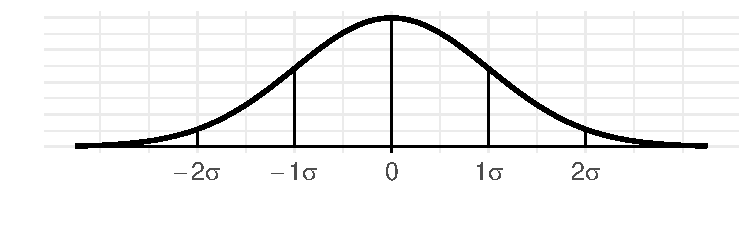
\includegraphics[width=\maxwidth]{img/mc-distribution-02-a-1} 

}







\begin{enumerate}
\item [\textbf{A} \msquare] Dargestellt ist eine Standardnormalverteilung.
\item [\textbf{B} \msquare] Die Fläche zwischen $-1\sigma$ und $1\sigma$ ist 0.95 und 95\% der Beobachtungen liegen somit zwischen $\bar{y}\pm\sigma$ in der obigen Verteilung.
\item [\textbf{C} \msquare] Die Fläche unter der Kurve entspricht dem Signifikanzniveau $\alpha$ von 5\%. Damit ist die Standardabweichung $\sigma$ gleich 1 in der obigen Abbildung.
\item [\textbf{D} \msquare] Es liegen 95\% der Beobachtungen zwischen $\bar{y}\pm 2 \sigma$. Angezeigt durch die Fläche zwischen $-2\sigma$ und $2\sigma$ in der obigen Verteilung.
\item [\textbf{E} \msquare] Die Fläche rechts von $2\sigma$ ist der p-Wert mit $Pr(D|H_0)$ in der obigen Abbildung.
\end{enumerate} 

\section{Aufgabe \hfill (2 Punkte)}

%% --------------------------------------------------------------------
\ifcollection
\begin{flushright}
\tiny\vspace{-2Ex}
\textbf{\examinhaltstart}
\exammodulestatversuch $\;\bullet$
\exammodulebiostat
\vspace{-1Ex}
\end{flushright}
\fi
%% --------------------------------------------------------------------




Mit einem Boxplot  können Sie sehr gut die Verteilung von Daten visualisieren. Die empfohlene Mindestanzahl an Beobachtungen ist dabei?



\begin{enumerate}
\item [\textbf{A} \msquare] Damit wir hier sauber eine Abbilung von einem 
\item [\textbf{B} \msquare] 1 Beobachtung.
\item [\textbf{C} \msquare] Wir sollten eine Beobachtung mindestens pro Gruppe vorliegen haben.
\item [\textbf{D} \msquare] Die untere Grenze liegt bei einer Beobachtung.
\item [\textbf{E} \msquare] Die untere Grenze liegt bei zwei bis fünf Beobachtungen.
\end{enumerate}

\section{Aufgabe \hfill (2 Punkte)}

%% --------------------------------------------------------------------
\ifcollection
\begin{flushright}
\tiny\vspace{-2Ex}
\textbf{\examinhaltstart}
\exammodulestatversuch $\;\bullet$
\exammodulebiostat
\vspace{-1Ex}
\end{flushright}
\fi
%% --------------------------------------------------------------------




Nach der Durchführung Ihres Feldexperiments wollen Sie eine ANOVA rechnen. Dafür muss aber Ihr Messwert zumindestens approximativ einer Normalverteilung folgen. Welche der drei Abbildungen erlaubt Ihnen abzuschätzen, ob Sie eine Normalverteilung in Ihrem Endpunkt vorliegen haben?





\begin{enumerate}
\item [\textbf{A} \msquare] Boxplot, Densityplot, Violinplot
\item [\textbf{B} \msquare] Histogramm, Scatterplot, Boxplot
\item [\textbf{C} \msquare] Violinplot, Scatterplot, Barplot
\item [\textbf{D} \msquare] Barplot, Mosaicplot, Violinplot
\item [\textbf{E} \msquare] Scatterplot, Mosaicplot, Boxplot
\end{enumerate}

\section{Aufgabe \hfill (2 Punkte)}


%% --------------------------------------------------------------------
\ifcollection
\begin{flushright}
\tiny\vspace{-2Ex}
\textbf{\examinhaltstart}
\exammodulestatversuch $\;\bullet$
\exammodulebiostat
\vspace{-1Ex}
\end{flushright}
\fi
%% --------------------------------------------------------------------




Sie wollen eine ANOVA im Anschluss an Ihr Feldexperiment rechnen. Dafür muss Ihr gemessener Endpunkt die Annahme einer Normalverteilung genügen. Zur Überprüfung können Sie folgende Visualisierung nutzen. Welche entsprechende Regel zur Abschätzung der Annahme einer Normalverteilung kommt zur Anwendung?



\begin{enumerate}
\item [\textbf{A} \msquare] Wir erstellen uns für jede Behandlung einen Boxplot und schauen, ob die Box und damit das IQR für jede Behandlung gleich groß ist.
\item [\textbf{B} \msquare] Einen Boxplot. Der Median, dargestellt als Linie, muss in der Mitte des IQR, dargestellt durch die Box, liegen.
\item [\textbf{C} \msquare] Einen Violinplot. Der Bauch der Violine muss hierbei einen höhren Wert annehmen als der Steg der Violine. Dann kann die Annahme einer Normalverteilung angenommen werden.
\item [\textbf{D} \msquare] Einen Dotplot. Die Punkte müssen sich wie an einer Perlenschnurr audreihen. Eine Abweichung führt zur Ablehnung der Annahme einer Normalverteilung.
\item [\textbf{E} \msquare] In einer explorativen Datanalyse nutzen wir den Violinplot. Dabei sollte der Bauch am Rand liegen. Dann können wir von einer Normalverteilung ausgehen.
\end{enumerate}
\section*{Statistische Testtheorie}  

\section{Aufgabe \hfill (2 Punkte)}

%% --------------------------------------------------------------------
\ifcollection
\begin{flushright}
\tiny\vspace{-2Ex}
\textbf{\examinhaltstart}
\exammodulemathstat $\;\bullet$
\exammodulestat $\;\bullet$
\exammodulestatbbv $\;\bullet$
\exammodulestatversuch $\;\bullet$
\exammodulebiostat
\vspace{-1Ex}
\end{flushright}
\fi
%% --------------------------------------------------------------------




Sie haben den mathematischen Ausdruck $Pr(D|H_0)$ vorliegen, welche Aussage ist richtig?



\begin{enumerate}
\item [\textbf{A} \msquare] $Pr(D|H_0)$ ist die Wahrscheinlichkeit der Alternativehypothese und somit $1 - Pr(H_A)$
\item [\textbf{B} \msquare] Die Wahrscheinlichkeit für die Nullhypothese, wenn die Daten wahr sind.
\item [\textbf{C} \msquare] Die Wahrscheinlichkeit der Daten unter der Nullhypothese in der Grundgesamtheit.
\item [\textbf{D} \msquare] $Pr(D|H_0)$ beschreibt die Wahrscheinlichkeit die Teststatistik $T_D$ aus den Daten $D$ zu beobachten, wenn die Nullhypothese wahr ist.
\item [\textbf{E} \msquare] $Pr(D|H_0)$ stellt die Wahrscheinlichkeit die Teststatistik $T$ zu beobachten dar, wenn die Nullhypothese falsch ist.
\end{enumerate} 

\section{Aufgabe \hfill (2 Punkte)}

%% --------------------------------------------------------------------
\ifcollection
\begin{flushright}
\tiny\vspace{-2Ex}
\textbf{\examinhaltstart}
\exammodulemathstat $\;\bullet$
\exammodulestat $\;\bullet$
\exammodulestatbbv $\;\bullet$
\exammodulestatversuch $\;\bullet$
\exammodulebiostat
\vspace{-1Ex}
\end{flushright}
\fi
%% --------------------------------------------------------------------




In fast allen wissenschaftlichen Disziplinen liegt der Grenzwert für das Signifikanzniveau $\alpha$ bei 5\%. Wieso wurde dieser Konsens über die Signifikanzschwelle in dieser Form getroffen?



\begin{enumerate}
\item [\textbf{A} \msquare] Der Wert ergab sich aus einer Auswertung von 1042 wissenschaftlichen Veröffentlichungen zwischen 1914 und 1948. Der Wert $5\%$ wurde in $28\%$ der Veröffentlichungen genutzt. Daher legte man sich auf diese Zahl fest.
\item [\textbf{B} \msquare] Da Wissenschaftler eine Schwelle für die statistische Testentscheidung benötigen wurde $\alpha$ historisch gewählt. Damit ist $\alpha = 5\%$ eine Kulturkonstante.
\item [\textbf{C} \msquare] Im Rahmen eines langen Disputs zwischen Neyman und Fischer wurde $\alpha = 5\%$ festgelegt. Leider werden die Randbedingungen und Voraussetzungen an statistsiche Modelle heute immer wieder ignoriert.
\item [\textbf{D} \msquare] Der Begründer der modernen Statistik, R. Fischer, hat die Grenze simuliert und berechnet. Dadurch ergibt sich dieser optimale Cut-Off.
\item [\textbf{E} \msquare] Da Wissenschaftler eine Schwelle für die statistische Testentscheidung benötigen wurde $\alpha$ in einer großen Konferenz 1945 gewählt. Damit ist $\alpha = 5\%$ eine Kulturkonstante mit einem Rank einer Naturkonstante.
\end{enumerate} 

\section{Aufgabe \hfill (2 Punkte)}

%% --------------------------------------------------------------------
\ifcollection
\begin{flushright}
\tiny\vspace{-2Ex}
\textbf{\examinhaltstart}
\exammodulemathstat $\;\bullet$
\exammodulestat $\;\bullet$
\exammodulestatbbv $\;\bullet$
\exammodulestatversuch $\;\bullet$
\exammodulebiostat
\vspace{-1Ex}
\end{flushright}
\fi
%% --------------------------------------------------------------------




Das statistische Testen basiert auf dem Falsifikationsprinzip. Es besagt,



\begin{enumerate}
\item [\textbf{A} \msquare] ... dass Fehlerterme in statistischen Modellen nicht verifiziert werden können.
\item [\textbf{B} \msquare] ... dass Annahmen an statistische Modelle meist falsch sind.
\item [\textbf{C} \msquare] ... dass ein schlechtes Modell durch ein schlechteres Modell ersetzt wird. Die Wissenschaft lehnt ab und verifiziert nicht.
\item [\textbf{D} \msquare] ... dass ein minderwertes Modell durch ein minderwertiges Modell ersetzt wird. Es gilt das Verifikationsprinzip nach Karl Popper.
\item [\textbf{E} \msquare] ... dass ein schlechtes Modell durch ein weniger schlechtes Modell ersetzt wird. Die Wissenschaft lehnt ab und verifiziert nicht.
\end{enumerate}

\section{Aufgabe \hfill (2 Punkte)}

%% --------------------------------------------------------------------
\ifcollection
\begin{flushright}
\tiny\vspace{-2Ex}
\textbf{\examinhaltstart}
\exammodulemathstat $\;\bullet$
\exammodulestat $\;\bullet$
\exammodulestatbbv $\;\bullet$
\exammodulestatversuch $\;\bullet$
\exammodulebiostat
\vspace{-1Ex}
\end{flushright}
\fi
%% --------------------------------------------------------------------




Betrachten wir die Teststatistik aus einem abstrakteren Blickwinkel. Beim statistischen Testen wird das 	extit{signal} mit dem 	extit{noise} aus den Daten $D$ zu einer Teststatistik $T_D$ verrechnet. Welche der Formel berechnet korrekt die Teststatistik $T_D$?



\begin{enumerate}
\item [\textbf{A} \msquare] Es gilt $T_D = \sfrac{noise}{signal}$. Der Effekt $noise$ wird mit der Varianz $signal$ gewichtet.
\item [\textbf{B} \msquare] Bei der Berechnung der Teststatistik $T_D$ gewichten wir den Effekt $signal$ mit der Varianz $noise$. Wir können verallgemeinert $T_D = \sfrac{signal}{noise}$ schreiben.
\item [\textbf{C} \msquare] Es gilt $T_D = signal \cdot noise$. Der Effekt $signal$ wird mit der Varianz $noise$ gewichtet.
\item [\textbf{D} \msquare] Es gilt $T_D = \sfrac{signal}{noise}$. Der Effekt $noise$ wird mit der Varianz $signal$ gewichtet.
\item [\textbf{E} \msquare] Bei der Berechnung der Teststatistik $T_D$ gewichten wir den Effekt $signal$ mit der Varianz $noise$. Wir können verallgemeinert $T_D = \sfrac{signal}{noise^2}$ schreiben.
\end{enumerate}

%% ------------------------------------------------------------

\section{Aufgabe \hfill (2 Punkte)}

%% --------------------------------------------------------------------
\ifcollection
\begin{flushright}
\tiny\vspace{-2Ex}
\textbf{\examinhaltstart}
\exammodulemathstat $\;\bullet$
\exammodulestat $\;\bullet$
\exammodulestatbbv $\;\bullet$
\exammodulestatversuch $\;\bullet$
\exammodulebiostat
\vspace{-1Ex}
\end{flushright}
\fi
%% --------------------------------------------------------------------




Sie haben ein Signifikanzniveau $\alpha$ gleich 5\% vorliegen. Welche Aussage zusammen mit dem $p$-Wert ist richtig?



\begin{enumerate}
\item [\textbf{A} \msquare] Wir machen ein Aussage über die Flächen unter der Kurve der Teststatistik der Hypothese $H_0$ und über die Flächen unter den Kurve der Teststatistik der Hypothese $H_A$. Dabei werden Wahrscheinlichkeiten vergleichen, die durch die Flächen unter der Kurve der beiden Testverteilungen repräsentiert werden.
\item [\textbf{B} \msquare] Wir vergleichen die Effekte des $p$-Wertes mit den Effekten der Signifikanzschwelle unter der Annahme der Nullhypothese. Dabei gilt, dass wir die Nullhypothese nur ablehnen können anhand des Falsifikationsprinzips.
\item [\textbf{C} \msquare] Wir vergleichen mit dem $p$-Wert und dem Signifikanzniveau $\alpha$ Wahrscheinlichkeiten und damit die Flächen unter der Kurve der Teststatistik, wenn die $H_0$ gilt.
\item [\textbf{D} \msquare] Wir vergleichen mit dem $p$-Wert und dem Signifikanzniveau $\alpha$ Wahrscheinlichkeiten und damit die absoluten Werte auf einem Zahlenstrahl, wenn die $H_0$ gilt.
\item [\textbf{E} \msquare] Wir vergleichen mit dem $p$-Wert und dem Signifikanzniveau $\alpha$ absolute Werte auf einem Zahlenstrahl und damit den Unterschied der Teststatistiken, wenn die $H_0$ gilt.
\end{enumerate}

\section{Aufgabe \hfill (2 Punkte)}

%% --------------------------------------------------------------------
\ifcollection
\begin{flushright}
\tiny\vspace{-2Ex}
\textbf{\examinhaltstart}
\exammodulemathstat $\;\bullet$
\exammodulestat $\;\bullet$
\exammodulestatbbv $\;\bullet$
\exammodulestatversuch $\;\bullet$
\exammodulebiostat
\vspace{-1Ex}
\end{flushright}
\fi
%% --------------------------------------------------------------------




Um die Testtheorie besser zu verstehen, mag es manchmal sinnvoll sein ein Beispiel aus dem Alltag zu wählen. Die Ergebnisse der Analyse durch einen statistischen Test können auch in grobe Analogie zur Wettervorhersage gebracht werden. Welche Aussage trifft am ehesten zu?



\begin{enumerate}
\item [\textbf{A} \msquare] In der Analogie der Regenwahrscheinlichkeit in einem bestimmten Gebiet: ein statistischer Test gibt die Wahrscheinlichkeit für ein Ereignis in einem Experiment mit den Daten $D$ wieder und lässt sich kaum verallgemeinern.
\item [\textbf{B} \msquare] In der Analogie der Maximaltemperatur: Was ist der maximale Unterschied zwischen zwei Gruppen. Wir erhalten hier eine Aussage über die Spannweite und den maximalen Effekt.
\item [\textbf{C} \msquare] In der Analogie der Regenwahrscheinlichkeit: ein statistischer Test gibt die Wahrscheinlichkeit für das Auftreten eines Ereignisses wieder. Die Stärke des Effektes wird nicht wiedergeben.
\item [\textbf{D} \msquare] In der Analogie der Durchschnittstemperatur: Wie oft tritt ein Effekt durchschnittlich ein? Wir erhalten eine Wahrscheinlichkeit für die Effekte. Zum Beispiel, wie hoch ist die Wahrscheinlichkeit für einen Mittelwert als Durchschnitt.
\item [\textbf{E} \msquare] In der Analogie der Sonnenscheindauer: Wie lange kann mit einem entsprechenden Effekt gerechnet werden? Die Wahrscheinlichkeit für den Effekt gibt der statistische Test wieder.
\end{enumerate}

\section{Aufgabe \hfill (2 Punkte)}

%% --------------------------------------------------------------------
\ifcollection
\begin{flushright}
\tiny\vspace{-2Ex}
\textbf{\examinhaltstart}
\exammodulemathstat $\;\bullet$
\exammodulestat $\;\bullet$
\exammodulestatbbv $\;\bullet$
\exammodulestatversuch $\;\bullet$
\exammodulebiostat
\vspace{-1Ex}
\end{flushright}
\fi
%% --------------------------------------------------------------------




In Ihrer Forschungsarbeit wollen Sie eine Aussage über ein untersuchtes Individuum treffen. Dazu nutzen Sie einen statistischen Test. Erhalten Sie eine valide Aussage aus einem statistischen Test?



\begin{enumerate}
\item [\textbf{A} \msquare] Nein, wir können ein untersuchtes Individuum nicht mit einem t-Test auswerten. Wir erhalten keine Aussage zum Individuum. Wir können aber den Effekt als Quelle der Relevanz nutzen.
\item [\textbf{B} \msquare] Weder eine Ausssage über die Population noch über das Individuum ist mit einem statistischen Test möglich. Wir erhalten eine Aussage über ein Experiment.
\item [\textbf{C} \msquare] Nein, ein untersuchtes Individuum können wir mit einem statistischen Test nicht auswerten. Wir erhalten keine Aussage zum Individuum.
\item [\textbf{D} \msquare] Nein, wir können ein untersuchtes Individuum nicht mit einer ANOVA auswerten. Wir erhalten keine Aussage zum Individuum. Wir können aber den Test adjustieren und so die Auswertung ermöglichen.
\item [\textbf{E} \msquare] Ja, ein untersuchtes Individuum können wir mit einem statistischen Test auswerten. Wir erhalten dann eine Aussage zum Individuum.
\end{enumerate}

\section{Aufgabe \hfill (2 Punkte)}

%% --------------------------------------------------------------------
\ifcollection
\begin{flushright}
\tiny\vspace{-2Ex}
\textbf{\examinhaltstart}
\exammodulemathstat $\;\bullet$
\exammodulestat $\;\bullet$
\exammodulestatbbv $\;\bullet$
\exammodulestatversuch $\;\bullet$
\exammodulebiostat
\vspace{-1Ex}
\end{flushright}
\fi
%% --------------------------------------------------------------------




Sie rechnen einen statistischen Test und erhalten neben dem p-Wert noch einen Effekt wiedergegeben. Welche Aussage zum Effekt ist richtig?



\begin{enumerate}
\item [\textbf{A} \msquare] Der Effekt eines statistischen Tests beschreibt die biologisch interpretierbare Ausgabe eines Tests. Zum Beispiel den mittleren Unterschied zwischen zwei Gruppen aus einem t-Test. Damit ist der Effekt direkt mit dem Begriff der Relevanz verbunden. Die Entscheidung über die Relevanz trifft der Forschende unabhängig von der Signifikanz eines statistischen Tests.
\item [\textbf{B} \msquare] Der Effekt eines statistischen Tests beschreibt die biologisch interpretierbare Ausgabe eines Tests. Moderen Algorithmen liefern keine Effekte mehr sondern nur noch bedingte Wahrscheinlichkeiten. Der Effekt spielt in der modernen Statistik keine Rollen mehr.
\item [\textbf{C} \msquare] Der Effekt eines statistischen Tests beschreibt die biologisch interpretierbare Ausgabe eines Tests. Damit ist der Effekt direkt mit dem Begriff der Signifikanz verbunden. Die Entscheidung über die Signifikanz trifft der Forschende unabhängig von der Relevanz eines statistsichen Tests.
\item [\textbf{D} \msquare] Der Effekt eines statistischen Tests beschreibt den Output oder die Wiedergabe eines Tests in einem Computer.
\item [\textbf{E} \msquare] Der Effekt eines statistischen Tests beschreibt die mathematisch interpretierbare Ausgabe eines Tests. Damit ist der Effekt direkt mit dem Begriff der Signifikanz verbunden. Die Entscheidung über die Signifikanz trifft der Forschende unabhängig von der Relevanz eines statistsichen Tests.
\end{enumerate}

\section{Aufgabe \hfill (2 Punkte)}

%% --------------------------------------------------------------------
\ifcollection
\begin{flushright}
\tiny\vspace{-2Ex}
\textbf{\examinhaltstart}
\exammodulemathstat $\;\bullet$
\exammodulestat $\;\bullet$
\exammodulestatbbv $\;\bullet$
\exammodulestatversuch $\;\bullet$
\exammodulebiostat
\vspace{-1Ex}
\end{flushright}
\fi
%% --------------------------------------------------------------------



Roland Fischer entwickelte Anfang des letzten Jahrhunderts als Grundlage für das experimentelle Design in der Statistik die Randomisierung. Warum ist die Randomisierung für die Entscheidung anhand einer statistischen Auswertung so wichtig?



\begin{enumerate}
\item [\textbf{A} \msquare] Randomisierung ist die direkte Folge von Strukturgleichheit. Die Strukturgleichheit erlaubt es erst von der Stichprobe auf die Grundgesamtheit zurückzuschliessen.
\item [\textbf{B} \msquare] Strukturgleichheit ist durch Randomisierung gegeben. Leider hilft die Randomisierung noch nicht um von der Stichprobe auf die Grundgesamtheit zu schließen. Deshalb wurde das Falsifikationsprinzip entwickelt.
\item [\textbf{C} \msquare] Randomisierung erlaubt erst die Varianzen zu schätzen. Ohne eine Randomisierung ist die Berechnung von Mittelwerten und Varianzen nicht möglich. Dadurch lässt sich erst ein Experiment auswerten.
\item [\textbf{D} \msquare] Strukturgleichheit ist durch Randomisierung gegeben. Somit kann von der Stichprobe auf die Grundgesamtheit geschlossen werden
\item [\textbf{E} \msquare] Randomisierung war bis 1952 bedeutend, wurde dann aber in Folge besserer Rechnerleistung nicht mehr verwendet. Aktuelle Statistik nutzt keine Randomisierung mehr.
\end{enumerate}

\section{Aufgabe \hfill (2 Punkte)}

%% --------------------------------------------------------------------
\ifcollection
\begin{flushright}
\tiny\vspace{-2Ex}
\textbf{\examinhaltstart}
\exammodulemathstat $\;\bullet$
\exammodulestat $\;\bullet$
\exammodulestatbbv $\;\bullet$
\exammodulestatversuch $\;\bullet$
\exammodulebiostat
\vspace{-1Ex}
\end{flushright}
\fi
%% --------------------------------------------------------------------




Ein statistischer Test benötigt für die richtige Durchführung Hypothesen $H$, sonst ist der Test nicht zu interpretieren. Welche Aussage ist richtig?



\begin{enumerate}
\item [\textbf{A} \msquare] Mit der Nullhypothese $H_A$ und der Alternativehypothese $H_0$ gibt es zwei Hypothesen, die aber selten genutzt werden.
\item [\textbf{B} \msquare] Ein statistisches Hypothesenpaare gibt es. Zum einen die Nullhypothese und zum anderen die Alternativehypothese. Es ist aber nur notwendig die Alternative anzugeben, da die Nullhypothese nicht beim Testen benötigt wird.
\item [\textbf{C} \msquare] Es gibt ein statistisches Hypothesenpaar mit der Hypothese für und gegen die wissenschaftliche Fragestellung. Die Hypothesen werden $H_{pro}$ und $H_{contra}$ bezeichnet.
\item [\textbf{D} \msquare] Die Hypothesen $H_0$ und $H_A$ sind rein prosarischer Natur und bilden keinen mathematischen Hintergrund ab. In der Statistik wird die wissenschaftliche Fragestellung getestet. Daher stehen auch die verständlichen Hypothesen im Mittelpunkt der biologischen Interpretation.
\item [\textbf{E} \msquare] Mit der Nullhypothese $H_0$ und der Alternativehypothese $H_A$ oder $H_1$ gibt es zwei Hypothesen.
\end{enumerate}

\section{Aufgabe \hfill (2 Punkte)}

%% --------------------------------------------------------------------
\ifcollection
\begin{flushright}
\tiny\vspace{-2Ex}
\textbf{\examinhaltstart}
\exammodulemathstat $\;\bullet$
\exammodulestat $\;\bullet$
\exammodulestatbbv $\;\bullet$
\exammodulestatversuch $\;\bullet$
\exammodulebiostat
\vspace{-1Ex}
\end{flushright}
\fi
%% --------------------------------------------------------------------




Sie versuchen folgende Aussage richtig in die Analogie der statistischen Testtheorie zu setzen. Welche Analogie ist richtig?

\begin{center}
\textit{$H_0$ beibehalten obwohl die $H_0$ falsch ist}
\end{center}



\begin{enumerate}
\item [\textbf{A} \msquare] \textit{Fire without alarm}, dem $\beta$-Fehler als Analogie eines Rauchmelders.
\item [\textbf{B} \msquare] \textit{Fire without alarm}, dem $\beta$-Fehler als Analogie von Rauch im Haus.
\item [\textbf{C} \msquare] \textit{Alarm with fire}, dem $\alpha$-Fehler in der Analogie von Feuer.
\item [\textbf{D} \msquare] In die Analogie eines Rauchmelders: \textit{Alarm without fire police}, dem $\alpha$-Fehler.
\item [\textbf{E} \msquare] In die Analogie eines Rauchmelders: \textit{Alarm without fire}, dem $\alpha$-Fehler.
\end{enumerate}

\section{Aufgabe \hfill (2 Punkte)}

%% --------------------------------------------------------------------
\ifcollection
\begin{flushright}
\tiny\vspace{-2Ex}
\textbf{\examinhaltstart}
\exammodulestat $\;\bullet$
\exammodulestatbbv $\;\bullet$
\exammodulestatversuch $\;\bullet$
\exammodulebiostat
\vspace{-1Ex}
\end{flushright}
\fi
%% --------------------------------------------------------------------




Sie lesen eine wissenschaftliche Arbeit, die damit wirbt, dass Effekte und Signifikanz nicht separat dargestellt sind, sondern in einer statistischen Maßzahl zusammen. Welche Aussage ist richtig?



\begin{enumerate}
\item [\textbf{A} \msquare] Die Teststatistik. Durch den Vergleich von $T_c$ zu $T_k$ ist es m{"o}glich die $H_0$ abzulehnen. Die Relevanz ergibt sich aus der Fläche rechts vom dem $T_c$-Wert.
\item [\textbf{B} \msquare] Das OR. Als Chancenverhältnis gibt es das Verhältnis von Relevanz und Signifikanz wieder.
\item [\textbf{C} \msquare] Der p-Wert. Durch den Vergleich mit $\alpha$ lässt sich über die Signifikanz entscheiden und der $\beta$-Fehler erlaubt über die Power eine Einschätzung der Relevanz.
\item [\textbf{D} \msquare] Einem Konfidenzintervall. Das Konfidenzinterval bringt durch eine Visualisierung und zwei Intervallgrenzen die Möglichkeit mit, eine Relevanzschwelle neben der definierten Signifikanzschwelle zu definieren.
\item [\textbf{E} \msquare] Das $\Delta$. Durch die Effektstärke haben wir einen Wert für die Relevanz, die vom Anwender bewertet werden muss. Da $\Delta$ antiproportional zum p-Wert ist, bedeutet auch ein hohes $\Delta$ ein sehr kleinen p-Wert.
\end{enumerate}

\section{Aufgabe \hfill (2 Punkte)}

%% --------------------------------------------------------------------
\ifcollection
\begin{flushright}
\tiny\vspace{-2Ex}
\textbf{\examinhaltstart}
\exammodulestatversuch $\;\bullet$
\exammodulebiostat
\vspace{-1Ex}
\end{flushright}
\fi
%% --------------------------------------------------------------------




In der Bio Data Science wird häufig mit sehr großen Datensätzen gerechnet. Historisch ergibt sich nun ein Problem bei der Auswertung der Daten und deren Bewertung hinsichtlich der Signifikanz. Welche Aussage ist richtig?





\begin{enumerate}
\item [\textbf{A} \msquare] Aktuell werden immer größere Datensätze erhoben. Dadurch wird auch die Varianz immer höher was automatisch zu mehr signifikanten Ergebnissen führt.
\item [\textbf{B} \msquare] Mehr Fallzahl in Datensätzen bedeutet mehr signifikante Ergebnisse, da in mehr Daten auch mehr Informationen beinhaltet sind. Deshalb lohnen sich riesige Datensätze, die durch die vielen signifikanten Ergebnisse auch eine Menge an relevanten Erkenntnissen liefern.
\item [\textbf{C} \msquare] Eine erhöhte Fallzahl führt automatisch zu mehr signifikanten Ergebnissen auch wenn der Effekt klein ist und damit nicht relevant. Dadurch sind die Informationen zur Signifikanz in riesigen Datensätzen schwer zu verwerten, da fast alle Vergleiche signifikant sind.
\item [\textbf{D} \msquare] Big Data ist ein Problem der parametrischen Statistik. Parameter lassen sich nur auf kleinen Datensätzen berechnen, da es sich sonst nicht mehr um eine Stichprobe im engen Sinne der Statistik handelt.
\item [\textbf{E} \msquare] Riesige Datensätz haben mehr Fallzahl was zur $\alpha$-Inflation führt. Durch eine Adjustoerung kann dem Problem entgegengewirkt werden.
\end{enumerate}

\section{Aufgabe \hfill (2 Punkte)}

%% --------------------------------------------------------------------
\ifcollection
\begin{flushright}
\tiny\vspace{-2Ex}
\textbf{\examinhaltstart}
\exammodulestatversuch $\;\bullet$
\exammodulebiostat
\vspace{-1Ex}
\end{flushright}
\fi
%% --------------------------------------------------------------------




Im Rahmen Ihrer Abschlussarbeit werten Sie ein Experiment mit Ferkel aus. Es geht um die Leistungssteigerung der Ferkelproduktion. Sie messen jeweils die Gewichtszunahme der Ferkel. Die Ferkel einer Muttersau sind dabei...



\begin{enumerate}
\item [\textbf{A} \msquare] Untereinander abhängig, wenn die Mütter ebenfalls miteinander verwandt sind. Erst die Abhängigkeit 2. Grades wird in der Statistik modelliert.
\item [\textbf{B} \msquare] Je nach Stallanlage kommt eine andere Analyse in Betracht. Eine allgemeine Aussage über Ferkel und Sauen lässt sich statistisch nicht treffen.
\item [\textbf{C} \msquare] Untereinander abhängig. Die Ferkel stammen von einem Muttertier und haben vermutliche eine ähnliche Varianzstruktur.
\item [\textbf{D} \msquare] Die Ferkel stammen von der gleichen Sau und sind somit untereinander unabhängig.
\item [\textbf{E} \msquare] Untereinander unabhängig. Sollten die Mütter verwandt sein, so ist die Varianzstruktur ähnlich und muss modelliert werden.
\end{enumerate}

\section{Aufgabe \hfill (2 Punkte)}

%% --------------------------------------------------------------------
\ifcollection
\begin{flushright}
\tiny\vspace{-2Ex}
\textbf{\examinhaltstart}
\exammodulestatversuch $\;\bullet$
\exammodulebiostat
\vspace{-1Ex}
\end{flushright}
\fi
%% --------------------------------------------------------------------






Nachdem Sie einen t-Test gerechnet haben stehen Ihnen verschiedene statistische Maßzahlen zu Verfügung um eine Entscheidung gegen die Nullhypothese zu treffen. Sie entscheiden sich anhand des 95\%-Konfidenzintervalls eine Entscheidung zu treffen.





\begin{enumerate}
\item [\textbf{A} \msquare] Liegt das berechnete Intervall über dem kritische Wert $T_{\alpha = 5\%}$, dann kann die Nullhypothese nicht abgelehnt werden.
\item [\textbf{B} \msquare] Ist $Pr(D|H_0)$ kleiner als das Signifikanzniveau $\alpha$ gleich $5\%$ dann wird die Nullhypothese $H_0$ abgelehnt.
\item [\textbf{C} \msquare] Das Signifikanzniveauintervall $\alpha$ ist gleich $5\%$ und damit muss das berechnete Intervall unter dem Signifikanzniveauintervall $\alpha$ liegen, dann kann die Nullhypothese nicht abgelehnt werden.
\item [\textbf{D} \msquare] Wir betrachten das Ganze Intervall des 95\%-Konfidenzintervalls. Liegt die Null mit in dem Intervall, dann kann die Nullhypothese abgelehnt werden.
\item [\textbf{E} \msquare] Ist $T_{D}$ höher als der kritische Wert $T_{\alpha = 5\%}$ dann wird die Nullhypothese $H_0$ abgelehnt.
\end{enumerate}

\section{Aufgabe \hfill (2 Punkte)}

%% --------------------------------------------------------------------
\ifcollection
\begin{flushright}
\tiny\vspace{-2Ex}
\textbf{\examinhaltstart}
\exammodulebiostat
\vspace{-1Ex}
\end{flushright}
\fi
%% --------------------------------------------------------------------




Welche Aussage über die \textit{Power} ist richtig?



\begin{enumerate}
\item [\textbf{A} \msquare] Die Power ist nicht in der aktuellen Testthorie mehr vertreten. Wir rechnen nur noch mit dem Fehler 1. Art.
\item [\textbf{B} \msquare] Die Power beschreibt die Wahrscheinlichkeit die $H_A$ abzulehnen. Wir testen die Power jedoch nicht.
\item [\textbf{C} \msquare] Die Power wird berechnet und ist keine Eigenschaft des Tests. Die Power wird auf $80\%$ gesetzt und beschreibt mit welcher Wahrscheinlichkeit $H_0$ \textit{bewiesen wird}
\item [\textbf{D} \msquare] Die Power $1-\beta$ wird auf 80\% gesetzt. Damit liegt die Wahrscheinlichkeit für die $H_0$ bei 20\%.
\item [\textbf{E} \msquare] Die Power $1-\beta$ wird auf 80\% gesetzt. Alle statistischen Tests sind so konstruiert, dass die $H_A$ mit 80\% \textit{bewiesen wird}.
\end{enumerate}
\section*{Statistische Tests für Gruppenvergleiche} 

\section{Aufgabe \hfill (2 Punkte)}

%% --------------------------------------------------------------------
\ifcollection
\begin{flushright}
\tiny\vspace{-2Ex}
\textbf{\examinhaltstart}
\exammodulemathstat $\;\bullet$
\exammodulestat $\;\bullet$
\exammodulestatbbv 
\vspace{-1Ex}
\end{flushright}
\fi
%% --------------------------------------------------------------------




Welche Aussage über den t-Test im Allgmeinen ist richtig? Berücksichtigen Sie den Welch t-Test wie auch den Student t-Test!



\begin{enumerate}
\item [\textbf{A} \msquare] Der t-Test vergleicht zwei oder mehr Gruppen indem die Mittelwerte miteinander verglichen werden.
\item [\textbf{B} \msquare] Der t-Test ist ein Vortest der ANOVA und basiert daher auf dem Vergleich von Streuungsparametern
\item [\textbf{C} \msquare] Der t-Test vergleicht die Mittelwerte von zwei Gruppen.
\item [\textbf{D} \msquare] Der t-Test testet generell zu einem erhöhten $\alpha$-Niveau von 20\%.
\item [\textbf{E} \msquare] Der t-Test vergleicht die Mittelwerte von zwei Gruppen unter der strikten Annahme von Varianzhomogenität. Sollte keine Varianzhomogenität vorliegen, so gibt es keine Möglichkeit den t-Test in einer Variante anzuwenden.
\end{enumerate}

\section{Aufgabe \hfill (2 Punkte)}

%% --------------------------------------------------------------------
\ifcollection
\begin{flushright}
\tiny\vspace{-2Ex}
\textbf{\examinhaltstart}
\exammodulestatversuch $\;\bullet$
\exammodulebiostat
\vspace{-1Ex}
\end{flushright}
\fi
%% --------------------------------------------------------------------





Sie rechnen einen gepaarten t-Test, da Ihre Beobachtungen verbunden sind. Welche der folgenden Aussagen ist richtig?



\begin{enumerate}
\item [\textbf{A} \msquare] Wenn die Beobachtungen unabhängig voneinander sind, rechnen wir einen gepaarten t-Test. Messen wir wiederholt an dem gleichen Tier oder Pflanze dann bilden wir das Produkt zwischen den zwei Messpunkten.
\item [\textbf{B} \msquare] Abhängige Beobachtungen müssen gesondert in einem gepaarten t-Test modelliert werden. Wenn wiederholt an dem gleichen Tier oder Pflanze gemessen wird, dann bilden wir die Differenz zwischen den beiden Zeitpunkten. Auf den Differenzen rechnen wir den gepaarten t-Test.
\item [\textbf{C} \msquare] Der gepaarte t-Test nutzt die Varianz der Beobachtungen jeweils paarweise und bildet dafür eine verbundene Stichprobe. Dieser Datensatz $d$ dient dann zur Differenzbildung.
\item [\textbf{D} \msquare] Der gepaarte t-Test wird gerechnet, wenn die Beobachtungen abhängig voneinander sind. Wir messen jede Beobachtung nur einmal und berechnen dann die Differenz zu dem Mittel der anderen Beobachtungen.
\item [\textbf{E} \msquare] Abhängige Beobachtungen müssen gesondert in einem gepaarten t-Test modelliert werden. Wenn wiederholt an dem gleichen Tier oder Pflanze gemessen wird, dann bilden wir den Quotienten zwischen den beiden Zeitpunkten. Auf den Quotienten rechnen wir den gepaarten t-Test.
\end{enumerate}

\section{Aufgabe \hfill (2 Punkte)}

%% --------------------------------------------------------------------
\ifcollection
\begin{flushright}
\tiny\vspace{-2Ex}
\textbf{\examinhaltstart}
\exammodulemathstat $\;\bullet$
\exammodulestat $\;\bullet$
\exammodulestat $\;\bullet$
\exammodulestatbbv $\;\bullet$
\exammodulestatversuch $\;\bullet$
\exammodulebiostat
\vspace{-1Ex}
\end{flushright}
\fi
%% --------------------------------------------------------------------




Die folgende Abbildung enthält die Daten aus einer Studie zur Bewertung der Wirkung des Mikronährstoff Sulfit auf den Ertrag in t/ha von Weizen im Vergleich zu einer Kontrolle. Der Versuch wurde in 13 Parzellen pro Gruppe durchgeführt. Welche Aussage im Bezug auf eine statistische Auswertung ist richtig?



{\centering 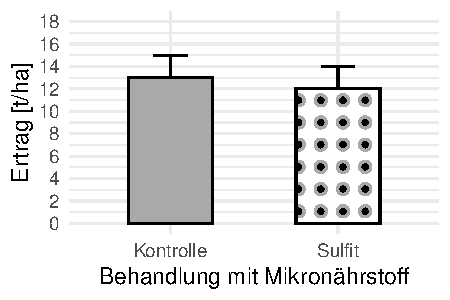
\includegraphics[width=\maxwidth]{img/mc-testing-ttest-02-1} 

}







\begin{enumerate}
\item [\textbf{A} \msquare] Es liegt ein signifikanter Unterschied vor. Der Effekt liegt bei -0.1.
\item [\textbf{B} \msquare] Die Barplots deuten auf ein signifikanten Unterschied. Der Effekt liegt vermutlich bei -1.
\item [\textbf{C} \msquare] Die Barplots deuten auf keinen signifikanten Unterschied. Der Effekt liegt vermutlich bei -1 unter einer groben Abschätzung. Wir müssen aber eine ANOVA rechnen um den Effekt wirklich bestimmen zu können.
\item [\textbf{D} \msquare] Nach Betrachtung des Barplots liegt kein signifikanter Unterschied vor. Der Effekt kann nicht bei einem t-Test aus Barplots bestimmt werden.
\item [\textbf{E} \msquare] Die Barplots deuten auf keinen signifikanten Unterschied. Der Effekt liegt vermutlich bei -1 unter einer groben Abschätzung.
\end{enumerate}

\section{Aufgabe \hfill (2 Punkte)}

%% --------------------------------------------------------------------
\ifcollection
\begin{flushright}
\tiny\vspace{-2Ex}
\textbf{\examinhaltstart}
\exammodulestatversuch $\;\bullet$
\exammodulebiostat
\vspace{-1Ex}
\end{flushright}
\fi
%% --------------------------------------------------------------------




Sie führen paarweise t-Tests für alle Vergleiche der verschiedenen Rapssorten in Ihrem Experiment durch. Nach der Adjustierung für multiples Testen ist kein p-Wert unter der $\alpha$-Schwelle. Ihr Experiment beinhaltet fünf Rapssorten und eine ANOVA ergibt $p = 0.049$ für den Ertrag. Sie schauen sich auch die rohen, unadjustierten p-Werte an und finden hier als niedrigsten p-Wert $p_{3-2} = 0.053$. Welche Aussage ist richtig?




\begin{enumerate}
\item [\textbf{A} \msquare] Das Beispiel kann so nicht auftreten, da die ANOVA und die t-Tests algorithmisch miteinander verschränkt sind.
\item [\textbf{B} \msquare] Die adjustierten p-Werte deuten in die richtige Richtung. Zusammen mit den nicht signifikanten rohen p-Werten ist von einem Fehler in der ANOVA auszugehen.
\item [\textbf{C} \msquare] Der Fehler liegt in den t-Tests. Wenn eine ANOVA signifikant ist, dann muss zwangsweise auch ein t-Test signifikant sein.
\item [\textbf{D} \msquare] Hier kommt der Effekt der stiegenden Fallzahl auf die Anzahl an signifikante Ergebnisse zu tragen. Da die ANOVA auf weniger Fallzahl testet als die paarweisen t-Tests, kann die ANOVA schwerer einen signifikanten Unterscheid nachweisen.
\item [\textbf{E} \msquare] Das ist kein Wunder. Die ANOVA testet auf der gesamten Fallzahl und die paarweisen t-Tests verlieren immer eine oder mehr Gruppen als Fallzahl. Mit steigender Fallzahl sind mehr signifikante Unterschiede zu erwarten. Die p-Werte unterscheiden sich numerisch auch kaum.
\end{enumerate}
\section*{ANOVA}

\section{Aufgabe \hfill (2 Punkte)}

%% --------------------------------------------------------------------
\ifcollection
\begin{flushright}
\tiny\vspace{-2Ex}
\textbf{\examinhaltstart}
\exammodulemathstat $\;\bullet$
\exammodulestat $\;\bullet$
\exammodulestatbbv $\;\bullet$
\exammodulestatversuch $\;\bullet$
\exammodulebiostat
\vspace{-1Ex}
\end{flushright}
\fi
%% --------------------------------------------------------------------






Aus einem Feldversuch ergibt sich die Notwendigkeit der Berechnung einer einfaktoriellen ANOVA. Es ergibt sich ein $\eta^2 = 0.78$. Welche Aussage ist richtig?



\begin{enumerate}
\item [\textbf{A} \msquare] Der Anteil der Varianz, der von den Behandlungsbedingungen erklärt wird, wird durch das $\eta^2$ beschrieben.
\item [\textbf{B} \msquare] Die Berechnung von $\eta^2$ ist ein Wert für die Interaktion in der einfaktoriellen ANOVA.
\item [\textbf{C} \msquare] Das $\eta^2$ ist die Korrelation der ANOVA. Mit der Ausnahme, dass $\eta^2 = 0$ der beste Wert ist.
\item [\textbf{D} \msquare] Das $\eta^2$ beschreibt den Anteil der Varianz, der von den Behandlungsbedingungen nicht erklärt wird. Somit der Rest an nicht erklärbarer Varianz.
\item [\textbf{E} \msquare] Der Anteil der Varianz, der von den Behandlungsbedingungen erklärt wird, wird durch das $1-\eta^2$ beschrieben.
\end{enumerate}

\section{Aufgabe \hfill (2 Punkte)}

%% --------------------------------------------------------------------
\ifcollection
\begin{flushright}
\tiny\vspace{-2Ex}
\textbf{\examinhaltstart}
\exammodulemathstat $\;\bullet$
\exammodulestat $\;\bullet$
\exammodulestatbbv $\;\bullet$
\exammodulestatversuch $\;\bullet$
\exammodulebiostat
\vspace{-1Ex}
\end{flushright}
\fi
%% --------------------------------------------------------------------










\begin{enumerate}
\item [\textbf{A} \msquare] Es werden 20\% der Varianz durch den Versuch erklärt. Das $\eta^2$ beschreibt den Anteil der Varianz, der durch Fehler in der Versuchsdurchführung entsteht.
\item [\textbf{B} \msquare] Mit dem $\eta^2$ lässt sich auf die Qualität der Randomisierung und damit der Strukturgleichheit zwischen der Grundgesamtheit und der Stichprobe schließen. Es gilt dabei die Regel, dass ein $\eta^2$-Wert von 1 zu bevorzugen ist.
\item [\textbf{C} \msquare] Es werden 80\% der Varianz durch die Behandlung erklärt. Das $\eta^2$ beschreibt den Anteil der Varianz, der von den unterschiedlichen Behandlungsbedingungen nicht erklärt wird.
\item [\textbf{D} \msquare] Das $\eta^2$ beschreibt den Anteil der Varianz, der von den Behandlungsbedingungen erklärt wird. Daher werden 20\% der Varianz erklärt.
\item [\textbf{E} \msquare] Das $\eta^2$ beschreibt den Anteil der Varianz, der durch den Forschenden entsteht. Es gilt die Regel, dass ca. 70\% der Varianz eines Versuches durch die Versuchsdurchführung entstehen sollen.
\end{enumerate}

\section{Aufgabe \hfill (2 Punkte)}

%% --------------------------------------------------------------------
\ifcollection
\begin{flushright}
\tiny\vspace{-2Ex}
\textbf{\examinhaltstart}
\exammodulemathstat $\;\bullet$
\exammodulestat $\;\bullet$
\exammodulestatbbv $\;\bullet$
\exammodulestatversuch $\;\bullet$
\exammodulebiostat
\vspace{-1Ex}
\end{flushright}
\fi
%% --------------------------------------------------------------------




Eine einfaktorielle ANOVA berechnet eine Teststatistik um zu die Nullhypothese abzulehnen. Welche Aussage über die Teststatistik der ANOVA ist richtig?



\begin{enumerate}
\item [\textbf{A} \msquare] Die ANOVA berechnet die F-Statistik indem die MS des Fehlers durch die MS der Behandlung geteilt werden. Wenn die F-Statistik sich der 0 ann{"a}hert kann die Nullhypothese abgelehnt werden.
\item [\textbf{B} \msquare] Die ANOVA berechnet die T-Statistik aus der Multiplikation der MS Behandlung mit der MS der Fehler. Wenn die F-Statistik genau 0 ist, kann die Nullhypothese nicht abgelehnt werden.
\item [\textbf{C} \msquare] Die ANOVA berechnet die T-Statistik indem den Mittelwertsunterschied der Gruppen simultan durch die Standardabweichung der Gruppen teilt. Wenn die T-Statistik h{"o}her als 1.96 ist, kann die Nullhypothese abgelehnt werden.
\item [\textbf{D} \msquare] Die ANOVA berechnet die F-Statistik indem die MS der Behandlung durch die MS des Fehlers geteilt werden. Wenn die F-Statistik sich der 0 ann{"a}hert kann die Nullhypothese nicht abgelehnt werden.
\item [\textbf{E} \msquare] Die ANOVA berechnt die F-Statistik aus den SS Behandlung geteilt durch die SS Fehler.
\end{enumerate}

\section{Aufgabe \hfill (2 Punkte)}

%% --------------------------------------------------------------------
\ifcollection
\begin{flushright}
\tiny\vspace{-2Ex}
\textbf{\examinhaltstart}
\exammodulemathstat $\;\bullet$
\exammodulestat $\;\bullet$
\exammodulestatbbv $\;\bullet$
\exammodulestatversuch $\;\bullet$
\exammodulebiostat
\vspace{-1Ex}
\end{flushright}
\fi
%% --------------------------------------------------------------------




Viele statistische Verfahren nutzen eine Teststatistik um eine Aussage über den Zusammenhang zwischen der Grundgesamthat und der Stichprobe abzubilden. Ein statistisches Testwerkzeug ist hierbei die ANOVA. Die ANOVA rechnet dabei...



\begin{enumerate}
\item [\textbf{A} \msquare] ... den Unterschied zwischen der Varianz ausgelöst durch alle Behandlungsgruppen und der Varianz aus globalen Behandlungsguppen der Kontrollen. Wenn die ANOVA nicht signifikant ist, muss ein Posthoc-Test ausgeschlossen werden.
\item [\textbf{B} \msquare] ... den Unterschied zwischen der Varianz aus verschiedenen Behandlungsguppen und der Varianz über alle Behandlungsgruppen. Wenn die ANOVA signifikant ist, muss über einen Posthoc-Test nachgedacht werden um den signifikanten Unterschied in den Gruppen exakt zu bestimmen.
\item [\textbf{C} \msquare] ... den Unterschied zwischen der Mittelwerte und der Varianz aus verschiedenen Behandlungsguppen. Wenn die ANOVA signifikant ist, ist bekannt welcher Vergleich konkret unterschiedlich ist.
\item [\textbf{D} \msquare] ... den Unterschied zwischen der F-Statistik anhand der Varianz der Gruppen. Wenn die F-Statistik exakt 0 ist, kann die Nullhypothese abgelehnt werden.
\item [\textbf{E} \msquare] ... den Unterschied zwischen zwei paarweisen Mittelwerten aus verschiedenen Behandlungsguppen. Wenn die signifikant ist, ist daher bekannt welcher Vergleich konkret unterschiedlich ist.
\end{enumerate}

\section{Aufgabe \hfill (2 Punkte)}

%% --------------------------------------------------------------------
\ifcollection
\begin{flushright}
\tiny\vspace{-2Ex}
\textbf{\examinhaltstart}
\exammodulestatversuch $\;\bullet$
\exammodulebiostat
\vspace{-1Ex}
\end{flushright}
\fi
%% --------------------------------------------------------------------




Ein Versuch wurde an 65 Tieren durchgeführt, wobei jedes Tier eine von drei Vitamin-C-Dosen (0.5, 1 und 1.5 mg/Tag) über eine von zwei Verabreichungsmethoden erhielt. Die folgende Abbildung enthält die Daten aus diesem Versuch zur Bewertung der Wirkung von Vitamin C auf das Zahnwachstum bei Hasen.  Welche Aussage ist richtig, wenn Sie eine zweifaktorielle ANOVA rechnen?



{\centering 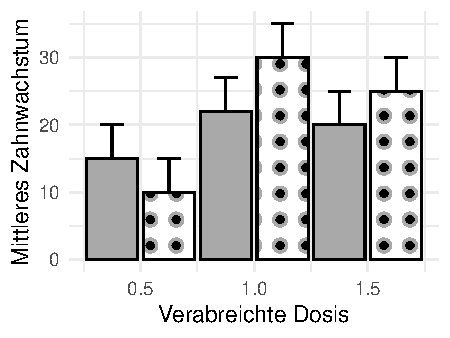
\includegraphics[width=\maxwidth]{img/mc-anova-02-a-1} 

}







\begin{enumerate}
\item [\textbf{A} \msquare] Keine Interaktion liegt vor $(p \leq 0.05)$.
\item [\textbf{B} \msquare] Eine mittlere bis starke Interaktion liegt vor $(p \leq 0.05)$
\item [\textbf{C} \msquare] Keine Korrelation liegt vor $(p \geq 0.05)$.
\item [\textbf{D} \msquare] Eine negative Interaktion liegt vor $(\rho \geq 0.5)$.
\item [\textbf{E} \msquare] Eine positive Interaktion liegt vor $(\rho \leq -0.5)$ 
\end{enumerate}
\section*{Multiple Gruppenvergleiche} 

\section{Aufgabe \hfill (2 Punkte)}

%% --------------------------------------------------------------------
\ifcollection
\begin{flushright}
\tiny\vspace{-2Ex}
\textbf{\examinhaltstart}
\exammodulestatversuch $\;\bullet$
\exammodulebiostat
\vspace{-1Ex}
\end{flushright}
\fi
%% --------------------------------------------------------------------




Sie haben folgende unadjustierten p-Werte gegeben: 0.34, 0.89, 0.21 und 0.03. Sie adjustieren die p-Werte nach
Bonferroni. Welche Aussage ist richtig?



\begin{enumerate}
\item [\textbf{A} \msquare] Nach der Bonferroni-Adjustierung ergeben sich die adjustierten p-Werte von 1, 1, 0.84 und 0.12. Die adjustierten p-Werte werden zu einem $\alpha$-Niveau von 1.25\% verglichen.
\item [\textbf{B} \msquare] Nach der Bonferroni-Adjustierung ergeben sich die adjustierten p-Werte von 1.36, 3.56, 0.84 und 0.12. Die adjustierten p-Werte werden zu einem $\alpha$-Niveau von 5\% verglichen.
\item [\textbf{C} \msquare] Nach der Bonferroni-Adjustierung ergeben sich die adjustierten p-Werte von 0.085, 0.2225, 0.0525 und 0.0075. Die adjustierten p-Werte werden zu einem $\alpha$-Niveau von 5\% verglichen.
\item [\textbf{D} \msquare] Nach der Bonferroni-Adjustierung ergeben sich die adjustierten p-Werte von 0.085, 0.2225, 0.0525 und 0.0075. Die adjustierten p-Werte werden zu einem $\alpha$-Niveau von 1.25\% verglichen.
\item [\textbf{E} \msquare] Nach der Bonferroni-Adjustierung ergeben sich die adjustierten p-Werte von 1, 1, 0.84 und 0.12. Die adjustierten p-Werte werden zu einem $\alpha$-Niveau von 5\% verglichen.
\end{enumerate}

\section{Aufgabe \hfill (2 Punkte)}

%% --------------------------------------------------------------------
\ifcollection
\begin{flushright}
\tiny\vspace{-2Ex}
\textbf{\examinhaltstart}
\exammodulestatversuch $\;\bullet$
\exammodulebiostat
\vspace{-1Ex}
\end{flushright}
\fi
%% --------------------------------------------------------------------




Auf wissenschaftlichen Postern finden Sie unter Abbildungen häufig die Abbkürzung \textit{CLD}. Für welchen statistischen Fachbegriff steht die Abbkürzung und wie interpretieren Sie ein \textit{CLD}?



\begin{enumerate}
\item [\textbf{A} \msquare] Compact letter display. Teilweise ist die Interpretation des CLD schwierig, da wir ja nach Unterschieden suchen aber nur Gleichheit in den Buchstaben sehen. Die Gleichheit der Behandlungen wird durch gleiche Buchstaben dargestellt.
\item [\textbf{B} \msquare] Compact letter display. Gleiche Buchstaben zeigen Gleichheit in den Behandlungen. Die Interpretation ist deshalb sehr intuitiv und einfach. Darüber hinaus ist damit das CLD auch auf einer Linie mit der Testtheorie, da wir ja auch dort die Gültigkeit der Nullhypothese nachweisen. Wir suchen ja Gleichheit.
\item [\textbf{C} \msquare] Compact letter display. Gleiche Buchstaben bedeuten, dass sich die Behandlungen unterscheiden. Daher ist das CLD sehr unintuitiv. Es wäre besser, wenn gleiche Buchstaben Gleichheit anzeigen würden. Dies ist aber leider in der statistischen Testtheorie nicht möglich.
\item [\textbf{D} \msquare] Contrast letter display. Unterschiede in den Behandlungen werden durch den gleichen Buchstaben oder Symbol dargestellt. Die Interpretation des CLD führt häufig in die Irre.
\item [\textbf{E} \msquare] Compact line display. Gleichheit in den Behandlungen wird durch den gleichen Buchstaben oder Symbol dargestellt. Früher wurden keine Buchstaben sondern eine durchgezogene Linie verwendet. Bei mehr als drei Gruppen funktioniert die Linie aber graphisch nicht mehr.
\end{enumerate}

\section{Aufgabe \hfill (2 Punkte)}

%% --------------------------------------------------------------------
\ifcollection
\begin{flushright}
\tiny\vspace{-2Ex}
\textbf{\examinhaltstart}
\exammodulestatversuch $\;\bullet$
\exammodulebiostat
\vspace{-1Ex}
\end{flushright}
\fi
%% --------------------------------------------------------------------




In Ihrer Bachelorarbeit müssen Sie einen Feldversuch auswerten. Nachdem Sie die zweifaktorielle ANOVA gerechnet haben und keine signifikante Interaktion vorliegt, wollen Sie jetzt einen Posthoc-Test rechnen. Welches R Paket nutzen Sie dafür am besten?



\begin{enumerate}
\item [\textbf{A} \msquare] Das R Paket \{hmisc\} erlaubt die Durchführung eines multiplen Gruppenvergleichs aus verschiedenen Modellen heraus. Aus einem hmisc Objekt lässt sich recht einfach das CLD erstellen und so über Barplots eine schnelle Interpration der statistischen Auswertung durchführen.
\item [\textbf{B} \msquare] Das R Paket \{ggplot\}. Wir erhalten hier sofort eine Visualisierung der Daten. Anhand der Visualisierung lässt sich eine explorative Datenanalyse durchführen, die gleichwertig zu einem Posthoc-Test ist.
\item [\textbf{C} \msquare] Sie nutzen das R Paket \{emmeans\} für die Berechnung des multipnen Gruppenvergleichs. Die Ausgabe der Funktion emmeans() erlaubt zügig über \{ggplot\} einen Barplot zu erstellen und dann auch das CLD zu berechnen. Sie haben alles sofort zusammen.
\item [\textbf{D} \msquare] Das R Paket \{emmeans\} erlaubt die Durchführung eines multiplen Gruppenvergleichs. Aus einem emmeans Objekt lässt sich leider kein CLD erstellen. Dennoch ist das Paket einfach zu bedienen und wird deshalb genutzt. Die Interpretation der statistischen Auswertung wird über einen Barplot abgebildet.
\item [\textbf{E} \msquare] Das R Paket \{lm\}. Das Paket \{lm\} erstellt selbstständig Konfidenzintervalle und entsprechende p-Werte. Da wir in dem Paket nicht adjustieren müssen, ist es bei Anwendern sehr beliebt.
\end{enumerate}

\section{Aufgabe \hfill (2 Punkte)}

%% --------------------------------------------------------------------
\ifcollection
\begin{flushright}
\tiny\vspace{-2Ex}
\textbf{\examinhaltstart}
\exammodulestatversuch $\;\bullet$
\exammodulebiostat
\vspace{-1Ex}
\end{flushright}
\fi
%% --------------------------------------------------------------------




Bei einem Posthoc-Test kann es zu einer überraschenden Besonderheit beim statistischen Testen kommen. Wie lautet der Fachbegriff und wie kann mit der überraschenden Besonderheit umgegangen werden?



\begin{enumerate}
\item [\textbf{A} \msquare] Die Adjustierung der p-Werte nach Bonferroni erlaubt es gegen die $\beta$-Inflation vorzugehen, die häufig beim multiplen Testen auftritt. Das globale Powerniveau liegt nicht mehr bei $80\%$ sondern sehr viel niedriger.
\item [\textbf{B} \msquare] Beim multiplen Testen kann es zu einer $\beta$-Inflation kommen. Das globale Signifikanzniveau liegt nicht mehr bei $20\%$. Daher müssen die p-Werte entsprechend adjustiert werden. Hierfür gibt es verschiedene Verfahren, wobei das Verfahren zur Adjustierung der p-Werte nach Bonferroni das bekanneste Verfahren ist.
\item [\textbf{C} \msquare] Die Adjustierung der p-Werte nach Bonferroni erlaubt es gegen die $\alpha$-Inflation vorzugehen, die häufig beim multiplen Testen auftritt. Das globale Signifikanzniveau liegt nicht mehr bei $5\%$ sondern sehr viel höher. Das ist der Grund warum die p-Werte entsprechend adjustiert werden müssen.
\item [\textbf{D} \msquare] Beim multiplen Testen kann es zu Varianzheterogenität kommen. Das globale Signifikanzniveau liegt nicht mehr bei $5\%$. Daher müssen die p-Werte entsprechend adjustiert werden. Das Verfahren nach Welch, bekannt aus dem t-Test, ist hier häufig anzuwenden.
\item [\textbf{E} \msquare] Das globale Signifikanzniveau explodiert und erreicht Werte größer als Eins. Es kommt zu einer $\alpha$-Inflation. Dagegen kann mit der Adjustierung der $\alpha$-Werte nach Bonferroni vorgegangen werden.
\end{enumerate}

\section{Aufgabe \hfill (2 Punkte)}

%% --------------------------------------------------------------------
\ifcollection
\begin{flushright}
\tiny\vspace{-2Ex}
\textbf{\examinhaltstart}
\exammodulestatversuch $\;\bullet$
\exammodulebiostat
\vspace{-1Ex}
\end{flushright}
\fi
%% --------------------------------------------------------------------




In einem Feldversuch haben Sie einen Behandlungsfaktor mit mehreren Leveln vorliegen. Sie rechnen einen multiplen Vergleich. Vorher hatten Sie eine einfaktorielle ANOVA mit einem signifikanten Ergebnis vorliegen. Welche Aussage ist richtig?



\begin{enumerate}
\item [\textbf{A} \msquare] Beim multiplen Testen kann es zu einer $\Delta$-Deflation kommen. Das globale Relevanzniveau liegt nicht mehr bei $5\%$ sondern weit darunter. Daher müssen die $\Delta$-Werte entsprechend adjustiert werden. Hierfür gibt es verschiedene Verfahren, wobei das Verfahren zur Adjustierung der $\Delta$-Werte nach Bonferroni das bekanneste Verfahren ist. Die $\Delta$-Werte werden durch die Anzahl an Vergleichen geteilt.
\item [\textbf{B} \msquare] Beim multiplen Testen kann es zu einer Effektüberschätzung ($\Delta$-Inflation) kommen. Daher müssen die Effekte angepasst werden. Dies geschieht nicht händisch sondern intern in den angewendeten Algorithmen.
\item [\textbf{C} \msquare] Wenn ein multipler Test gerechnet wird, dann muss der Effekt $\Delta$ adjustiert werden im Gegensatz zu den p-Werten.
\item [\textbf{D} \msquare] Wenn ein multipler Test gerechnet wird, dann muss der Effekt $\Delta$ nach Bonferroni adjustiert werden. Dafür wird der Effekt mit der Anzahl an Vergleichen $k$ multipliziert. Dies geschiet analog zu den p-Werten.
\item [\textbf{E} \msquare] Beim multiplen Testen muss der Effekt, wie der Mittelwertsunterschied $\Delta$ aus einem t-Test, nicht adjusiert werden.
\end{enumerate}
\section*{Lineare Regression \& Korrelation}

\section{Aufgabe \hfill (2 Punkte)}

%% --------------------------------------------------------------------
\ifcollection
\begin{flushright}
\tiny\vspace{-2Ex}
\textbf{\examinhaltstart}
\exammodulestatversuch $\;\bullet$
\exammodulebiostat
\vspace{-1Ex}
\end{flushright}
\fi
%% --------------------------------------------------------------------




In Ihrer Abschlussarbeit wollen Sie ein kausales Modell rechnen. Jetzt stellt sich die Frage, was diese Entscheidung für Ihre Auswertung bedeutet. Welche Aussage ist richtig?



\begin{enumerate}
\item [\textbf{A} \msquare] Es wird ein Trainingsdatensatz zum Modellieren des Trainingsmodells benötigt. Der Testdatensatz dient rein zur Visualisierung. Dies gilt vor allem für ein kausales Modell.
\item [\textbf{B} \msquare] Es wird ein Trainingsdatensatz zum Trainieren des Modells benötigt. Der Testdatensatz dient zur Validierung. Dies gilt insbesondere für ein kausales Modell.
\item [\textbf{C} \msquare] Wenn ein kausales Modell gerechnet werden soll dann kann dies auf dem gesamten Datensatz geschehen. Das Ziel ist es einen Zusammenhang von $X$ auf $Y$ zu modellieren. Wie wirken sich die Einflussvariablen $X$ auf den gemessenen Endpunkt $Y$ aus?
\item [\textbf{D} \msquare] Wenn ein kausales Modell gerechnet werden soll dann kann dies auf dem gesamten Datensatz geschehen. Das Ziel ist es einen Zusammenhang von $X$ auf $Y$ zu modellieren. Wie wirken sich die Einflussvariablen $Y$ auf die gemessenen Endpunkte $X = x_1, ..., x_p$ aus?
\item [\textbf{E} \msquare] Wenn ein kausales Modell gerechnet werden soll, dann muss zum einen ein Traingsdatensatz sowie ein Testdatensatz definiert werden. Dabei ist der Trainingsdatensatz meist 1/10 und der Testdatensatz 1/3 der Fallzahl groß. Der Testdatensatz dient zur Validierung.
\end{enumerate}

\section{Aufgabe \hfill (2 Punkte)}

%% --------------------------------------------------------------------
\ifcollection
\begin{flushright}
\tiny\vspace{-2Ex}
\textbf{\examinhaltstart}
\exammodulestat $\;\bullet$
\exammodulestatbbv $\;\bullet$
\exammodulestatversuch $\;\bullet$
\exammodulebiostat
\vspace{-1Ex}
\end{flushright}
\fi
%% --------------------------------------------------------------------




Nach einer Regressions sollten die Residuen normalverteilt sein. Was bei einer simplen Regression noch relativ einfach visuell in einem Scatterplot zu überprüfen ist. Für komplexere Modell liefert der QQ-Plot die notwendigen Informationen über die Normalverteilung. Welche Aussage ist richtig?



{\centering 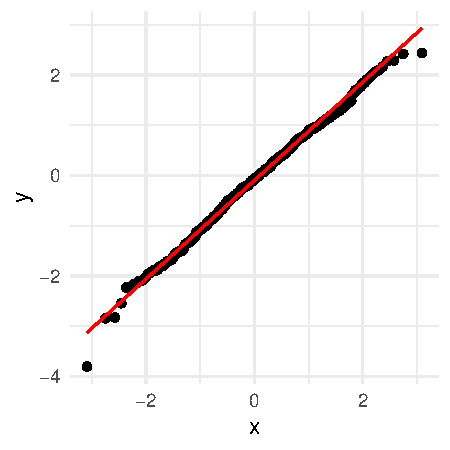
\includegraphics[width=\maxwidth]{img/mc-regression-05-a-1} 

}







\begin{enumerate}
\item [\textbf{A} \msquare] Wir betrachten die Gerade. Wenn die Punkte einigermaßen gleichmäßig um die Gerade verteilt liegen, dann gehen wir von normalverteilten Residuen aus. Dies ist hier nicht der Fall. Wir haben keine normalverteilten Residuen vorliegen.
\item [\textbf{B} \msquare] Wir betrachten die Punkte auf der Geraden. Wenn die Punkte einigermaßen auf der Geraden liegen, dann gehen wir von normalverteilten Residuen aus. Wir können hier von normalverteilten Residuen ausgehen.
\item [\textbf{C} \msquare] Die Annahme der normalverteilten Residuen ist erfüllt. Die Punkte liegen zum überwiegenden Teil nicht auf der Geraden.
\item [\textbf{D} \msquare] Die Annahme der normalverteilten Residuen ist nicht erfüllt. Die Punkte liegen zum überwiegenden Teil nicht auf der Geraden.
\item [\textbf{E} \msquare] Die Annahme der normalverteilten Residuen ist nicht erfüllt. Die Punkte liegen zum überwiegenden Teil auf der Geraden.
\end{enumerate}

\section{Aufgabe \hfill (2 Punkte)}

%% --------------------------------------------------------------------
\ifcollection
\begin{flushright}
\tiny\vspace{-2Ex}
\textbf{\examinhaltstart}
\exammodulestat $\;\bullet$
\exammodulestatbbv $\;\bullet$
\exammodulestatversuch $\;\bullet$
\exammodulebiostat
\vspace{-1Ex}
\end{flushright}
\fi
%% --------------------------------------------------------------------




In den Humanwissenschaften wird der Korrelationskoeffizienten $\rho$ sehr häufig verwendet. Daher ist es auch wichtig für andere Forschende den Korrelationskoeffizienten $\rho$ zu verstehen. Welche Aussazu zu dem Korrelationskoeffizienten $\rho$ ist richtig?




\begin{enumerate}
\item [\textbf{A} \msquare] Der Korrelationskoeffizienten $\rho$ ist eine standardisierte, statistische Maßzahl, die zwischen -1 und 1 liegt. Dabei ist Korrelationskoeffizienten $\rho$ einheitslos.
\item [\textbf{B} \msquare] Der Korrelationskoeffizienten $\rho$ ist eine standardisierte, statistische Maßzahl, die zwischen 0 und 1 liegt. Dabei ist Korrelationskoeffizienten $\rho$ einheitslos. Eine Signifikanz kann nicht nachgewiesen werden.
\item [\textbf{C} \msquare] Der Korrelationskoeffizienten $\rho$ ist eine veraltete Darstellungsform von Effekten in der linearen Regression und wird wie das $\eta^2$ aus der ANOVA interpretiert. Der Korrelationskoeffizienten $\rho$ beschreibt den Anteil an erklärter Varianz durch die Regression.
\item [\textbf{D} \msquare] Korrelationskoeffizienten $\rho$ liegt zwischen 0 und 1. Darüber hinaus ist der Korrelationskoeffizienten $\rho$ einheitslos und kann als Standardisierung verstanden werden.
\item [\textbf{E} \msquare] Der Korrelationskoeffizienten $\rho$ wird wie das $\eta^2$ aus der ANOVA interpretiert. Der Korrelationskoeffizienten $\rho$ beschreibt den Anteil an erklärter Varianz durch die Regression. Dabei gibt er jedoch eine Richtung an und kann auch negativ werden.
\end{enumerate}

\section{Aufgabe \hfill (2 Punkte)}

%% --------------------------------------------------------------------
\ifcollection
\begin{flushright}
\tiny\vspace{-2Ex}
\textbf{\examinhaltstart}
\exammodulestatversuch $\;\bullet$
\exammodulebiostat
\vspace{-1Ex}
\end{flushright}
\fi
%% --------------------------------------------------------------------




Sie rechnen eine linearen Regression und erhalten folgende Abbildung der Residuen (\texttt{.resid}). Welche Aussage ist richtig?



{\centering 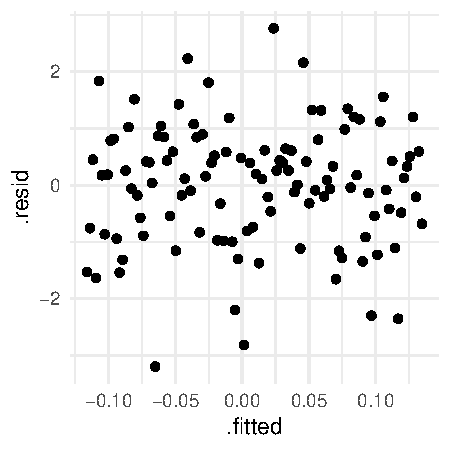
\includegraphics[width=\maxwidth]{img/mc-regression-06-a-1} 

}







\begin{enumerate}
\item [\textbf{A} \msquare] Die Punkte müssen gleichmäßig in dem positiven Bereich liegen. Dies ist hier klar nicht der Fall. Einzelne Ausreißer können beobachtet werden. Die Analyse ist gescheitert.
\item [\textbf{B} \msquare] Die Annahme der normalverteilten Residuen ist nicht erfüllt. Es ist kein Muster zu erkennen.
\item [\textbf{C} \msquare] Die Annahme der normalverteilten Residuen ist erfüllt. Die Punkte liegen zum überwiegenden Teil auf der Diagonalen. Damit ist das Modell erfolgreich geschätzt worden.
\item [\textbf{D} \msquare] Wenn wir die Nulllinie betrachten so liegen die Punkte nicht gleichmäßig über und unter der Nulllinie. Unser Modell erfüllt nicht die Annahme von normalverteilten Residuen mit einem Mittelwert von 0 und einer Streuung von $s^2$.
\item [\textbf{E} \msquare] Die Annahme der normalverteilten Residuen ist erfüllt. Kein Muster ist zu erkennen und keine Outlier zu beobachten.
\end{enumerate}

\section{Aufgabe \hfill (2 Punkte)}

%% --------------------------------------------------------------------
\ifcollection
\begin{flushright}
\tiny\vspace{-2Ex}
\textbf{\examinhaltstart}
\exammodulebiostat
\vspace{-1Ex}
\end{flushright}
\fi
%% --------------------------------------------------------------------




In einer lineren Regression kann es vorkommen, dass der Effekt repräsentiert durch den $\beta$ Koeffizienten nicht so richtig von der Größenordnung zu dem p-Wert passen will. So liefert eine Untersuchung des Einflusses von der $NO_3$-Konzentration in [$\mu g$] im Wasser auf das Trockengewicht in [$kg$] an Erbsen folgende Effekte und p-Werte: $1e-04$ als p-Wert und einen $\beta_{NO_3}$ Koeffizienten von $6.9\times 10^{-7}$. Welche Aussage ist richtig?




\begin{enumerate}
\item [\textbf{A} \msquare] Das Gewicht und die $NO_3$-Konzentration korrelieren sehr stark, deshalb wird der $\beta_{NO_3}$ Koeffizient sehr klein. Mit einer ANOVA kann für die Korrelation korrigiert werden und der Effektschätzer passt dann zum p-Wert.
\item [\textbf{B} \msquare] Manchmal ist die Einheit der Einflussvariable $X$ zu klein gewählt, so dass der Ansteig von 1 Einheit in $X$ zu einer zu kleinen Änderung in $y$ führt. Daher kann der Effekt $\beta_{NO_3}$ sehr klein wirken, aber auf einer anderen Einheit sehr viel größer sein. Der p-Wert wird auf einer einheitslosen Teststatistik bestimmt.
\item [\textbf{C} \msquare] Die Fallzahl ist zu klein angesetzt. Je kleiner die Fallzahl ist, desto höher ist die Teststatsitik und damit auch der $p$-Wert kleiner. Wir brauchen also mehr Fallzahl um den geringen Effekt noch signifikant zu krigen.
\item [\textbf{D} \msquare] Die Einheit der $NO_3$-Konzentration ist zu klein gewählt. Dadurch sehen wir den sehr kleinen $p$-Wert. Der $p$-Wert und die Einheit von der $NO_3$-Konzentration hängen antiproportional zusammen.
\item [\textbf{E} \msquare] Wenn der Effekt $\beta_{NO_3}$ winzig ist, dann kann es an einer falsch gewählten Einheit liegen. Der Anstieg von einer Einheit in $X$ führt ja zu einer Änderung von $\beta_{NO_3}$ in $x$. Wir müssen daher die Einheit von $y$ entsprechend anpassen.
\end{enumerate}

\section{Aufgabe \hfill (2 Punkte)}

%% --------------------------------------------------------------------
\ifcollection
\begin{flushright}
\tiny\vspace{-2Ex}
\textbf{\examinhaltstart}
\exammodulestatversuch $\;\bullet$
\exammodulebiostat
\vspace{-1Ex}
\end{flushright}
\fi
%% --------------------------------------------------------------------




Neben der klassischen Regression kann die Funktion \texttt{lm()} in \Rlogo auch für welche andere Art von Anwendung genutzt werden?





\begin{enumerate}
\item [\textbf{A} \msquare] Neben der klassichen Verwendung der Funktion \texttt{lm()} in der linearen Regression kann auch ein Gruppenvergleich gerechnet werden. Dafür müssen aber alle Faktoren aus den Daten entfernt und numerishc umgewandelt werden. Dann kann das R Paket \{emmeans\} genutzt werden um die Korrelation zu berechnen. Eine Adjustierung ist dann nicht mehr notwendig.
\item [\textbf{B} \msquare] Ist die Einflussvariable $X$ ein Faktor so werden die Gruppenmittelwerte geschätzt und eine anschließende ANOVA sowie multipler Gruppenvergleich mit \{emmeans\} ist möglich. Die Funktion \texttt{lm()} kann dabei eigentlich weggelassen werden, wird aber traditionell gerechnet.
\item [\textbf{C} \msquare] Die Funktion \texttt{lm()} in \Rlogo ist der letzte Schritt für einen Gruppenvergleich. Vorher kann eine ANOVA oder aber ein multipler Vergleich in \{emmeans\} gerechnet werden. In der Funktion  \texttt{lm()} werden die Gruppenvarianzen bestimmt.
\item [\textbf{D} \msquare] Ist die Einflussvariable $X$ numerisch so werden die Gruppenmittelwerte geschätzt und eine anschließende ANOVA sowie multipler Gruppenvergleich mit \{emmeans\} ist möglich.
\item [\textbf{E} \msquare] Ist die Einflussvariable $X$ ein Faktor so werden die Gruppenmittelwerte geschätzt und eine anschließende ANOVA sowie multipler Gruppenvergleich mit \{emmeans\} ist möglich. Dennoch muss zuerst ein lineares Modell mit der Funktion \texttt{lm()} in \Rlogo gerechnet werden.
\end{enumerate}

\section{Aufgabe \hfill (2 Punkte)}

%% --------------------------------------------------------------------
\ifcollection
\begin{flushright}
\tiny\vspace{-2Ex}
\textbf{\examinhaltstart}
\exammodulebiostat
\vspace{-1Ex}
\end{flushright}
\fi
%% --------------------------------------------------------------------




In Ihrer Abschlussarbeit haben Sie neben den klassischen normalverteilten Endpunkte, wie Trockgewicht und Wuchshöhe noch den Infektionsstatus und Zähldaten erhoben. Um diese nicht normalverteilten Endpunkte auszuwerten nutzen Sie das \textit{generalisierte lineare Modell (GLM)}. Welche Aussage ist richtig?




\begin{enumerate}
\item [\textbf{A} \msquare] In \Rlogo ist mit dem \textit{generalisierten linearen Modell (GLM)} eine Modellierung implementiert, die neben der klassischen Normalverteilung auch die Poissonverteilung für Zähldaten oder die Binomialverteilung für 0/1-Daten modellieren kann.
\item [\textbf{B} \msquare] Das GLM ist ein faktisch maschineller Lernalgorithmus, der selstständig die Verteilungsfamilie für Y wählt.
\item [\textbf{C} \msquare] Das GLM ist eine Vereinfachung des LM in R. Mit dem GLM lassen sich polygonale Regressionen rechnen. Somit stehen neben der Normalverteilung noch weitere Verteilungen zu Verfügung.
\item [\textbf{D} \msquare] Das \textit{generalisierte lineare Modell (GLM)} erlaubt auch weitere Verteilungsgruppen für das $X$ bzw. die Einflussvariablen in einer linearen Regression zu wählen.
\item [\textbf{E} \msquare] Das GLM erlaubt auch nicht normalverteilte Residuen in der Schätzung der Regressionsgrade.
\end{enumerate}

\section{Aufgabe \hfill (2 Punkte)}

%% --------------------------------------------------------------------
\ifcollection
\begin{flushright}
\tiny\vspace{-2Ex}
\textbf{\examinhaltstart}
\exammodulebiostat
\vspace{-1Ex}
\end{flushright}
\fi
%% --------------------------------------------------------------------




Neben der Mittelwertsdifferenz als Effektschätzer bei normalverteilten Endpunkten wird auch häufig der Effektschätzer Risk ratio bei binären Endpunkten verwendet. Welche Aussage über den Effektschätzer Risk ratio ist im folgenden Beispiel zur Behandlung von Klaueninfektionen bei Rinder richtig? Dabei sind 5 Tiere krank und 12 Tiere sind gesund.



\begin{enumerate}
\item [\textbf{A} \msquare] Es ergibt sich ein Risk ratio von 2.4, da es sich um ein Anteil handelt.
\item [\textbf{B} \msquare] Da es sich um ein Chancenverhältnis handelt ergibt sich ein Risk ratio von 0.42.
\item [\textbf{C} \msquare] Es ergibt sich ein Risk ratio von 0.42, da es sich um ein Anteil handelt.
\item [\textbf{D} \msquare] Es ergibt sich ein Risk ratio von 0.29, da es sich um eine Chancenverhältnis handelt.
\item [\textbf{E} \msquare] Der Anteil der Kranken wird berechnet. Da es sich um ein Anteil handelt ergibt sich ein Risk ratio von 0.29.
\end{enumerate}
    
% -----------------------------------------------------------------------
\clearpage
% -----------------------------------------------------------------------
\part{Programmieren in R}
% -----------------------------------------------------------------------

\section{Aufgabe \hfill (9 Punkte)}



 
%% --------------------------------------------------------------------
\ifcollection
\begin{flushright}
\tiny\vspace{-3Ex}
\textbf{\examinhaltstart}
\exammodulemathstat $\;\bullet$
\exammodulestat 
\vspace{-4Ex}
\end{flushright}
\begin{minipage}[t]{0.5\textwidth}

\includegraphics[width = 1.3cm]{/Users/kruppajo/work/GitHub/exam/avatare/Jessica.png}
\end{minipage}
\begin{minipage}[t]{0.5\textwidth}
\hfill
\href{https://www.youtube.com/playlist?list=PLe51bCp9JvEFUnFqaJG5aRmON9i1ZbOYC}{
\includegraphics[width = 2cm]{img/youtube}}
\end{minipage}
\vspace{-3ex}
\fi
%% --------------------------------------------------------------------



\ifcollection
\paragraph{Grundlegende Kenntnisse der Programierung in \Rlogo}
\fi

'Hm. \Rlogo ist eigentlich gar nicht so schwer, wenn man die Grundlagen kann.', meint  Jessica ganz zuversichtlich. Nur leider kennt sie sich überhaupt nicht mit \Rlogo aus! Das heißt, Sie müssen hier einmal Rede und Antwort stehen und helfen.\\[1Ex]

Jessica: \textit{Warum gibt es eigentlich Objekte, Wörter und Funktionen in R? Wie unterscheiden sich diese überhaupt?} \textbf{(1 Punkt)}\\[1ex]
Sie antworten:\\[3Ex]

Jessica: \textit{Warum nutzen wir eigentlich dieses \texttt{c()} in \Rlogo?} \textbf{(1 Punkt)}\\[1ex]
Sie antworten:\\[3Ex]

Jessica: \textit{Warum gibt es eigentlich das RStudio und R? Wie unterscheiden sich beide voneinander?} \textbf{(1 Punkt)}\\[1ex]
Sie antworten:\\[3Ex]

Jessica: \textit{Ich habe doch die Spalte mutiert und geändert. Warum sehe ich das in R aber mein Datensatz ändert sich nicht?} \textbf{(1 Punkt)}\\[1ex]
Sie antworten:\\[3Ex]

Jessica: \textit{Wie sieht der Pipe-Operator aus und was ist seine Funktion? Gerne mit Beispiel!} \textbf{(1 Punkt)}\\[1ex]
Sie antworten:\\[3Ex]

Jessica: \textit{Wenn ich was in \Rlogo machen möchte, dann lade ich nochmal welche zwei \Rlogo Pakete sehr häufig?} \textbf{(1 Punkt)}\\[1ex]
Sie antworten:\\[3Ex]

Jessica: \textit{Teilweise brauche ich das Konzept des Faktors in \Rlogo. Was ist ein Faktor?} \textbf{(1 Punkt)}\\[1ex]
Sie antworten:\\[3Ex]

Jessica: \textit{Der Zuweisungs-Operator wird sehr häufig genutzt. Wie sieht der aus und wie funktioniert der an einem Beispiel?} \textbf{(1 Punkt)}\\[1ex]
Sie antworten:\\[3Ex]

Jessica: \textit{Ich habe gehört, dass es Vorteile gibt \Rlogo zu nutzen. Nenne mir mal einen Vorteil!} \textbf{(1 Punkt)}\\[1ex]
Sie antworten:\\[3Ex] 
\clearpage
% -----------------------------------------------------------------------

\section{Aufgabe \hfill (9 Punkte)}



 
%% --------------------------------------------------------------------
\ifcollection
\begin{flushright}
\tiny\vspace{-3Ex}
\textbf{\examinhaltstart}
\exammodulestatversuch $\;\bullet$
\exammodulebiostat
\vspace{-4Ex}
\end{flushright}
\begin{minipage}[t]{0.5\textwidth}

\includegraphics[width = 1.3cm]{/Users/kruppajo/work/GitHub/exam/avatare/Jonas.png}
\end{minipage}
\begin{minipage}[t]{0.5\textwidth}
\hfill
\href{https://www.youtube.com/playlist?list=PLe51bCp9JvEFUnFqaJG5aRmON9i1ZbOYC}{
\includegraphics[width = 2cm]{img/youtube}}
\end{minipage}
\vspace{1ex}
\fi
%% --------------------------------------------------------------------



\ifcollection
\paragraph{Fortgeschrittene Kenntnisse der Programierung in \Rlogo}
\fi

'Hm...am Ende ist dann \Rlogo eigentlich gar nicht so schwer, wenn ich Hilfe habe.', meint  Jonas stolz und lacht Sie an. Nur leider kennt er sich überhaupt nicht mit \Rlogo aus! Das heißt, Sie müssen hier einmal Rede und Antwort stehen und helfen. Sonst wird es für Jonas dann in seinem Projektbericht nichts mit der Auswertung und Abgabe. Das kann auch keine Lösung für Jonas und Sie sein. Immerhin haben Sie schon so viel gelernt.\\[1Ex]

Jonas fragt: \textit{Ich bräuchte mal eine Analogie für das Prinzip von dem r Paket \texttt{\{ggplot\}}. Wie funktioniert das Paket nochmal? So konzeptionell? \textbf{(2 Punkte)}}\\[1ex]
Sie antworten:\\[6.5Ex]

Jonas fragt: \textit{Ich glaube ich habe Varianzheterogenität zwischen den Gruppen vorliegen. Wie funktioniert die Adjustierung dafür nochmal in  \texttt{emmeans()}? \textbf{(1 Punkt)}}\\[1ex]
Sie antworten:\\[6.5Ex]

Jonas fragt: \textit{Nach der EDA zu urteilen liegt eine Interakton vor, wie spezifiziere ich diese im Modell, so dass ich die interaktion zwischen zwei Faktoren $f_1$ und $f_2$ testen kann? \textbf{(1 Punkt)}}\\[1ex]
Sie antworten:\\[6.5Ex]

Jonas fragt: \textit{Ich will eine ANOVA in R rechnen. Dazu brauche ich zwei Funktionen. Welche waren das noch gleich und wie war die Reihenfolge? \textbf{(1 Punkt)}}\\[1ex]
Sie antworten:\\[6.5Ex]

Jonas fragt: \textit{Das Dateiformat in R hat einen Namen. Wie heißt der und gerne mit Beispiel! \textbf{(1 Punkt)}}\\[1ex]
Sie antworten:\\[6.5Ex]

Jonas fragt: \textit{Was muss ich bei der Eingabe eines Datums in Excel beachten, wenn ich später die Exceldatei in R einlesen will? Wie lautet das Format? \textbf{(1 Punkt)}}\\[1ex]
Sie antworten:\\[6.5Ex]

Jonas fragt: \textit{Wie ist noch gleich die Reihenfolge der Funktionen für die Erstellung eines CLD in R. Welche Funktionen brauche ich da? \textbf{(2 Punkte)}}\\[1ex]
Sie antworten:\\[6.5Ex]



 
\clearpage
% -----------------------------------------------------------------------
\part{Deskriptive Statistik \& Explorative Datenanalyse}
% -----------------------------------------------------------------------

\section{Aufgabe \hfill (8 Punkte)}

\textit{Geben Sie grundsätzlich Formeln und Rechenweg zur Lösung der Teilaufgaben mit an!} \\[1Ex]
 

 
%% --------------------------------------------------------------------
\ifcollection
\begin{flushright}
\tiny\vspace{-3Ex}
\textbf{\examinhaltstart}
\exammodulemathstat $\;\bullet$
\exammodulestat $\;\bullet$
\exammodulestatbbv $\;\bullet$
\exammodulestatversuch $\;\bullet$
\exammodulebiostat
\vspace{-4Ex}
\end{flushright}
\begin{minipage}[t]{0.5\textwidth}

\includegraphics[width = 1.3cm]{/Users/kruppajo/work/GitHub/exam/avatare/Tina.png}
\end{minipage}
\begin{minipage}[t]{0.5\textwidth}
\hfill
\href{https://youtu.be/t0WYa_LVc5o}{
\includegraphics[width = 2cm]{img/youtube}}
\end{minipage}
\vspace{-3ex}
\fi
%% --------------------------------------------------------------------



\ifcollection
\paragraph{Zerforschen des Barplots}
\fi

Tina steht vor einem ersten Problem, denn wenn es nach ihrer Betreuer geht, soll sie in einem einem Freilandversuch Brokoli auswertet. Soweit eigentlich alles passend. Besser wäre was anderes gewesen. Tina liebt Astronomie. Darin kann sie sich wirklich verlieren und immer wieder neu begeistern. Das heißt erstmal überlegen für Tina. Aus den Boxen wummert Tocotronic und ihr Mund ist verklebt von Katjes. 'Herrlich', denkt Tina. Die Behandlung werden verschiedene Lichtstufen ($none$, $200lm$ und $600lm$) sein. In ihrer Exceldatei wird sie den Messwert ($Y$) \textit{Frischegewicht} als \textit{freshmatter} aufnehmen. Vorab soll Tina aber eimal die folgenden Barplots ihrer Betreuer nachbauen, damit sie den \Rlogo Code schonmal für später vorliegen hat. Damit geht das Problem schon los. Tina und die Wut, eine unendliche Geschichte mit kniffeligen Wendungen.



{\centering 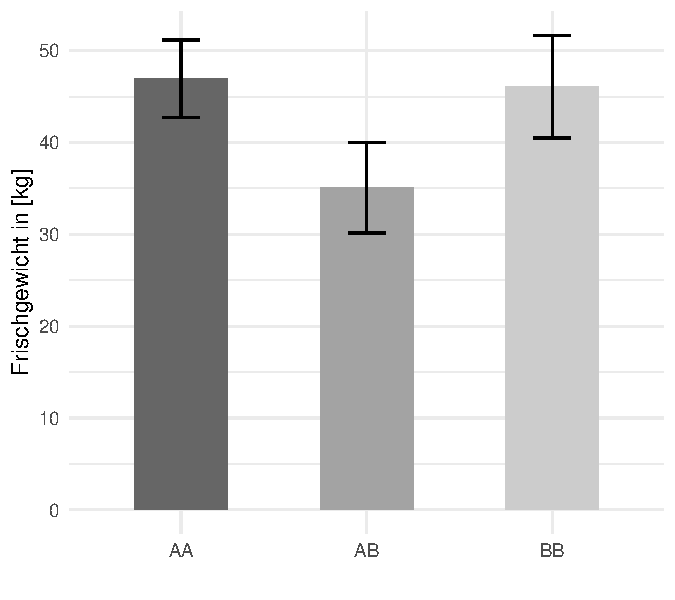
\includegraphics[width=\maxwidth]{img/barplot-02-1} 

}




Leider kennt sich Tina mit der Erstellung von Barplots in \Rlogo nicht aus. Deshalb braucht sie bei der Visualisierung Ihre Hilfe!

\begin{enumerate}
\item Formulieren Sie die wissenschaftliche Fragestellung! \textbf{(1 Punkt)}
\item Erstellen Sie eine Tabelle mit den statistischen Maßzahlen der drei Barplots! \textit{Beachten Sie die korrekte Darstellungsform der statistischen Maßzahlen!} \textbf{(3 Punkte)}
\item Erstellen Sie einen beispielhaften Datensatz im \Rlogo üblichen Format, aus dem die drei Barplots \textit{möglicherweise} erstellt wurden! \textbf{(2 Punkte)}
\item Kann Tina einen Unterschied zwischen den Behandlungen erwarten? Begründen Sie Ihre Antwort! \textbf{(2 Punkte)}
\end{enumerate} 
\clearpage
% -----------------------------------------------------------------------

\section{Aufgabe \hfill (8 Punkte)}

\textit{Geben Sie grundsätzlich Formeln und Rechenweg zur Lösung der Teilaufgaben mit an!} \\[1Ex]
 

 
%% --------------------------------------------------------------------
\ifcollection
\begin{flushright}
\tiny\vspace{-3Ex}
\textbf{\examinhaltstart}
\exammodulemathstat $\;\bullet$
\exammodulestat $\;\bullet$
\exammodulestatbbv 
\vspace{-4Ex}
\end{flushright}
\begin{minipage}[t]{0.5\textwidth}

\includegraphics[width = 1.3cm]{/Users/kruppajo/work/GitHub/exam/avatare/Steffen.png}
\end{minipage}
\begin{minipage}[t]{0.5\textwidth}
\hfill
\href{https://youtu.be/vXnLttRL_VI}{
\includegraphics[width = 2cm]{img/youtube}}
\end{minipage}
\vspace{-3ex}
\fi
%% --------------------------------------------------------------------



\ifcollection
\paragraph{Visualisierung des Barplots}
\fi

Wenn die Romantik nicht wäre, ja dann wäre wohl vieles möglich für Steffen! Aber so.. Deshalb gilt anschauen, was andere vor einem gemacht haben. Für Steffen ist es eine Möglichkeit schneller ans Ziel zu gelangen. Deshalb hat sich Steffen viele Poster in der Fakultät angeschaut und ist zum Schluß gekommen, dass Barplots eine häufig genutzte Abbildung sind. Steffen soll nun in seiner Hausarbeit Kartoffeln untersuchen. Die Behandlung in seiner Hausarbeit sind verschiedene Substrattypen ($torf$, $40p60n$ und $70p30n$). Erhoben wurden von Steffen als Endpunkt ($Y$) \textit{Trockengewicht} benannt als \textit{drymatter} in seiner Exceldatei. Erwartungsgemäß erhält er von seiner Betreuerin den Auftrag die erhobenen Daten als Barplots darzustellen. Dann kann Steffen auch schonmal abschätzen, was bei einem statistischen Test rauskommen könnte. Na dann mal los. Steffen schafft sich die nötige Stimmung. Wenn Taylor Swift ertönt, dann sucht die Schlange schleunigst Schutz unter dem Sofa. Steffen schüttelt den Kopf.

\begin{table}[!h]
\centering
\begin{tabular}{cc}
\toprule
treatment & drymatter\\
\midrule
40p60n & 30.4\\
torf & 42.5\\
torf & 46.0\\
40p60n & 38.4\\
40p60n & 38.1\\
\addlinespace
70p30n & 26.9\\
40p60n & 32.3\\
70p30n & 25.0\\
torf & 48.7\\
70p30n & 22.7\\
\addlinespace
torf & 45.8\\
70p30n & 23.7\\
70p30n & 20.1\\
40p60n & 33.6\\
\bottomrule
\end{tabular}
\end{table}



Leider kennt sich Steffen mit der Erstellung von Barplots nicht aus. Deshalb braucht er bei der Visualisierung Ihre Hilfe!

\begin{enumerate}
\item Formulieren Sie die wissenschaftliche Fragestellung! \textbf{(1 Punkt)}
\item Zeichnen Sie in \textit{einer} Abbildung die Barplots für die Behandlung von Kartoffeln! Beschriften Sie die Achsen entsprechend!\textbf{(4 Punkte)}
\item Beschriften Sie \textit{einen} Barplot mit den gängigen statistischen Maßzahlen! \textbf{(2 Punkte)}
\item Wenn Steffen \textit{keinen Effekt} zwischen den Behandlungen von Kartoffeln erwarten würde, wie sehen dann die Barplots aus? \textit{Antworten Sie mit einer Skizze der Barplots!}
  \textbf{(1 Punkt)}
\end{enumerate} 
\clearpage
% -----------------------------------------------------------------------

\section{Aufgabe \hfill (9 Punkte)}

\textit{Geben Sie grundsätzlich Formeln und Rechenweg zur Lösung der Teilaufgaben mit an!} \\[1Ex]
 

 
%% --------------------------------------------------------------------
\ifcollection
\begin{flushright}
\tiny\vspace{-3Ex}
\textbf{\examinhaltstart}
\exammodulemathstat $\;\bullet$
\exammodulestat $\;\bullet$
\exammodulestatbbv $\;\bullet$
\exammodulestatversuch $\;\bullet$
\exammodulebiostat
\vspace{-4Ex}
\end{flushright}
\begin{minipage}[t]{0.5\textwidth}

\includegraphics[width = 1.3cm]{/Users/kruppajo/work/GitHub/exam/avatare/Steffen.png}
\end{minipage}
\begin{minipage}[t]{0.5\textwidth}
\hfill
\href{https://youtu.be/Xf0yE-o7bEU}{
\includegraphics[width = 2cm]{img/youtube}}
\end{minipage}
\vspace{-3ex}
\fi
%% --------------------------------------------------------------------



\ifcollection
\paragraph{Zerforschen des Boxplots}
\fi

Steffen steht vor einem ersten Problem, denn wenn es nach seinem Betreuer geht, soll er in einem einem Gewächshausexperiment Erbsen auswertet. Soweit eigentlich alles passend. Besser wäre was anderes gewesen. Steffen liebt Klemmbausteine. Darin kann er sich wirklich verlieren und immer wieder neu begeistern. Das heißt erstmal überlegen für Steffen. Steffen schmeißt noch eine Handvoll Oreos in seinen Rachen. Im Hintergrund klirrt leise der Spiegel zum Sound von Taylor Swift. Die Behandlung werden verschiedene Substrattypen ($torf$, $40p60n$ und $70p30n$) sein. In seiner Exceldatei wird er den Messwert ($Y$) \textit{Proteingehalt} als \textit{protein} aufnehmen. Vorab soll Steffen aber eimal die folgenden Boxplots seinem Betreuer nachbauen, damit er den \Rlogo Code schonmal für später vorliegen hat. Damit geht das Problem schon los. Wenn die Romantik nicht wäre, ja dann wäre wohl vieles möglich für Steffen! Aber so..



{\centering 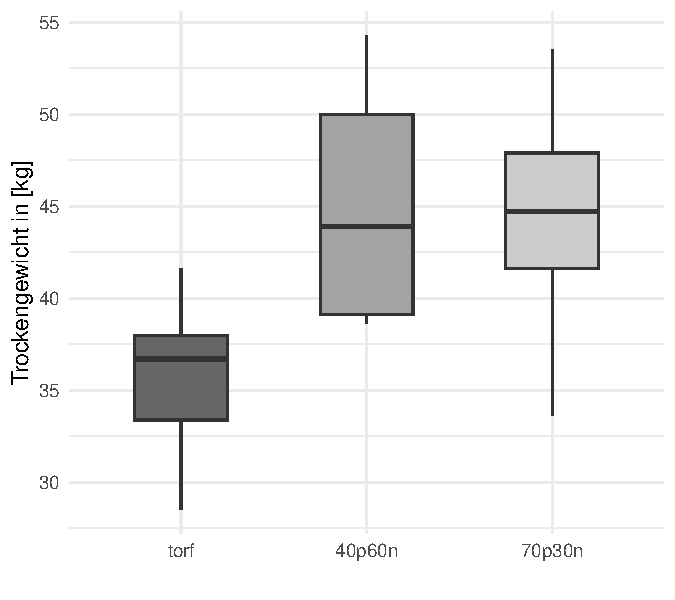
\includegraphics[width=\maxwidth]{img/boxplot-02-zer-1} 

}




Leider kennt sich Steffen mit der Erstellung von Boxplots in \Rlogo nicht aus. Deshalb braucht er bei der Visualisierung Ihre Hilfe!

\begin{enumerate}
\item Erstellen Sie eine Tabelle mit den statistischen Maßzahlen aus der obigen Abbildung der drei Boxplots! \textit{Beachten Sie die korrekte Darstellungsform der statistischen Maßzahlen!} \textbf{(3 Punkte)}
\item Beschriften Sie \textit{einen} der Boxplots mit den gängigen statistischen Maßzahlen! \textbf{(2 Punkte)}
\item Erstellen Sie einen beispielhaften Datensatz, aus dem die drei Boxplots \textit{möglicherweise} erstellt wurden, im \Rlogo üblichen Format! \textbf{(2 Punkte)}
\item Kann Steffen einen Unterschied zwischen den Behandlungen erwarten? Begründen Sie Ihre Antwort! \textbf{(2 Punkte)}
\end{enumerate} 
\clearpage
% -----------------------------------------------------------------------

\section{Aufgabe \hfill (9 Punkte)}

\textit{Geben Sie grundsätzlich Formeln und Rechenweg zur Lösung der Teilaufgaben mit an!} \\[1Ex]
 

 
%% --------------------------------------------------------------------
\ifcollection
\begin{flushright}
\tiny\vspace{-3Ex}
\textbf{\examinhaltstart}
\exammodulemathstat $\;\bullet$
\exammodulestat $\;\bullet$
\exammodulestatbbv 
\vspace{-4Ex}
\end{flushright}
\begin{minipage}[t]{0.5\textwidth}

\includegraphics[width = 1.3cm]{/Users/kruppajo/work/GitHub/exam/avatare/Jonas.png}
\end{minipage}
\begin{minipage}[t]{0.5\textwidth}
\hfill
\href{https://youtu.be/0xc0jIPeiyw}{
\includegraphics[width = 2cm]{img/youtube}}
\end{minipage}
\vspace{-3ex}
\fi
%% --------------------------------------------------------------------



\ifcollection
\paragraph{Visualisierung des Boxplots}
\fi

Boxplots sind bedeutend in der Darstellung von wissenschaftlichen Ergebnissen. Leider hat sich Jonas nicht gemerkt, welche statistischen Maßzahlen für einen Boxplot erhoben werden müssen. Besser wäre was anderes gewesen. Stricken. Ein wunderbares Hobby um sich drin zu verlieren und Abstand zu bekommen. Jonas denkt gerne über Stricken nach. Das ist in soweit doof, da nach seiner Betreuerin nun Boxplots aus seinen Daten gebaut werden sollen, bevor es mit dem statistischen Testen weitergeht. Anhand von Boxplots lässt sich eine Aussage über die Normalverteilung von $Y$ treffen. Die Behandlung für Brokoli waren verschiedene Substrattypen ($torf$ und $70p30n$). Erfasst wurde von Jonas als Messwert ($Y$) \textit{Frischegewicht}. Jonas hat dann \textit{freshmatter} in seiner Exceldatei eintragen. Aber nur in passender Atmospäre! Auf seinem Second Screen läuft Mission Impossible und Jonas schaufelt Snickers. Nicht effizient, aber gut.

\begin{table}[!h]
\centering
\begin{tabular}{cc}
\toprule
treatment & drymatter\\
\midrule
torf & 30.8\\
torf & 37.3\\
torf & 37.8\\
torf & 31.1\\
70p30n & 39.1\\
\addlinespace
torf & 24.8\\
70p30n & 23.9\\
torf & 38.8\\
70p30n & 26.3\\
70p30n & 30.3\\
\addlinespace
70p30n & 31.3\\
torf & 48.9\\
70p30n & 38.5\\
70p30n & 37.6\\
70p30n & 28.9\\
\addlinespace
70p30n & 39.3\\
torf & 32.9\\
torf & 33.7\\
\bottomrule
\end{tabular}
\end{table}



Leider kennt sich Jonas mit der Erstellung von Boxplots nicht aus. Deshalb braucht er bei der Visualisierung Ihre Hilfe!

\begin{enumerate}
\item Zeichnen Sie in \textit{einer} Abbildung die beiden Boxplots für die zwei Behandlungen von Brokoli! Beschriften Sie die Achsen entsprechend! \textbf{(5 Punkte)} 
\item Wie ist Ihr Vorgehen, wenn Sie eine \textit{gerade} Anzahl an
  Beobachtungen pro Gruppe haben? \textbf{(1 Punkt)}
\item Beschriften Sie \textit{einen} der beiden Boxplots mit den gängigen
  statistischen Maßzahlen! \textbf{(2 Punkte)}
\item Wenn Sie \textit{keinen Effekt} zwischen den Behandlungen von
  Brokoli erwarten würden, wie sehen dann die beiden Boxplots aus?
  \textit{Antworten Sie mit einer Skizze der Boxplots!}
  \textbf{(1 Punkt)}
\end{enumerate} 
\clearpage
% -----------------------------------------------------------------------

\section{Aufgabe \hfill (8 Punkte)}

\textit{Geben Sie grundsätzlich Formeln und Rechenweg zur Lösung der Teilaufgaben mit an!} \\[1Ex]
 

 
%% --------------------------------------------------------------------
\ifcollection
\begin{flushright}
\tiny\vspace{-3Ex}
\textbf{\examinhaltstart}
\exammodulestatversuch $\;\bullet$
\exammodulebiostat
\vspace{-4Ex}
\end{flushright}
\begin{minipage}[t]{0.5\textwidth}

\includegraphics[width = 1.3cm]{/Users/kruppajo/work/GitHub/exam/avatare/Nilufar.png}
\end{minipage}
\begin{minipage}[t]{0.5\textwidth}
\hfill
\href{https://youtu.be/aXvxGC4YLqk}{
\includegraphics[width = 2cm]{img/youtube}}
\end{minipage}
\vspace{-3ex}
\fi
%% --------------------------------------------------------------------



\ifcollection
\paragraph{Visualisierung des Histogramm für kategoriale Daten}
\fi

In ihrem Projektbericht möchte Nilufar gerne die Daten aus einem Leistungssteigerungsversuch mit Fleischrindern in einem Histogramm darstellen. Das Histogramm erlaubt ihr dabei Rückschlüsse auf die Verteilung über den Messwert ($Y$) zu treffen. Nilufar schmeißt noch eine Handvoll Takis Blue Heat in ihren Rachen. Im Hintergrund klirrt leise der Spiegel zum Sound von Deichkind. In seinem Experiment hat Nilufar die Anzahl an weißen Blutkörperchen gezählt. Es wäre einfacher, wenn da nicht noch was wäre. Wenn die Erwartung nicht wäre, ja dann wäre wohl vieles möglich für Nilufar! Aber so.. Nilufar nickt im Takt von Deichkind und bemerkt dabei gar nicht was das Huhn schon wieder anstellt.

\begin{center}
Die Anzahl an weißen Blutkörperchen: 8, 4, 5, 7, 2, 3, 4, 2, 2, 4, 3, 7, 4, 4, 6, 5, 3, 4, 4, 8, 3, 7, 2, 4, 4, 4, 6, 6, 3, 4, 3, 7, 3, 5, 2, 5
\end{center}

Leider kennt sich Nilufar mit der Erstellung von Histogrammen überhaupt nicht aus. Deshalb braucht sie bei der Erstellung Ihre Hilfe!

\begin{enumerate}
\item Zeichen Sie ein Histogramm um die Verteilung der Daten zu visualisieren! (\textbf{3 Punkte})
\item Beschriften Sie die Achsen der Abbildung! (\textbf{2 Punkte})
\item Ergänzen Sie die absoluten und relativen Häufigkeiten in der
  Abbildung! \textbf{(1 Punkt)}
\item Berechnen Sie aus den Daten die \textit{Wahrscheinlichkeit}
  mehr als die Anzahl 6 zu beobachten! \textbf{(1
    Punkt)}
\item Berechnen Sie aus den Daten die \textit{Chance} mehr
  als die Anzahl 6 zu beobachten! \textbf{(1 Punkt)}
\end{enumerate}

 
\clearpage
% -----------------------------------------------------------------------

\section{Aufgabe \hfill (8 Punkte)}

\textit{Geben Sie grundsätzlich Formeln und Rechenweg zur Lösung der Teilaufgaben mit an!} \\[1Ex]
 

 
%% --------------------------------------------------------------------
\ifcollection
\begin{flushright}
\tiny\vspace{-3Ex}
\textbf{\examinhaltstart}
\exammodulestatversuch $\;\bullet$
\exammodulebiostat
\vspace{-4Ex}
\end{flushright}
\begin{minipage}[t]{0.5\textwidth}

\includegraphics[width = 1.3cm]{/Users/kruppajo/work/GitHub/exam/avatare/Jessica.png}
\end{minipage}
\begin{minipage}[t]{0.5\textwidth}
\hfill
\href{https://youtu.be/ORHSPTCdfeY}{
\includegraphics[width = 2cm]{img/youtube}}
\end{minipage}
\vspace{-3ex}
\fi
%% --------------------------------------------------------------------



\ifcollection
\paragraph{Visualisierung des Histogramm für kontinuierliche Daten}
\fi

In einem Gespräch mit ihrem Betreuer wird Jessica gebeten seine Daten aus einem Stallexperiment mit Zandern in einem Histogramm darzustellen. 'Hm...', Schokobons und David Bowie. Das ist und bleibt die beste Kombination zum Nachdenken für Jessica. In ihrem Experiment hat er die mittleren dunklen Pigmentstörungen erst fotographiert und dann ausgezählt. Laut ihrem Betreuer soll das Histogramm helfen, die Verteilung der die mittleren dunklen Pigmentstörungen zu bestimmen.  Es wäre einfacher, wenn da nicht noch was wäre. Eine echte Herausforderung für sie war schon immer der Mangel gewesen. Ein leidiges Lied. Wenn David Bowie ertönt, dann sucht die Hündin schleunigst Schutz unter dem Sofa. Jessica schüttelt den Kopf.

\begin{center}
Die mittleren dunklen Pigmentstörungen: 9.4, 8.8, 12.3, 12.2, 12.2, 7.3, 12, 11.5, 8.9, 9.3, 11.3, 9.5, 9.8, 7.8, 11.8, 7.4, 10.2, 8.1, 10, 11.7, 12.3, 11.1, 8.3, 10.6, 14, 5, 9.3, 9
\end{center}

Leider kennt sich Jessica mit der Erstellung von Histogrammen überhaupt nicht aus. Deshalb braucht sie bei der Erstellung Ihre Hilfe!

\begin{enumerate}
\item Zeichen Sie ein Histogramm um die Verteilung der Daten zu visualisieren! (\textbf{3 Punkte})
 \item Erläutern Sie Ihr Vorgehen um ein Histogramm für kontinuierliche Daten zu zeichnen!  (\textbf{2 Punkte})
\item Beschriften Sie die Achsen der Abbildung! (\textbf{2 Punkte})
\item Ergänzen Sie die relativen Häufigkeiten in der Abbildung! \textbf{(1 Punkt)}  
\end{enumerate}

 
\clearpage
% -----------------------------------------------------------------------

\section{Aufgabe \hfill (10 Punkte)}

\textit{Geben Sie grundsätzlich Formeln und Rechenweg zur Lösung der Teilaufgaben mit an!} \\[1Ex]
 

 
%% --------------------------------------------------------------------
\ifcollection
\begin{flushright}
\tiny\vspace{-3Ex}
\textbf{\examinhaltstart}
\exammodulemathstat $\;\bullet$
\exammodulestat $\;\bullet$
\exammodulestatbbv $\;\bullet$
\exammodulestatversuch $\;\bullet$
\exammodulebiostat
\vspace{-4Ex}
\end{flushright}
\begin{minipage}[t]{0.5\textwidth}

\includegraphics[width = 1.3cm]{/Users/kruppajo/work/GitHub/exam/avatare/Steffen.png}
\end{minipage}
\begin{minipage}[t]{0.5\textwidth}
\hfill
\href{https://youtu.be/VAqiUdV4WQ0}{
\includegraphics[width = 2cm]{img/youtube}}
\end{minipage}
\vspace{-3ex}
\fi
%% --------------------------------------------------------------------




\ifcollection
\paragraph{Visualisierung des Scatterplots}
\fi

Steffen schmeißt noch eine Handvoll Oreos in seinen Rachen. Im Hintergrund klirrt leise der Spiegel zum Sound von Taylor Swift. Jetzt heißt es aber erstmal auf was anderes konzentrieren. Steffen möchte gerne den Zusammenhang zwischen mittlerer Eisenkonzentration [Fe/ml] und Protein/Fettrate [\%/kg] im Kontext von Zandern herausfinden. Hierfür hat Steffen ein Stallexperiment im Teuteburgerwald durchgeführt. Nach einigen unvorgesehenen Ereignissen hat er es geschafft folgende Datentabelle zu erstellen. Eine echte Herausforderung für ihn war schon immer die Romantik gewesen. Ein leidiges Lied. Aber das steht auch nicht im Zentrum. Nun stellt sich die Frage für ihn, ob es überhaupt einen Zusammenhang zwischen den gemessenen Variablen gibt. Deshalb möchte Steffen als erstes eine explorative Datenanalyse durchführen. Dann was anderes. Wenn Harry Potter läuft, dann ist die Schlange nicht mehr da. Aber jetzt braucht er mal Entspannung!

\begin{table}[!h]
\centering
\begin{tabular}{cc}
\toprule
Mittlerer Eisenkonzentration [Fe/ml] & Protein/Fettrate [\%/kg]\\
\midrule
10.1 & 16.7\\
18.8 & 25.8\\
18.9 & 25.9\\
16.9 & 22.6\\
11.4 & 23.3\\
\addlinespace
16.4 & 20.9\\
16.4 & 24.0\\
14.7 & 19.9\\
8.6 & 13.0\\
14.9 & 18.8\\
\addlinespace
12.4 & 17.8\\
\bottomrule
\end{tabular}
\end{table}



Leider kennt sich Steffen mit der Erstellung einer explorativen Datenanalyse für kontinuierliche Daten überhaupt nicht aus. Deshalb braucht er bei der Erstellung Ihre Hilfe!

\begin{enumerate}
\item Erstellen Sie eine Visualisierung für die Datentabelle. Beschriften Sie
  die Achsen entsprechend! \textbf{(4 Punkte)}
\item Schätzen Sie eine Gerade durch die Punkte! \textbf{(1 Punkt)}
\item Beschriften Sie die Gerade mit den gängigen statistischen Maßzahlen! Geben Sie die numerischen Zahlenwerte mit an! \textbf{(3 Punkte)}
\item Wenn \textit{kein} Effekt von $x$ auf $y$ vorhanden wäre, wie würde die Gerade verlaufen und welche Werte würden die statistischen Maßzahlen annehmen? \textbf{(2 Punkt)}
\end{enumerate} 
\clearpage
% -----------------------------------------------------------------------

\section{Aufgabe \hfill (10 Punkte)}

\textit{Geben Sie grundsätzlich Formeln und Rechenweg zur Lösung der Teilaufgaben mit an!} \\[1Ex]
 

 
%% --------------------------------------------------------------------
\ifcollection
\begin{flushright}
\tiny\vspace{-3Ex}
\textbf{\examinhaltstart}
\exammodulestat $\;\bullet$
\exammodulestatbbv 
\vspace{-4Ex}
\end{flushright}
\begin{minipage}[t]{0.5\textwidth}

\includegraphics[width = 1.3cm]{/Users/kruppajo/work/GitHub/exam/avatare/Jessica.png}
\end{minipage}
\begin{minipage}[t]{0.5\textwidth}
\hfill
\href{https://youtu.be/t_1KL77mfmg}{
\includegraphics[width = 2cm]{img/youtube}}
\end{minipage}
\vspace{-3ex}
\fi
%% --------------------------------------------------------------------



\ifcollection
\paragraph{Visualisierung des Mosaicplots}
\fi

Zwei kategoriale Variablen darzustellen ist nicht so einfach. Jessica hatte erst über einen Mittelwert nachgedacht, dann aber die Idee verworfen. Wäre da nicht noch was anderes. Wenn der Mangel nicht wäre, ja dann wäre wohl vieles möglich für Jessica! Aber so.. Dabei hatte sie sich in ein Feldexperiment in der Uckermark zum einen die Behandlung Pestizideinsatz [ja/nein] und zum anderen die Messung Trockengewicht über Zielwert [ja/nein] im Kontext von Erdbeeren angeschaut. Jetzt möchte ihre Betreuerin erstmal die langen Tabellen mit ja/nein in einer explorativen Datenanalyse zusammengefasst bekommen. Sonst geht es bei ihrem Projektbericht nicht weiter. Was super nervig ist. Jessica will später nochmal raus um Rad zu fahren. Druck ablassen, dass muss sie auch.



\vspace{1Ex}

\begin{center}
\begin{minipage}[t]{0.45\textwidth}
%\small
\begin{center}

\begin{tabular}{p{2.5cm}p{2.5cm}p{2.5cm}p{2.5cm}}
\toprule
Pestizideinsatz & Trockengewicht über Zielwert\\
\midrule
nein & ja\\
ja & nein\\
nein & ja\\
ja & ja\\
ja & ja\\
\addlinespace
nein & ja\\
ja & ja\\
ja & ja\\
ja & ja\\
ja & ja\\
\addlinespace
nein & ja\\
ja & ja\\
ja & ja\\
nein & ja\\
nein & ja\\
\addlinespace
ja & ja\\
nein & ja\\
\bottomrule
\end{tabular}


\end{center}
\end{minipage}
\begin{minipage}[t]{0.45\textwidth}
%\small
\begin{center}

\begin{tabular}{p{2.5cm}p{2.5cm}p{2.5cm}p{2.5cm}}
\toprule
Pestizideinsatz & Trockengewicht über Zielwert\\
\midrule
nein & ja\\
nein & ja\\
ja & ja\\
ja & ja\\
nein & ja\\
\addlinespace
ja & nein\\
nein & nein\\
ja & ja\\
ja & ja\\
ja & ja\\
\addlinespace
nein & ja\\
ja & ja\\
nein & ja\\
nein & ja\\
nein & ja\\
\addlinespace
ja & ja\\
nein & ja\\
\bottomrule
\end{tabular}


\end{center}
\end{minipage}
\end{center}

\vspace{2Ex}

Leider kennt sich Jessica mit der Erstellung einer explorativen Datenanalyse für kategoriale Daten überhaupt nicht aus. Deshalb braucht sie bei der Erstellung Ihre Hilfe!

\begin{enumerate}
\item Stellen Sie den Zusammenhang zwischen den beiden kategorialen Variablen in einer zusammenfassenden Tabelle dar! \textbf{(3 Punkte)}
\item Visualisieren Sie den Zusammenhang zwischen den beiden kategorialen Variablen! \textbf{(3 Punkte)}
\item Berechnen Sie die Verhältnisse in der Visualisierung! Welche Annahme haben Sie getroffen? \textbf{(2 Punkte)}
\item Wenn \textit{kein} Effekt von der Behandlung vorliegen würde, wie würde die Tabelle und die Visualisierung aussehen? \textbf{(2 Punkt)}
\end{enumerate} 
\clearpage
% -----------------------------------------------------------------------

\section{Aufgabe \hfill (10 Punkte)}

\textit{Geben Sie grundsätzlich Formeln und Rechenweg zur Lösung der Teilaufgaben mit an!} \\[1Ex]
 

 
%% --------------------------------------------------------------------
\ifcollection
\begin{flushright}
\tiny\vspace{-3Ex}
\textbf{\examinhaltstart}
\exammodulestatversuch $\;\bullet$
\exammodulebiostat
\vspace{-4Ex}
\end{flushright}
\begin{minipage}[t]{0.5\textwidth}

\includegraphics[width = 1.3cm]{/Users/kruppajo/work/GitHub/exam/avatare/Alex.png}\hspace{-4mm}
\includegraphics[width = 1.3cm]{/Users/kruppajo/work/GitHub/exam/avatare/Steffen.png}
\end{minipage}
\begin{minipage}[t]{0.5\textwidth}
\hfill
\href{https://youtu.be/Op-gjzASH9I}{
\includegraphics[width = 2cm]{img/youtube}}
\end{minipage}
\fi
%% --------------------------------------------------------------------



\ifcollection
\paragraph{Visualisierung von Verteilungen}
\fi

'Was hast du dir denn da hingeklebt? \textit{Frei ist, wer missfallen kann.}\footnote{Oschmann, A. (2024) Mädchen stärken: Stärken fördern, Selbstwert erhöhen und liebevoll durch Krisen begleiten. Goldegg Verlag}', liest Alex vom Kühlschrank vor. Alex und Steffen sitzen zusammen in der Küche und versuchen zu verhindern, dass die Katze den Biomüll mampft. 'Können wir uns auf die etwas kryptische Aufgabe konzentrieren?', nöhlt Steffen. Die beiden schauen angestrengt auf die drei Boxplots. Das Ziel ist es zu verstehen, wie eine Verteilung anhand eines Boxplots bewertet werden kann. Steffen und die Romantik machen die Sache nicht einfacher.



{\centering 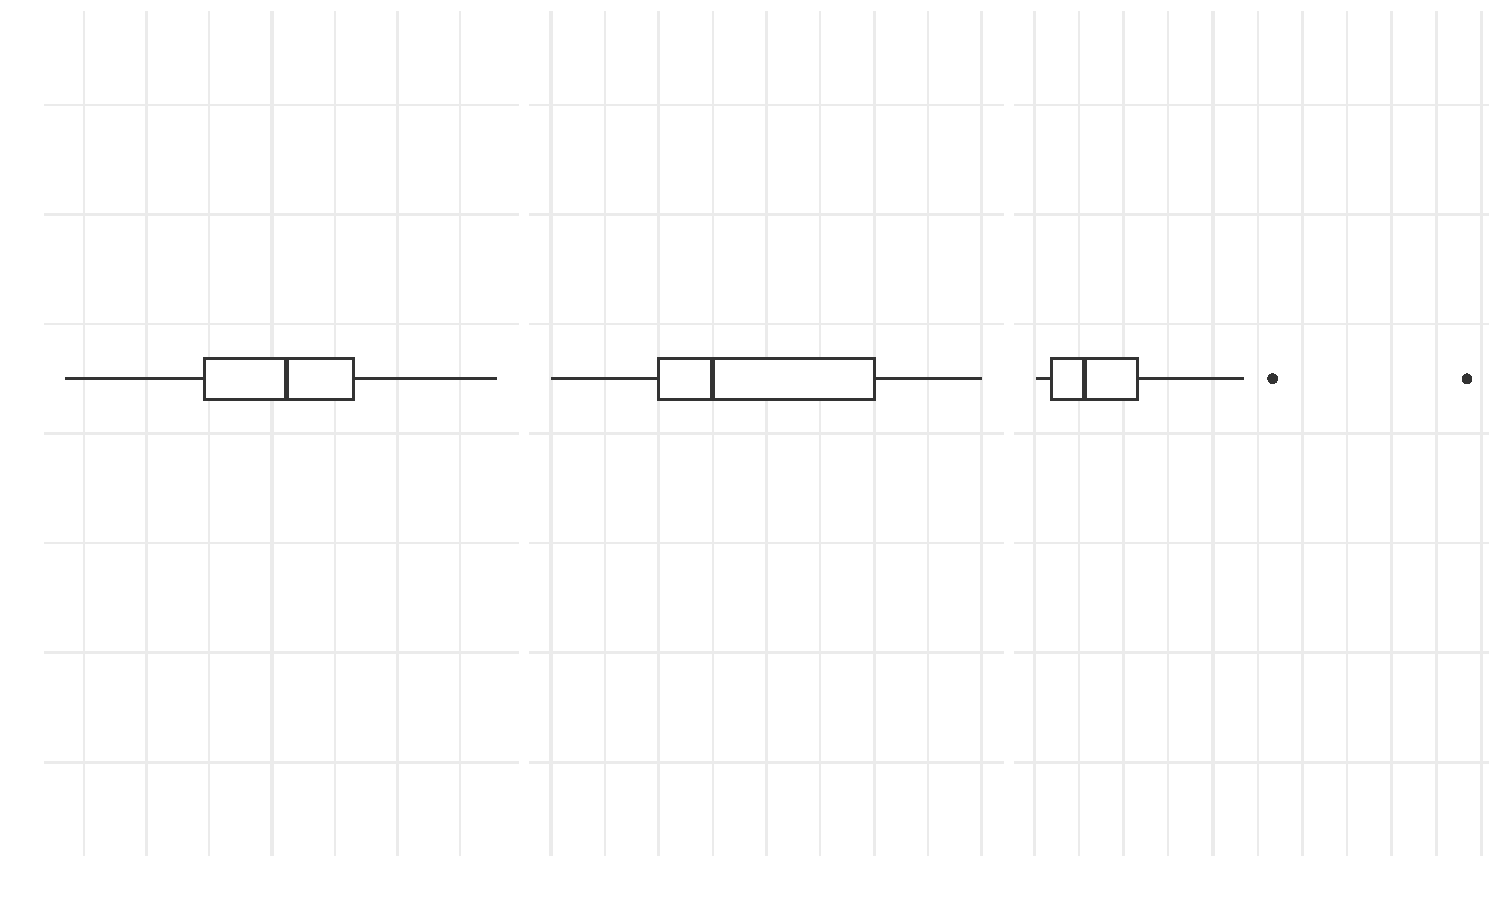
\includegraphics[width=\maxwidth]{img/desc-stat-11-1} 

}




Jetzt brauchen Alex und Steffen Ihre Hilfe bei der Abschätzung einer Verteilung anhand von Boxplots um ihre Arbeit dann in diesem Semester noch abschließen zu können.

\begin{enumerate}
\item Zeichnen Sie über die Boxplots die entsprechende zugehörige Verteilung! \textbf{(3 Punkte)} 
\item Zeichnen Sie unter die Boxplots die entsprechende zugehörige Beobachtungen als Stiche! \textbf{(3 Punkte)}
\item Wie viel Prozent der Beobachtungen fallen in das IQR? Ergänzen Sie die Abbildung entsprechend um den Bereich! \textbf{(2 Punkte)}
\item Wie viel Prozent der Beobachtungen fallen in $\bar{y} \pm 1s$ und $\bar{y} \pm 2s$  unter der Annahme einer Normalverteilung? \textbf{(2 Punkte)}
\end{enumerate} 
\clearpage
% -----------------------------------------------------------------------
\part{Statistisches Testen \& statistische Testtheorie}
% -----------------------------------------------------------------------  

\section{Aufgabe \hfill (9 Punkte)}


 
%% --------------------------------------------------------------------
\ifcollection
\begin{flushright}
\tiny
\textbf{\examinhaltstart}
\exammodulestat $\;\bullet$
\exammodulestatbbv $\;\bullet$
\exammodulestatversuch $\;\bullet$
\exammodulebiostat
\vspace{-4Ex}
\end{flushright}
\begin{minipage}[t]{0.5\textwidth}
\includegraphics[width = 1.3cm]{/Users/kruppajo/work/GitHub/exam/avatare/Paula.png}\hspace{-4mm}\includegraphics[width = 1.3cm]{/Users/kruppajo/work/GitHub/exam/avatare/Yuki.png}
\end{minipage}
\begin{minipage}[t]{0.5\textwidth}
\hfill
\href{https://youtu.be/aHVYuFKTqZs}{\includegraphics[width = 2cm]{img/youtube}}
\end{minipage}
\fi
%% --------------------------------------------------------------------



\ifcollection
\paragraph{Grundgesamtheit und experimentelle Stichprobe}
\fi

'Grundlage des statistischen Testen ist das Verständnis von der Grundgesamtheit (eng. \textit{population} oder \textit{ground truth}) und der experimentellen Stichprobe (eng. \textit{sample}). ', liest Paula laut aus dem Skript vor. Yuki war kurz eingenickt und wird mit einem Stoß geweckt. 'Reiz dich zusammen und iss noch ein paar Smarties das hilft mir immer. Alleine komme ich hier nicht weiter.', tadelt Paula Yuki etwas zu forsch. 'War ne lange Nacht', mault Yuki. Beide sollen in ihrer Abschlussarbeit einen statistischen Test interpretieren und versuchen die Grundlagen zu wiederholen. Yuki war auf einem Konzert von London Grammar.

\vspace{1ex}

Leider kennen sich Paula und Yuki mit der Grundgesamtheit und der Stuchprobe überhaupt nicht aus. Daher sind Sie gefragt!

\begin{enumerate}
\item Nennen Sie das statistische Verfahren und zwei konkrete Beispiele zur Durchführung um von einer Grundgesamtheit auf eine Stichprobe zu gelangen! \textbf{(3 Punkte)}
\item Erklären Sie den Zusammenhang zwischen Stichprobe und Grundgesamtheit an einem Schaubild! Beschriften Sie das Schaubild entsprechend!
  \textit{Nutzen Sie hierfür als Veranschaulichung ein aussagekräftiges Beispiel!}  \textbf{(3 Punkte)}
\item Erweitern Sie das Schaubild um die Entstehung von $Pr(D|H_0)$! \textit{Nutzen Sie hierfür als Veranschaulichung ein aussagekräftiges Beispiel!}  \textbf{(3 Punkte)}
\end{enumerate} 
\clearpage
% -----------------------------------------------------------------------

\section{Aufgabe \hfill (9 Punkte)}


 
%% --------------------------------------------------------------------
\ifcollection
\begin{flushright}
\tiny
\textbf{\examinhaltstart}
\exammodulestat $\;\bullet$
\exammodulestatbbv $\;\bullet$
\exammodulestatversuch $\;\bullet$
\exammodulebiostat
\vspace{-4Ex}
\end{flushright}
\begin{minipage}[t]{0.5\textwidth}
\includegraphics[width = 1.3cm]{/Users/kruppajo/work/GitHub/exam/avatare/Alex.png}\hspace{-4mm}\includegraphics[width = 1.3cm]{/Users/kruppajo/work/GitHub/exam/avatare/Nilufar.png}
\end{minipage}
\begin{minipage}[t]{0.5\textwidth}
\hfill
\href{https://youtu.be/Ric8ne39DtI}{\includegraphics[width = 2cm]{img/youtube}}
\end{minipage}
\fi
%% --------------------------------------------------------------------



\ifcollection
\paragraph{Das Nullritual - Die statistische Testtheorie}
\fi

'Das Känguruh hat mir gerade zugezwinkert. Das macht mir Angst', bemerkt Nilufar. Es reicht ja schon ein Problem. Wenn die Erwartung nicht wäre, ja dann wäre wohl vieles möglich für Nilufar! Aber so.. Da braucht es nicht noch Wahnvorstellungen. 'Ich glaube nicht, das Känguruhs zwinkern. Aber was Wichtigeres. Wo hast du eigentlich meine Schnapspralinen hingetan? Wir haben nur noch Takis Blue Heat von dir. Bäh!', antwortet Alex. Beide sind im Zoo und wollen sich von der statistische Testheorie ablenken lassen. Eigentlich wollte ja Nilufar stoppen wie lange Tiere pinkeln\footnote{Yang, P. J., et al. (2014). Duration of urination does not change with body size. Proceedings of the National Academy of Sciences, 111(33), 11932-11937.}, scheiterte aber an einer Oma mit Stock, die die beiden beschimpfte.

\vspace{1ex}

Leider kennen sich Nilufar und Alex mit statistischen Testtheorie, auch Null-Ritual genannt, überhaupt nicht aus. Geschweige denn mit der Visualisierung als Kreuztabelle.  

\begin{enumerate}
\item Tragen Sie folgende statistische Fachbegriffe zur statistischen Testtheorie korrekt eine selbst erstellte Kreuztabelle ein! \textbf{(3 Punkte)}
  \begin{center}
  \begin{tabular}{cccc}
  $\beta$-Fehler & (Unbekannte) Wahrheit & H$_0$ falsch & 5\% \\
  \end{tabular}
  \end{center}
\item Ergänzen Sie Ihre erstellte Kreuztabelle um vier weitere, passende Fachbegriffe zur statistischen Testtheorie! \textbf{(2 Punkte)}
\end{enumerate}

Die Entscheidungsfindung durch einen statistischen Test kann auch durch die Analogie zu einem Feuermelder abgebildet werden. Dabei symbolisiert der Feuermelder den statistischen Test und es soll getestet werden, ob ein Feuer ausgebrochen ist.

\begin{enumerate}
  \setcounter{enumi}{2}    
\item In der Analogie des Feuermelders, wie lautet der $\alpha$-Fehler? \textbf{(1 Punkt)}
\item In der Analogie des Feuermelders, wie lautet der $\beta$-Fehler? \textbf{(1 Punkt)}
\item Wenn der Feuermelder einmal pro Tag messen würde, wie oft würde der Feuermelder mit einem $\alpha$ von 5\% in einem Monat Alarm schlagen? Begründen Sie Ihre Antwort! \textbf{(2 Punkte)}
\end{enumerate}



 
\clearpage
% -----------------------------------------------------------------------

\section{Aufgabe \hfill (9 Punkte)}

\textit{Geben Sie grundsätzlich Formeln und Rechenweg zur Lösung der Teilaufgaben mit an!} \\[1Ex]


 
%% --------------------------------------------------------------------
\ifcollection
\begin{flushright}
\tiny\vspace{-3Ex}
\textbf{\examinhaltstart}
\exammodulemathstat $\;\bullet$
\exammodulestat $\;\bullet$
\exammodulestatbbv $\;\bullet$
\exammodulestatversuch $\;\bullet$
\exammodulebiostat
\vspace{-4Ex}
\end{flushright}
\begin{minipage}[t]{0.5\textwidth}
\includegraphics[width = 1.3cm]{/Users/kruppajo/work/GitHub/exam/avatare/Jonas.png}\hspace{-4mm}\includegraphics[width = 1.3cm]{/Users/kruppajo/work/GitHub/exam/avatare/Tina.png}
\end{minipage}
\begin{minipage}[t]{0.5\textwidth}
\hfill
\href{https://youtu.be/2LQzyQCy2FI}{\includegraphics[width = 2cm]{img/youtube}}
\end{minipage}
\fi
%% --------------------------------------------------------------------



\ifcollection
\paragraph{Visualisierung der Teststatistik $\boldsymbol{T_D}$ und dem p-Wert}
\fi

'Kannst du mir nochmal an einer Visualisierung erklären, wie der Zusammenhang zwischen der Teststatistik aus den Daten $T_D$ und dem p-Wert ist? Ich habe hier zig Fachbegriffe, kriege die abr nicht zusammen...', fragt Jonas nachdrücklich  Tina. Das hilft aber nur bedingt, denn Tina hat wenig geschlafen und träumt zu den Klängen von Iron Maiden. Jonas hatte den ganzen Abend mit Tina über die Erschöpfung diskutiert und nun sind beide voll neben der Spur. So wird es nichts mit der Klausur. Jonas mampft noch ein paar Snickers und nickt ein. Jetzt brauchen die beiden gesondert Hilfe!

\vspace{1ex}

Leider kennen sich Jonas und Tina mit der Visualisierung der Teststatistik $T_D$ und dem p-Wert überhaupt nicht aus und brauchen dahr Ihre Hilfe!

\vspace{1ex}

\textit{Beachten Sie, dass im Folgenden \underline{keine numerisch korrekte Darstellung} verlangt wird! Es gilt Erkennbarkeit vor Genauigkeit!}

\begin{enumerate}
\item Ergänzen Sie eine beschriftete $x$-Achse! \textbf{(1 Punkt)}
\item Ergänzen Sie "`$\bar{y}_1 = \bar{y}_2$"'! \textbf{(1 Punkt)} 
\item Ergänzen Sie "`$A = 95\%$"'! \textbf{(1 Punkt)}
\item Zeichnen Sie $T_{\alpha=5\%}$ in die Abbildung! \textbf{(1 Punkt)} 
\item Zeichnen Sie das Signifikanzniveau $\alpha$ in die Abbildung! Begründen Sie Ihre Antwort! \textbf{(2 Punkte)} 
\item Zeichnen Sie $+T_{D}$ in die Abbildung! \textbf{(1 Punkt)}
\item Zeichnen Sie einen signifikant p-Wert in die Abbildung! Begründen Sie Ihre Antwort! \textbf{(2 Punkte)}   
\end{enumerate}



{\centering \includegraphics[width=\maxwidth]{img/statistisches-testen-3-1} 

}


 
\clearpage
% -----------------------------------------------------------------------

\section{Aufgabe \hfill (10 Punkte)}


 
%% --------------------------------------------------------------------
\ifcollection
\begin{flushright}
\tiny
\textbf{\examinhaltstart}
\exammodulestatversuch $\;\bullet$
\exammodulebiostat
\vspace{-4Ex}
\end{flushright}
\begin{minipage}[t]{0.5\textwidth}
\includegraphics[width = 1.3cm]{/Users/kruppajo/work/GitHub/exam/avatare/Jonas.png}\hspace{-4mm}\includegraphics[width = 1.3cm]{/Users/kruppajo/work/GitHub/exam/avatare/Mark.png}
\end{minipage}
\begin{minipage}[t]{0.5\textwidth}
\hfill
\href{https://youtu.be/CN_O4fYPbhs}{\includegraphics[width = 2cm]{img/youtube}}
\end{minipage}
\fi
%% --------------------------------------------------------------------



\ifcollection
\paragraph{Visualisierung des 95\% Konfidenzintervalls}
\fi

'So, was haben wir gemacht? Wir haben einen t-test für den Vergleich der Mittelwerte gerechnet.', meint Jonas. Mark schaut fragend. 'Hatten wir nicht alles zu einer Kontrolle verglichen? Das war doch so!', ruft Mark laut aus. 'Wir haben doch als Messwert \textit{Frischegewicht nach Bewässerung} erhoben.', stellt Jonas fest. Jetzt haben beide das Problem, die möglichen 95\% Konfidenzintervalle zu interpretieren.

\vspace{1ex}

Leider kennen sich Jonas und Mark mit der Visualisierung des 95\% Konfidenzintervall überhaupt nicht aus. 

\begin{enumerate}
\item Beschriften Sie die untenstehende Abbildung mit der Signifikanzschwelle! Begründen Sie Ihre Antwort! \textbf{(2 Punkte)}
\item Ergänzen Sie eine \textit{in den Kontext passende} Relevanzschwelle! Begründen Sie Ihre Antwort! \textbf{(2 Punkte)} 
\item Skizieren Sie in die untenstehende Abbildung sechs einzelne Konfidenzintervalle (a-f) mit den
  jeweiligen Eigenschaften! \textbf{(6 Punkte)}
  \begin{itemize}
  \item[(a)] Ein signifikantes, relevantes 95\% Konfidenzintervall 	
  \item[(b)] Ein signifikantes, relevantes 99\% Konfidenzintervall. 	
  \item[(c)] Ein nicht signifikantes, nicht relevantes 95\% Konfidenzintervall 	
  \item[(d)] Ein signifikantes, nicht relevantes 95\% Konfidenzintervall 
  \item[(e)] Ein 95\% Konfidenzintervall mit niedriger Fallzahl $n$ in der Stichprobe als der Rest 95\% der Konfidenzintervalle
  \item[(f)] Ein 95\% Konfidenzintervall mit h{"o}herer Fallzahl $n$ in der Stichprobe als der Rest der 95\% Konfidenzintervalle
  \end{itemize}
\end{enumerate}

\begin{center}
  \includegraphics[height = 10cm]{/Users/kruppajo/work/GitHub/exam/question/img/statistisches-testen-04}
\end{center}


 
\clearpage
% -----------------------------------------------------------------------

\section{Aufgabe \hfill (10 Punkte)}

\textit{Geben Sie grundsätzlich Formeln und Rechenweg zur Lösung der Teilaufgaben mit an!} \\[1Ex]


 
%% --------------------------------------------------------------------
\ifcollection
\begin{flushright}
\tiny\vspace{-3Ex}
\textbf{\examinhaltstart}
\exammodulestatversuch $\;\bullet$
\exammodulebiostat
\vspace{-4Ex}
\end{flushright}
\begin{minipage}[t]{0.5\textwidth}
\includegraphics[width = 1.3cm]{/Users/kruppajo/work/GitHub/exam/avatare/Jessica.png}\hspace{-4mm}\includegraphics[width = 1.3cm]{/Users/kruppajo/work/GitHub/exam/avatare/Jonas.png}
\end{minipage}
\begin{minipage}[t]{0.5\textwidth}
\hfill
\href{https://youtu.be/FgZmpnEWDag}{\includegraphics[width = 2cm]{img/youtube}}
\end{minipage}
\fi
%% --------------------------------------------------------------------



\ifcollection
\paragraph{Zusammenhang zwischen dem Effekt, der Streuung sowie der Fallzahl}
\fi

Es regnet. Wie immer. Aber dafür sind Jessica und Jonas ja auch in Regenbrück zum Lernen verabredet. Gibt es dafür ein besseres Wetter? Eine große Kanne Kaffee und Berge von Schokobons liegen bereit und warten darauf gegessen zu werden. Jessica liest laut vor:\begin{quote}
                 \textit{
                 Beim statistischen Testen gibt es einen Zusammenhang zwischen dem Effekt, der Streuung sowie der Fallzahl. Gegeben sei die Formel für den Student t-Test auf den die folgenden Überlegungen basieren sollen. Welche Auswirkung hat die Änderungen der jeweiligen statistischen Maßzahl des Effekts $\Delta$, der Streuung $s$ und der Fallzahl $n$ auf die Teststistik $T_{D}$, den p-Wert $Pr(D|H_0)$ sowie dem Konfidenzintervall $KI_{1-\alpha}$?
                 }
                 \end{quote}Jonas hebt die Augenbraue. 'Mir ist kalt und es zieht bei dir. Ich bleibe dabei. Wir sollten erstmal Mission Impossible schauen, bis dein Backofen hier mal die küche geheizt hat. Den Film habe ich doch extra mitgebracht! Genauso wie die Pizza!' Jessica ist der Idee nicht abgeneigt und auch die Hündin kommt in die Küche um sich zu wärmen.

\vspace{1ex}

Leider kennen sich Jessica und Jonas mit dem Zusammenhang zwischen dem Effekt, der Streuung sowie der Fallzahl überhaupt nicht aus. 


\begin{enumerate}
\item Visualisieren Sie den Zusammenhang zwischen der Teststatiatik $T_{D}$ und dem p-Wert $Pr(D|H_0)$ für sich verändernde $T_{D}$-Werte!\textit{Geben Sie dafür ein numerisches Beispiel in dem Sie drei $T_{D}$-Werte und deren Einfluss auf den p-Wert vergleichen!} \textbf{(3 Punkte)}  
\item  Füllen Sie die untenstehende Tabelle aus in dem Sie die Änderung der statistischen Maßzahlen auf die Teststatistik, den p-Wert sowie das Konfidenzintervall in \textit{einem} Wort oder Symbol beschreiben! \textbf{(4 Punkte)}
\begin{center}
  \large
  \begin{tabular}[c]{l|c|c|c|l|c|c|c}
    & $T_{D}$ & $Pr(D|H_0)$ & $KI_{1-\alpha}$ & & $T_{D}$ & $Pr(D|H_0)$ & $KI_{1-\alpha}$\strut\\ 
    \hline
    \textbf{$\Delta\; \uparrow$} & \hspace{1.8cm} & \hspace{1.8cm}  & \hspace{1.8cm} & \textbf{
                                                          $\Delta\; \downarrow$} &
                                                                          \hspace{1.8cm} & \hspace{1.8cm}  & \hspace{1.8cm}\strut\\
    \hline
        \textbf{$s\; \uparrow$} & \hspace{1.8cm} & \hspace{1.8cm}  & \hspace{1.8cm} & \textbf{
                                                          $s\; \downarrow$} &
                                                                          \hspace{1.8cm}
                                                & \hspace{1.8cm}  & \hspace{1.8cm}\strut\\
    \hline
        \textbf{$n\; \uparrow$} & \hspace{1.8cm} & \hspace{1.8cm}  & \hspace{1.8cm} & \textbf{
                                                          $n\; \downarrow$} &
                                                                          \hspace{1.8cm}
                                                & \hspace{1.8cm}  & \hspace{1.8cm}\strut\\
    \hline
  \end{tabular}
\end{center}
\item Visualisieren Sie ein 95\%-iges Konfidenzintervall im Vergleich zu einem 99\%-igen Konfidenzintervall! Begründen Sie Ihre Visualisierung anhand der Formel des Konfidenzintervalls des t-Tests mathematisch! \textbf{(3 Punkte)} 
\end{enumerate} 
\clearpage
% -----------------------------------------------------------------------
\part{Der Student t-Test \& Welch t-Test}
% -----------------------------------------------------------------------

\section{Aufgabe \hfill (9 Punkte)}

\textit{Geben Sie grundsätzlich Formeln und Rechenweg zur Lösung der Teilaufgaben mit an!} \\[1Ex]
 

 
%% --------------------------------------------------------------------
\ifcollection
\begin{flushright}
\tiny\vspace{-3Ex}
\textbf{\examinhaltstart}
\exammodulemathstat $\;\bullet$
\exammodulestat $\;\bullet$
\exammodulestatbbv 
\vspace{-4Ex}
\end{flushright}
\begin{minipage}[t]{0.5\textwidth}
\includegraphics[width = 1.3cm]{/Users/kruppajo/work/GitHub/exam/avatare/Alex.png}
\end{minipage}
\begin{minipage}[t]{0.5\textwidth}
\hfill
\href{https://youtu.be/eejS2uG4o-M}{\includegraphics[width = 2cm]{img/youtube}}
\end{minipage}
\vspace{-3ex}
\fi
%% --------------------------------------------------------------------



\ifcollection
\paragraph{Berechnung des Student t-Test \underline{oder} Welch t-Test}
\fi

'Der t-Test testet ein normalverteiltes Outcome ($Y$).', liest Alex laut. Das hilft jetzt auch nur bedingt weiter. Alex und die Gefälligkeit, eine unendliche Geschichte mit kniffeligen Wendungen. Laut seiner Betreuerin ist zwar ihm Messwert Fettgehalt [\%/kg] normalverteilt, aber wie rechnet er jetzt einen t-Test? Für seiner Hausarbeit zum Testen einer neuen technischen Anlage musste er ein Kreuzungsexperiment mit Lamas im Teuteburgerwald durchführen. Als wäre das nicht schon anstrengend genug gewesen bei dem anspruchsvollen Pilotprojekt mit sehr geringer Fallzahl $(n_1 = n_2 = 3)$. Jetzt soll er auch noch testen, ob die Behandlung Lüftungssystem ($keins$ und $vorhanden$) ein signifikantes Ergebnis liefert. Schon dutzende Male gesehen: Alien. Aber immer noch großartig zusammen mit Gummibärchen.

\begin{table}[!h]
\centering
\begin{tabular}{cc}
\toprule
Lüftungssystem & Fettgehalt\\
\midrule
ctrl & 14.4\\
dose & 19.7\\
dose & 18.3\\
ctrl & 16.8\\
ctrl & 15.0\\
\addlinespace
dose & 19.7\\
\bottomrule
\end{tabular}
\end{table}



Leider kennt sich Alex mit der Berechnung eines t-Tests überhaupt nicht aus. Deshalb braucht er bei der Berechnung Ihre Hilfe!

\begin{enumerate}
  \item Formulieren Sie das statistische Hypothesenpaar! \textbf{(1 Punkt)}
  \item Bestimmen Sie die Teststatistik $T_{D}$ eines Welch t-Tests! \textbf{(3 Punkte)}
  \item Treffen Sie mit $T_{\alpha = 5\%} = 2.04$ eine Aussage zur Nullhypothese! Begründen Sie Ihre Antwort! \textbf{(2 Punkte)}
  \item Berechnen Sie den Effekt des Welch t-Tests! \textbf{(1 Punkt)}
  \item Formulieren Sie eine Antwort an Alex über das Ergebnis Ihrer statistischen Analyse! \textbf{(2 Punkte)}
\end{enumerate} 
\clearpage
% -----------------------------------------------------------------------

\section{Aufgabe \hfill (12 Punkte)}

\textit{Geben Sie grundsätzlich Formeln und Rechenweg zur Lösung der Teilaufgaben mit an!} \\[1Ex]
 

 
%% --------------------------------------------------------------------
\ifcollection
\begin{flushright}
\tiny\vspace{-3Ex}
\textbf{\examinhaltstart}
\exammodulemathstat $\;\bullet$
\exammodulestat $\;\bullet$
\exammodulestatbbv 
\vspace{-4Ex}
\end{flushright}
\begin{minipage}[t]{0.5\textwidth}
\includegraphics[width = 1.3cm]{/Users/kruppajo/work/GitHub/exam/avatare/Steffen.png}
\end{minipage}
\begin{minipage}[t]{0.5\textwidth}
\hfill
\href{https://youtu.be/eGoLNgE-WCo}{\includegraphics[width = 2cm]{img/youtube}}
\end{minipage}
\vspace{-3ex}
\fi
%% --------------------------------------------------------------------



\ifcollection
\paragraph{Berechnung des Student t-Test}
\fi

Der Teuteburgerwald, unendliche Weiten. Wir schreiben das Jahr 2024. Dies sind die Abenteuer von Steffen, der mit seiner 1 Mann starken Besatzung 12 Wochen lang unterwegs ist, um neue Welten zu erforschen, neues Leben und neue Zivilisationen. 'Oder nennen wir es Ödnis und Verzweiflung', denkt Steffen. Für seine Abschlussarbeit ist Steffen ins Nichts gezogen. Wenn die Romantik nicht wäre, ja dann wäre wohl vieles möglich für Steffen! Aber so.. Was macht er nun? Steffen hat ein Stallexperiment mit Hühnern durchgeführt. Die Behandlung Bestandsdichte ($Verordnung$ und $Gesteigert$) wurde an Hühnern getestet. Gemessen hat er dann als ein normalverteiltes Outcome ($Y$) Gewichtszuwachs in der 1LW [\%/kg]. Jetzt soll er seinem Betreuer nach testen, ob die Behandlung Bestandsdichte ($Verordnung$ und $Gesteigert$) ein signifikantes Ergebnis liefert. Hm..., was entspannendes wäre gut. Steffen schmeißt noch eine Handvoll Oreos in seinen Rachen. Im Hintergrund klirrt leise der Spiegel zum Sound von Taylor Swift.

\begin{table}[!h]
\centering
\begin{tabular}{cc}
\toprule
Bestandsdichte & Gewichtszuwachs\\
\midrule
Verordnung & 23.0\\
Verordnung & 23.6\\
Gesteigert & 53.2\\
Verordnung & 35.8\\
Verordnung & 11.0\\
\addlinespace
Verordnung & 29.1\\
Gesteigert & 18.5\\
Verordnung & 31.3\\
Verordnung & 32.2\\
Verordnung & 16.8\\
\addlinespace
Gesteigert & 22.9\\
Gesteigert & 37.0\\
Gesteigert & 16.7\\
Verordnung & 28.3\\
Gesteigert & 15.4\\
\addlinespace
Verordnung & 22.1\\
Gesteigert & 41.0\\
Gesteigert & 31.4\\
\bottomrule
\end{tabular}
\end{table}



Leider kennt sich Steffen mit der Berechnung eines t-Tests überhaupt nicht aus. Deshalb braucht er bei der Berechnung Ihre Hilfe!

\begin{enumerate}
  \item Formulieren Sie die wissenschaftliche Fragestellung! \textbf{(1 Punkt)}
  \item Formulieren Sie das statistische Hypothesenpaar! \textbf{(1 Punkt)}
  \item Bestimmen Sie die Teststatistik $T_{D}$ eines Student t-Tests! \textbf{(3 Punkte)}
\item Treffen Sie mit $T_{\alpha = 5\%} = 2.04$ eine Aussage zur Nullhypothese! Begründen Sie Ihre Antwort! \textbf{(2 Punkte)}
\item Berechnen Sie den Effekt des Student t-Tests! \textbf{(1 Punkt)}
\item Wenn Sie \textit{einen} Unterschied zwischen den Behandlungsgruppen erwarten würden, wie groß wäre dann der \textit{mindeste} Effekt? Begründen Sie Ihre Antwort! \textbf{(2 Punkte)}
\item Formulieren Sie eine Antwort an Steffen über das Ergebnis Ihrer statistischen Analyse! \textbf{(2 Punkte)}
\end{enumerate} 
\clearpage
% -----------------------------------------------------------------------

\section{Aufgabe \hfill (12 Punkte)}

\textit{Geben Sie grundsätzlich Formeln und Rechenweg zur Lösung der Teilaufgaben mit an!} \\[1Ex]
 

 
%% --------------------------------------------------------------------
\ifcollection
\begin{flushright}
\tiny\vspace{-3Ex}
\textbf{\examinhaltstart}
\exammodulemathstat $\;\bullet$
\exammodulestat $\;\bullet$
\exammodulestatbbv 
\vspace{-4Ex}
\end{flushright}
\begin{minipage}[t]{0.5\textwidth}
\includegraphics[width = 1.3cm]{/Users/kruppajo/work/GitHub/exam/avatare/Steffen.png}
\end{minipage}
\begin{minipage}[t]{0.5\textwidth}
\hfill
\href{https://youtu.be/TbSEOMCQYl4}{\includegraphics[width = 2cm]{img/youtube}}
\end{minipage}
\vspace{-3ex}
\fi
%% --------------------------------------------------------------------



\ifcollection
\paragraph{Berechnung des Welch t-Test}
\fi


Der t-Test. Steffen erschaudert. Wenn die Romantik nicht wäre, ja dann wäre wohl vieles möglich für Steffen! Aber so.. Ein mächtiges Werkzeug ist der t-Test in den Händen desjenigen, der ein normalverteiltes Outcome ($Y$) hat. Aber erstmal überhaupt den t-Test rechnen können. Wie sah das Experiment von Steffen überhaupt aus? 'Hm...', Oreos und Taylor Swift. Das ist und bleibt die beste Kombination zum Nachdenken für Steffen. Steffen hat ein Gewächshausexperiment mit Brokkoli durchgeführt. Dabei wurde die Behandlung Genotypen ($AA$ und $BB$) an den Brokkoli getestet. Gemessen hat Steffen dann als Messwert Frischegewicht [kg/ha]. Warum der Versuch im Wendland für seinen Projektbericht stattfinden musste, ist ihm bis heute ein Rätsel. Egal. Gibt es jetzt einen Zusammenhang zwischen der Behandlung und Frischegewicht [kg/ha]?

\begin{table}[!h]
\centering
\begin{tabular}{cc}
\toprule
Genotypen & Frischegewicht\\
\midrule
AA & 41.1\\
AA & 47.9\\
BB & 40.4\\
BB & 28.6\\
BB & 35.8\\
\addlinespace
AA & 40.2\\
BB & 32.3\\
BB & 34.7\\
BB & 29.3\\
BB & 27.9\\
\addlinespace
BB & 44.1\\
AA & 58.3\\
AA & 52.9\\
AA & 34.9\\
AA & 62.4\\
\addlinespace
AA & 40.9\\
\bottomrule
\end{tabular}
\end{table}



Leider kennt sich Steffen mit der Berechnung eines t-Tests überhaupt nicht aus. Deshalb braucht er bei der Berechnung Ihre Hilfe!

\begin{enumerate}
  \item Formulieren Sie die wissenschaftliche Fragestellung! \textbf{(1 Punkt)}
  \item Formulieren Sie das statistische Hypothesenpaar! \textbf{(1 Punkt)}
  \item Bestimmen Sie die Teststatistik $T_{D}$ eines  Welch t-Tests! \textbf{(3 Punkte)}
  \item Treffen Sie mit $T_{\alpha = 5\%} = 2.04$ eine Aussage zur Nullhypothese! Begründen Sie Ihre Antwort! \textbf{(2 Punkte)}
\item Berechnen Sie das 99\% Konfidenzintervall. Welche Annahmen haben Sie getroffen? \textbf{(2 Punkte)}
\item Nennen Sie den statistischen Grund, warum Sie sich zwischen einem Student t-Test und einem Welch t-Test entscheiden müssen! \textbf{(1 Punkt)}
\item Formulieren Sie eine Antwort an Steffen über das Ergebnis Ihrer statistischen Analyse! \textbf{(2 Punkte)}
\end{enumerate} 
\clearpage
% -----------------------------------------------------------------------

\section{Aufgabe \hfill (10 Punkte)}

\textit{Geben Sie grundsätzlich Formeln und Rechenweg zur Lösung der Teilaufgaben mit an!} \\[1Ex]
 

 
%% --------------------------------------------------------------------
\ifcollection
\begin{flushright}
\tiny\vspace{-3Ex}
\textbf{\examinhaltstart}
\exammodulemathstat $\;\bullet$
\exammodulestat $\;\bullet$
\exammodulestatbbv $\;\bullet$
\exammodulestatversuch $\;\bullet$
\exammodulebiostat
\vspace{-4Ex}
\end{flushright}
\begin{minipage}[t]{0.5\textwidth}
\includegraphics[width = 1.3cm]{/Users/kruppajo/work/GitHub/exam/avatare/Jessica.png}\hspace{-4mm}\includegraphics[width = 1.3cm]{/Users/kruppajo/work/GitHub/exam/avatare/Nilufar.png}\hspace{-4mm}\includegraphics[width = 1.3cm]{/Users/kruppajo/work/GitHub/exam/avatare/Steffen.png}
\end{minipage}
\begin{minipage}[t]{0.5\textwidth}
\hfill
\href{https://youtu.be/exDo7AyHl4Q}{\includegraphics[width = 2cm]{img/youtube}}
\end{minipage}
\fi
%% --------------------------------------------------------------------



\ifcollection
\paragraph{Interpretation des t-Tests in \Rlogo - die Teststatistik und der p-Wert}
\fi

'Mit dem R Paket \texttt{\{emmeans\}} können wir gleich die Gruppenvergleiche rechnen und uns das \textit{compact letter displac}' ausgeben lassen!', verkündet Steffen sichtlich stolz. Ein paar Mal hat sie schon die Romantik gehindert weiterzumachen. 'Nach Meinung der Betreuerin soll es aber nur erstmal ein t-Test sein. Und die Ausgabe ist schon wirr genug.', merkt Jessica an. Nilufar und Jessica sind bei Steffen um sich in \Rlogo helfen zu lassen. Im Hintergrund wummert Taylor Swift. Jessica streichelt zur Beruhigung die Schlange von Steffen. Die beiden waren 2 Monate im Emsland um einen Versuch mit Erdbeeren in einem Versuch in einer Klimakammer durchzuführen. Ziel war es das Outcome ($Y$) Proteingehalt [g/kg] zu bestimmen. Steffen überlegt, ob er die beiden nicht noch auf den Film \textit{Harry Potter} einlädt oder dann doch lieber raus geht um zu Ringen? Vielleicht will ja Jessica mit. Besser als der Film.

\begin{knitrout}
\definecolor{shadecolor}{rgb}{0.969, 0.969, 0.969}\color{fgcolor}\begin{kframe}
\begin{verbatim}
## 
## 	Two Sample t-test
## 
## data:  Proteingehalt by Genotypen
## t = -6.542, df = 17, p-value = 5.027e-06
## alternative hypothesis: true  is not equal to [condensed]
## 95 percent confidence interval:
##  -14.060614  -7.203023
## sample estimates:
## mean in group AA mean in group BB 
##         35.41818         46.05000
\end{verbatim}
\end{kframe}
\end{knitrout}

Helfen Sie Steffen bei der Interpretation des t-Tests! Sonst geht es auch für Nilufar und Jessica nicht weiter.
  
\begin{enumerate}
  \item Formulieren Sie die wissenschaftliche Fragestellung! \textbf{(1 Punkt)}
  \item Formulieren Sie das statistische Hypothesenpaar! \textbf{(1 Punkt)}
\item Liegt ein signifikanter Unterschied zwischen den Gruppen vor? Begründen Sie Ihre Antwort! \textbf{(2 Punkte)}
\item Skizzieren Sie eine Abbildung in der Sie $T_{D}$, $Pr(D|H_0)$, $A=0.95$, sowie $T_{\alpha=5\%} = |2.11|$ einzeichnen! \textbf{(4 Punkte)}
\item Beschriften Sie die Abbildung! \textbf{(1 Punkt)}  
\item Berechnen Sie den Effekt des t-Tests! \textbf{(1 Punkt)}
\end{enumerate} 
\clearpage
% -----------------------------------------------------------------------

\section{Aufgabe \hfill (10 Punkte)}

\textit{Geben Sie grundsätzlich Formeln und Rechenweg zur Lösung der Teilaufgaben mit an!} \\[1Ex]
 

 
%% --------------------------------------------------------------------
\ifcollection
\begin{flushright}
\tiny\vspace{-3Ex}
\textbf{\examinhaltstart}
\exammodulestatversuch $\;\bullet$
\exammodulebiostat
\vspace{-4Ex}
\end{flushright}
\begin{minipage}[t]{0.5\textwidth}
\includegraphics[width = 1.3cm]{/Users/kruppajo/work/GitHub/exam/avatare/Alex.png}\hspace{-4mm}\includegraphics[width = 1.3cm]{/Users/kruppajo/work/GitHub/exam/avatare/Jessica.png}\hspace{-4mm}\includegraphics[width = 1.3cm]{/Users/kruppajo/work/GitHub/exam/avatare/Steffen.png}
\end{minipage}
\begin{minipage}[t]{0.5\textwidth}
\hfill
\href{https://youtu.be/wJqsNV1hOW8}{\includegraphics[width = 2cm]{img/youtube}}
\end{minipage}
\fi
%% --------------------------------------------------------------------



\ifcollection
\paragraph{Interpretation des t-Tests in \Rlogo - das 95\% Konfidenzintervall}
\fi


'Programmieren ist wie eine Sprache lernen. Man muss es nur machen, dann wird man mit der Zeit immer besser!', gibt Alex zwinkernd zu Protokoll. Ein paar Mal hat sie schon die Gefälligkeit gehindert weiterzumachen. Das hilft jetzt Jessica und Steffen nur bedingt, da beide jetzt die \Rlogo Ausgabe interpretieren müssen und nicht vor drei Wochen, wo noch Zeit gewesen wäre. Beide mampfen konzentriert Schokobons und Oreos in sich hinein. Die beiden hatten im Teuteburgerwald einen Versuch mit Fleischrindern in einem Kreuzungsexperiment durchgeführt. Das war schon anstrengend genug! 'Wir haben Fettgehalt [\%/kg] gemessen, vielleicht hilft das ja...', meint Steffen leicht genervt. Alle starren auf die \Rlogo Ausgabe des t-Tests. Im Hintergrund wummert Abba und man versteht kaum sein eigenes Wort. Steffen hofft, dass die Katze von Alex beruhigend wirkt.

\begin{knitrout}
\definecolor{shadecolor}{rgb}{0.969, 0.969, 0.969}\color{fgcolor}\begin{kframe}
\begin{verbatim}
## 
## 	Two Sample t-test
## 
## data:  Fettgehalt by Bestandsdichte
## t = -1.4963, df = 13, p-value = 0.1584
## alternative hypothesis: true  is not equal to [condensed]
## 95 percent confidence interval:
##  -12.245014   2.223585
## sample estimates:
## mean in group Verordnung mean in group Gesteigert 
##                 34.17500                 39.18571
\end{verbatim}
\end{kframe}
\end{knitrout}

Helfen Sie Alex bei der Interpretation des t-Tests! Sonst geht es auch für Jessica und Steffen nicht weiter.

\begin{enumerate}
  \item Formulieren Sie die wissenschaftliche Fragestellung! \textbf{(1 Punkt)}
  \item Formulieren Sie das statistische Hypothesenpaar! \textbf{(1 Punkt)}
\item Liegt ein signifikanter Unterschied zwischen den Gruppen vor? Begründen Sie Ihre Antwort! \textbf{(2 Punkte)}
\item Skizieren Sie das sich ergebende 95\% Konifidenzintervall! \textbf{(2 Punkte)}
\item Beschriften Sie die Abbildung und das 95\% Konfidenzintervall entsprechend! \textbf{(2 Punkte)}  
\item Interpretieren Sie den Effekt des 95\% Konifidenzintervalls! \textbf{(2 Punkte)}
\end{enumerate} 
\clearpage
% -----------------------------------------------------------------------

\section{Aufgabe \hfill (9 Punkte)}

\textit{Geben Sie grundsätzlich Formeln und Rechenweg zur Lösung der Teilaufgaben mit an!} \\[1Ex]
 

 
%% --------------------------------------------------------------------
\ifcollection
\begin{flushright}
\tiny\vspace{-3Ex}
\textbf{\examinhaltstart}
\exammodulemathstat $\;\bullet$
\exammodulestat $\;\bullet$
\exammodulestatbbv $\;\bullet$
\exammodulestatversuch $\;\bullet$
\exammodulebiostat
\vspace{-4Ex}
\end{flushright}
\begin{minipage}[t]{0.5\textwidth}
\includegraphics[width = 1.3cm]{/Users/kruppajo/work/GitHub/exam/avatare/Alex.png}\hspace{-4mm}\includegraphics[width = 1.3cm]{/Users/kruppajo/work/GitHub/exam/avatare/Mark.png}\hspace{-4mm}\includegraphics[width = 1.3cm]{/Users/kruppajo/work/GitHub/exam/avatare/Nilufar.png}
\end{minipage}
\begin{minipage}[t]{0.5\textwidth}
\hfill
\href{https://youtu.be/w62HJlbN28U}{\includegraphics[width = 2cm]{img/youtube}}
\end{minipage}
\fi
%% --------------------------------------------------------------------



\ifcollection
\paragraph{Interpretation des t-Tests in \Rlogo - die Visualisierung}
\fi

Almería. Spanien. Sonne und Strand. Mark und Alex haben ihren gemeinsamen Auslandsaufenthalt sichtlich genossen. Dann hatte sich auch noch angeboten ihre Abschlussarbeit gemeinsam in Almería durchzuführen. Es hätte sogar noch bessser funktionieret, wenn Nilufar nicht die Erwartung ein paar Mal im Weg gestanden hätte und Mark nicht das Problem gehabt hätte die Unsicherheit zu händeln. Nun müssen jetzt alle Daten in \Rlogo ausgewertet werden, da \Rlogo international der Standard in der Datenauswertung ist und die Betreuer in Spanien nur \Rlogo können. Während beide Nilufar Oliven mit Takis Blue Heat füttern, hoffen Mark und Alex mehr Informationen von Nilufar über die seltsame \Rlogo Ausgabe des t-Tests. Immerhin erinnern beide sich an die Behandlung Ernährungszusatz ($ctrl$ und $fedX$) und das es um Hühnern ging. Im Hintergrund wummert Deichkind und Fotos zeigen Nilufar mit dem Hobby Hip Hop.

\begin{knitrout}
\definecolor{shadecolor}{rgb}{0.969, 0.969, 0.969}\color{fgcolor}\begin{kframe}
\begin{verbatim}
## 
## 	Two Sample t-test
## 
## data:  Schlachtgewicht by Ernährungszusatz
## t = 5.6642, df = 17, p-value = 2.8e-05
## alternative hypothesis: true  is not equal to [condensed]
## 95 percent confidence interval:
##  12.21096 26.70723
## sample estimates:
## mean in group ctrl mean in group fedX 
##           39.35000           19.89091
\end{verbatim}
\end{kframe}
\end{knitrout}

Helfen Sie Nilufar bei der Interpretation des t-Tests! Sonst geht es auch für Mark und Alex nicht weiter.
  
\begin{enumerate}
  \item Formulieren Sie die wissenschaftliche Fragestellung! \textbf{(1 Punkt)}
  \item Formulieren Sie das statistische Hypothesenpaar! \textbf{(1 Punkt)}
\item Liegt ein signifikanter Unterschied zwischen den Gruppen vor? Begründen Sie Ihre Antwort! \textbf{(2 Punkte)}
\item Skizieren Sie die sich ergebenden Boxplot! Welche Annahmen an die Daten haben Sie getroffen? Begründen Sie Ihre
  Antwort! \textbf{(2 Punkte)} 
\item Skizieren Sie die sich ergebenden Barplots! \textbf{(2 Punkte)}
\item Berechnen Sie den Effekt des t-Tests! \textbf{(1 Punkt)}
\end{enumerate}
 
\clearpage
% -----------------------------------------------------------------------
\part{Die einfaktorielle \& zweifaktorielle ANOVA}
% -----------------------------------------------------------------------

\section{Aufgabe \hfill (11 Punkte)}

\textit{Geben Sie grundsätzlich Formeln und Rechenweg zur Lösung der Teilaufgaben mit an!} \\[1Ex]
 

 
%% --------------------------------------------------------------------
\ifcollection
\begin{flushright}
\tiny\vspace{-3Ex}
\textbf{\examinhaltstart}
\exammodulemathstat $\;\bullet$
\exammodulestat $\;\bullet$
\exammodulestatbbv 
\vspace{-4Ex}
\end{flushright}
\begin{minipage}[t]{0.5\textwidth}
\includegraphics[width = 1.3cm]{/Users/kruppajo/work/GitHub/exam/avatare/Paula.png}\hspace{-4mm}\includegraphics[width = 1.3cm]{/Users/kruppajo/work/GitHub/exam/avatare/Tina.png}
\end{minipage}
\begin{minipage}[t]{0.5\textwidth}
\hfill
\href{https://youtu.be/kHmfEmU6lrk}{\includegraphics[width = 2cm]{img/youtube}}
\end{minipage}
\fi
%% --------------------------------------------------------------------



\ifcollection
\paragraph{Visualisierung der einfaktoriellen ANOVA}
\fi

'Uff... die einfaktorielle ANOVA. Und wir können jetzt anhand der Visualisuierung sehen, ob da schon was signifikant ist?', Tina hebt die Augenbraue. 'Ja, können wir. Dafür müssen wir aber erstmal in \texttt{\{ggplot\}} uns die Daten anschauen. Oder wir zeichnen es flott mit der Hand. Geht auch.', meint Paula dazu. Die beiden hatten sich auf einem Konzert von White Lies kennengelernt. Tina hatte sich in ein Gewächshausexperiment verschiedene Lauch angeschaut. Dabei ging es herauszufinden, ob es einen Zusammenhang zwischen der Behandlung Genotypen ($AA$, $AB$ und $BB$) und dem Messwert Chlorophyllgehalt (SPAD-502Plus) [SPAD] gibt. Später wird noch Jagd auf roter Oktober geguckt. Paula befürwortet das!

\begin{knitrout}
\definecolor{shadecolor}{rgb}{0.969, 0.969, 0.969}\color{fgcolor}\begin{table}[!h]
\centering
\begin{tabular}{cc}
\toprule
Genotypen & Chlorophyllgehalt\\
\midrule
BB & 34\\
BB & 35\\
AA & 34\\
AB & 44\\
AB & 44\\
\addlinespace
AA & 34\\
AA & 33\\
BB & 35\\
AB & 45\\
AA & 36\\
\addlinespace
AA & 33\\
BB & 35\\
BB & 35\\
AA & 33\\
AB & 45\\
\addlinespace
BB & 35\\
AB & 45\\
\bottomrule
\end{tabular}
\end{table}

\end{knitrout}

Leider kennen sich Tina und Paula mit Darstellung einer einfaktoriellen ANOVA überhaupt nicht aus. 

\begin{enumerate}
\item Erstellen  Sie  eine  Visualisierung  der  Datentabelle! Beschriften  Sie  die  Abbildung! \textbf{(2 Punkte)}
\item Benennen Sie die Visualisierung mit dem korrekten, statistischen Fachbegriff! \textbf{(1 Punkt)}
\item Zeichnen Sie folgende statistischen Maßzahlen passend ein! 
  \begin{itemize}
  \item Den globalen Mittelwert $\beta_0$ \textbf{(1 Punkt)}
  \item Die Mittelwerte der einzelnen Behandlungsstufen \textbf{(1 Punkt)}
  \item Die Mittelwertsdifferenz der einzelnen Behandlungsstufen mit $\beta_{AA}$, $\beta_{AB}$ und $\beta_{BB}$ \textbf{(1 Punkt)}
  \item Die Residuen oder Fehler mit $\epsilon$ \textbf{(1 Punkt)}
  \end{itemize}
\item Liegt ein \textit{vermutlicher} signifikanter Unterschied vor? Begründen Sie Ihre Antwort! \textbf{(2 Punkte)}
\item Schätzen Sie die Effekte der Behandlungsstufen! \textbf{(2 Punkte)}
\end{enumerate}
 
\clearpage
% -----------------------------------------------------------------------

\section{Aufgabe \hfill (9 Punkte)}

\textit{Geben Sie grundsätzlich Formeln und Rechenweg zur Lösung der Teilaufgaben mit an!} \\[1Ex]
 

 
%% --------------------------------------------------------------------
\ifcollection
\begin{flushright}
\tiny\vspace{-3Ex}
\textbf{\examinhaltstart}
\exammodulemathstat $\;\bullet$
\exammodulestat $\;\bullet$
\exammodulestatbbv 
\vspace{-4Ex}
\end{flushright}
\begin{minipage}[t]{0.5\textwidth}
\includegraphics[width = 1.3cm]{/Users/kruppajo/work/GitHub/exam/avatare/Jessica.png}\hspace{-4mm}\includegraphics[width = 1.3cm]{/Users/kruppajo/work/GitHub/exam/avatare/Paula.png}
\end{minipage}
\begin{minipage}[t]{0.5\textwidth}
\hfill
\href{https://youtu.be/IhecxMcCENY}{\includegraphics[width = 2cm]{img/youtube}}
\end{minipage}
\fi
%% --------------------------------------------------------------------



\ifcollection
\paragraph{Ergebnistabelle der einfaktoriellen ANOVA}
\fi

'Uff... die einfaktorielle ANOVA. Und wie füllen wir jetzt die Tabelle der ANOVA aus und schauen, ob da was signifikant ist?', Jessica hebt die Augenbraue. 'Das ist eine sehr gute Frage. Ich glaube man kann alles in der Tabelle relativ einfach mit wenigen Informationen berechnen.', meint Paula dazu. Da hilft die Ratte von Paula auch nur bedingt. Jessica hatte sich in ein Feldexperiment verschiedene Spargel angeschaut. Dabei ging es herauszufinden, ob es einen Zusammenhang zwischen der Behandlung Bewässerungstypen ($ctrl$, $low$, $mid$ und $high$) und dem Messwert Chlorophyllgehalt (SPAD-502Plus) [SPAD] gibt. Nachher wollen sich beide noch mit dem Hobby Harry Potter von Paula beschäftigen. Kennt Jessica noch nicht, klingt aber interessant.



\vspace{1ex}

Leider kennen sich Jessica und Paula mit Berechnung einer einfaktoriellen ANOVA überhaupt nicht aus. Deshalb brauchen beide bei der Erstellung Ihre Hilfe, die Ratte reicht als Hilfe nicht aus! 

\begin{enumerate}
  \item Formulieren Sie die wissenschaftliche Fragestellung! \textbf{(1 Punkt)}
  \item Formulieren Sie das statistische Hypothesenpaar! \textbf{(1 Punkt)}
\item Füllen Sie die unterstehende einfaktorielle ANOVA Ergebnistabelle aus! \textbf{(3 Punkte)}
\end{enumerate}

\vspace{1Ex}

\begin{center}
  \Large
  \begin{tabular}{lccccp{3cm}}
\toprule
     & \textbf{Df} & \textbf{Sum Sq} & \textbf{Mean Sq} & \textbf{F value} & \textbf{Pr(>F)} \strut\\
    \midrule
   \textbf{Bewässerungstypen}  & 3 &  &  &  &  \strut\\
   \textbf{error}  & 26 & 562.25 &  &  &  \strut\\
   \textbf{Total}  & 29 & 1268.67 &  &  &  \strut\\
\bottomrule
  \end{tabular}
\end{center}

\vspace{1Ex}

\begin{enumerate}
  \setcounter{enumi}{3}
\item Schätzen Sie den p-Wert der Tabelle mit $F_{\alpha = 5\%} = 2.98$ ab. Begründen Sie Ihre Antwort! \textbf{(2 Punkte)}
\item Berechen Sie den Effektschätzer $\eta^2$. Was sagt Ihnen der Wert von $\eta^2$ aus? \textbf{(2 Punkte)}
\end{enumerate}



 
\clearpage
% -----------------------------------------------------------------------

\section{Aufgabe \hfill (12 Punkte)}

\textit{Geben Sie grundsätzlich Formeln und Rechenweg zur Lösung der Teilaufgaben mit an!} \\[1Ex]
 

 
%% --------------------------------------------------------------------
\ifcollection
\begin{flushright}
\tiny\vspace{-3Ex}
\textbf{\examinhaltstart}
\exammodulestatversuch $\;\bullet$
\exammodulebiostat
\vspace{-4Ex}
\end{flushright}
\begin{minipage}[t]{0.5\textwidth}
\includegraphics[width = 1.3cm]{/Users/kruppajo/work/GitHub/exam/avatare/Alex.png}\hspace{-4mm}\includegraphics[width = 1.3cm]{/Users/kruppajo/work/GitHub/exam/avatare/Yuki.png}
\end{minipage}
\begin{minipage}[t]{0.5\textwidth}
\hfill
\href{https://youtu.be/49hvImMwVyE}{\includegraphics[width = 2cm]{img/youtube}}
\end{minipage}
\fi
%% --------------------------------------------------------------------



\ifcollection
\paragraph{Die einfaktoriellen ANOVA und der Student t-Test}
\fi

'Uff... die einfaktorielle ANOVA. Und wie füllen wir jetzt 	extit{genau} die Tabelle der ANOVA aus und schauen, ob da was signifikant ist?', Alex hebt die Augenbraue. 'Das ist eine sehr gute Frage. Ich glaube man kann alles in der Tabelle relativ einfach mit wenigen Informationen berechnen.', meint Yuki dazu und schmiß sich noch ein paar Reese's Peanut Butter Cups in den Rachen. Alex hatte sich in ein Stallexperiment verschiedene Zandern angeschaut. Dabei ging es herauszufinden, ob es einen Zusammenhang zwischen der Behandlung Genotypen ($AA$, $AB$ und $BB$) und dem Messwert Gewichtszuwachs in der 1LW gibt. Nun möchte erstmal seine Betreuerin eine ANOVA Tabelle sehen. Was immer da auch drin zu erkennen sein mag. Später wollen die beiden dann noch raus um zu Boldern.



\vspace{1ex}

Leider kennen sich Alex und Yuki mit Berechnung einer einfaktoriellen ANOVA überhaupt nicht aus. Deshalb brauchen beide bei der Erstellung Ihre Hilfe! 

\begin{enumerate}
  \item Formulieren Sie die wissenschaftliche Fragestellung! \textbf{(1 Punkt)}
  \item Formulieren Sie das statistische Hypothesenpaar! \textbf{(1 Punkt)}
\item Füllen Sie die unterstehende einfaktorielle ANOVA Ergebnistabelle aus! \textbf{(3 Punkte)}
\end{enumerate}

\vspace{1Ex}

\begin{center}
  \Large
  \begin{tabular}{lccccp{3cm}}
\toprule
     & \textbf{Df} & \textbf{Sum Sq} & \textbf{Mean Sq} & \textbf{F value} & \textbf{Pr(>F)} \strut\\
    \midrule
   \textbf{Genotypen}  & 2 & 5301.14 &  &  &  \strut\\
   \textbf{Error}  & 22 & 756.86 &  &  &  \strut\\
\bottomrule
  \end{tabular}
\end{center}

\vspace{1Ex}

\begin{enumerate}
  \setcounter{enumi}{3}
\item Schätzen Sie den p-Wert der Tabelle mit $F_{\alpha = 5\%} = 3.44$ ab. Begründen Sie Ihre Antwort! \textbf{(2 Punkte)}
\item Was bedeutet ein signifikantes Ergebnis in einer einfaktoriellen ANOVA? \textbf{(1 Punkt)}
\item Berechnen Sie \textit{einen} Student t-Test für den \textit{vermutlich} signifikantesten Gruppenvergleich anhand der untenstehenden Tabelle mit $T_{\alpha = 5\%} = 2.03$. Begründen Sie Ihre Auswahl! \textbf{(3 Punkte)}
\end{enumerate}


\begin{knitrout}
\definecolor{shadecolor}{rgb}{0.969, 0.969, 0.969}\color{fgcolor}\begin{table}[!h]
\centering\begingroup\fontsize{11}{13}\selectfont

\begin{tabular}{cccc}
\toprule
\textbf{Genotypen} & \textbf{Fallzahl (n)} & \textbf{Mittelwert} & \textbf{Standardabweichung}\\
\midrule
AA & 9 & 33.00 & 8.12\\
AB & 7 & 1.86 & 3.80\\
BB & 9 & 3.33 & 4.21\\
\bottomrule
\end{tabular}
\endgroup{}
\end{table}

\end{knitrout}


\begin{enumerate}
  \setcounter{enumi}{6}
\item Gegebenen der ANOVA Tabelle war das Ergebnis des Student t-Tests zu erwarten? Begründen Sie Ihre Antwort! \textbf{(2 Punkte)}
\end{enumerate}

 
\clearpage
% -----------------------------------------------------------------------

\section{Aufgabe \hfill (9 Punkte)}

\textit{Geben Sie grundsätzlich Formeln und Rechenweg zur Lösung der Teilaufgaben mit an!} \\[1Ex]
 

 
%% --------------------------------------------------------------------
\ifcollection
\begin{flushright}
\tiny\vspace{-3Ex}
\textbf{\examinhaltstart}
\exammodulemathstat $\;\bullet$
\exammodulestat $\;\bullet$
\exammodulestatbbv
\vspace{-4Ex}
\end{flushright}
\begin{minipage}[t]{0.5\textwidth}
\includegraphics[width = 1.3cm]{/Users/kruppajo/work/GitHub/exam/avatare/Alex.png}
\end{minipage}
\begin{minipage}[t]{0.5\textwidth}
\hfill
\href{https://youtu.be/aXvxGC4YLqk}{\includegraphics[width = 2cm]{img/youtube}}
\end{minipage}
\vspace{-3Ex}
\fi
%% --------------------------------------------------------------------



\ifcollection
\paragraph{Die einfaktorielle ANOVA in \Rlogo}
\fi

'Uff... die einfaktorielle ANOVA und \Rlogo. Nicht so einfach... Was sagt mir jetzt die Ausgabe der ANOVA und wo sehe ich, ob da was signifikant ist?', denkt Alex und hebt die Augenbraue. Alex hatte sich ein Gewächshausexperiment mit Lauch angeschaut. Als wäre das nicht alles schon schwer genug. Eine echte Herausforderung für ihn war schon immer die Gefälligkeit gewesen. Ein leidiges Lied. Dabei ging es beim Experiment herauszufinden, ob es einen Zusammenhang zwischen der Behandlung Düngestufen ($ctrl$, $low$, $mid$ und $high$) und dem Messwert Chlorophyllgehalt (SPAD-502Plus) [SPAD] gibt. Nun möchte sein Betreuer seiner Abschlussarbeit erstmal eine ANOVA sehen und die Ergebnisse präsentiert bekommen. Und eigentlich will er ja was anderes... Schon dutzende Male gesehen: Alien. Aber immer noch großartig zusammen mit Gummibärchen.

\begin{knitrout}
\definecolor{shadecolor}{rgb}{0.969, 0.969, 0.969}\color{fgcolor}\begin{kframe}
\begin{verbatim}
## Analysis of Variance Table
## 
## Response: Chlorophyllgehalt
##             Df Sum Sq Mean Sq F value   Pr(>F)
## Düngestufen  3 233.82  77.940   5.978 0.003858
## Residuals   22 286.83  13.038
\end{verbatim}
\end{kframe}
\end{knitrout}

\vspace{1ex}

Leider kennen sich Alex mit Berechnung einer einfaktoriellen ANOVA überhaupt nicht aus. Deshalb braucht er bei der Erstellung Ihre Hilfe! 

\begin{enumerate}
  \item Formulieren Sie die wissenschaftliche Fragestellung! \textbf{(1 Punkt)}
  \item Formulieren Sie das statistische Hypothesenpaar! \textbf{(1 Punkt)}
\item Interpretieren Sie das Ergebnis der einfaktoriellen ANOVA! \textbf{(2 Punkte)} 
\item Berechnen Sie den Effektschätzer $\eta^2$. Was sagt Ihnen der Wert von $\eta^2$ aus? \textbf{(2 Punkte)}
\item Skizzieren Sie eine Abbildung, der dem obigen Ergebnis der
  einfaktoriellen ANOVA näherungsweise entspricht! \textbf{(3 Punkte)}
\end{enumerate}

 
\clearpage
% -----------------------------------------------------------------------

\section{Aufgabe \hfill (12 Punkte)}

\textit{Geben Sie grundsätzlich Formeln und Rechenweg zur Lösung der Teilaufgaben mit an!} \\[1Ex]
 

 
%% --------------------------------------------------------------------
\ifcollection
\begin{flushright}
\tiny\vspace{-3Ex}
\textbf{\examinhaltstart}
\exammodulestatversuch $\;\bullet$
\exammodulebiostat
\vspace{-4Ex}
\end{flushright}
\begin{minipage}[t]{0.5\textwidth}
\includegraphics[width = 1.3cm]{/Users/kruppajo/work/GitHub/exam/avatare/Paula.png}
\end{minipage}
\begin{minipage}[t]{0.5\textwidth}
\hfill
\href{https://youtu.be/8Pb2sKUIMyk}{\includegraphics[width = 2cm]{img/youtube}}
\end{minipage}
\vspace{-3Ex}
\fi
%% --------------------------------------------------------------------



\ifcollection
\paragraph{Ergebnistabelle der zweifaktoriellen ANOVA}
\fi

In ein Freilandversuch wurden Maiss mit dem Behandlung Lichtstufen ($none$, $200lm$, $400lm$ und $600lm$) sowie der Behandlung Bewässerungstypen ($ctrl$, und $high$) untersucht. Es wurde als Messwert Chlorophyllgehalt (SPAD-502Plus) [SPAD] bestimmt. Paula ahnte schon, dass es komplexer wird, als sie mit ihrer Hausarbeit angefangen hat. Das es jetzt aber so kompliziert wird, hätte sie jetzt aber auch nicht gedacht. Paula kratzt sich am Kopf. Paula mampft aus Frust noch eine Handvoll Smarties. Eventuell muss sie dann doch nochmal Hilfe in der statistischen Beratung holen. Jetzt versucht sie es aber erstmal selber. Und eigentlich wollte Paula doch noch ihrem Hobby nachgehen! Harry Potter. Ein wunderbares Hobby um sich drin zu verlieren und Abstand zu bekommen. Paula denkt gerne über Harry Potter nach.



\vspace{1ex}

Leider kennen sich Paula mit Berechnung einer zweifaktoriellen ANOVA überhaupt nicht aus. Deshalb braucht sie bei der Erstellung Ihre Hilfe! 

\begin{enumerate}
  \item Formulieren Sie die wissenschaftliche Fragestellung! \textbf{(1 Punkt)}
  \item Formulieren Sie das statistische Hypothesenpaar! \textbf{(1 Punkt)}
\item Füllen Sie die unterstehende einfaktorielle ANOVA Ergebnistabelle aus! \textbf{(3 Punkte)}
\end{enumerate}

\vspace{1Ex}

\begin{center}
  \Large
  \begin{tabular}{lccccc}
  \toprule
     & \textbf{Df} & \textbf{Sum Sq} & \textbf{Mean Sq} & \textbf{F value} & \textbf{Pr(>F)} \strut\\
    \midrule
   \textbf{Lichtstufen}  & 3 & 398.33 &  &  &  \strut\\
    \textbf{Bewässerungstypen}  & 1 & 131.13 &  &  &  \strut\\
    \textbf{Lichtstufen:Bewässerungstypen}  & 3 & 39.32 &  &  &  \strut\\
   \textbf{Error}  & 18 & 359.86 &  &  &  \strut\\
\bottomrule
  \end{tabular}
\end{center}

\vspace{1Ex}

\begin{enumerate}
  \setcounter{enumi}{3}
\item Schätzen Sie den p-Wert der Tabelle ab. Begründen Sie Ihre
  Antwort! \textbf{(3 Punkte)}
\end{enumerate}
  
\begin{center}
    \Large
\begin{tabular}{lc}
  \toprule
     & $\boldsymbol{F_{\alpha = 5\%}}$ \\
\midrule
  \textbf{Lichtstufen} & $4.26$ \\
  \textbf{Bewässerungstypen} & $3.40$ \\
  \textbf{Lichtstufen:Bewässerungstypen} & $5.23$ \\
  \bottomrule
  \end{tabular}
\end{center}

\begin{enumerate}
  \setcounter{enumi}{4}
\item Was bedeutet ein signifikantes Ergebnis in einer zweifaktoriellen ANOVA? \textbf{(2 Punkte)}
\item Was sagt der Term \textit{Lichtstufen:Bewässerungstypen} aus? Interpretieren Sie das Ergebnis! \textbf{(2 Punkte)}
\end{enumerate}
 
\clearpage
% -----------------------------------------------------------------------

\section{Aufgabe \hfill (10 Punkte)}

\textit{Geben Sie grundsätzlich Formeln und Rechenweg zur Lösung der Teilaufgaben mit an!} \\[1Ex]
 

 
%% --------------------------------------------------------------------
\ifcollection
\begin{flushright}
\tiny\vspace{-3Ex}
\textbf{\examinhaltstart}
\exammodulestatversuch $\;\bullet$
\exammodulebiostat
\vspace{-4Ex}
\end{flushright}
\begin{minipage}[t]{0.5\textwidth}
\includegraphics[width = 1.3cm]{/Users/kruppajo/work/GitHub/exam/avatare/Mark.png}
\end{minipage}
\begin{minipage}[t]{0.5\textwidth}
\hfill
\href{https://youtu.be/rWTyHXXlYjY}{\includegraphics[width = 2cm]{img/youtube}}
\end{minipage}
\vspace{-3Ex}
\fi
%% --------------------------------------------------------------------



\ifcollection
\paragraph{Die zweifaktorielle ANOVA in \Rlogo}
\fi

In ein Kreuzungsexperiment wurden Fleischrindern mit der Behandlung Lüftungssystem ($keins$, $storm$, $tornado$ und $thunder$) sowie der Behandlung Genotypen ($AA$ und $BB$) untersucht. Es wurde als Messwert Fettgehalt [\%/kg] bestimmt. Jetzt starrt Mark mit auf die \Rlogo Ausgabe einer zweifaktoriellen ANOVA. Leider starrt sein Betreuer in der gleichen Art Mark zurück an. Das wird ein langer Nachmmittag, denkt er sich und kreuselt seinen Mund. 'Und was machen wir jetzt?' entfährt es ihm überrascht entnervt. Immerhin war geht es ja um der Projektbericht. Mark hätte doch nichts mit Fleischrindern machen sollen. Fleischrindern -- was soll das auch bedeutendes sein? Eigentlich wollte Mark nachher noch einen Film schauen. Das Verrückte ist, dass der Hamster Columbo wirklich liebt. Das ist Mark sehr recht, denn er braucht Entspannung.

\begin{knitrout}
\definecolor{shadecolor}{rgb}{0.969, 0.969, 0.969}\color{fgcolor}\begin{kframe}
\begin{verbatim}
## Analysis of Variance Table
## 
## Response: Fettgehalt
##                          Df Sum Sq Mean Sq F value  Pr(>F)
## Lüftungssystem            2 154.69  77.346  3.0792 0.07077
## Genotypen                 1 101.93 101.929  4.0578 0.05916
## Lüftungssystem:Genotypen  2 277.49 138.743  5.5234 0.01348
## Residuals                18 452.15  25.119
\end{verbatim}
\end{kframe}
\end{knitrout}

\vspace{1ex}

Leider kennt sich Mark mit Berechnung einer zweifaktoriellen ANOVA überhaupt nicht aus. Deshalb braucht er bei der Erstellung Ihre Hilfe! 

\begin{enumerate}
  \item Formulieren Sie die wissenschaftliche Fragestellung! \textbf{(1 Punkt)}
  \item Formulieren Sie das statistische Hypothesenpaar! \textbf{(1 Punkt)}
\item Interpretieren Sie das Ergebnis der einfaktoriellen ANOVA! \textbf{(3 Punkte)} 
\item Zeichnen Sie eine Abbildung, der dem obigen Ergebnis der
  zweifaktoriellen ANOVA näherungsweise entspricht! \textbf{(5 Punkte)}
\end{enumerate}
 
\clearpage
% -----------------------------------------------------------------------

\section{Aufgabe \hfill (11 Punkte)}

\textit{Geben Sie grundsätzlich Formeln und Rechenweg zur Lösung der Teilaufgaben mit an!} \\[1Ex]
 

 
%% --------------------------------------------------------------------
\ifcollection
\begin{flushright}
\tiny\vspace{-3Ex}
\textbf{\examinhaltstart}
\exammodulestatversuch $\;\bullet$
\exammodulebiostat
\vspace{-4Ex}
\end{flushright}
\begin{minipage}[t]{0.5\textwidth}
\includegraphics[width = 1.3cm]{/Users/kruppajo/work/GitHub/exam/avatare/Mark.png}
\end{minipage}
\begin{minipage}[t]{0.5\textwidth}
\hfill
\href{https://youtu.be/2qG1Dws0MJo}{\includegraphics[width = 2cm]{img/youtube}}
\end{minipage}
\vspace{-3Ex}
\fi
%% --------------------------------------------------------------------



\ifcollection
\paragraph{Interaktion in der zweifaktoriellen ANOVA}
\fi

In ein Kreuzungsexperiment wurden Fleischrindern mit der Behandlung Bestandsdichte ($standard$, $eng$, $weit$ und $kontakt$) sowie der Behandlung Genotypen ($AA$ und $BB$) untersucht. Es wurde als Messwert Gewichtszuwachs in der 1LW bestimmt. Jetzt starrt Mark mit auf die \Rlogo Ausgabe einer zweifaktoriellen ANOVA. Leider starrt sein Betreuer in der gleichen Art Mark zurück an. Es liegt anscheinend eine signifikante Interaktion vor? 'Das wird ein langer Nachmmittag.', denkt er sich und kreuselt seinen Mund. 'Und was machen wir jetzt?' entfährt es ihm überrascht entnervt. Immerhin war geht es ja um der Projektbericht. Mark hätte doch nichts mit Fleischrindern machen sollen. Fleischrindern -- was soll das auch bedeutendes sein? Eigentlich wollte Mark nachher noch einen Film schauen. Wenn Columbo läuft, dann ist der Hamster nicht mehr da. Aber jetzt braucht er mal Entspannung!

\vspace{1ex}

Leider kennen sich Mark und sein Betreuer mit der zweifaktoriellen ANOVA überhaupt nicht aus. Geschweige denn mit der Interpretation einer Interaktion. Deshalb braucht er bei der Erstellung Ihre Hilfe, sonst wird es heute Abend mit seinem Hobby Geocaching nichts mehr! 

\begin{enumerate}
\item Visualisieren Sie folgende mögliche Interaktionen zwischen den Behandlungen! Beschriften Sie die Abbildung! \textbf{(4 Punkte)}
\begin{enumerate}
\item \underline{Keine} Interaktion liegt vor.
\item Eine \underline{schwache} Interaktion liegt vor. 
\item Eine \underline{starke} Interaktion liegt vor. 
\end{enumerate}
\item Erklären Sie den Unterschied zwischen den verschiedenen Interaktionen! \textbf{(2 Punkte)}
\item Welche statistische Maßzahl betrachten Sie für die Bewertung der Interaktion? \textbf{(1 Punkt)}
\item Skizzieren Sie die notwendigen Funktionen in \Rlogo für eine Post-hoc Analyse! \textbf{(2 Punkte)} 
\item Wenn eine signifikante Interaktion in den Daten vorliegt, wie ist dann das weitere Vorgehen? Berücksichtigen Sie auch die Funktion \texttt{emmeans()}! \textbf{(2 Punkte)}
\end{enumerate}

 
\clearpage
% -----------------------------------------------------------------------

\section{Aufgabe \hfill (12 Punkte)}

\textit{Geben Sie grundsätzlich Formeln und Rechenweg zur Lösung der Teilaufgaben mit an!} \\[1Ex]
 

 
%% --------------------------------------------------------------------
\ifcollection
\begin{flushright}
\tiny\vspace{-3Ex}
\textbf{\examinhaltstart}
\exammodulebiostat
\vspace{-4Ex}
\end{flushright}
\begin{minipage}[t]{0.5\textwidth}
\includegraphics[width = 1.3cm]{/Users/kruppajo/work/GitHub/exam/avatare/Jonas.png}
\end{minipage}
\begin{minipage}[t]{0.5\textwidth}
\hfill
\href{https://youtu.be/FjjJXkFJfIY}{\includegraphics[width = 2cm]{img/youtube}}
\end{minipage}
\vspace{-3Ex}
\fi
%% --------------------------------------------------------------------



\ifcollection
\paragraph{Zusammenhang zwischen der ANOVA und dem t-Test}
\fi

In ein Freilandversuch wurden Brokkoli mit der Behandlung Genotypen ($AA$, $AB$ und $BB$) sowie der Behandlung Bewässerungstypen ($ctrl$, und $high$) untersucht. Jonas schaut konzentriert auf die Formeln der ANOVA und des t-Tests. In seinem Experiment wurde als Messwert Proteingehalt [g/kg] bestimmt. Wenn die Erschöpfung nicht wäre, ja dann wäre wohl vieles möglich für Jonas! Aber so.. Dann wäre es nicht noch komplizierter. Was war da jetzt nochmal der Zusammenhang zwischen den beiden statistischen Verfahren? Beide Verfahren haben ja irgendwie etwas miteinander zu tun und sein Betreuer möchte das jetzt auch noch verstehen. Muss das nicht eigentlich klar sein? Immerhin ist Jonas nicht die erste Betreuung eines Projektberichts. Immerhin hat er die beiden Formeln vorliegen. Schon dutzende Male gesehen: Mission Impossible. Aber immer noch großartig zusammen mit Snickers.

\begin{graybox}{Gegebene Formeln}
\begin{center}
  \begin{tabular}{cc}
    $F_{D} = \cfrac{MS_{treatment}}{MS_{error}}$ & $T_{D} = \cfrac{\bar{y}_1 - \bar{y}_2}{s_p \cdot \sqrt{2/n_g}}$\\
  \end{tabular}
\end{center}
\end{graybox}

Leider kennen sich Jonas mit dem Zusammenhang zwischen der ANOVA und dem t-Test nicht aus. Deshalb braucht er bei der Erstellung Ihre Hilfe! 

\begin{enumerate}
\item Welche statistische Maßzahl testet der t-Test, welche die ANOVA? Begründen Sie Ihre Antwort! \textbf{(2 Punkte)}
\item Erklären Sie den Zusammenhang zwischen der $F_{D}$ Statistik und $T_{D}$ Statistik! \textbf{(2 Punkte)}
\item Visualisieren Sie in einer 2x2 Tafel den Zusammenhang von $MS_{treatment}$ und $MS_{error}$! \textbf{(2 Punkte)}
\item Beschriften Sie die erstellte 2x2 Tafel mit \underline{signifikant} und \underline{nicht signifikant}! Begründen Sie Ihre Antwort! \textbf{(2 Punkte)}
\item Nennen Sie das numerische Minimum der F-Statistik $F_D$! Begründen Sie Ihre Antwort! \textbf{(2 Punkte)}
\item Wenn die F-Statistik $F_D$ minimal ist, welche Aussage erhalten Sie über die Nullhypothese? Begründen Sie Ihre Antwort! \textbf{(2 Punkte)}
\end{enumerate}

 
\clearpage
% -----------------------------------------------------------------------

\section{Aufgabe \hfill (11 Punkte)}

\textit{Geben Sie grundsätzlich Formeln und Rechenweg zur Lösung der Teilaufgaben mit an!} \\[1Ex]
 

 
%% --------------------------------------------------------------------
\ifcollection
\begin{flushright}
\tiny\vspace{-3Ex}
\textbf{\examinhaltstart}
\exammodulebiostat
\vspace{-4Ex}
\end{flushright}
\begin{minipage}[t]{0.5\textwidth}
\includegraphics[width = 1.3cm]{/Users/kruppajo/work/GitHub/exam/avatare/Jonas.png}
\end{minipage}
\begin{minipage}[t]{0.5\textwidth}
\hfill
\href{https://youtu.be/M9Uhm67ndxM}{\includegraphics[width = 2cm]{img/youtube}}
\end{minipage}
\vspace{-3Ex}
\fi
%% --------------------------------------------------------------------



\ifcollection
\paragraph{Zusammenhang zwischen der ANOVA und dem Post-hoc-Test}
\fi

In einen Leistungssteigerungsversuch wurden die Daten $D$ von Puten mit der Behandlung Genotypen ($AA$, $AB$ und $BB$) untersucht. Es wurde als Messwert Protein/Fettrate [\%/kg] bestimmt. Jetzt starrt Jonas mit auf die \Rlogo Ausgabe einer einfaktoriellen ANOVA. Anscheinend gibt es ein Problem mit der Annahme der Normalverteilung und der Varianzhomogenität der ANOVA in den Daten. 'Wir haben jetzt bei der ANOVA einen p-Wert mit 0.061 raus sowie eine F-Statistik $F_D$ mit 1.2 berechnet. Nach den Boxplots müsste sich eigentlich ein Unterschied zwischen $AA$ und $BB$ ergeben. Der Unterschied ist in \texttt{\{emmeans\}} auch signifikant mit einem p-Wert von 0.021. Wie kann das sein?', meint Jonas ungläubig. Leider starrt seine Betreuerin in der gleichen Art Jonas zurück an. Jonas hat schon genug Probleme. Wenn die Erschöpfung nicht wäre, dann wäre es einfacher. Das wird ein langer Nachmmittag, denkt er sich und kreuselt seinen Mund. 'Und was machen wir jetzt?' entfährt es ihm überrascht entnervt. Immerhin war geht es ja um seine Hausarbeit. Jonas hätte doch nichts mit Puten machen sollen. Puten -- was soll das auch bedeutendes sein? Hoffentlich kommt er noch zum Konzert von Iron Maiden. Nervös krault er das Meerschweinchen.

\begin{graybox}{Gegebene Formeln}
\begin{center}
  \begin{tabular}{ccc}
    $MS_{treatment} = \cfrac{SS_{treatment}}{df_{treatment}}$ &
    $MS_{error} = \cfrac{SS_{error}}{df_{error}}$ &
    $F_{D} = \cfrac{MS_{treatment}}{MS_{error}}$ \\
  \end{tabular}
\end{center}
\end{graybox}

Leider kennen sich Jonas und seine Betreuerin mit der Interpretation einer ANOVA überhaupt nicht aus. Deshalb braucht er bei der Erstellung Ihre Hilfe und die Zeit wird knapp. 

\begin{enumerate}
  \item Formulieren Sie die wissenschaftliche Fragestellung! \textbf{(1 Punkt)}
  \item Formulieren Sie das statistische Hypothesenpaar! \textbf{(1 Punkt)}
\item Was bedeutet eine signifkante ANOVA für die beobachteten Daten $D$? \textbf{(1 Punkt)}
\item Visualisieren Sie den Unterschied zwischen Varianzhomogenität und Varianzheterogenität anhand der Daten $D$! Beschriften Sie die Abbildung! \textbf{(2 Punkte)} 
\item Visualisieren Sie für die Daten $D$ die Verletzung der Annahme der Varianzhomogenität der ANOVA unter zu Hilfenahme von Boxplots! Beschriften Sie die Abbildung! \textbf{(2 Punkte)}
\item Welche Auswirkung hat die Verletzung der Annahme der Varianzhomogenität für die Teststatistik $F_D$ der ANOVA? Begründen Sie Ihre Antwort! \textbf{(2 Punkte)}
\item Erklären Sie abschließend die Diskrepanz zwischen den Ergebnis der ANOVA und dem paarweisen Gruppenvergleich in \texttt{\{emmeans\}}! \textbf{(2 Punkte)}
\end{enumerate}

 
\clearpage
% -----------------------------------------------------------------------
\part{Multiple Gruppenvergleiche}
% ----------------------------------------------------------------------- 

\section{Aufgabe \hfill (12 Punkte)}

\textit{Geben Sie grundsätzlich Formeln und Rechenweg zur Lösung der Teilaufgaben mit an!} \\[1Ex]
 

 
%% --------------------------------------------------------------------
\ifcollection
\begin{flushright}
\tiny\vspace{-3Ex}
\textbf{\examinhaltstart}
\exammodulestatversuch $\;\bullet$
\exammodulebiostat
\vspace{-4Ex}
\end{flushright}
\begin{minipage}[t]{0.5\textwidth}
\includegraphics[width = 1.3cm]{/Users/kruppajo/work/GitHub/exam/avatare/Alex.png}\hspace{-4mm}\includegraphics[width = 1.3cm]{/Users/kruppajo/work/GitHub/exam/avatare/Tina.png}
\end{minipage}
\begin{minipage}[t]{0.5\textwidth}
\hfill
\href{https://youtu.be/kHmfEmU6lrk}{\includegraphics[width = 2cm]{img/youtube}}
\end{minipage}
\fi
%% --------------------------------------------------------------------



\ifcollection
\paragraph{Adjustierung multipler Vergleiche}
\fi

In ein Gewächshausexperiment mit Spargel wurde die Behandlung Lüftungssysteme ($ctrl$, $storm$, $thunder$ und $tornado$) gegen die Ergebnisse einer früheren Studie von Meyer et al. (2021) verglichen. Im Rahmen des Experiments haben Alex und Tina verschiedene Student t-Tests für den Mittelwertsvergleich für den Messwert Trockengewicht [kg/ha] gerechnet. Es ergab sich dann die folgende Tabelle der rohen p-Werte für die Vergleiche zu Meyer et al. (2021). Jetzt sollen die beiden einmal schauen, was in den Daten so drin ist.

\begin{knitrout}
\definecolor{shadecolor}{rgb}{0.969, 0.969, 0.969}\color{fgcolor}\begin{table}[!h]
\centering\begingroup\fontsize{10}{12}\selectfont

\begin{tabular}{ccc}
\toprule
\textbf{Rohen p-Werte} & \textbf{Adjustierte p-Werte} & \textbf{Nullhypothese ablehnen?}\\
\midrule
0.230 &  & \\
0.002 &  & \\
0.012 &  & \\
0.340 &  & \\
\bottomrule
\end{tabular}
\endgroup{}
\end{table}

\end{knitrout}

Leider kennen sich Alex und Tina mit der Adjustierung von $p$-Werten und dem Signifikanzniveau $\alpha$ überhaupt nicht aus. Deshalb brauchen die beiden bei der Erstellung Ihre Hilfe!

\begin{enumerate}
  \item Formulieren Sie die wissenschaftliche Fragestellung! \textbf{(1 Punkt)}
  \item Formulieren Sie die statistischen Hypothesen! \textbf{(1 Punkt)}
\item Füllen Sie die Spalte \textit{Adjustierte p-Werte} nach der Bonferoni-Methode aus! \textbf{(2 Punkte)}
\item Entscheiden Sie, ob nach der Adjustierung die Nullhypothese abgelehnt werden kann! Begründen Sie Ihre Antwort! \textbf{(2 Punkte)}
\item Wie ist Ihr Vorgehen, wenn Sie anstatt der $p$-Werte das Signifikanzniveau $\alpha$ adjustieren? \textbf{(2 Punkte)}
\item Erklären Sie warum die $p$-Werte oder das Signifikanzniveau $\alpha$ bei multiplen Vergleichen adjustiert werden müssen! \textbf{(2 Punkte)}
\item Würden Sie die Adjustierung der $p$-Werte oder die Adjustierung des Signifikanzniveaus $\alpha$ vorziehen? Begründen Sie Ihre Antwort! \textbf{(2 Punkte)}
\end{enumerate}


 
\clearpage
% ----------------------------------------------------------------------- 

\section{Aufgabe \hfill (10 Punkte)}

\textit{Geben Sie grundsätzlich Formeln und Rechenweg zur Lösung der Teilaufgaben mit an!} \\[1Ex]
 

 
%% --------------------------------------------------------------------
\ifcollection
\begin{flushright}
\tiny\vspace{-3Ex}
\textbf{\examinhaltstart}
\exammodulestat $\;\bullet$
\exammodulestatbbv $\;\bullet$
\exammodulestatversuch $\;\bullet$
\exammodulebiostat
\vspace{-4Ex}
\end{flushright}
\begin{minipage}[t]{0.5\textwidth}
\includegraphics[width = 1.3cm]{/Users/kruppajo/work/GitHub/exam/avatare/Jonas.png}
\end{minipage}
\begin{minipage}[t]{0.5\textwidth}
\hfill
\href{https://youtu.be/xq29O8qDrg0}{\includegraphics[width = 2cm]{img/youtube}}
\end{minipage}
\vspace{-3ex}
\fi
%% --------------------------------------------------------------------



\ifcollection
\paragraph{Visualisierung des Compact Letter Displays (CLD)}
\fi

Jonas betrachtet in sich gekehrt die Poster vor dem Büro von seinem Betreuer. Viele der explorativen Abbildungen sagen ihm etwas. Die Barplots und die Boxplots könnte er dann schon nachbauen. Das macht ihn dann zuversichtlich die Abschlussarbeit auch hinzukriegen. Etwas komischer sind die seltsamen Buchstaben über den Barplots. Jonas betrachtet ein Poster das sich mit Hühnern beschäftigt. Lüftungssystem ($keins$, $storm$, $tornado$ und $thunder$) und Protein/Fettrate [\%/kg] wurden dort bestimmt. So richtig schlau, wird er daraus nicht.

\begin{knitrout}
\definecolor{shadecolor}{rgb}{0.969, 0.969, 0.969}\color{fgcolor}\begin{table}[!h]
\centering\begingroup\fontsize{10}{12}\selectfont

\begin{tabular}{cc}
\toprule
\textbf{Behandlung} & \textbf{Compact letter display}\\
\midrule
keins & A\\
storm & A\\
tornado & AB\\
thunder & B\\
\bottomrule
\end{tabular}
\endgroup{}
\end{table}

\end{knitrout}

Leider kennen sich Jonas mit dem \textit{Compact letter display (CLD)} überhaupt nicht aus. Deshalb braucht er bei der Erstellung Ihre Hilfe!

\begin{enumerate}
  \item Formulieren Sie die wissenschaftliche Fragestellung! \textbf{(1 Punkt)}
  \item Formulieren Sie die statistischen Hypothesen! \textbf{(1 Punkt)}
\item Zeichnen Sie die sich anhand des \textit{Compact letter display (CLD)} ergebenden Barplots! \textbf{(2 Punkte)}
\item Ergänzen Sie das \textit{Compact letter display (CLD)} zu den Barplots! \textbf{(1 Punkt)}
\item Erklären Sie \textit{einen} Vorteil und \textit{einen} Nachteil des \textit{Compact letter display (CLD)}! \textbf{(2 Punkte)}
\item Erstellen Sie eine Matrix mit den paarweisen $p$-Werten eines Student t-Tests, die sich näherungsweise aus dem \textit{Compact letter display (CLD)} ergeben würde! Begründen Sie Ihre Antwort! \textbf{(3 Punkte)}
\end{enumerate}

 
\clearpage
% ----------------------------------------------------------------------- 

\section{Aufgabe \hfill (12 Punkte)}

\textit{Geben Sie grundsätzlich Formeln und Rechenweg zur Lösung der Teilaufgaben mit an!} \\[1Ex]
 

 
%% --------------------------------------------------------------------
\ifcollection
\begin{flushright}
\tiny\vspace{-3Ex}
\textbf{\examinhaltstart}
\exammodulestatversuch $\;\bullet$
\exammodulebiostat
\vspace{-4Ex}
\end{flushright}
\begin{minipage}[t]{0.5\textwidth}
\includegraphics[width = 1.3cm]{/Users/kruppajo/work/GitHub/exam/avatare/Jonas.png}
\end{minipage}
\begin{minipage}[t]{0.5\textwidth}
\hfill
\href{https://youtu.be/RagTFFKFbFg}{\includegraphics[width = 2cm]{img/caution}}
\end{minipage}
\vspace{-3ex}
\fi
%% --------------------------------------------------------------------



\ifcollection
\paragraph{Berechnung des Compact Letter Displays (CLD) anhand von t-Tests}
\fi

Jonas sitzt schon etwas länger bei seine Betreuerin. So langsam macht Jonas sich Gedanken, ob er nicht doch mal anmerken sollte, dass er von CLD noch nie was gehört hat. Aber noch kann gelauscht werden, ein Ende ist erstmal nicht in Sicht! Jonas hatte in seine Abschlussarbeit ein Feldexperiment durchgeführt. Deshalb sitzt er hier. Also eigentlich nein, deshalb nicht. Jonas will fertig werden. Hat er sich doch mit Düngestufen ($ctrl$, $low$, $mid$ und $high$) und Proteingehalt [g/kg] schon eine Menge angeschaut. Jonas beugt sich leicht nach vorne. Nein, doch keine Pause. Weiter warten auf eine Lücke im Fluss... 'Wir müssen als erstes die Gruppen nach absteigender Effektstärke sortieren!', hört Jonas noch aus der Ferne bevor er einnickt.

\begin{knitrout}
\definecolor{shadecolor}{rgb}{0.969, 0.969, 0.969}\color{fgcolor}\begin{table}[!h]
\centering\begingroup\fontsize{10}{12}\selectfont

\begin{tabular}{cccc}
\toprule
\textbf{Düngestufen} & \textbf{Fallzahl (n)} & \textbf{Mittelwert} & \textbf{Standardabweichung}\\
\midrule
ctrl & 9 & 10.90 & 2.67\\
low & 9 & 5.80 & 2.13\\
mid & 7 & 14.54 & 1.49\\
high & 8 & 9.01 & 2.56\\
\bottomrule
\end{tabular}
\endgroup{}
\end{table}

\end{knitrout}

Leider kennen sich Jonas mit dem \textit{Compact letter display (CLD)} überhaupt nicht aus. Deshalb braucht er bei der Erstellung Ihre Hilfe!

\begin{enumerate}
  \item Formulieren Sie die wissenschaftliche Fragestellung! \textbf{(1 Punkt)}
  \item Formulieren Sie die statistischen Hypothesen! \textbf{(1 Punkt)}
\item Zeichnen Sie die sich ergebenden Barplots! \textbf{(1 Punkt)}
\item Berechnen Sie die Matrix der $p$-Werte anhand von Student t-Tests! \textit{Nutzen Sie hierfür ein globales $s_p$ sowie eine gemittelte Fallzahl $n$ für die Berechnung der Teststatistik!} \textbf{(4 Punkte)}
\item Ergänzen Sie das \textit{Compact letter display (CLD)} zu den gezeichneten Barplots! Begründen Sie Ihre Antwort! \textbf{(4 Punkte)}
\item Interpretieren Sie das \textit{Compact letter display (CLD)} für Jonas! \textbf{(1 Punkt)} 
\end{enumerate}

 
\clearpage
% -----------------------------------------------------------------------

\section{Aufgabe \hfill (10 Punkte)}

\textit{Geben Sie grundsätzlich Formeln und Rechenweg zur Lösung der Teilaufgaben mit an!} \\[1Ex]
 

 
%% --------------------------------------------------------------------
\ifcollection
\begin{flushright}
\tiny\vspace{-3Ex}
\textbf{\examinhaltstart}
\exammodulebiostat
\vspace{-4Ex}
\end{flushright}
\begin{minipage}[t]{0.5\textwidth}
\includegraphics[width = 1.3cm]{/Users/kruppajo/work/GitHub/exam/avatare/Paula.png}
\end{minipage}
\begin{minipage}[t]{0.5\textwidth}
\hfill
\href{https://youtu.be/RagTFFKFbFg}{\includegraphics[width = 2cm]{img/youtube}}
\end{minipage}
\vspace{-3ex}
\fi
%% --------------------------------------------------------------------



\ifcollection
\paragraph{Berechnung des Compact Letter Displays (CLD) anhand der Matrix der p-Werte}
\fi

'Okay, dann nochmal für mich. Ich habe jetzt alles in SPSS gemacht, aber das Wichtigste, was gemacht werden soll, nämlich das CLD, das kann ich nicht in SPSS machen?', Paula muss sich echt beherrschen. Immerhin betreut ihre Betreuerin ja erst nicht seit gestern Abschlussarbeiten und wusste ja was gemacht werden soll! Paula hatte sich zwei Variablen mit Substrattypen ($kompost$, $torf$, $40p60n$ und $70p30n$) und Proteingehalt [g/kg] in einen Versuch in einer Klimakammer mit Erbsen angeschaut. Jetzt möchte sie eigentlich fertig werden und nicht nochmal alles neu in \Rlogo und \texttt\{emmeans\} machen. Deshalb soll jetzt das CLD per Hand aus der Matrix der $p$-Wert abgeleitet werden. 'Ich glaube ich wechsel nochmal das Thema...', denkt Paula, verwirft dann aber den Gedanken.

\begin{knitrout}
\definecolor{shadecolor}{rgb}{0.969, 0.969, 0.969}\color{fgcolor}\begin{table}[!h]
\centering\begingroup\fontsize{10}{12}\selectfont

\begin{tabular}{>{}lcccc}
\toprule
\textbf{ } & \textbf{kompost} & \textbf{torf} & \textbf{40p60n} & \textbf{70p30n}\\
\midrule
\textbf{kompost} & 1.0000000 & 0.0351027 & 0.0021005 & 0.0459554\\
\textbf{torf} & 0.0351027 & 1.0000000 & 0.1319551 & 0.8086729\\
\textbf{40p60n} & 0.0021005 & 0.1319551 & 1.0000000 & 0.0786760\\
\textbf{70p30n} & 0.0459554 & 0.8086729 & 0.0786760 & 1.0000000\\
\bottomrule
\end{tabular}
\endgroup{}
\end{table}

\end{knitrout}

Leider kennen sich Paula mit dem \textit{Compact letter display (CLD)} überhaupt nicht aus. Deshalb braucht sie bei der Erstellung Ihre Hilfe!

\begin{enumerate}
  \item Formulieren Sie die wissenschaftliche Fragestellung! \textbf{(1 Punkt)}
  \item Formulieren Sie die statistischen Hypothesen! \textbf{(1 Punkt)}
\item Zeichnen Sie die sich anhand der Matrix der $p$-Werte ergebenden Barplots! \textbf{(2 Punkte)}
\item Ergänzen Sie das \textit{Compact letter display (CLD)}! Begründen Sie Ihre Antwort! \textbf{(4 Punkte)}
\item Interpretieren Sie das \textit{Compact letter display (CLD)} für Paula und Tina! \textbf{(2 Punkte)} 
\end{enumerate}

 
\clearpage
% -----------------------------------------------------------------------
\part{Der Chi-Quadrat-Test \& Der diagnostische Test}
% -----------------------------------------------------------------------

\section{Aufgabe \hfill (10 Punkte)}

\textit{Geben Sie grundsätzlich Formeln und Rechenweg zur Lösung der Teilaufgaben mit an!} \\[1Ex]
 

 
%% --------------------------------------------------------------------
\ifcollection
\begin{flushright}
\tiny\vspace{-3Ex}
\textbf{\examinhaltstart}
\exammodulestat $\;\bullet$
\exammodulestatbbv 
\vspace{-4Ex}
\end{flushright}
\begin{minipage}[t]{0.5\textwidth}
\includegraphics[width = 1.3cm]{/Users/kruppajo/work/GitHub/exam/avatare/Paula.png}
\end{minipage}
\begin{minipage}[t]{0.5\textwidth}
\hfill
\href{https://youtu.be/-Kva5wc5Elw}{\includegraphics[width = 2cm]{img/youtube}}
\end{minipage}
\vspace{-3Ex}
\fi
%% --------------------------------------------------------------------



\ifcollection
\paragraph{Den Chi-Quadrat-Test berechnen}
\fi

'Der $\mathcal{X}^2$-Test auf einer $2x2$-Kreuztabelle berechnet.', liest Paula in ihrer Mitschrift. So richtig helfen tut ihr das jetzt eherlichweise dann doch nicht. Dann noch schnell White Lies auf das Ohr und los gehts. Paula hatte sich in ein Gewächshausexperiment $n = 130$ Beobachtungen von Lauch angeschaut. Dabei hat er als Behandlung \textit{KI-gesteuert [ja/nein]} bestimmt und zum anderen die Variable \textit{Chlorophyllgehalt unter Zielwert [ja/nein]} ermittelt. Am Ende möchte dann ihre Betreuerin gerne einen $\mathcal{X}^2$-Test auf einer $2x2$-Kreuztabelle berechnet bekommen. Eigentlich wollte Paula nachher noch zum Sport. Paula will später nochmal raus um zu Fechten. Druck ablassen, dass muss sie auch.

\vspace{5Ex}

\begin{center}
  \huge
  \begin{tabular}{c|l|l|c}
     & \phantom{\textbf{Erkrankt (ja)}} & \phantom{\textbf{Erkrankt (ja)}} & \phantom{\textbf{Erkrankt (ja)}} \strut\\
    \hline
    \phantom{\textbf{Pestizid (ja)}} & 24  & 19  &     \strut\\
    \hline
    \phantom{\textbf{Pestizid (ja)}} & 43  & 44  &      \strut\\
    \hline
     \phantom{100} & \phantom{100}  & \phantom{100}  &  \phantom{100}  \strut\\
  \end{tabular}
\end{center}

\vspace{5Ex}

Leider kennt sich Paula mit der Berechnung eines $\mathcal{X}^2$-Test für kategoriale Daten überhaupt nicht aus. Deshalb braucht sie bei der Erstellung Ihre Hilfe!

\begin{enumerate}
\item Formulieren Sie die wissenschaftliche Fragestellung! \textbf{(1 Punkt)}
\item Ergänzen Sie die Tabelle um die fehlenden Informationen! \textbf{(1 Punkt)} 
\item Visualisieren Sie den Zusammenhang zwischen den beiden kategorialen Variablen! \textbf{(2 Punkte)}
\item Berechnen Sie die Teststatistik eines Chi-Quadrat-Test! \textbf{(2 Punkte)}
\item Treffen Sie eine Entscheidung im Bezug zu der Nullhypothese gegeben
  einem $\mathcal{X}^2_{\alpha = 5\%} = 5.61$! Begründen Sie Ihre Antwort!
  \textbf{(2 Punkte)}
\item Skizzieren Sie in einer Abbildung die $\mathcal{X}^2$-Verteilung, wenn die $H_0$ wahr ist! Ergänzen Sie  $\mathcal{X}^2_{\alpha = 5\%}$ und $\mathcal{X}^2_{D}$ in der Abbildung! \textit{Beachten Sie folgenden Informationen zur $\mathcal{X}^2$-Verteilung. Die $\mathcal{X}^2$-Verteilung hat ein Maxima bei $\mathcal{X}^2 = 4$ sowie ein Minima bei $\mathcal{X}^2 = 9$.} \textbf{(2 Punkte)}
\end{enumerate} 
\clearpage
% -----------------------------------------------------------------------

\section{Aufgabe \hfill (10 Punkte)}

\textit{Geben Sie grundsätzlich Formeln und Rechenweg zur Lösung der Teilaufgaben mit an!} \\[1Ex]
 

 
%% --------------------------------------------------------------------
\ifcollection
\begin{flushright}
\tiny\vspace{-3Ex}
\textbf{\examinhaltstart}
\exammodulestat $\;\bullet$
\exammodulestatbbv 
\vspace{-4Ex}
\end{flushright}
\begin{minipage}[t]{0.5\textwidth}
\includegraphics[width = 1.3cm]{/Users/kruppajo/work/GitHub/exam/avatare/Nilufar.png}
\end{minipage}
\begin{minipage}[t]{0.5\textwidth}
\hfill
\href{https://youtu.be/-Kva5wc5Elw}{\includegraphics[width = 2cm]{img/caution}}
\end{minipage}
\vspace{-3Ex}
\fi
%% --------------------------------------------------------------------



\ifcollection
\paragraph{Den Chi-Quadrat-Test in einem Fragebogen berechnen}
\fi

Nilufar hatte sich gleich von Beginn an in ihrer Hausarbeit für eine Umfrage im Marketing interessiert. Jetzt geht es um den Haupt- und Nebenerwerb von Erlebnishöfen in Norddeutschland. Viele Höfe haben angefangen auch Großkatzen zu halten, damit mehr Kunden auf die Höfe kommen. Für den Verband der Großkatzenbesitzer e.V. möchte sie nun einen Fragebogen zur Zukunftsfähigkeit Schritt für Schritt auswerten. Dabei teilt sie zuerst die Antwortenden in die beiden Gruppen 'Höfe mit Großkatzen [ja]' und 'Höfe mit Großkatzen [nein]' ein. Daraufhin möchte sie für folgende Frage \textit{f3verband} einmal auswerten, ob es einen Unterschied zwischen den beiden Höfen mit oder ohne Großkatzen gibt. \begin{center}\textit{Halten Sie die Verbandsarbeit für die Verbreitung von Großkatzen im ländlichen Raum für sinnvoll?}\end{center}Nilufar krazt sich an ihrem Kopf. Wie soll man eine Tabelle mit so vielen Zahlen sinnvoll auswerten? Schnell noch ein paar Takis Blue Heat einwerfen und los gehts!

\vspace{5Ex}

\begin{center}
  \Large
  \begin{tabular}{c|l|l|l|l|l|c}
\textit{f3verband}     & \textbf{trifft gar} & \textbf{trifft} & \textbf{weder} & \textbf{trifft} & \textbf{trifft} & \\
 \phantom{\textbf{Pestizid}}    & \textbf{nicht zu} & \textbf{nicht zu} & \textbf{noch} & \textbf{zu} & \textbf{voll zu} & \\
    \hline
   \textbf{ja}  & 3  & 8  &  12  & 21  & 11  &   \strut\\[4Ex]
    \hline
    \textbf{nein} & 1  & 11  & 25  & 9  & 4  &      \strut\\[4Ex]
    \hline
     \phantom{\textbf{Pestizid}} & \phantom{\textbf{trifft gar}}  & \phantom{\textbf{trifft gar}}  &  \phantom{\textbf{trifft gar}} &  \phantom{\textbf{trifft gar}} &  \phantom{\textbf{trifft gar}} &  \phantom{100} \strut\\
  \end{tabular}
\end{center}

\vspace{5Ex}

Leider kennt sich Nilufar mit der Berechnung eines $\mathcal{X}^2$-Test auf einer Frage in einem Fragebogen überhaupt nicht aus. Deshalb braucht sie bei der Erstellung Ihre Hilfe!

\begin{enumerate}
\item Formulieren Sie die wissenschaftliche Fragestellung! \textbf{(1 Punkt)}
\item Ergänzen Sie die Tabelle um die fehlenden Informationen! \textbf{(1 Punkt)} 
\item Berechnen Sie die Teststatistik $\mathcal{X}^2_{D}$ eines Chi-Quadrat-Test! \textit{Ignorieren Sie Zellbelegungen kleiner gleich fünf in der Berechnung von $\mathcal{X}^2_{D}$!} \textbf{(2 Punkte)}
\item Treffen Sie eine Entscheidung im Bezug zu der Nullhypothese gegeben
  einem $\mathcal{X}^2_{\alpha = 5\%} = 18.21$! Begründen Sie Ihre Antwort!
  \textbf{(2 Punkte)}
\item Visualisieren Sie die 2x5 Kreuztabelle \textit{ohne} die Berücksichtigung der Antwortkategorie 'weder noch'! \textbf{(2 Punkte)}
\item Berechnen Sie den Effektschätzer $Cramers\; V$ auf der 2x5 Kreuztabelle! \textbf{(1 Punkt)}
\item Interpretieren Sie den berechneten Effektschätzer $Cramers\; V$ unter Berücksichtigung der Fragestellung! \textbf{(1 Punkt)}
\end{enumerate} 
\clearpage
% -----------------------------------------------------------------------

\section{Aufgabe \hfill (10 Punkte)}

\textit{Geben Sie grundsätzlich Formeln und Rechenweg zur Lösung der Teilaufgaben mit an!} \\[1Ex]
 

 
%% --------------------------------------------------------------------
\ifcollection
\begin{flushright}
\tiny\vspace{-3Ex}
\textbf{\examinhaltstart}
\exammodulestat $\;\bullet$
\exammodulestatbbv 
\vspace{-4Ex}
\end{flushright}
\begin{minipage}[t]{0.5\textwidth}
\includegraphics[width = 1.3cm]{/Users/kruppajo/work/GitHub/exam/avatare/Tina.png}
\end{minipage}
\begin{minipage}[t]{0.5\textwidth}
\hfill
\href{https://youtu.be/-Kva5wc5Elw}{\includegraphics[width = 2cm]{img/caution}}
\end{minipage}
\vspace{-3Ex}
\fi
%% --------------------------------------------------------------------



\ifcollection
\paragraph{Den Chi-Quadrat-Test mit Effektmaß berechnen}
\fi

'Der $\mathcal{X}^2$-Test auf einer $2x2$-Kreuztabelle berechnet.', liest Tina in ihrer Mitschrift. So richtig helfen tut ihr das jetzt eherlichweise dann doch nicht. Dann noch schnell Tocotronic auf das Ohr und los gehts. Tina hatte sich in einen Leistungssteigerungsversuch $n = 160$ Beobachtungen von Puten angeschaut. Dabei hat er als Behandlung \textit{Außenklimakontakt [ja/nein]} bestimmt und zum anderen die Variable \textit{Schlachtgewicht im Zielbereich [ja/nein]} ermittelt. Am Ende möchte dann ihr Betreuer gerne einen $\mathcal{X}^2$-Test auf einer $2x2$-Kreuztabelle berechnet bekommen. Eigentlich wollte Tina nachher noch zum Sport. Einfach mal raus um zu Boxen. Ohne Ziel und Uhr. Das ist was für Tina.

\vspace{5Ex}

\begin{center}
  \huge
  \begin{tabular}{c|l|l|c}
     & \phantom{\textbf{Erkrankt (ja)}} & \phantom{\textbf{Erkrankt (ja)}} & \phantom{\textbf{Erkrankt (ja)}} \strut\\
    \hline
    \phantom{\textbf{Pestizid (ja)}} & 24  & 41  &     \strut\\
    \hline
    \phantom{\textbf{Pestizid (ja)}} & 43  & 52  &      \strut\\
    \hline
     \phantom{100} & \phantom{100}  & \phantom{100}  &  \phantom{100}  \strut\\
  \end{tabular}
\end{center}

\vspace{5Ex}

Leider kennt sich Tina mit der Berechnung eines $\mathcal{X}^2$-Test für kategoriale Daten überhaupt nicht aus. Deshalb braucht sie bei der Erstellung Ihre Hilfe!

\begin{enumerate}
\item Formulieren Sie die wissenschaftliche Fragestellung! \textbf{(1 Punkt)}
\item Ergänzen Sie die Tabelle um die fehlenden Informationen! \textbf{(1 Punkt)} 
\item Berechnen Sie die Teststatistik eines Chi-Quadrat-Test! \textbf{(2 Punkte)}
\item Treffen Sie eine Entscheidung im Bezug zu der Nullhypothese gegeben
  einem $\mathcal{X}^2_{\alpha = 5\%} = 3.83$! Begründen Sie Ihre Antwort!
  \textbf{(2 Punkte)}
\item Berechnen Sie den Effektschätzer $Cramers\; V$ auf der 2x2 Kreuztabelle! \textbf{(1 Punkt)}
\item Welchen Wertebereich kann der Effektschätzer $Cramers\; V$ annehmen? Wann liegt kein Effekt und wann ein starker Effekt vor? \textbf{(2 Punkte)}
\item Interpretieren Sie den berechneten Effektschätzer $Cramers\; V$ unter Berücksichtigung der Fragestellung! \textbf{(1 Punkt)}
\end{enumerate} 
\clearpage
% -----------------------------------------------------------------------

\section{Aufgabe \hfill (10 Punkte)}

\textit{Geben Sie grundsätzlich Formeln und Rechenweg zur Lösung der Teilaufgaben mit an!} \\[1Ex]
 

 
%% --------------------------------------------------------------------
\ifcollection
\begin{flushright}
\tiny\vspace{-3Ex}
\textbf{\examinhaltstart}
\exammodulestat $\;\bullet$
\exammodulestatbbv
\vspace{-4Ex}
\end{flushright}
\begin{minipage}[t]{0.5\textwidth}
\includegraphics[width = 1.3cm]{/Users/kruppajo/work/GitHub/exam/avatare/Steffen.png}
\end{minipage}
\begin{minipage}[t]{0.5\textwidth}
\hfill
\href{https://youtu.be/jakM7fHyZfU}{\includegraphics[width = 2cm]{img/youtube}}
\end{minipage}
\vspace{-3Ex}
\fi
%% --------------------------------------------------------------------




\ifcollection
\paragraph{Den Chi-Quadrat-Test konzeptionell verstehen}
\fi

Am Ende hätte Steffen dann doch einen normalverteilten Endpunkt in seinem Projektbericht nehmen sollen. Dann noch schnell Oreos zur Stärkung und los gehts. Vor ihm liegen jetzt die Daten von zwei Variablen als Kategorien oder wie es in \Rlogo so schön heißt, als Faktoren. Aber immerhin, hofft er das was bei den Daten rausgekommen ist. Gezählt hat Steffen einiges mit $n = 118$ Beobachtungen von Fleischrindern. Zum einen hat er als Behandlung \textit{Außenklimakontakt [ja/nein]} bestimmt und zum anderen die Variable \textit{Protein/Fettrate im Zielbereich [ja/nein]} ermittelt. Nun möchte sein Betreuer gerne einen $\mathcal{X}^2$-Test auf einer $2x2$-Kreuztabelle berechnet bekommen. Am Ende des Tages möchte er dann noch sein Hobby Klemmbausteine genießen. Das muss auch mal sein!

\vspace{5Ex}

\begin{center}
  \huge
  \begin{tabular}{c|c|c|c}
     & \phantom{\textbf{Erkrankt (ja)}} & \phantom{\textbf{Erkrankt (ja)}} & \phantom{\textbf{Erkrankt (ja)}} \strut\\
    \hline
   \phantom{\textbf{Pestizid (ja)}} & \phantom{100}  & \phantom{100}  &   52  \strut\\
    \hline
    \phantom{\textbf{Pestizid (ja)}} & \phantom{100}  & \phantom{100}  &   66   \strut\\
    \hline
     &  81 &  37 &  118  \strut\\
  \end{tabular}
\end{center}

\vspace{5Ex}

Leider kennt sich Steffen mit der Berechnung eines $\mathcal{X}^2$-Test für kategoriale Daten überhaupt nicht aus. Deshalb braucht er bei der Erstellung Ihre Hilfe!

\begin{enumerate}
  \item Formulieren Sie die wissenschaftliche Fragestellung! \textbf{(1 Punkt)}
\item Ergänzen Sie die Tabelle um die fehlenden Informationen! \textbf{(1 Punkt)} 
\item Ergänzen Sie die Felder innerhalb der $2x2$ Kreuztabelle, so dass \textit{ein} signifikanter Effekt zu erwarten wäre! \textbf{(2 Punkte)}
\item Begründen Sie Ihr Vorgehen an der Formel des Chi-Quadrat-Tests. Erklären Sie Ihr Vorgehen an einem Beispiel! \textbf{(2 Punkte)}
\item Visualisieren Sie den Zusammenhang zwischen den beiden kategorialen Variablen! \textbf{(2 Punkte)}
\item Was ist die Mindestanzahl an Beobachtungen je Zelle? Wenn in einer der Zellen weniger Beobachtungen auftreten, welchen Test können Sie anstatt des Standard Chi-Quadrat-Tests anwenden? \textbf{(2 Punkte)}
\end{enumerate} 
\clearpage
% -----------------------------------------------------------------------
\part{Lineare Regression \& Korrelation}
% -----------------------------------------------------------------------

\section{Aufgabe \hfill (10 Punkte)}

\textit{Geben Sie grundsätzlich Formeln und Rechenweg zur Lösung der Teilaufgaben mit an!} \\[1Ex]
 

 
%% --------------------------------------------------------------------
\ifcollection
\begin{flushright}
\tiny\vspace{-3Ex}
\textbf{\examinhaltstart}
\exammodulestat $\;\bullet$
\exammodulestatbbv $\;\bullet$
\exammodulestatversuch 
\vspace{-4Ex}
\end{flushright}
\begin{minipage}[t]{0.5\textwidth}
\includegraphics[width = 1.3cm]{/Users/kruppajo/work/GitHub/exam/avatare/Paula.png}\hspace{-4mm}\includegraphics[width = 1.3cm]{/Users/kruppajo/work/GitHub/exam/avatare/Yuki.png}
\end{minipage}
\begin{minipage}[t]{0.5\textwidth}
\hfill
\href{https://youtu.be/kHmfEmU6lrk}{\includegraphics[width = 2cm]{img/youtube}}
\end{minipage}
\fi
%% --------------------------------------------------------------------



\ifcollection
\paragraph{Visualisierung der linearen Regression}
\fi

'Hä? Hatten wir das als Aufgabe nicht schon mal, das wir aus kontinuierlichen Daten eine Abbildung bauen sollten?', fragt Yuki. Paula schaut fragend zurück. 'Kann mich wie immer an nichts erinnern. Können wir trotzdem jetzt erstmal die Daten auswerten? Columbo?', antwortet Paula leicht angespannt. Die beiden hatten einen Versuch in einer Klimakammer im Emsland mit Lauch durchgeführt. Dabei wurden die beiden folgenden Variablen gemessen: durchschnittlicher Regenwurmdichte [Anzahl/l] und Proteingehalt [g/kg]. Jetzt haben die beiden eigentlich alles zusammen. \textit{Eigentlich...}

\begin{table}[!h]
\centering
\begin{tabular}{cc}
\toprule
Durchschnittlicher Regenwurmdichte [Anzahl/l] & Proteingehalt [g/kg]\\
\midrule
6.0 & 8.9\\
18.1 & 11.9\\
10.9 & 16.6\\
23.4 & 19.4\\
2.3 & 7.8\\
\addlinespace
22.3 & 20.7\\
19.6 & 15.7\\
21.2 & 17.1\\
9.7 & 8.8\\
13.1 & 12.8\\
\addlinespace
18.3 & 13.4\\
\bottomrule
\end{tabular}
\end{table}



Leider kennen sich Yuki und Paula mit der linearen Regression für kontinuierliche Daten überhaupt nicht aus. Deshalb brauchen beide bei der Erstellung Ihre Hilfe!

\begin{enumerate}
\item Formulieren Sie die wissenschaftliche Fragestellung! \textbf{(1 Punkt)}
\item Erstellen  Sie  eine  Visualisierung  für  die  Datentabelle.  Beschriften  Sie  die  Achsen! \textbf{(2 Punkte)}
\item Schätzen Sie die Regressionsgleichung aus der obigen Abbildung ab! \textbf{(2 Punkte)}
\item Beschriften Sie die Grade mit den statistischen Maßzahlen der linearen Regressionsgleichung! \textbf{(2 Punkte)}
\item Liegt ein Zusammenhang zwischen $x$ und $y$ vor? Begründen Sie Ihre Antwort! \textbf{(2 Punkte)}
\item Wenn kein Zusammenhang zu beobachten wäre, wie würde die Grade aussehen? \textit{Antworten Sie mit einer Skizze der Geraden!} \textbf{(1 Punkt)}
\end{enumerate} 
\clearpage
% -----------------------------------------------------------------------

\section{Aufgabe \hfill (12 Punkte)}

\textit{Geben Sie grundsätzlich Formeln und Rechenweg zur Lösung der Teilaufgaben mit an!} \\[1Ex]
 

 
%% --------------------------------------------------------------------
\ifcollection
\begin{flushright}
\tiny\vspace{-3Ex}
\textbf{\examinhaltstart}
\exammodulestat $\;\bullet$
\exammodulestatbbv $\;\bullet$
\exammodulestatversuch 
\vspace{-4Ex}
\end{flushright}
\begin{minipage}[t]{0.5\textwidth}
\includegraphics[width = 1.3cm]{/Users/kruppajo/work/GitHub/exam/avatare/Paula.png}\hspace{-4mm}\includegraphics[width = 1.3cm]{/Users/kruppajo/work/GitHub/exam/avatare/Steffen.png}
\end{minipage}
\begin{minipage}[t]{0.5\textwidth}
\hfill
\href{https://youtu.be/lJp8rFmMnrs}{\includegraphics[width = 2cm]{img/youtube}}
\end{minipage}
\fi
%% --------------------------------------------------------------------



\ifcollection
\paragraph{Interpretation der Ergebnisse einer linearen Regression}
\fi

'Hä? Was ist denn das? Hatten wir das als Aufgabe eine lineare Regression zu rechnen? Wir bauen aus kontinuierlichen Daten eine Abbildung und interpretieren diese dann?', fragt Paula. Steffen schaut fragend zurück. 'Keine Ahnung... das ist jetzt jedenfalls keine Abbildung von irgendwas sondern Zahlen in einer Tabelle...', antwortet Steffen leicht angespannt. Die beiden hatten ein Feldexperiment im Emsland mit Lauch durchgeführt. Dabei wurden die beiden folgenden Variablen gemessen: durchschnittliche UV-Einstrahlung [UV/d] und Chlorophyllgehalt (SPAD-502Plus) [SPAD]. Jetzt haben die beiden eigentlich alles zusammen. \textit{Eigentlich...}, denn mit der \Rlogo Ausgabe haben beide jetzt ein Problem.

\begin{table}[!h]
\centering\begingroup\fontsize{11}{13}\selectfont

\begin{tabular}{ccccc}
\toprule
term & estimate & std.error & t statistic & p-value\\
\midrule
(Intercept) & 4.11 & 2.26 &  & \\
Durchschnittliche UV-Einstrahlung & 0.31 & 0.23 &  & \\
\bottomrule
\end{tabular}
\endgroup{}
\end{table}



Leider kennen sich Paula und Steffen mit der linearen Regression für kontinuierliche Daten in \Rlogo überhaupt nicht aus. Deshalb brauchen beide bei der Erstellung Ihre Hilfe!

\begin{enumerate}
\item Formulieren Sie die wissenschaftliche Fragestellung! \textbf{(1 Punkt)}
\item Erstellen  Sie  eine  Visualisierung  der \texttt{lm()}-Ausgabe.  Beschriften  Sie  die  Achsen! \textbf{(2 Punkte)}
\item Beschriften Sie die Visualisierung mit den statistischen Maßzahlen der der \texttt{lm()}-Ausgabe! \textbf{(2 Punkte)}
\item Formulieren Sie die Regressionsgleichung! \textbf{(1 Punkt)}
\item Ergänzen Sie die t Statistik in der \texttt{lm()}-Ausgabe! \textbf{(2 Punkte)}
\item Ergänzen Sie den $p$-Wert in der \texttt{lm()}-Ausgabe mit $T_{\alpha = 5\%} = 1.96$!  \textbf{(2 Punkte)}
\item Interpretieren Sie den $p$-Wert im Kontext der wissenschaftlichen Fragestellung! \textbf{(1 Punkt)}  
\item Wie groß ist der Effekt im Kontext der wissenschaftlichen Fragestellung? \textbf{(1 Punkt)}
\end{enumerate} 
\clearpage
% -----------------------------------------------------------------------

\section{Aufgabe \hfill (11 Punkte)}

\textit{Geben Sie grundsätzlich Formeln und Rechenweg zur Lösung der Teilaufgaben mit an!} \\[1Ex]
 

 
%% --------------------------------------------------------------------
\ifcollection
\begin{flushright}
\tiny\vspace{-3Ex}
\textbf{\examinhaltstart}
\exammodulestat $\;\bullet$
\exammodulestatbbv $\;\bullet$
\exammodulestatversuch $\;\bullet$
\exammodulebiostat
\vspace{-4Ex}
\end{flushright}
\begin{minipage}[t]{0.5\textwidth}
\includegraphics[width = 1.3cm]{/Users/kruppajo/work/GitHub/exam/avatare/Jonas.png}\hspace{-4mm}\includegraphics[width = 1.3cm]{/Users/kruppajo/work/GitHub/exam/avatare/Nilufar.png}
\end{minipage}
\begin{minipage}[t]{0.5\textwidth}
\hfill
\href{https://youtu.be/tNNzcndrpSk}{\includegraphics[width = 2cm]{img/youtube}}
\end{minipage}
\fi
%% --------------------------------------------------------------------



\ifcollection
\paragraph{Interpretation der Ergebnisse einer linearen Regression in \Rlogo}
\fi

'Ich glaube du bringst da was durcheinander. Wir nutzen zwar auch für die ANOVA die Funktion \texttt{lm()} aber hier wollen wir, glaube ich, eine Gerade durch die Punkte zeichnen.', merkt Nilufar an. 'Ich sehe keine Punkte... das ist doch eine Ausgabe in \Rlogo. Überhaupt, darum geht es doch gar nicht in unserem Versuch. Wir wollen doch keine Gerade zeichnen?.', antwortet Jonas sichtlich übernächtigt. 'Doch wir müssen nur die Koeffizienten der linearen Regression erst richtig interpretieren und vor unserem geistigen Auge erscheint eine Gerade!', spricht Nilufar sehr deutlich und langsam. Die beiden hatten ein Gewächshausexperiment im Wendland mit Erdbeeren durchgeführt. Dabei wurden die beiden folgenden Variablen gemessen: durchschnittlicher Anteil an Ton [\%/l] und Frischegewicht [kg/ha]. Jetzt wollen sie erstmal schauen, ob es einen Zusammenhang gibt und das soll mit der \Rlogo Ausgabe möglich sein.

\begin{knitrout}
\definecolor{shadecolor}{rgb}{0.969, 0.969, 0.969}\color{fgcolor}\begin{kframe}
\begin{verbatim}
## 
## Call:
## Frischegewicht ~ Durchschnittlicher_Anteil
## 
## Residuals:
##     Min      1Q  Median      3Q     Max 
## -3.4570 -0.6780 -0.1015  0.7930  3.7395 
## 
## Coefficients:
##                           Estimate Std. Error t value Pr(>|t|)
## (Intercept)                  3.189      2.059   1.549     0.13
## Durchschnittlicher_Anteil    1.906      0.201   9.483 1.91e-11
## 
## Residual standard error: 1.468 on 37 degrees of freedom
## Multiple R-squared:  0.7085,	Adjusted R-squared:  0.7006 
## F-statistic: 89.92 on 1 and 37 DF,  p-value: 1.913e-11
\end{verbatim}
\end{kframe}
\end{knitrout}

Leider kennen sich Nilufar und Jonas mit der linearen Regression für kontinuierliche Daten in \Rlogo überhaupt nicht aus. Deshalb brauchen beide bei der Erstellung Ihre Hilfe!


\begin{enumerate}
\item Formulieren Sie die wissenschaftliche Fragestellung! \textbf{(1 Punkt)}
\item Wie groß ist der Effekt im Kontext der wissenschaftlichen Fragestellung? \textbf{(2 Punkte)} 
\item Interpretieren Sie die $p$-Werte im Kontext der wissenschaftlichen Fragestellung! \textbf{(2 Punkte)}
\item Visualisieren Sie die Verteilung der Residuen! \textbf{(2 Punkte)} 
\item Ist die Annahme der Normalverteilung erfüllt? Begründen Sie die Antwort! \textbf{(2 Punkte)}
\item Erklären Sie \textit{kurz} den Begriff \texttt{R-squared}! Was sagt Ihnen der Wert aus? \textbf{(2 Punkte)}
\end{enumerate}
 
\clearpage
% -----------------------------------------------------------------------

\section{Aufgabe \hfill (10 Punkte)}

\textit{Geben Sie grundsätzlich Formeln und Rechenweg zur Lösung der Teilaufgaben mit an!} \\[1Ex]
 

 
%% --------------------------------------------------------------------
\ifcollection
\begin{flushright}
\tiny\vspace{-3Ex}
\textbf{\examinhaltstart}
\exammodulestat $\;\bullet$
\exammodulestatbbv $\;\bullet$
\exammodulestatversuch $\;\bullet$
\exammodulebiostat
\vspace{-4Ex}
\end{flushright}
\begin{minipage}[t]{0.5\textwidth}
\includegraphics[width = 1.3cm]{/Users/kruppajo/work/GitHub/exam/avatare/Jonas.png}
\end{minipage}
\begin{minipage}[t]{0.5\textwidth}
\hfill
\href{https://youtu.be/C9skfFRTHhI}{\includegraphics[width = 2cm]{img/youtube}}
\end{minipage}
\vspace{-3ex}
\fi
%% --------------------------------------------------------------------



\ifcollection
\paragraph{Interpretation der Ergebnisse einer Korrelationsanalyse in \Rlogo}
\fi

'Ich glaube ich bringe da was durcheinander. Ich möchte eine Gerade durch die Punkte zeichnen oder doch eine Korrelation berechnen?', merkt Jonas laut an. 'Ich sehe keine Punkte... das ist doch eine Ausgabe in \Rlogo. Überhaupt, darum geht es doch gar nicht in meinem Versuch. Ich wollte doch keine Gerade zeichnen?.', antwortet Jonas sich sichtlich übernächtigt selber. Das Verrückte ist, dass das Meerschweinchen Mission Impossible wirklich liebt. Das ist Jonas sehr recht, denn er braucht Entspannung. Die Nacht war zu lang und überhaupt. Eine echte Herausforderung für ihn war schon immer die Erschöpfung gewesen. Ein leidiges Lied. Jonas hatte ein Gewächshausexperiment im Wendland mit Erdbeeren durchgeführt. Dabei wurden die beiden folgenden Variablen gemessen: durchschnittlicher Niederschlag [ml/w] und Frischegewicht [kg/ha]. Jetzt will er erstmal schauen, ob es einen Zusammenhang gibt und das soll mit der \Rlogo Ausgabe möglich sein.


\begin{knitrout}
\definecolor{shadecolor}{rgb}{0.969, 0.969, 0.969}\color{fgcolor}\begin{kframe}
\begin{verbatim}
## 
## 	Pearson's correlation
## 
## data:  Durchschnittlicher Niederschlag and Frischegewicht
## t = 3.113, df = 8, p-value = 0.01438
## alternative hypothesis: true correlation is not equal to 0
## 95 percent confidence interval:
##  0.2069388 0.9343462
## sample estimates:
##       cor 
## 0.7401304
\end{verbatim}
\end{kframe}
\end{knitrout}

Leider kennt sich Jonas mit der Korrelationsanalyse in \Rlogo überhaupt nicht aus. Deshalb braucht er bei der Erstellung Ihre Hilfe!

\begin{enumerate}
  \item Formulieren Sie die wissenschaftliche Fragestellung! \textbf{(1 Punkt)}
  \item Formulieren Sie das statistische Hypothesenpaar! \textbf{(1 Punkt)}
\item Erstellen Sie eine Visualisierung für den Korrelationskoeffizienten! Beschriften Sie die Abbildung! \textbf{(2 Punkte)}
\item Nennen Sie die zwei Eigenschaften des Korrelationskoeffizienten! \textbf{(2 Punkte)}
\item Interpretieren Sie den Korrelationskoefizienten hinsichtlich des
  Effekts und der Signifikanz! Begründen Sie Ihre Antwort! \textbf{(2 Punkte)}
\item Visualisieren Sie das 95\% Konfidenzintervall! Beschriften Sie die Abbildung! \textbf{(2 Punkte)} 
\end{enumerate} 
\clearpage
% -----------------------------------------------------------------------

\section{Aufgabe \hfill (12 Punkte)}

\textit{Geben Sie grundsätzlich Formeln und Rechenweg zur Lösung der Teilaufgaben mit an!} \\[1Ex]
 

 
%% --------------------------------------------------------------------
\ifcollection
\begin{flushright}
\tiny\vspace{-3Ex}
\textbf{\examinhaltstart}
\exammodulestat $\;\bullet$
\exammodulestatbbv $\;\bullet$
\exammodulestatversuch $\;\bullet$
\exammodulebiostat
\vspace{-4Ex}
\end{flushright}
\begin{minipage}[t]{0.5\textwidth}
\includegraphics[width = 1.3cm]{/Users/kruppajo/work/GitHub/exam/avatare/Yuki.png}
\end{minipage}
\begin{minipage}[t]{0.5\textwidth}
\hfill
\href{https://youtu.be/fB6nF4dxodA}{\includegraphics[width = 2cm]{img/youtube}}
\end{minipage}
\vspace{-3ex}
\fi
%% --------------------------------------------------------------------



\ifcollection
\paragraph{Visualisierung der Korrelation und des Bestimmtheitsmaßes}
\fi

Wenn Matrix läuft, dann ist das Minischwein nicht mehr da. Aber jetzt braucht sie mal Entspannung! Da hilft dann die Aufgabe auch nur bedingt. 'Hm..., drei leere Abbildungen. Was soll ich da jetzt machen?', fragt sich Yuki und mampft noch ein paar Reese's Peanut Butter Cups in sich hinein. Yuki kennt sich nur begrenzt bis gar nicht mit der linearen Regresion und Korrelation aus.
\vspace{2Ex}



{\centering \includegraphics[width=\maxwidth]{img/correlation-01-1} 

}




\vspace{2Ex}

Leider kennt sich Yuki mit der Korrelationsanalyse und der linearen Regression überhaupt nicht aus. Deshalb braucht sie bei der Auswertung Ihre Hilfe!

\begin{enumerate}
\item Zeichnen Sie für die $\rho$-Werte eine Gerade in die entsprechende Abbildung! \textbf{(3 Punkte)}
\item Zeichnen Sie für die $R^2$-Werte die entsprechende Punktewolke um die Gerade! \textbf{(3 Punkte)}
\item Nennen Sie die zwei Eigenschaften des Korrelationskoeffizienten! \textbf{(2 Punkte)}
\item Interpretieren Sie die $R^2$-Werte für die jeweilige Gerade! \textbf{(2 Punkte)}
\item Warum müssen Sie ein $R^2$-Wert berechnen, wenn Sie die einfachere Möglichkeit der visuellen Überprüfung haben? Begründen Sie Ihre Antwort! \textbf{(2 Punkte)}
\end{enumerate}
 
\clearpage
% -----------------------------------------------------------------------

\section{Aufgabe \hfill (12 Punkte)}

\textit{Geben Sie grundsätzlich Formeln und Rechenweg zur Lösung der Teilaufgaben mit an!} \\[1Ex]
 

 
%% --------------------------------------------------------------------
\ifcollection
\begin{flushright}
\tiny\vspace{-3Ex}
\textbf{\examinhaltstart}
\exammodulestat $\;\bullet$
\exammodulestatbbv $\;\bullet$
\exammodulestatversuch $\;\bullet$
\exammodulebiostat
\vspace{-4Ex}
\end{flushright}
\begin{minipage}[t]{0.5\textwidth}
\includegraphics[width = 1.3cm]{/Users/kruppajo/work/GitHub/exam/avatare/Yuki.png}
\end{minipage}
\begin{minipage}[t]{0.5\textwidth}
\hfill
\href{https://youtu.be/2QJa19ZwLls}{\includegraphics[width = 2cm]{img/youtube}}
\end{minipage}
\vspace{-3ex}
\fi
%% --------------------------------------------------------------------



\ifcollection
\paragraph{Schätzen der Korrelation und des Bestimmtheitsmaßes}
\fi

Der Bildschirm strahlt blau in das Gesicht von Yuki. Es ist schon spät. Und das hat einen Grund. Hm, lecker Reese's Peanut Butter Cups und dazu dann im Hintergrund Matrix laufen lassen. . Yuki überlegt, aber seine Gedanken sind etwas zäh. 'Was soll das hier alles bedeuten?', fragt sich Yuki. Irgendwie ist ihm nicht klar wie er $\rho$-Werte oder $R^2$-Werte abschätzen soll. Alles nicht so einfach. Yuki und die Faulheit, eine unendliche Geschichte mit kniffeligen Wendungen. 
\vspace{2Ex}



{\centering \includegraphics[width=\maxwidth]{img/correlation-02-1} 

}




Leider kennt sich Yuki mit der Korrelationsanalyse und der linearen Regression überhaupt nicht aus. Deshalb braucht er bei der Auswertung Ihre Hilfe!

\begin{enumerate}
\item Schätzen Sie die $\rho$-Werte in den Abbildungen! \textbf{(2 Punkte)}
\item Schätzen Sie die $R^2$-Werte in den Abbildungen! \textbf{(2 Punkte)}
\item Interpretieren Sie die $R^2$-Werte für die jeweilige Gerade! \textbf{(2 Punkte)}
\item Was ist der optimale $R^2$-Wert im Kontext einer wissenschaftlichen Fragestellung? Begründen Sie Ihre Antwort an einem Beispiel! \textbf{(2 Punkte)}
\item Was ist der optimale $\rho$-Wert im Kontext einer wissenschaftlichen Fragestellung? Begründen Sie Ihre Antwort an einem Beispiel! \textbf{(2 Punkte)}
\item Erklären Sie die Aussage \textit{"Correlation does not imply causation!"} an einem Beispiel! \textbf{(2 Punkte)}
\end{enumerate} 
\clearpage
% -----------------------------------------------------------------------

\section{Aufgabe \hfill (12 Punkte)}

\textit{Geben Sie grundsätzlich Formeln und Rechenweg zur Lösung der Teilaufgaben mit an!} \\[1Ex]
 

 
%% --------------------------------------------------------------------
\ifcollection
\begin{flushright}
\tiny\vspace{-3Ex}
\textbf{\examinhaltstart}
\exammodulebiostat
\vspace{-4Ex}
\end{flushright}
\begin{minipage}[t]{0.5\textwidth}
\includegraphics[width = 1.3cm]{/Users/kruppajo/work/GitHub/exam/avatare/Tina.png}\hspace{-4mm}\includegraphics[width = 1.3cm]{/Users/kruppajo/work/GitHub/exam/avatare/Yuki.png}
\end{minipage}
\begin{minipage}[t]{0.5\textwidth}
\hfill
\href{https://youtu.be/kHmfEmU6lrk}{\includegraphics[width = 2cm]{img/youtube}}
\end{minipage}
\fi
%% --------------------------------------------------------------------



\ifcollection
\paragraph{Visualisierung des Regressionskreuzes}
\fi

'Ich sehe die Sinnhaftigkeit nicht. Eine Regression in einem Kreuz darzustellen ergibt für mich keinen Sinn.', meckert Tina so laut, dass die Cafébesucher an den anderen Tischen zu ihr rüberschauen. Tina hatte ein Stallexperiment mit Schweinen duchgeführt. Dabei hatte sie dann Gewichtszuwachs erreicht [ja/nein] gemessen. Jetzt war es an ihr die Auswertung für ihre Gruppe zu erledigen und dafür sollte Tina sich an dem Regressionskreuz orientieren.

\vspace{1Ex}

Leider kennt sich Tina mit dem Kontext der linearen Regression überhaupt nicht aus. Deshalb braucht sie bei der Auswertung Ihre Hilfe!

\begin{enumerate}
  \item Formulieren Sie die wissenschaftliche Fragestellung! \textbf{(1 Punkt)}
\item Zeichen Sie die Zeile des Regressionskreuzes für den Endpunkt mit \underline{drei} Feldern! Beschriften Sie die Abbildung! \textbf{(4 Punkte)}
\item Ergänzen Sie die entsprechenden statistische Methoden zur Analyse in jedem Feld! \textbf{(2 Punkte)}
\item Formulieren Sie die Nullhypothese für die statistische Methode in jedem Feld! \textbf{(2 Punkte)}
\item Ergänzen Sie die entsprechenden Funktionen in \Rlogo zur Analyse in jedem Feld! \textbf{(2 Punkte)}
\item Welchen Effekt erhalten Sie in jedem Feld? Geben Sie ein Beispiel! \textbf{(2 Punkte)}
\end{enumerate} 
\clearpage
% -----------------------------------------------------------------------
\part{Experimentelles Design}
% -----------------------------------------------------------------------

\section{Aufgabe \hfill (16 Punkte)}


 
%% --------------------------------------------------------------------
\ifcollection
\begin{flushright}
\tiny\vspace{-3Ex}
\textbf{\examinhaltstart}
\exammodulestatversuch $\;\bullet$
\exammodulebiostat
\vspace{-4Ex}
\end{flushright}
\begin{minipage}[t]{0.5\textwidth}
\includegraphics[width = 1.3cm]{/Users/kruppajo/work/GitHub/exam/avatare/Alex.png}\hspace{-4mm}\includegraphics[width = 1.3cm]{/Users/kruppajo/work/GitHub/exam/avatare/Jessica.png}\hspace{-4mm}\includegraphics[width = 1.3cm]{/Users/kruppajo/work/GitHub/exam/avatare/Jonas.png}
\end{minipage}
\begin{minipage}[t]{0.5\textwidth}
\hfill
\href{https://youtu.be/wJqsNV1hOW8}{\includegraphics[width = 2cm]{img/caution}}
\end{minipage}
\fi
%% --------------------------------------------------------------------



\ifcollection
\paragraph{Einfache experimentelle Designs}
\fi

Jonas und Jessica sind bei Alex um sich Hilfe für eine Versuchsplanung in \Rlogo zu holen. Im Hintergrund läuft viel zu laut Abba. Dabei geht es um den Zusammenhang zwischen der Behandlung Bestandsdichte ($standard$, $eng$, $weit$ und $kontakt$) und dem Messwert Fettgehalt [\%/kg] in Fleischrindern. Der Versuch soll in einem Leistungssteigerungsversuch in der Uckermark durchgeführt werden. Nach der Dozentin ist der Messwert Fettgehalt [\%/kg] normalverteilt. Die beiden entschieden sich für ein faktorielles Versuchsdesign. Im ersten Schritt überlegt Alex ein einfaches experimentelles Design zu probieren. Daher entscheiden sich alle drei für ein \textit{Randomized complete block design (RCBD) mit zwei Blöcken}. Das sollte für den Anfang erstmal reichen. 'Und jetzt, was machen wir jetzt?', Jessica schaut die anderen beiden mit großen Augen an. Die zucken mit der Schulter. Alle mampfen Gummibärchen.\\

Leider kennen sich Alex, Jonas und Jessica mit dem \textit{Randomized complete block design (RCBD) mit zwei Blöcken} überhaupt nicht aus. Deshalb brauchen die Drei bei der Erstellung Ihre Hilfe!

\begin{enumerate}
  \setcounter{enumi}{0}
  \item Formulieren Sie die wissenschaftliche Fragestellung! \textbf{(1 Punkt)}
  \item Formulieren Sie das statistische Hypothesenpaar! \textbf{(1 Punkt)}
  \item Skizzieren Sie das faktorielle Versuchsdesign! \textbf{(3 Punkte)}
  \item Skizzieren Sie eine Datentabelle für das faktorielle Versuchsdesign in \Rlogo! \textbf{(2 Punkte)}
  \item Erstellen Sie das statistische Modell in der in \Rlogo üblichen Schreibweise für eine ANOVA! Skizzieren Sie die notwendige Funktionen in \Rlogo! \textbf{(3 Punkte)}
  \item Skizzieren Sie die weitere Datenanalyse hinsichtlich eines multiplen Gruppenvergleiches! \textbf{(2 Punkte)}
  \item Skizzieren Sie eine mögliche Abbildung im Kontext der wissenschaftlichen Fragestellung! Beschriften Sie die Abbildung! \textbf{(2 Punkte)}
  \item Ergänzen Sie zu der Abbildung ein mögliches Ergebnis des multiplen Gruppenvergleichs! Begründen Sie Ihre Antwort! \textbf{(2 Punkte)}
\end{enumerate}


 
\clearpage
% -----------------------------------------------------------------------

\section{Aufgabe \hfill (20 Punkte)}


 
%% --------------------------------------------------------------------
\ifcollection
\begin{flushright}
\tiny\vspace{-3Ex}
\textbf{\examinhaltstart}
\exammodulebiostat
\vspace{-4Ex}
\end{flushright}
\begin{minipage}[t]{0.5\textwidth}
\includegraphics[width = 1.3cm]{/Users/kruppajo/work/GitHub/exam/avatare/Alex.png}\hspace{-4mm}\includegraphics[width = 1.3cm]{/Users/kruppajo/work/GitHub/exam/avatare/Mark.png}\hspace{-4mm}\includegraphics[width = 1.3cm]{/Users/kruppajo/work/GitHub/exam/avatare/Yuki.png}
\end{minipage}
\begin{minipage}[t]{0.5\textwidth}
\hfill
\href{https://youtu.be/wJqsNV1hOW8}{\includegraphics[width = 2cm]{img/caution}}
\end{minipage}
\fi
%% --------------------------------------------------------------------



\ifcollection
\paragraph{Fortgeschrittene experimentelle Designs}
\fi

Mark und Alex sind bei Yuki um sich Hilfe für eine Versuchsplanung in \Rlogo zu holen. Im Hintergrund läuft viel zu laut Abba. Dabei geht es um den Zusammenhang zwischen der Behandlung Lüftungssysteme ($ctrl$, $storm$, $thunder$ und $tornado$) sowie Substrattypen ($torf$, $70p30n$) sowie vier Blöcken und dem Messwert Trockengewicht [kg/ha] in Erdbeeren. Der Versuch soll in einem Gewächshausexperiment im Oldenburger Land durchgeführt werden. Nach dem Dozenten ist der Messwert Trockengewicht [kg/ha] normalverteilt. Die beiden entschieden sich für ein faktorielles Versuchsdesign. Im ersten Schritt überlegt Yuki ein komplexeres experimentelles Design zu probieren. Daher entscheiden sich alle drei für ein \textit{Split plot design oder auch Spaltanlage} mit Berücksichtigung einer Interaktion. Das sollte für den anfang erstmal reichen. 'Und jetzt, was machen wir jetzt?', Alex schaut die anderen beiden mit großen Augen an. Die zucken mit der Schulter. Alle mampfen Gummibärchen.\\

Leider kennen sich Yuki, Mark und Alex mit dem \textit{Split plot design oder auch Spaltanlage} überhaupt nicht aus. Deshalb brauchen die Drei bei der Erstellung Ihre Hilfe!

\begin{enumerate}
  \setcounter{enumi}{0}
  \item Formulieren Sie die wissenschaftliche Fragestellung! \textbf{(1 Punkt)}
  \item Formulieren Sie die statistische Hypothesenpaare! \textbf{(2 Punkte)}
  \item Skizzieren Sie das faktorielle Versuchsdesign! \textbf{(3 Punkte)}
  \item Skizzieren Sie eine Datentabelle für das faktorielle Versuchsdesign in \Rlogo! \textbf{(2 Punkte)}
  \item Erstellen Sie das statistische Modell in der in \Rlogo üblichen Schreibweise für eine ANOVA! Skizzieren Sie die notwendige Funktionen in \Rlogo! \textbf{(4 Punkte)}
  \item Skizzieren Sie die weitere Datenanalyse hinsichtlich eines multiplen Gruppenvergleiches! \textbf{(2 Punkte)}
  \item Skizzieren Sie eine mögliche Abbildung im Kontext der wissenschaftlichen Fragestellung! Beschriften Sie die Abbildung! \textbf{(3 Punkte)}
  \item Ergänzen Sie zu der Abbildung ein mögliches Ergebnis des multiplen Gruppenvergleichs! Welche Annahme hinsichtlich der Modellierung haben Sie getroffen? Begründen Sie Ihre Antwort! \textbf{(3 Punkte)}
\end{enumerate} 
\clearpage
% -----------------------------------------------------------------------
\part{Forschendes Lernen}

\subsection*{Zerforschen einer wissenschaftlichen Veröffentlichung}

Das forschende Lernen basiert zum einen auf den folgenden wissenschaftlichen Veröffentlichungen. Für die Prüfung wird die vertiefende Kenntnis der folgenden Veröffentlichungen vorausgesetzt.\\

\begin{itemize}[noitemsep]
\item Sánchez, M., et al. (2022). Hoverfly pollination enhances yield and fruit quality in mango under protected cultivation. Scientia Horticulturae, 304, 111320. [\href{https://www.sciencedirect.com/science/article/pii/S0304423822004411}{Link}]
% \item Salinas, I., et al. (2023). Plant growth, yield, and fruit size improvements in ‘Alicia’papaya multiplied by grafting. Plants, 12(5), 1189. [\href{https://www.mdpi.com/2223-7747/12/5/1189}{Link}]
\item Petersen, F., et al. (2022). Influence of light intensity and spectrum on duckweed growth and proteins in a small-scale, re-circulating indoor vertical farm. Plants, 11(8), 1010. [\href{https://www.mdpi.com/2223-7747/11/8/1010}{Link}]
%\item Selle, P. H., et al. (2010). Implications of sorghum in broiler chicken nutrition. Animal Feed Science and Technology, 156(3-4), 57-74. [\href{https://www.sciencedirect.com/science/article/pii/S0377840110000209}{Link}]
\item Wu, G., et al. (2004). Arginine nutrition in neonatal pigs. The Journal of Nutrition, 134(10), 2783S-2790S. [\href{https://www.sciencedirect.com/science/article/pii/S0022316623031279}{Link}]
\item Graham, J., E., et al. (2024) Stock assessment models overstate sustainability of the world’s fisheries. Science 385, 860-865. [\href{https://www.science.org/doi/10.1126/science.adl6282}{Link}]
\end{itemize}

\textit{In der Prüfung erhalten Sie \underline{keinen Auszug} der wissenschaftlichen Veröffentlichung! Die Veröffentlichungen werden als \underline{bekannt} in der Prüfung vorgesetzt. Sie haben sich vorab Notizen und Anmerkungen auf Ihrem Spickzettel gemacht.}

\clearpage
% -----------------------------------------------------------------------

\section{Aufgabe \hfill (20 Punkte)}

\textit{Geben Sie grundsätzlich Formeln und Rechenweg zur Lösung der Teilaufgaben mit an!} \\[1Ex]
 

 
%% --------------------------------------------------------------------
\ifcollection
\begin{flushright}
\tiny\vspace{-3Ex}
\textbf{\examinhaltstart}
\exammodulebiostat
\vspace{-4Ex}
\end{flushright}
\begin{minipage}[t]{0.5\textwidth}
\includegraphics[width = 1.3cm]{/Users/kruppajo/work/GitHub/exam/avatare/Steffen.png}
\end{minipage}
\begin{minipage}[t]{0.5\textwidth}
\hfill
\href{https://youtu.be/C9skfFRTHhI}{\includegraphics[width = 2cm]{img/caution}}
\end{minipage}
\fi
%% --------------------------------------------------------------------



\ifcollection
\paragraph{Zerforschen einer wissenschaftlichen Veröffentlichung}
\fi

Vor dem Start der eigenen Arbeit möchte sein Betreuer, dass Steffen einmal die wissenschaftliche Veröffentlichung \textit{Wu, G., et al. (2004). Arginine nutrition in neonatal pigs} sinnvoll zusammenfasst. Dann würde die eigene Arbeit auch leichter von der Hand gehen und Steffen hätte dann schon eine Vorlage. 'Das ist jetzt aber umfangreicher als gedacht!', schnauft er und runzelt die Stirn. Im Hintergrund spielt viel zu leise Taylor Swift. Das wird dann vermutlich heute Abend nichts mehr mit seinem Hobby Klemmbausteine. Die Schlange schaut mitleidig.\\

Leider kennt sich Steffen mit dem Lesen einer wissenschaftlichen Veröffentlichung mit Fokus auf die Statistik überhaupt nicht aus. Deshalb braucht er bei der Erstellung Ihre Hilfe! Glücklicherweise kennen Sie die wissenschaftliche Veröffentlichung schon im Detail und können sofort helfen.

\begin{enumerate}
  \setcounter{enumi}{0}
  \item Erläutern Sie die wissenschaftliche Fragestellung der wissenschaftlichen Veröffentlichung anhand des OCAR Prinzips nach Schimel (2012)\footnote{Schimel, J. (2012). Writing science: how to write papers that get cited and proposals that get funded. OUP USA.} \textbf{(4 Punkte)}
  \item Nennen Sie die untersuchten Endpunkte in der wissenschaftlichen Veröffentlichung! Wie lautet der primäre Endpunkt? \textbf{(2 Punkte)} 
\item Erstellen Sie das statistische Modell in der in \Rlogo üblichen Schreibweise! \textbf{(2 Punkte)}
  \item Nennen Sie eine Auswahl an bedeutenden statistischen Maßzahlen in der wissenschaftlichen Veröffentlichung! \textbf{(1 Punkt)}
  \item Interpretieren Sie die Hauptaussage der wissenschaftlichen Veröffentlichung hinsichtlich der Signifikanz für den primären Endpunkt! \textbf{(2 Punkte)}
  \item Interpretieren Sie die Hauptaussage der wissenschaftlichen Veröffentlichung hinsichtlich der Effektstärke für den primären Endpunkt! \textbf{(2 Punkte)}
  \item Diskutieren Sie die ökonomische Relevanz der Hauptaussage der wissenschaftlichen Veröffentlichung im Bezug auf Signifikanz und Effektstärke für den primären Endpunkt! \textbf{(1 Punkt)}
  \item Skizzieren Sie für den primären Endpunkt den sich ergebenden Datensatz in \Rlogo für eine ausgewählte Abbildung! \textbf{(2 Punkte)}
\item Skizzieren Sie einen möglichen Versuchsplan für den primären Endpunkt! \textbf{(2 Punkte)}
  \item Schätzen Sie die benötigte Fallzahl für ein zukünftiges Experiment anhand der Ergebnisse in der wissenschaftlichen Veröffentlichung für den primären Endpunkt! \textbf{(2 Punkte)}
\end{enumerate} 
\clearpage
% -----------------------------------------------------------------------

\section{Aufgabe \hfill (20 Punkte)}

\textit{Geben Sie grundsätzlich Formeln und Rechenweg zur Lösung der Teilaufgaben mit an!} \\[1Ex]
 

 
%% --------------------------------------------------------------------
\ifcollection
\begin{flushright}
\tiny\vspace{-3Ex}
\textbf{\examinhaltstart}
\exammodulebiostat
\vspace{-4Ex}
\end{flushright}
\begin{minipage}[t]{0.5\textwidth}
\includegraphics[width = 1.3cm]{/Users/kruppajo/work/GitHub/exam/avatare/Jessica.png}
\end{minipage}
\begin{minipage}[t]{0.5\textwidth}
\hfill
\href{https://youtu.be/C9skfFRTHhI}{\includegraphics[width = 2cm]{img/caution}}
\end{minipage}
\fi
%% --------------------------------------------------------------------



\ifcollection
\paragraph{Zerforschen eines wissenschaftlichen Datensatzes}
\fi

Unter einem langen Schnaufen starrt Jessica auf den wissenschaftlichen Datensatz \textit{in der Tabelle 1} in ihrem Laptop. Insgesamt wurden $n$ Beobachtungen erhoben. 'Worum geht es denn eigentlich in diesem Datensatz?', fragt sie sich kopfschüttelnd und mampft noch ein paar Schokobons. Jessica soll die Datentabelle nutzen um das eigene Experiment zu planen und eine Blaupause zu haben. Als eine Vorlage sozusagen, die sie nur noch ausfüllen muss. Daher möchte ihre Betreuerin, dass sie einmal die Daten sinnvoll zusammenfasst. Das sollte dann doch etwas aufwendiger werden. Das wird dann vermutlich heute Abend nichts mehr mit Herr der Ringe.

\begin{table}[h]
\centering
\Large
  \begin{tabular}{ccccc}
  \toprule
   $\boldsymbol{f_1}$  & $\boldsymbol{f_2}$ & $\boldsymbol{x_1}$ & $\boldsymbol{y_1}$ & $\boldsymbol{y_2}$ \\[2pt]
     <\phantom{xxx}>  & <\phantom{xxx}> & <\phantom{xxx}> & <\phantom{xxx}> & <\phantom{xxx}> \\[2pt] 
  \midrule
  1  & 1 & 2.3 & 10.1 & 0 \\  
  1  & 1 & 4.1 & 13.1 & 0 \\ 
  1  & 1 & 5.7 & 16.5 & 1 \\ 
  1  & 1 & 3.4 & 14.6 & 0 \\
  1  & 2 & 2.8 & 12.1 & 1 \\
  1  & 2 & 6.1 & 13.4 & 1 \\
  $\vdots$  & $\vdots$ & $\vdots$ & $\vdots$ & $\vdots$\\
  2 & 2  & 1.9 & 9.6 &  0\\
  \bottomrule
  \end{tabular}
\end{table}

Jessica füllt sich mit der Analyse der Daten in der Tabelle 1 überfordert. Deshalb braucht sie bei der Auswertung Ihre Hilfe! Glücklicherweise kennen Sie den wissenschaftlichen Datensatz aus Ihren eigenen Analysen schon im Detail und können sofort helfen.

\begin{graybox}{}
\begin{center}
\textit{Beantworten Sie die folgenden Fragen anhand eines selbst gewählten Beispiels!}
\end{center}
\end{graybox}

\paragraph{Allgemeiner Aufgabenteil} 

\begin{enumerate}
  \setcounter{enumi}{0}
  \item Ergänzen Sie die Eigenschaften der Spalten in der Form eines \texttt{tibbles}! \textbf{(2 Punkte)}
  \item Skizzieren Sie die übergeordneten Analysebereiche der Statistik passend zur obigen Datentabelle! Beschriften Sie die Abbildungen! \textbf{(4 Punkte)}
  \item Formulieren Sie zwei mögliche wissenschaftliche Fragestellungen in Form einer PowerPoint Folie aus der obigen Datentablle! \textbf{(2 Punkte)}
\end{enumerate}

\paragraph{Spezieller Aufgabenteil für die Variablen $\boldsymbol{x_1}$ und $\boldsymbol{y_1}$}

\begin{enumerate}
  \setcounter{enumi}{3}
  \item In welchen der übergeordneten Analysebereiche der Statistik gehört die Auswertung Ihres Endpunktes? Begründen Sie Ihre Antwort! \textbf{(2 Punkte)}
  \item Skizzieren Sie eine ikonische Abbildung für Ihren Endpunkt im Kontext der wissenschaftlichen Fragestellung! \textbf{(2 Punkte)}
  \item Erstellen Sie das statistische Modell in der in \Rlogo üblichen Schreibweise! \textbf{(1 Punkt)}
  \item Skizzieren Sie die Datenanalyse für Ihren Endpunkt! \textbf{(4 Punkte)}
  \item Auf welche Eigenschaft der Daten müssen Sie für Ihre statistische Analyse im Besonderen achten? Erklären Sie eine mögliche Lösung in der Modellierung! Begründen Sie Ihre Antwort! \textbf{(2 Punkte)}
  \item Welche statistische Maßzahlen können Sie berichten? Begründen Sie Ihre Antwort! \textbf{(1 Punkt)}
\end{enumerate}

 
\clearpage
% -----------------------------------------------------------------------
\part{Mathematik}
% -----------------------------------------------------------------------  

\section{Aufgabe \hfill (10 Punkte)}

\textit{Geben Sie grundsätzlich Formeln und Rechenweg zur Lösung der Teilaufgaben mit an!} \\[1Ex]
 

 
%% --------------------------------------------------------------------
\ifcollection
\begin{flushright}
\tiny\vspace{-3Ex}
\textbf{\examinhaltstart}
\exammodulemathstat
\vspace{-4Ex}
\end{flushright}
\begin{minipage}[t]{0.5\textwidth}
\includegraphics[width = 1.3cm]{/Users/kruppajo/work/GitHub/exam/avatare/Jessica.png}\hspace{-4mm}\includegraphics[width = 1.3cm]{/Users/kruppajo/work/GitHub/exam/avatare/Mark.png}\hspace{-4mm}\includegraphics[width = 1.3cm]{/Users/kruppajo/work/GitHub/exam/avatare/Nilufar.png}\hspace{-4mm}\includegraphics[width = 1.3cm]{/Users/kruppajo/work/GitHub/exam/avatare/Tina.png}
\end{minipage}
\begin{minipage}[t]{0.5\textwidth}
\hfill
\href{https://youtu.be/Fu8kN0Uj13Y}{\includegraphics[width = 2cm]{img/youtube}}
\end{minipage}
\fi
%% --------------------------------------------------------------------



\ifcollection
\paragraph{Herodot – der Schimmel aus Ivenack}
\fi

Die Lerngruppe \textit{Die Blattläuse} bestehend aus Tina, Nilufar, Jessica und Mark waren auf Exkursion in Brandenburg und haben dort Folgendes erarbeitet. Während der Besetzung Mecklenburgs durch die Franzosen kamen Napoleon die Geschichten des berühmten Apfelschimmels Herodot aus Ivenack zu Gehör. Herodot lief zwar niemals Rennen, war aber eines der berühmtesten Pferde dieser Zeit. Napoleon selbst gab den Auftrag, diesen Schimmel durch die Armee nach Frankreich zu bringen. Der Legende nach sollen Arbeiter den Schimmel im hohlen Stamm einer 1000-jährigen Eiche aus Ivenack vor den Franzosen versteckt haben. Doch Herodot verriet sein Versteck durch lautes Wiehern, woraufhin die französische Armee den Schimmel beschlagnahmte und nach Frankreich führte\footnote{Die Quelle der Inspiration  für die Aufgabe war eine Fahrt an die Ostsee und folgender Artikel:
  \href{https://www.wald-mv.de/landingpage/ivenacker-eichen/}{Entdecke das erste Nationale Naturmonument Deutschlands - Ivenacker Eichen und Hutewald}}. Jetzt wollen die vier herausfinden: \textit{"Konnten die Ivenacker den Apfelschimmel Herodot vor dem Zugriff von Napoleon in der 1000-jährigen Eiche verstecken?"} 



\vspace{1Ex}

Helfen Sie der Lerngruppe \textit{Die Blattläuse} bei der Beantwortung der Forschungsfrage! Gehen Sie von einem radialen Wachstum der 1000-jährigen Eiche von $0.8mm$ pro Jahr aus. Es ist bekannt, dass die Eiche im Jahr 2022 einen Umfang von $10.5m$ in Brusthöhe hatte.

\begin{enumerate}
\item Wie groß war der Durchmesser in $m$ der Eiche im Jahr $1840$ als Herodot in der Eiche versteckt werden sollte? \textbf{(2 Punkte)}
\item Skizzieren Sie in einer Abbildung einen linearen Zusammenhang und einen exponentiellen Zusammenhang für das Wachstum der 1000-jährigen Eiche. Erklären Sie die Auswirkungen der Entscheidung für linear oder exponentiell auf Ihre Berechnungen! \textbf{(2 Punkte)}
\end{enumerate}
 
Herodot hatte eine Schulterhöhe von $180$cm, eine Breite von $80$cm sowie eine Länge von  $230$cm.

\begin{enumerate}
  \setcounter{enumi}{2}
\item Berechnen Sie das effektive Volumen von Herodot in $m^3$, welches Herodot in der 1000-jährigen Eiche einnehmen würde! \textbf{(2 Punkte)}
\end{enumerate}

Es wurde berichtet, dass sich Herodot in der 1000-jährigen Eiche $sehr bequem mit Abstand$ um die eigene Achse drehen konnte.

\begin{enumerate}
  \setcounter{enumi}{3}
\item Berechnen Sie die Dicke der Eichenwand in $cm$! Verdeutlichen Sie Ihre Berechnungen an einer aussagekräftigen Skizze für Pferd und Eiche! \textbf{(2 Punkte)} 
\item Unter einer Dicke der Eichenwand von $20cm$ bricht die Eiche zusammen. Beantworten Sie die Forschungsfrage! Begründen Sie Ihre Antwort! \textbf{(2 Punkte)} 
\end{enumerate}
 
\clearpage
% ----------------------------------------------------------------------- 

\section{Aufgabe \hfill (10 Punkte)}

\textit{Geben Sie grundsätzlich Formeln und Rechenweg zur Lösung der Teilaufgaben mit an!} \\[1Ex]
 

 
%% --------------------------------------------------------------------
\ifcollection
\begin{flushright}
\tiny\vspace{-3Ex}
\textbf{\examinhaltstart}
\exammodulemathstat
\vspace{-4Ex}
\end{flushright}
\begin{minipage}[t]{0.5\textwidth}
\includegraphics[width = 1.3cm]{/Users/kruppajo/work/GitHub/exam/avatare/Alex.png}\hspace{-4mm}\includegraphics[width = 1.3cm]{/Users/kruppajo/work/GitHub/exam/avatare/Nilufar.png}\hspace{-4mm}\includegraphics[width = 1.3cm]{/Users/kruppajo/work/GitHub/exam/avatare/Tina.png}\hspace{-4mm}\includegraphics[width = 1.3cm]{/Users/kruppajo/work/GitHub/exam/avatare/Yuki.png}
\end{minipage}
\begin{minipage}[t]{0.5\textwidth}
\hfill
\href{https://youtu.be/57B-yYoFSk0}{\includegraphics[width = 2cm]{img/youtube}}
\end{minipage}
\fi
%% --------------------------------------------------------------------



\ifcollection
\paragraph{Von Töpfen auf Tischen}
\fi



Die Projektgruppe \textit{D} bestehend aus Tina, Nilufar, Yuki und Alex hat sich zusammengefunden um den ersten Versuch zu planen. In einem Experiment wollen sie die Wuchshöhe von 180 Stockrosen bestimmen. Bevor die Vier überhaupt mit dem Experiment beginnen können, gibt es aber ein paar Abschätzungen über die Kosten und den Aufwand zu treffen. Zum einen müssen sie die Stockrosen einpflanzen und müssen dafür Substrat bestellen. Zum anderen muss die Projektgruppe die Stockrosen auch bewegen und in ein Gewächshaus platzieren. Die Töpfe für die Keimung haben
einen Durchmesser von 9cm und eine Höhe von 7cm. Der Kubikmeterpreis für Torf liegt bei 280 EUR.

\vspace{1Ex}

Helfen Sie der Projektgruppe \textit{D} bei der Planung des Versuches!

\begin{enumerate}
\item Skizzieren Sie den Versuchsplan auf \textit{zwei} Tischen im Gewächshaus! \textbf{(2 Punkte)}
\item Berechnen Sie die benötigte Anzahl an Pflanztöpfen, wenn Sie Randpflanzen mit berücksichtigen wollen! \textbf{(1 Punkt)}
\item Berechnen Sie die benötigte (a) $Pflanztopf$fläche in $m^2$ sowie die (b) $Tischfläche$ in $m^2$ gegeben der Anzahl an Pflanztöpfen inklusive Randpflanzen am Anfang der Keimungsphase! \textbf{(4 Punkte)}
\item Berechnen Sie die benötigte Menge an Torf in Liter $l$, die Sie für das Befüllen der Pflanztöpfe benötigen! Gehen Sie von \textit{einem Zylinder} für die Pflanztöpfe aus!  \textbf{(2 Punkte)}
\item Berechnen Sie die Kosten in EUR für Ihre Torfbestellung! \textbf{(1 Punkt)}
\end{enumerate}



 
\clearpage
% ----------------------------------------------------------------------- 

\section{Aufgabe \hfill (10 Punkte)}

\textit{Geben Sie grundsätzlich Formeln und Rechenweg zur Lösung der Teilaufgaben mit an!} \\[1Ex]
 

 
%% --------------------------------------------------------------------
\ifcollection
\begin{flushright}
\tiny\vspace{-3Ex}
\textbf{\examinhaltstart}
\exammodulemathstat
\vspace{-4Ex}
\end{flushright}
\begin{minipage}[t]{0.5\textwidth}
\includegraphics[width = 1.3cm]{/Users/kruppajo/work/GitHub/exam/avatare/Alex.png}\hspace{-4mm}\includegraphics[width = 1.3cm]{/Users/kruppajo/work/GitHub/exam/avatare/Mark.png}\hspace{-4mm}\includegraphics[width = 1.3cm]{/Users/kruppajo/work/GitHub/exam/avatare/Steffen.png}\hspace{-4mm}\includegraphics[width = 1.3cm]{/Users/kruppajo/work/GitHub/exam/avatare/Yuki.png}
\end{minipage}
\begin{minipage}[t]{0.5\textwidth}
\hfill
\href{https://youtu.be/aBxLkdF-c4M}{\includegraphics[width = 2cm]{img/youtube}}
\end{minipage}
\fi
%% --------------------------------------------------------------------




\ifcollection
\paragraph{Solar- \& Biogasanlagen}
\fi



Mark bringt ein neues, tolles Projekt mit in die Lerngruppe \textit{Sinnlos im Studium} bestehend aus ihm, Alex, Yuki sowie Steffen. Um die Energiekosten seines Betriebes zu senken, will er eine Solaranlage auf den Schweinestall montieren lassen. Dafür hat er seinen Stall ausgemessen und findet folgende Maße wieder. Die vordere Seite des Schweinestall hat eine Höhe $h_v$ von $5m$. Die hintere Seite des Schweinestall hat eine Höhe $h_b$ von $11m$. Der Schweinestall hat eine Tiefe $t$ von $13m$ und eine Breite $b$ von $60m$. 'Sag mal Mark, ist das eine Matheaufgabe oder rechnen wir hier gerade für dich kostenlos als menschliche Computer Sachen für deinen Betrieb?', fragt Yuki mit erhobenenen Augenbrauen. Steffen und Alex nicken zustimmend.

\vspace{1Ex}

Wenn die Lerngruppe nicht will, dann müssen Sie bei der Planung helfen!

\begin{enumerate}
\item Skizzieren Sie den Schweinestall auf dem die Solaranlage montiert werden soll! Ergänzen Sie die Angaben für die Höhen $h_v$, $h_b$, die Tiefe $t$ und die Breite $b$ des Stalls!  \textbf{(2 Punkte)}
\item Berechnen Sie die Fläche der schrägen, neuen Solaranlage auf dem Schweinestall! \textbf{(3 Punkte)}
\end{enumerate}

Ebenfalls plant Mark eine neue Biogasanlage für seinen Betrieb. Der neue Methantank hat einen Radius $r$ von $1m$. Leider gibt es ein paar bauliche Beschränkungen auf dem Grundstück. Das Fundament des zylindrischen Methantanks kann nur ein Gewicht von maximal $14t$ aushalten bevor der Tank wegbricht. Mark rechnen eine Sicherheitstoleranz von $20\%$ ein beinhaltend das Gewicht des Methantanks. In flüssiger Form hat Methan bei $-80^\circ\text{C}$ eine Dichte von $235kg/m^3$. Bei $-100^\circ\text{C}$ hat Methan eine Dichte von $300kg/m^3$. Mark betreibt seine Anlage bei $-88^\circ\text{C}$.

\begin{enumerate}
  \setcounter{enumi}{2}
\item Extrapolieren Sie die effektive Dichte des Methans in dem Methantank! Welche Annahme haben Sie getroffen? \textbf{(1 Punkt)}
\item Berechnen Sie wie viel Kubikmeter $m^3$ in den Methantank gefüllen werden können, bevor das Fundament nachgibt! \textbf{(2 Punkte)}
\item Berechnen Sie die maximale Höhe $h_{max}$ in $m$ für den gefüllten Methantank mit dem Radius $r$, bevor das Fundament wegbricht! \textbf{(2 Punkte)}
\end{enumerate}

 
\clearpage
% -----------------------------------------------------------------------

\section{Aufgabe \hfill (10 Punkte)}

\textit{Geben Sie grundsätzlich Formeln und Rechenweg zur Lösung der Teilaufgaben mit an!} \\[1Ex]
 

 
%% --------------------------------------------------------------------
\ifcollection
\begin{flushright}
\tiny\vspace{-3Ex}
\textbf{\examinhaltstart}
\exammodulemathstat
\vspace{-4Ex}
\end{flushright}
\begin{minipage}[t]{0.5\textwidth}
\includegraphics[width = 1.3cm]{/Users/kruppajo/work/GitHub/exam/avatare/Nilufar.png}
\end{minipage}
\begin{minipage}[t]{0.5\textwidth}
\hfill
\href{https://youtu.be/https://youtu.be/k2G52hMIfqk}{\includegraphics[width = 2cm]{img/youtube}}
\end{minipage}
\fi
%% --------------------------------------------------------------------

%% --------------------------------------------------------------------
{\tiny\textbf{Stichworte:} Riesenfaultier $\bullet$ Evolution der Avocado $\bullet$ Bluetooth $ \bullet$ Blauzahn $\bullet$ Colonia Dignidad $\bullet$ ODESSA $\bullet$ Rattenlinie $\bullet$ Adolf Eichmann}
%% --------------------------------------------------------------------



\ifcollection
\paragraph{Aligatorenbirnen und Blaubeeren}
\fi



"'Sind Sie ein Riesenfautier oder warum kaufen Sie so viele Aligatorenbirnen?"', spricht es hinter Ihnen. Irritiert drehen Sie sich um und blicken in das puderrote Gesicht von Nilufar. "'Wieso?"', entfährt es Ihnen und Sie bereuen sogleich die Frage. Sofort werden Sie zu einem Whiteboard voller roter Schnüre geschliffen und müssen folgenden mathematischen untermauerten Argumenten im Rewe über sich ergehen lassen. Da kommen Sie nicht mehr raus, also können Sie auch gleich mitmachen. Das Problem liegt in Chile\footnote{Die Quelle der Inspiration für die Aufgabe waren folgende Reportagen: \href{https://www.amnesty.ch/de/ueber-amnesty/publikationen/magazin-amnesty/2021-3/bis-zum-letzten-tropfen}{"`Bis zum letzten Tropfen"' in AMNESTY – Magazin der Menschenrechte vom August 2021} und \href{https://www.welthungerhilfe.de/welternaehrung/rubriken/klima-ressourcen/wassernot-in-chile-eine-folge-der-privatisierung}{"`Wasserknappheit in Chile: Eine Folge der Privatisierung?"' in Die Welternährung dem Fachjournal der Welthungerhilfe vom April 2022.}}. Tja, die Deutschen und Südamerika.\\

Zuerst werden Ihre Fähigkeiten getestet, der Mathematik folgen zu können. Oder berechnen Sie gerade den Einkauf von Nilufar?\\

\begin{enumerate}
\item Wenn 5 Blaubeerschalen 8.95 Euro kosten,  wie viel kosten 7 Schalen? \textbf{(2 Punkte)}
\item Wenn Sie die 7 Blaubeerschalen gekauft haben, wie viele Aligatorbirnen zu je 0.99 EUR können Sie sich dann noch für 50 EUR leisten? \textbf{(1 Punkt)}
\end{enumerate}

Das Whiteboard beinhaltet folgende Liste mit Informationen zum Wasserverbrauch bei der Produktion von Gemüse aus Chile. Seltsam, was man so alles in einem Rewe über Gemüse erfährt.
  
\begin{itemize}[noitemsep]
\item Ein Kilo Strauchtomaten benötigt 190l Wasser. Eine Strauchtomate wiegt 110 - 115g.
\item Ein Kilo Salat benötigt 100l Wasser. Ein Salatkopf wiegt 300 - 510g.
\item Ein Kilo Avocado benötigt 1050l Wasser. Eine Avocado wiegt 150 - 410g.
\item Ein Kilo Blaubeeren benötigt 820l Wasser. Eine Blaubeere wiegt 3 - 3.5g.
\end{itemize}

\begin{enumerate}
  \setcounter{enumi}{2}
\item Berechnen Sie den Wasserverbrauch für die Produktion für jeweils eine Strauchtomate, einem Salat, einer Avocado und einer Blaubeeren. Stellen Sie das Ergebnis als Tabelle dar! \textbf{(3 Punkte)}
\end{enumerate}

Chile exportiert im großem Ausmaß Blaubeeren und Avocados. In dem Exportjahr 2024 blieben die Erträge von Blaubeeren mit \ensuremath{7.9\times 10^{4}}t in dem prognostizierten Rahmen. Die Menge steigerte sich um 8.6\%. Die Exporte für Avocados fielen in dem gleichen Zeitraum um 22.1\% auf \ensuremath{2\times 10^{5}}t.

\begin{enumerate}
  \setcounter{enumi}{3}
\item Wie viele Tonnen Wasser hat Chile in dem Exportjahr 2023 exportiert? \textbf{(2 Punkte)}
\end{enumerate}

Chile ist eines der wenigen Länder der Welt, die ihr Wasser komplett privatisiert haben. Derzeit sind nur ein Prozent des Wassers des Landes für den häuslichen Verbrauch vorgesehen. In den Dörfern der Anbauregionen versorgen Tankwagen die Bevölkerung jede Woche mit Wasser, es gibt etwa 48 Liter Wasser pro Kopf für den täglichen Bedarf. In \textit{Deutschland} liegt der Verbrauch bei 8 - 17 Liter pro Sp{"u}lmaschinenlauf und 10 - 15 Liter pro Minute Duschen.

\begin{enumerate}
  \setcounter{enumi}{4}
\item Mit der rationierten Wassermenge aus Chiles Anbaugebieten können Sie in \textit{Deutschland} wie oft Ihren Bedarf stillen? \textbf{(1 Punkt)}
\end{enumerate}

Das alles hätten Sie nicht von Nilufar erwartet. Ganz schön viele Informationen wurden da zusammengetragen.

\begin{enumerate}
  \setcounter{enumi}{5}  
  \item Nennen Sie eine \textit{Daten}quelle im Internet, wo Sie mehr Informationen zu landwirtschaftlichen Daten oder klimatischen, wirtschaftlichen und gesellschaftlichen Daten erhalten! \textbf{(1 Punkt)}
\end{enumerate} 
\clearpage
% ----------------------------------------------------------------------- 

\section{Aufgabe \hfill (10 Punkte)}

\textit{Geben Sie grundsätzlich Formeln und Rechenweg zur Lösung der Teilaufgaben mit an!} \\[1Ex]
 

 
%% --------------------------------------------------------------------
\ifcollection
\begin{flushright}
\tiny\vspace{-3Ex}
\textbf{\examinhaltstart}
\exammodulemathstat
\vspace{-4Ex}
\end{flushright}
\begin{minipage}[t]{0.5\textwidth}
\includegraphics[width = 1.3cm]{/Users/kruppajo/work/GitHub/exam/avatare/Nilufar.png}
\end{minipage}
\begin{minipage}[t]{0.5\textwidth}
\hfill
\href{https://youtu.be/WZSxntiNF8s}{\includegraphics[width = 2cm]{img/youtube}}
\end{minipage}
\fi
%% --------------------------------------------------------------------

%% --------------------------------------------------------------------
{\tiny\textbf{Stichworte:} Kardaschow-Skala $\bullet$ Dyson-Sphäre $\bullet$ Hohlerde $\bullet$ Entropie $\bullet$ Proton $r_P = 1.7 \times 10e-15$ $\bullet$ Wasserstoff $r_H = 5.3\times 10e-11$}
%% --------------------------------------------------------------------

\ifcollection
\paragraph{Die Dampfnudelerde}
\fi



"'Was für einen Unsinn!"', rufen Sie. Jetzt haben Sie auf Empfehlung von von Nilufar kostbaren Schlaf prokrastiniert um einem Ernährungswissenschaftler auf YouTube über die Erde als Dampfnudel zu lauschen. Irgendwie passt es dann doch mit der Analogie. Übermüdet müssen Sie darüber nachdenken, warum vor 69 Millionen Jahren die Dinosaurier - so groß sie auch waren - nicht von der Schwerkraft zu Boden gerissen wurden. Hat der Dampfplauderer etwa recht und war die Schwerkraft vor Millionen von Jahren eine andere?  Sind deshalb alle Lebewesen auf der Erde \textit{heutzutage} so viel kleiner, weil die Schwerkraft größer ist als damals? War die Erde kleiner und hatte weniger Masse? Oder ist es nur ein Rechenfehler wie bei der Theorie der Hohlerde von Edmond Halley aus dem 17.–18. Jahrhundert? Müde reiben Sie sich die Augen. So wird es nichts mehr mit dem Schlafen, dann können Sie auch mal etwas rechnen\footnote{Die Quelle der Inspiration
  für die Aufgabe war folgender Artikel:
  \href{https://hpd.de/artikel/erde-dampfnudel-22236}{"Skeptische Anmerkungen --- Die Erde als Dampfnudel" in Der Humanistische Pressedienst}}.  \\

Betrachten wir die Schwerkraft oder Gewichtskraft, die auf Lebewesen damals und heute gewirkt haben soll. Nehmen Sie für die Fallbeschleunigung $g$ der Erde \textit{heutzutage} einen Wert von 9.78m/s$^2$ an. Im Weiteren hat die Erde einen ungefähren Durchmesser von \ensuremath{1.1956\times 10^{4}}km und eine mittlere Dichte $\rho$ von 5.51g/cm$^3$. Das Gewicht von einem heute lebenden Waldelefanten mit 2.7t liegt bei 6t und das Gewicht von einem Brachiosaurus bei bis zu 30t.

\begin{enumerate}
\item Welchen Durchmesser müsste die Erde vor 69 Millionen Jahren gehabt haben, wenn Dinosaurier und Elefanten die gleiche Gewichtskraft $\overrightarrow{F_G}$ damals und heute erfahren hätten? \textit{Beantworten Sie die Frage anhand der folgenden Teilaufgaben!}
\begin{enumerate}
\item Berechnen Sie die Fallbeschleunigung von vor 69 Millionen Jahren unter der obigen Annahme gleich wirkender Gewichtskraft $\overrightarrow{F_G}$ auf Elefant und Dinosaurier! \textbf{(1 Punkt)}
\item Berechnen Sie Masse der heutigen Erde! \textbf{(2 Punkte)}
\item Schließen Sie über die Masse auf den Durchmesser der Erde vor 69 Millionen Jahren! \textbf{(2 Punkte)}
\end{enumerate}
\item Beantworten Sie die Eingangsfrage mit 1-2 Antwortsätzen! \textbf{(1 Punkt)}
\end{enumerate}

Die Distanz zwischen Sonne und Erde entspricht 1.03 astronomische Einheiten ($AE$). Die Einheit 1 AE wird mit \ensuremath{1.48\times 10^{8}}km angegeben. Der \textit{massebehaftete} Sonnenwind besteht aus 84\% Wasserstoffkernen mit einer molaren Masse von 1.05g/mol, 12\% Heliumkernen mit 4.11g/mol sowie 4\% weiteren Atomkernen mit  89.32g/mol. Die Teilchendichte bei Eintritt in die Erdatmosphäre liegt zwischen 0.4 bis 100 Teilchen cm$^{-3}$ pro Sekunde mit einer mittleren Teilchendichte von 5cm$^{-3}$ pro Sekunde. \\

\textit{Lösen Sie den folgenden Aufgabenteil mit einer aussagekräftigen Skizze!}

\begin{enumerate}
  \setcounter{enumi}{2}
\item Berechnen Sie die Anzahl an massebehafteten Teilchen des Sonnenwindes, die die gesamte Erde pro Sekunde treffen! \textbf{(2 Punkte)}
%\item Berechnen Sie die Anzahl an massebehafteten Teilchen des Sonnenwindes, die die Sonne pro Sekunde in alle Richtungen aussendet! \textbf{(2 Punkte)}
\item Berechnen Sie die Masse, die die Erde pro Jahr durch die \textit{massebehafteten} Teilchen des Sonnenwind zunimmt! \textbf{(2 Punkte)}
\end{enumerate}

%\blfootnote{\tiny\textbf{Stichworte:} Kardaschow-Skala $\bullet$ Dyson-Sphäre $\bullet$ Hohlerde $\bullet$ Entropie}

% https://de.wikipedia.org/wiki/Kardaschow-Skala 
\clearpage
% ----------------------------------------------------------------------- 

\section{Aufgabe \hfill (10 Punkte)}

\textit{Geben Sie grundsätzlich Formeln und Rechenweg zur Lösung der Teilaufgaben mit an!} \\[1Ex]
 

 
%% --------------------------------------------------------------------
\ifcollection
\begin{flushright}
\tiny\vspace{-3Ex}
\textbf{\examinhaltstart}
\exammodulemathstat
\vspace{-4Ex}
\end{flushright}
\begin{minipage}[t]{0.5\textwidth}
\includegraphics[width = 1.3cm]{/Users/kruppajo/work/GitHub/exam/avatare/Alex.png}\hspace{-4mm}\includegraphics[width = 1.3cm]{/Users/kruppajo/work/GitHub/exam/avatare/Jonas.png}\hspace{-4mm}\includegraphics[width = 1.3cm]{/Users/kruppajo/work/GitHub/exam/avatare/Nilufar.png}\hspace{-4mm}\includegraphics[width = 1.3cm]{/Users/kruppajo/work/GitHub/exam/avatare/Tina.png}
\end{minipage}
\begin{minipage}[t]{0.5\textwidth}
\hfill
\href{https://youtu.be/n451XnhtSh4}{\includegraphics[width = 2cm]{img/youtube}}
\end{minipage}
\fi
%% --------------------------------------------------------------------



\ifcollection
\paragraph{'Entschuldigung, ist das Ihre Feder in meinem Auge?'}
\fi



So hört man häufiger höfliche Enten in Mastställen sagen. Das ist natürlich etwas ungünstig, den dann kommt es zu Picken und Kannibalismus. Denn wenn der Nachbar nervt, dann muss zu Maßnahmen gegriffen werden. Kennt jeder aus einer mittelmäßigen Wohngemeinschaft. Das wollen Nilufar, Tina, Alex und Jonas aber als vorsorgliche Enten-Halter:innen nicht\footnote{Die Quelle der Inspiration für die Aufgabe war der folgende wissenschaftliche Artikel: \href{https://www.efsa.europa.eu/en/efsajournal/pub/7788}{EFSA Panel on Animal Health and Welfare, et al. (2023) Welfare of broilers on farm. EFSA Journal 21.2}.}. Gemeinsam sind die Vier in einer Projektgruppe gelandet. Betrachten wir also gemeinsam einmal das Platzangebot (eng. \textit{space allowance}, abk. \textit{SA}) der Enten für vier Tätigkeiten und versuchen die notwendige Fläche zu optimieren. Wie immer gibt es dafür eine mathematische Formel:

\begin{center}
  \begin{tabular}{cc}
    $SA = \sum^n_{i = 1} (A_i \times PB_i)$ & $A_i = \pi \times (r_i + R_i)^2$\\
  \end{tabular}
\end{center}

\vspace{-2Ex}

mit

\begin{itemize}[noitemsep]
\item $SA$ dem benötigten Platzangebot aller aufsummierten Verhalten $i$.
\item $A_i$ dem benötigten Platz für ein Verhalten $i$. 
\item $PB_i$ dem Anteil des Auftretens eines Verhaltens $i$.
\item $r_i$ dem Radius Ente plus dem benötigten Radius für das Verhalten $i$.
\item $R_i$ dem notwendigen Abstand zu den Nachbarn für das Verhalten $i$.    
\item $i$ dem Verhalten: (1) wingflapping, (2) dustbathing, (3)
  drinking/eating und (4) walking.
\end{itemize}

In der folgenden Tabelle 1 sind die Werte für $r_i$, $R_i$ und $PB_i$ für ein spezifisches Verhalten $i$ aus drei wissenschaftlichen Veröffentlichungen dargestellt.

\vspace{-1Ex}

{\small
\begin{knitrout}
\definecolor{shadecolor}{rgb}{0.969, 0.969, 0.969}\color{fgcolor}\begin{table}[!h]
\centering
\begin{tabular}{llll}
\toprule
  & Aldridge et al. (2021) & Baxter et al. (2022) & Jabcobs et al. (2019)\\
\midrule
wingflapping & 39cm; 23cm; 2.1\% & 34cm; 14cm; 2.1\% & 42cm; 7cm; 3.5\%\\
dustbathing & 42cm; 19cm; 1.2\% & 31cm; 17cm; 8.1\% & 39cm; 26cm; 7.6\%\\
drinking/eating & 46cm; 3cm; 0.8\% & 45cm; 31cm; 0.9\% & 34cm; 43cm; 1.2\%\\
walking & 21cm; 31cm; 16.4\% & 37cm; 25cm; 16.4\% & 45cm; 26cm; 18.1\%\\
\bottomrule
\end{tabular}
\end{table}

\end{knitrout}
}

Leider kennen sich die Vier nicht so gut mit der Berechnung aus! Daher brauchen die Vier Ihre Hilfe!

\begin{enumerate}
\item Skizzieren Sie die Werte $r_i$, $R_i$ und $A_i$ für zwei nebeneinander agierende Enten für ein Verhalten $i$. Nutzen Sie hierfür vereinfachte geometrische Formen! \textbf{(2 Punkte)}
\item Erstellen Sie eine zusammenfassende Tabelle mit den mittleren Werten für $r$, $R$ und $PB$ aus der obigen Tabelle 1 für die jeweiligen Verhalten! \textbf{(3 Punkte)}
\item Ergänzen Sie eine Spalte mit dem benötigten Platz $A$ für das jeweilige Verhalten, welches sich aus den mittleren Werten ergibt! \textbf{(1 Punkt)}
\item Berechnen Sie das benötigte Platzangebot $SA$ für alle betrachteten Verhalten! \textbf{(1 Punkt)}
\item Sie entnehmen der Literatur folgende Aussage zur Verteilung der Enten in der Fläche $A$: \textit{"`Assuming, that the animals will optimally and equally distribute in an area $A$, we observe a
    small part, which is not covered. This area is called $\omega$ and is calculated with $\omega = \tfrac{A}{0.9069}$."'} Veranschaulichen Sie die Fläche $\omega$ in einer aussagekräftigen Abbildung!  \textbf{(1 Punkt)}
\item Ein Tier braucht Platz für sich selbst. Berechnen Sie nun die Körperfläche $a$, die ein Tier einnimmt. Welche Annahmen haben Sie für die Berechnung der Körperfläche getroffen? \textbf{(2 Punkte)}
\end{enumerate}



 
\clearpage
% ----------------------------------------------------------------------- 

\section{Aufgabe \hfill (10 Punkte)}

\textit{Geben Sie grundsätzlich Formeln und Rechenweg zur Lösung der Teilaufgaben mit an!} \\[1Ex]
 

 
%% --------------------------------------------------------------------
\ifcollection
\begin{flushright}
\tiny\vspace{-3Ex}
\textbf{\examinhaltstart}
\exammodulemathstat
\vspace{-4Ex}
\end{flushright}
\begin{minipage}[t]{0.5\textwidth}
\includegraphics[width = 1.3cm]{/Users/kruppajo/work/GitHub/exam/avatare/Jonas.png}\hspace{-4mm}\includegraphics[width = 1.3cm]{/Users/kruppajo/work/GitHub/exam/avatare/Paula.png}
\end{minipage}
\begin{minipage}[t]{0.5\textwidth}
\hfill
\href{https://youtu.be/1B53cVFIU7Q}{\includegraphics[width = 2cm]{img/youtube}}
\end{minipage}
\fi
%% --------------------------------------------------------------------



\ifcollection
\paragraph{Nelken von den Molukken}
\fi



Jonas und Paula waren gemeinsam in Berlin und sitzen nun im IC nach Amsterdam um zurück nach Osnabrück zu fahren. 'Weißt du was ich mich frage?', entfährt es Jonas ziemlich plötzlich, so dass Paula die Smarties aus dem Mund fallen. 'Nein, und ehrlich gesagt bin ich auch ziemlich müde...'. Das ist jetzt aber Jonas egal, denn er möchte folgende Sachlage diskutieren. Und Jonas hat jetzt 3 Stunden Zeit. Plus Verspätung. In der Ausstellung \textit{Europa und das Meer} im Deutschen Historischen Museum in Berlin gab es folgendes Zitat über die Probleme der frühen Hochseeschifffahrt.

\begin{quote}
  >>Ohne ausreichende Zufuhr von Vitamin C stellen sich nach 42 Tagen die ersten Symptome ein; die ersten Toten sind nach 65 Tagen zu beklagen; nach 100 Tagen rafft die Skorbut eine ganze Schiffsbesatzung dahin<<
\end{quote}

Ferdinand Magellan stach im Jahre 1519 in See um eine Passage durch den südamerikanischen Kontinent zu finden. Zu seiner Flotte gehörten fünf Schiffe - das Flaggschiff Trinidad, die San Antonio, die Victoria, die Concepciön und die Santiago - mit einer Besatzung von insgesamt 218 Mann. 

\begin{enumerate}
\item Stellen Sie den Verlauf der Anzahl an Matrosen auf einem Schiff der Flotte in der Form einer Überlebenszeitkurve dar! Beschriften Sie die Achsen entsprechend! \textbf{(2 Punkte)} 
\item Was ist die Besonderheit der Überlebenszeitkurve? Begründen Sie Ihre Antwort! \textbf{(2 Punkte)} 
\item Schätzen Sie die Überlebenswahrscheinlichkeit nach 90 Tagen aus Ihrer Abbildung ab! \textbf{(1 Punkt)} 
\end{enumerate}

Der Chronist an Bord der Trinidad, Antonio Pigafetta, schrieb in seinem Bericht '[...] Um nicht Hungers zu sterben, aßen wir das Leder, mit dem die große Rahe zum Schutz der Taue umwunden war.' Insbesondere die Mannschaft der Concepciön erlitt große Verluste durch die Skrobut bei der Überquerung des Pazifiks, da durch Erkundungsfahrten weniger Zeit blieb, um wilden Sellerie aufzunehmen. Wilder Sellerie enthält $4000\mu g/10g$ Vitamin C. Der Bedarf liegt bei $120mg$ pro Tag für Männer.

\begin{enumerate}
  \setcounter{enumi}{2}
\item Berechnen Sie die notwendige Menge in $kg$ an aufzunehmenden wilden Sellerie auf die Concepciön für die ununterbrochene Fahrt von drei Monate und 20 Tage über den Pazifik! \textbf{(3 Punkte)}
\item Skizzieren Sie die Überlebenszeitkurve für die Concepciön im Vergleich zu der Überlebenszeitkurve der Trinidad! Beschriften Sie die Achsen! \textbf{(2 Punkte)}
\end{enumerate}

 
\clearpage
% ----------------------------------------------------------------------- 

\section{Aufgabe \hfill (10 Punkte)}

\textit{Geben Sie grundsätzlich Formeln und Rechenweg zur Lösung der Teilaufgaben mit an!} \\[1Ex]
 

 
%% --------------------------------------------------------------------
\ifcollection
\begin{flushright}
\tiny\vspace{-3Ex}
\textbf{\examinhaltstart}
\exammodulemathstat
\vspace{-4Ex}
\end{flushright}
\begin{minipage}[t]{0.5\textwidth}
\includegraphics[width = 1.3cm]{/Users/kruppajo/work/GitHub/exam/avatare/Mark.png}\hspace{-4mm}\includegraphics[width = 1.3cm]{/Users/kruppajo/work/GitHub/exam/avatare/Nilufar.png}
\end{minipage}
\begin{minipage}[t]{0.5\textwidth}
\hfill
\href{https://youtu.be/q-qYK4Chslg}{\includegraphics[width = 2cm]{img/youtube}}
\end{minipage}
\fi
%% --------------------------------------------------------------------



\ifcollection
\paragraph{Event Horizon -- Am Rande des Universums}
\fi



Mark ist bei Nilufar um gemeinsam \textit{Event Horizon -- Am Rande des Universums} zu streamen. Das war jetzt nicht die beste Idee. Denn Mark kann Horror überhaupt nicht ab. Deshalb flüchtet er sich in Logik um seine Emotionen zu bändigen. Nilufar mampft ungerührt Takis Blue Heat. Folgenden Gedankengang nutzt Mark um dem Film zu entkommen. Die Sonne hat eine aktuelle, angenommene Masse von $\ensuremath{2\times 10^{27}}$kg. Wenn die Sonne nun am Ende ihrer Lebenszeit zu einem schwarzen Loch mit dem Radius von $3500$m kollabiert, wird die Sonne $30$\% der aktuellen Masse verloren haben. Ein Lichtteilchen mit der Masse $m_f$ und der Fluchtgeschwindigkeit $v_f$ will dem schwarzen Loch entkommen. An folgende Formeln erinnert sich Mark für die kinetische Energie des Lichtteilchens $E_{kin}$ und der Graviationsenergie des schwarzen Lochs $E_{grav}$\footnote{Die Quelle der Inspiration für die Aufgabe war ein Montagnachtfilm: \href{https://de.wikipedia.org/wiki/Event_Horizon_–_Am_Rande_des_Universums}{Event Horizon – Am Rande des Universums}}.

\begin{center}
  \begin{tabular}{cc}
    $E_{kin} = \cfrac{1}{2}m_fv_f^2$ & $E_{grav} = \cfrac{Gm_sm_f}{r_s}$\\
  \end{tabular}
\end{center}

mit

\begin{itemize}[noitemsep]
\item $m_f$, gleich der Masse [kg] des fliehenden Objektes
\item $m_s$, gleich der Masse [kg] des stationären Objekts
\item $r_s$, gleich dem Radius [m] des stationären Objekts  
\item $G$, gleich der Gravitationskonstante mit $5.974 \cdot 10^{-11} m^3(kg \cdot s^2)^{-1}$ 
\end{itemize}

Im Folgenden wollen wir Mark bei der Ablenkung helfen und uns mit der Frage beschäftigen, ob das Lichtteilchen der Gravitation des schwarzen Lochs entkommen kann.

\begin{enumerate}
\item Geben Sie die Formel für die Fluchtgeschwindigkeit $v_f$ an! \textbf{(2 Punkte)}
\item Überprüfen Sie Ihre umgestellte Formel nach $v_f$ anhand der Einheiten! \textbf{(1 Punkt)} 
\item Berechnen Sie die notwendige Fluchtgeschwindigkeit $v_f$ des Lichtteilchens mit den angegebenen Informationen! \textbf{(2 Punkte)}
\item Gehen Sie von einer Lichtgeschwindigkeit von $\ensuremath{2.8\times 10^{8}}m/s$ aus. Kann das Lichtteilchen der Gravitation des schwarzen Lochs entkommen? Begründen Sie Ihre Antwort! \textbf{(2 Punkte)}
\item Stellen Sie den Zusammenhang zwischen dem sich verringernden Radius $r$ des schwarzen Lochs bei gleichbleibender Masse $m_s$ und der notwendigen Fluchtgeschwindigkeit $v_f$ in einer Abbildung dar! \textit{Erstellen Sie dafür eine Datentabelle mit fünf Werten für den Radius $r$!} \textbf{(3 Punkte)}
\end{enumerate}

 
\clearpage
% -----------------------------------------------------------------------

\section{Aufgabe \hfill (10 Punkte)}

\textit{Geben Sie grundsätzlich Formeln und Rechenweg zur Lösung der Teilaufgaben mit an!} \\[1Ex]
 

 
%% --------------------------------------------------------------------
\ifcollection
\begin{flushright}
\tiny\vspace{-3Ex}
\textbf{\examinhaltstart}
\exammodulemathstat
\vspace{-4Ex}
\end{flushright}
\begin{minipage}[t]{0.5\textwidth}
\includegraphics[width = 1.3cm]{/Users/kruppajo/work/GitHub/exam/avatare/Jessica.png}\hspace{-4mm}\includegraphics[width = 1.3cm]{/Users/kruppajo/work/GitHub/exam/avatare/Paula.png}
\end{minipage}
\begin{minipage}[t]{0.5\textwidth}
\hfill
\href{https://youtu.be/iCQogS6KhPM}{\includegraphics[width = 2cm]{img/youtube}}
\end{minipage}
\fi
%% --------------------------------------------------------------------

%% --------------------------------------------------------------------
{\tiny\textbf{Stichworte:} Great filter $\bullet$ SETI $\bullet$ WOW-Signal $\bullet$ 5-Sigma $\bullet$ Voyager 1 $\bullet$ Voyager 2}
%% --------------------------------------------------------------------




\ifcollection
\paragraph{Das Fermi Paradoxon}
\fi



Jessica und Paula wandern durch den Teuteburgerwald um mal vom Studium runterzukommen. 'Kennst du eigentlich Enrico Fermi?', fragt Jessica und fährt ohne die Antwort abzuwarten fort, 'Er war ein berümter Kernphysiker! Enrico Fermi diskutierte 1950 auf dem Weg zum Mittagessen im Los Alamos National Laboratory mit seinen Kollegen angebliche UFO-Sichtungen und fragte schließlich: >>Where is everybody?<<. Warum seien weder Raumschiffe anderer Weltraumbewohner noch andere Spuren extraterrestrischer Technik zu beobachten?'. Paula schaut sie irritiert und interessiert an. Die beiden hat das Problem gepackt. Deshalb wollen Jessica und Paula das Paradoxon mal mathematisch untersuchen! Wie lange würde eine außerirdische Zivilisation benötigen um die gesamte Milchstraße zu besuchen, wenn das maximale Reisetempo die Geschwindigkeit der Voyager 1 Sonde wäre?\footnote{Die Quelle der Inspiration für die Aufgabe war folgender Wikipediaeintrag: \href{https://de.wikipedia.org/wiki/Fermi-Paradoxon}{Fermi-Paradoxon}}\\[-1ex]

Die beiden treffen folgende Annahmen. Eine außerirdische Zivilisation schickt $zwei$ Voyager 1 ähnliche Sonden mit der Geschwindigkeit von $\ensuremath{5.9256\times 10^{4}}km/h$ los um sich auf den erreichten Planeten selbst zu replizieren. Nach $750$ Jahren ist die Replikation abgeschlossen und wiederum $zwei$ Sonden werden ausgesendet. Gehen Sie von $6.23$ Lichtjahren als mittlerer Abstand der Sterne in der Milchstraße aus. Es gibt $\ensuremath{2\times 10^{11}}$ Sterne in der Milchstraße. Nehmen Sie eine Lichtgeschwindigkeit von $\ensuremath{2.8\times 10^{8}}m/s$ an.

\begin{enumerate}
\item Skizzieren Sie in einer Abbildung die ersten vier Schritte der Vervielfältigung der Sonden in der Galaxie! Beschriften Sie die Abbildung mit der Dauer und der Anzahl an Sonden für jeden Schritt der Vervielfältigung! \textbf{(4 Punkte)}
\item Berechnen Sie die theoretische Anzahl an Vervielfältigungsschritten die benötigt werden um mit \textit{einem einzigen Vervielfältigungsschritt} die gesamten Sterne der Milchstraße mit Sonden zu besuchen! \textbf{(2 Punkte)}
\item Berechnen Sie die Dauer, die eine außerirdische Zivilisation annährungsweise benötigt um die gesamten Sterne der Milchstraße mit Sonden zu besuchen! \textbf{(2 Punkte)}
\item Bei einem vermutetet Alter der Erde von $\ensuremath{4.3\times 10^{9}}$ Jahren, wie oft war dann eine Sonde einer außerirdischen Zivilisation schon zu Besuch? Korrigieren Sie Ihre Antwort mit dem Wissen, dass sich die Kontinentalplatten einmal alle $\ensuremath{10^{8}}$ Jahre vollständig im Erdinneren umgewandelt haben! \textbf{(2 Punkte)}
\end{enumerate}


 
\clearpage
% -----------------------------------------------------------------------

\section{Aufgabe \hfill (10 Punkte)}

\textit{Geben Sie grundsätzlich Formeln und Rechenweg zur Lösung der Teilaufgaben mit an!} \\[1Ex]
 

 
%% --------------------------------------------------------------------
\ifcollection
\begin{flushright}
\tiny\vspace{-3Ex}
\textbf{\examinhaltstart}
\exammodulemathstat
\vspace{-4Ex}
\end{flushright}
\begin{minipage}[t]{0.5\textwidth}
\includegraphics[width = 1.3cm]{/Users/kruppajo/work/GitHub/exam/avatare/Alex.png}
\end{minipage}
\begin{minipage}[t]{0.5\textwidth}
\hfill
\href{https://youtu.be/tDgr6fpkkYA}{\includegraphics[width = 2cm]{img/youtube}}
\end{minipage}
\fi
%% --------------------------------------------------------------------



\ifcollection
\paragraph{Pyramiden bauen}
\fi



Es stehen die oldenburgischen Pyramidentage an! Sie und Alex sind auf abenteuerlichen Wegen für den Bau der Pyramiden zuständig. Zu allem Überfluss handelt es sich auch noch eine \textit{Reenactment} Veranstaltung. Thema der diesjährigen Pyramidentage sind die Pyramiden von Meroe, die den Königen und Königinnen des historischen Reiches von Kusch in Nubien, dem heutigen Sudan, als Grabstätten dienten. Die Pyramiden in Meroe fallen durch ihren steilen Winkel von 70 Grad im Vergleich zu den ägyptischen Pyramiden mit 52 Grad auf. Die durchschnittliche Seitenlänge der Grundfläche einer Pyramide beträgt 38 Königsellen. Eine Königselle misst 52.4cm.\\

\textit{Lösen Sie diese Aufgabe mit Hilfe einer Skizze der Pyramide. Bezeichnen Sie Seiten und die Winkel der Pyramide entsprechend!}

\begin{enumerate}
\item Bei der Königspyramide von Meroe soll eine Seitenlänge der Grundfläche 38 Königsellen lang sein. Welche Höhe der Königspyramide in $m$ ergibt sich? \textbf{(1 Punkt)}
\item Die Außenflächen der Pyramide soll begrünt werden. Für die Bepflanzung muss eine 6cm dicke Torfschicht auf die Pyramide aufgebracht werden. Berechnen Sie die ungefähre Menge an benötigten Torf in $m^3$! \textbf{(2 Punkte)}
\end{enumerate}

Wie in jedem guten \textit{Reenactment} gibt es viel Oberschicht, aber nur 2 Sklaven, die Ihnen und Alex bei dem Befüllen der Pyramide mit Schutt zu Seite stehen. Leider haben Ihre Sklaven zu allem Überfluss auch noch chronische Schulterschmerzen entwickelt, als die Sklaven von der anstehenden Aufgabe erfahren haben. Gehen Sie daher von einer Effizienz der Sklaven von 90\% aus. In eine Schubkarre passen 95 Liter.

\begin{enumerate}
  \setcounter{enumi}{2}
\item Wie oft müssen Ihre maladen Sklaven die Rampe mit der Schubkarre zur Spitze der Pyramide hochfahren um die Pyramide mit Schutt zu füllen? \textbf{(1 Punkt)}
\item Berechnen Sie die Länge der Rampe zur Spitze der Pyramide mit einem Anstellwinkel von $10^\circ$! \textbf{(2 Punkte)}
\item Wie weit reicht Ihre Rampe vom Fuß der Pyramide in die oldenburgische Landschaft?  \textbf{(2 Punkte)}
\end{enumerate}

Bei der Besichtigung der Pyramide teilt Ihnen der leicht übergewichtige Pharao (Nebenberuf \textit{Chefredaktuer}) mit, das die Pyramide zu steil sei und somit nicht in die oldenburgische Landschaft passen würde. Sie müssen nochmal ran.

\begin{enumerate}
  \setcounter{enumi}{5}
\item Die Grundfläche der Pyramide ändert sich nicht. Berechnen Sie die Änderung der Höhe in \underline{Königsellen}, wenn sich der Anstellwinkel der Pyramide um $8^\circ$ ändert!  \textbf{(2 Punkte)}
\end{enumerate}



% https://de.wikipedia.org/wiki/Rechtwinkliges_Dreieck
% https://www.matheretter.de/wiki/pyramide
% https://de.wikipedia.org/wiki/Knickpyramide 
\clearpage
% -----------------------------------------------------------------------

\section{Aufgabe \hfill (10 Punkte)}

\textit{Geben Sie grundsätzlich Formeln und Rechenweg zur Lösung der Teilaufgaben mit an!} \\[1Ex]
 

 
%% --------------------------------------------------------------------
\ifcollection
\begin{flushright}
\tiny\vspace{-3Ex}
\textbf{\examinhaltstart}
\exammodulemathstat
\vspace{-4Ex}
\end{flushright}
\begin{minipage}[t]{0.5\textwidth}
\includegraphics[width = 1.3cm]{/Users/kruppajo/work/GitHub/exam/avatare/Jonas.png}\hspace{-4mm}\includegraphics[width = 1.3cm]{/Users/kruppajo/work/GitHub/exam/avatare/Steffen.png}
\end{minipage}
\begin{minipage}[t]{0.5\textwidth}
\hfill
\href{https://youtu.be/3LAq3R0rS14}{\includegraphics[width = 2cm]{img/youtube}}
\end{minipage}
\fi
%% --------------------------------------------------------------------



\ifcollection
\paragraph{Geocaching -- Von Satelliten und Plastikdosen}
\fi



Es ist Wochenende und das Wetter ist \textit{sweet}. Steffen und Jonas schwingen sich auf ihre Cachermobile um mit 16km/h, geleitet von modernster Satellietentechnologie und einem Supercompter aus dem Jahr 2000 in den Händen, Plastikdosen in der Natur und an sehenswerten Orten zu finden. Steffen und Jonas wollen diesmal endlich die abwärts Schwierigkeitschallenge durchführen. Die Reihenfolge der Caches nach Schwierigkeitswertung gibt daher die von den beiden abzufahrenden Orte vor. Die Terrain- und Schwierigkeitswertungen laufen von 1 (leichteste Wertung) bis 5 (schwierigste Wertung) in 0.5 Schritten. Folgende Informationen zu den Orten und den entsprechenden Caches stehen Steffen und Jonas für die Planung der Route zu Verfügung\footnote{Die Quelle der Inspiration für die Aufgabe war folgende Tätigkeit: \href{https://www.geocaching.com/play}{Geocaching -- Mach mit bei der weltweit größten Schatzsuche.}}.

\begin{center}
  \begin{tabular}{ ccc }
    \toprule
    Ort & Cache & Wertung (S|T|G) \\
    \midrule
    A & GCXQDP8 & 3.0 | 3.0 | Mikro \\
    B & GCGIW0S & 1.0 | 5.0 | Mikro \\ 
    C & GCRD48O & 2.5 | 4.0 | Mikro \\ 
    D & GCEKJOL & 5.0 | 1.0 | Klein \\ 
    E & GCHJ4X4 & 2.0 | 1.5 | Klein \\     
 \bottomrule
\end{tabular}
\end{center}

Im Weiteren sind den beiden folgende Informationen zu den Entfernungen der Orte zugänglich. Der Entfernungsvektor $\overrightarrow{AC}$ ist $4$km. Im Weiteren ist Ihnen der Entfernungsvektor $\overrightarrow{CB}$ mit $4.5$km bekannt. Der Entfernungsvektor $\overrightarrow{BE}$ ist das $2.1$-fache des Entfernungsvektor $\overrightarrow{CB}$. Wenn Sie von dem Ort A den Ort C anpeilen, so liegt der Ort B ungefähr $25^\circ$ nördlich. Wenn Sie von dem Ort C den Ort B anpeilen, so liegt der Ort D ungefähr $55^\circ$ östlich. Vom Ort B betrachtet, bilden die Orte C und D einen rechten Winkel am Ort B. Der Ort B liegt auf gerader Linie zwischen den Orten C und E. Somit liegt der Ort E nördlich von B. Die Strecke zwischen A und E ist nicht passierbar. Sie starten an dem Ort D Ihre Cachertour. \\

Leider sind die beiden sehr schlecht im Navigieren und Entfernungen ausrechnen. Die beiden brauchen Ihre Hilfe!
  
\begin{enumerate}
\item Lösen Sie diese Aufgabe mit Hilfe einer aussagekräftigen Skizze der Orte und Caches. Bezeichnen Sie die Strecken und die Winkel Ihrer Skizze entsprechend! \textbf{(5 Punkte)}
\item Welche Strecke in $km$ legen Sie bei der Bewältigung der abwärts Schwierigkeitschallenge zurück? \textbf{(2 Punkte)}
\item Gehen Sie von einer zusätzlichen Suchzeit in Stunden für die Caches an den jeweiligen Orten zur reinen Reisezeit mit Ihrem Cachermobil aus. Die Suchzeit in Stunden für \textit{jeden einzelnen} Cache wird durch die Funktion  
  \begin{equation*}
    Suchzeit = 0.1 + 0.15 \cdot Schwierigkeit
  \end{equation*}  
  beschreiben.  Wie lange in Stunden benötigen Sie um die abwärts Schwierigkeitschallenge zu erfüllen? \textbf{(3 Punkte)}
%\item An der höchsten Schwierigkeit müssen Sie angeln. Ihre Angel ist ausgefahren l_angelm lang. Erreichen Sie einen Cache in der Höhe von h_angelm?  Berechnen Sie dazu Ihre maximale mögliche Angelhöhe! Welche Annahmen mussten Sie treffen um die Aufgabe zu lösen? \textbf{(2 Punkte)} 
\end{enumerate}

 
\clearpage
% -----------------------------------------------------------------------

\section{Aufgabe \hfill (10 Punkte)}

\textit{Geben Sie grundsätzlich Formeln und Rechenweg zur Lösung der Teilaufgaben mit an!} \\[1Ex]
 

 
%% --------------------------------------------------------------------
\ifcollection
\begin{flushright}
\tiny\vspace{-3Ex}
\textbf{\examinhaltstart}
\exammodulemathstat
\vspace{-4Ex}
\end{flushright}
\begin{minipage}[t]{0.5\textwidth}
\includegraphics[width = 1.3cm]{/Users/kruppajo/work/GitHub/exam/avatare/Nilufar.png}
\end{minipage}
\begin{minipage}[t]{0.5\textwidth}
\hfill
\href{https://youtu.be/4-dSaPMhK9s}{\includegraphics[width = 2cm]{img/youtube}}
\end{minipage}
\fi
%% --------------------------------------------------------------------

%% --------------------------------------------------------------------
{\tiny\textbf{Stichworte:} Brot aus Luft $\bullet$ Walöl $\bullet$ Haber-Bosch-Verfahren $\bullet$ 1. Weltkrieg $\bullet$ 40\% N im menschlichen Körper $\bullet$ Positivist}
%% --------------------------------------------------------------------



\ifcollection
\paragraph{Die atmende Wand und Brot aus Luft}
\fi



Als Kellerkind\footnote{\href{https://www.youtube.com/watch?v=54H0HAJexVI}{Tocotronic - Electric Guitar} als passende Untermalung für diese Aufgabe.} vom Dorf will Nilufar das Ausmaß der Radonbelastung in ihrem Kellerzimmer bestimmen und lüften daher nicht. Passt schon. Spart dann auch Energie und lüften wird sowieso überschätzt. Während einer Messperiode von 7:00 Uhr bis 15:00 bestimmt sie dreimal automatisch die Radonbelastung in ihrem Kellerraum in $Bq/m^3$. Es ergibt sich folgende Abbildung\footnote{Die Quelle der Inspiration für die Aufgabe war folgender Artikel: \href{https://de.wikipedia.org/wiki/Atmende_Wand}{Atmende Wand}}. Leider helfen die Messwerte Nilufar überhaupt nicht weiter. Sie müssen also helfen! 

\begin{knitrout}
\definecolor{shadecolor}{rgb}{0.969, 0.969, 0.969}\color{fgcolor}

{\centering \includegraphics[width=\maxwidth]{img/math-10-1} 

}


\end{knitrout}

\vspace{-0.75cm}

\begin{enumerate}
\item Wie lange dauert es in Stunden bis Sie eine kritische Belastung von 380$Bq/m^3$ in Ihrem ungelüfteten Kellerraum erreicht haben? \textbf{(2 Punkte)}
\end{enumerate}

Radon zerfällt mit einer Halbwertszeit von 3.7d zu Polonium. Polonium wiederum zerfällt mit einer Halbwertszeit von 140d zu Blei. Nur Radon und Polonium tragen zur radioaktiven Strahlenbelastung bei.

\begin{enumerate}
  \setcounter{enumi}{1}
\item Wie lange dauert es in Stunden bis Ihre kritische Radonbelastung von
  380$Bq/m^3$ auf unter 120$Bq/m^3$ gefallen ist?
  \textbf{(4 Punkte)}
\end{enumerate}

Folgende Tabelle enthält die Informationen zur Zusammensetzung der normalen Umgebungsluft.

\begin{center}
  \begin{tabular}{ c|c|c|c }
     & Vol-\% & M [g/mol] & ppm \\
    \hline
    Stickstoff & 78.1 & 28.1 &
                                                    \phantom{1000000000000}\strut\\
        \hline
    Sauerstoff & 20.45 & 16.2 &
                                                    \phantom{10000000}\strut\\
        \hline
    Kohlenstoffdioxid & 0.029 & 11.8 & \phantom{10000000}\strut\\     
     \hline
\end{tabular}
\end{center}

\begin{enumerate}
   \setcounter{enumi}{2}
\item Rechnen Sie die Volumenprozente (Vol-\%) der Umgebungsluft in die entsprechenden ppm-Werte um und ergänzen Sie die berechneten ppm-Werte in die Tabelle!  \textbf{(1 Punkt)}
\end{enumerate}

Während Nilufar ihr etwas pappiges Toastbrot mampfen kommt Nilufar die Dokumentation über Brot aus Luft in den Sinn. Nilufar denkt darüber ein wenig nach. Für die Umwandlung von Stickstoff $N_2$ mit Wasserstoff $H_2$ zu Ammoniak $NH_3$ gilt folgende Reaktionsgleichung\footnote{Die Quelle der Inspiration für die Aufgabe war folgender Artikel: \href{https://www.gdch.de/netzwerk-strukturen/fachstrukturen/ag-chemie-und-gesellschaft/projekte-und-veranstaltungen/cartoons/haber-bosch-verfahren-brot-aus-luft.html}{Haber-Bosch-Verfahren – Brot aus Luft}}:

\begin{equation*}
  N_2 + 3H_2 \rightarrow 2NH_3
\end{equation*}  

Ein Mol eines beliebigen Gases hat bei normalen Umweltbedingungen ein Volumen von 22.4 Liter. % Ein Mol enthält $6 \cdot 10^{23}$ Teilchen.

\begin{enumerate}
  \setcounter{enumi}{3}
\item Welche Masse an Ammoniak in Kilogramm $kg$ können Sie aus einem Kubikmeter $m^3$ Luft unter normalen Umweltbedingungen gewinnen?
  \textbf{(2 Punkte)}
\item Wie viel Ammoniak in $mol$ erhalten Sie aus einem Kubikmeter Luft? \textbf{(1 Punkt)}
\end{enumerate}

 
\clearpage
% -----------------------------------------------------------------------

\section{Aufgabe \hfill (10 Punkte)}

\textit{Geben Sie grundsätzlich Formeln und Rechenweg zur Lösung der Teilaufgaben mit an!} \\[1Ex]
 

 
%% --------------------------------------------------------------------
\ifcollection
\begin{flushright}
\tiny\vspace{-3Ex}
\textbf{\examinhaltstart}
\exammodulemathstat
\vspace{-4Ex}
\end{flushright}
\begin{minipage}[t]{0.5\textwidth}
\includegraphics[width = 1.3cm]{/Users/kruppajo/work/GitHub/exam/avatare/Jonas.png}
\end{minipage}
\begin{minipage}[t]{0.5\textwidth}
\hfill
\href{https://youtu.be/Bbu6n8MXxQk}{\includegraphics[width = 2cm]{img/youtube}}
\end{minipage}
\fi
%% --------------------------------------------------------------------



\ifcollection
\paragraph{Armee der Finsternis}
\fi



Der Studentenjob von Jonas war nach Ladenschluss bei IKEA die Regale einzuräumen. Dabei ist Jonas in der Auslage der Sonderangebote das Necronomicon\footnote{Ein wirklich gefährliches Buch ist: \textit{Du bist genug: Vom Mut, glücklich zu sein} von Fumitake Koga und Ichiro Kishimi} in die Hände gefallen. Nun ist er ein Magier der Zeichen geworden! Also eigentlich kann Jonas nur Mathe und das dämliche Necronomicon hat ihn in die Vergangenheit geschleudert... aber gut, was tut man nicht alles im Jahr 724 n. Chr. für den neuen Lehnsherren Henry dem Roten. Jonas baut natürlich einen Schrottkugelturm um sich den
Horden der Finsternis mit genug Schrott erwehren zu können! Jonas stehen zwei mächtige magische Formeln zur Unterstützung zu Verfügung. Leider wird das nicht reichen, deshalb müssen Sie hier auch noch durch Zeit und Raum helfen!

\begin{center}
  \begin{tabular}{cc}
    $E_{kin} = \cfrac{1}{2}\cdot m \cdot v^2$ & $E_{pot} = m \cdot g \cdot h$\\
  \end{tabular}
\end{center}

mit

\begin{itemize}[noitemsep]
\item $m$, gleich der Masse [kg] des Objekts
\item $h$, gleich der Höhe [m] des ruhenden Objekts
\item $v$, gleich der Geschwindigkeit [m/s] des Objekts
\item $g$, gleich der Erdbeschleunigung mit $9.81 \tfrac{m}{s^2}$ 
\end{itemize}

Als erstes müssen Sie die Höhe des zu bauenden Schrottkugelturmes bestimmen. Hierfür ist wichtig zu wissen, dass sich die Blei\textit{tropfen} mit einem Gewicht von $20mg$ zu gleichförmigen Blei\textit{kugeln} bei einer Geschwindigkeit von $14m/s$ bilden.

\begin{enumerate}
\item Wie hoch müssen Sie den Schrottkugelturm bauen lassen, damit sich runde Bleikugeln durch die Fallgeschwindigkeit von $14m/s$ bilden? \textbf{(3 Punkte)}
\end{enumerate}

Ihre erstellten Schrottkugeln sind leider zu gro{\ss} und somit sind zu wenige Schrottkugeln in einer Ladung. Damit können Sie die Armee der Finsternis nicht aufhalten. Die Sachlage müssen Sie einmal mathematisch untersuchen.

\begin{enumerate}
  \setcounter{enumi}{1}
\item Nennen Sie die beiden geometrischen Formen aus denen sich näherungsweise ein Tropfen zusammensetzt! Erstellen Sie eine beschriftete Skizze des Tropfens! \textbf{(2 Punkte)}
\item Sie messen eine Länge des Tropfens von 4.1mm. Die Löcher im Sieb erlauben ein Tropfendurchmesser von 2.1mm. Welchen Durchmesser in mm haben Ihre produzierten Blei\textit{kugeln}?  \textbf{(3 Punkte)}
\end{enumerate}

Sie haben jetzt die \ensuremath{2.3\times 10^{5}} Bleikugeln zusammen. Blei hat eine Dichte
von $11.34g/cm^3$.

\begin{enumerate}
  \setcounter{enumi}{3}
\item Wie schwer in Kilogramm $kg$ sind die \ensuremath{2.3\times 10^{5}} produzierten
  Bleikugeln, die Sie jetzt auf die Burgmauer transportieren müssen?
  \textbf{(1 Punkt)}
\end{enumerate}

Am Ende müssen Sie noch die Produktion von dem Bleischrott im Turm optimieren.

\begin{enumerate}
  \setcounter{enumi}{4}
\item Wie gro{\ss} in $cm^2$ ist Ihr quadratisches Sieb am oberen Ende des Turms,
  wenn Sie pro Fall ca. 1100 Bleikugeln produzieren wollen und
  die Bleikugel im Fall 1.2cm Abstand haben müssen?  \textbf{(1
    Punkt)}
\end{enumerate}
 
\clearpage
% -----------------------------------------------------------------------

\section{Aufgabe \hfill (10 Punkte)}

\textit{Geben Sie grundsätzlich Formeln und Rechenweg zur Lösung der Teilaufgaben mit an!} \\[1Ex]
 

 
%% --------------------------------------------------------------------
\ifcollection
\begin{flushright}
\tiny\vspace{-3Ex}
\textbf{\examinhaltstart}
\exammodulemathstat
\vspace{-4Ex}
\end{flushright}
\begin{minipage}[t]{0.5\textwidth}
\includegraphics[width = 1.3cm]{/Users/kruppajo/work/GitHub/exam/avatare/Mark.png}
\end{minipage}
\begin{minipage}[t]{0.5\textwidth}
\hfill
\href{https://youtu.be/Mr6eslls4J0}{\includegraphics[width = 2cm]{img/youtube}}
\end{minipage}
\fi
%% --------------------------------------------------------------------



\ifcollection
\paragraph{Armee der Kaninchen}
\fi



Leider hat es bei Mark mit der Koalakuschelschule in Down Under nicht geklappt. War vielleicht auch nicht \textit{so} die beste Idee... aber dafür hat Mark eine neue Eingebung! Oder wie es Mike Tyson zugeschrieben wird: >>Ich wurde nie niedergeschlagen, ich war immer am Aufstehen!<<. Daher macht Mark jetzt einen Großhandel mit Kaninchenfleisch und damit dem teuersten Fleisch in Australien auf. Moment, hopsen hier nicht, seit Thomas Austin im Jahr 1875 ungefähr 32 Kaninchen entlassen hat, Millionen von Kaninchen rum? Wieso ist das Kaninchenfleisch dann so exklusiv? Mark wird stutzig und frag Sie, dem mal mathematisch nachzugehen!\footnote{Die Quelle der Inspiration für die Aufgabe war der folgendes YouTube Video: \href{https://youtu.be/38fuOr3tdgc?si=Li7NL_FoByML8JtT}{ Incredible Stories -- Why don't they eat wild rabbits in Australia? They have    millions of them! The reason is surprising...}} \\

Forscherinnen fand folgende Sättigungsfunktion für das jährliche Wachstum der gesamten Kaninchenpopulation im westlichen Australien.
\begin{equation*}
  f(t) = \ensuremath{1.2\times 10^{10}} - \ensuremath{9\times 10^{8}} \cdot 1.9^{-0.3 \cdot t + 2.4}
\end{equation*}

\begin{enumerate}
\item Skizzieren Sie die Sättigungsfunktion \textit{annäherungsweise} in einer Abbildung! \textbf{(1 Punkt)}
\item Wie viele Kaninchen können nach der Sättigungsfunktion maximal im westlichen Australien leben? Ergänzen Sie den Wert in Ihrer Abbildung! \textbf{(2 Punkte)}
\item Wie viele Millionen Kaninchen leben nach der Sättigungsfunktion nach 18 Jahren auf dem australischen Kontinent? \textbf{(1 Punkt)}
\end{enumerate}

Um den Kaninchen Einhalt zu gebieten wurde das Myxoma Virus und das Rabbit Haemorrhagic Disease Virus (RHDV) in 20 Kaninchen ausgebracht. Da die Kaninchen keine Maßnahmen gegen die Ausbreitung vornehmen können, verläuft die Ausbreitung mit einem wöchentlichen Wachstumsfakor von 2 nach folgender Formel.

\begin{equation*}
  N(t) = N(0) \cdot a^t
\end{equation*}

\begin{enumerate}
  \setcounter{enumi}{2}
\item Wie viele Wochen benötigen die Viren um theoretisch die gesamte Kaninchenpopulation nach 16 Jahren Wachstum zu durchseuchen? \textbf{(1 Punkt)}
\end{enumerate}

Das Myxoma Virus und das RHDV töten 99.9\% der Kaninchenpopulation innerhalb weniger Wochen.

\begin{enumerate}
  \setcounter{enumi}{3}  
\item Wie lange in Jahren dauert es bis eine Kaninchenpopulation nach einer Viruspandemie wieder auf 50\% der gesättigten Kaninchenpopulation angewachsen ist?  \textbf{(2 Punkte)}
\end{enumerate}

Thomas Austin entließ die Kaninchen im äußersten Norden von Australien. Australien hat eine West-Ost-Ausdehnung von 4300km und eine Nord-Süd-Ausdehnung von knapp 3500km. Die Kaninchen breiten sich radial mit einer Geschwindigkeit von 7.3km pro Jahr aus.

\begin{enumerate}
  \setcounter{enumi}{4}
\item Wie lange dauert es in Jahren bis die Kaninchen jeden Ort in Australien erreicht haben? \textit{Lösen Sie die Aufgabe unter der Verwendung einer schematischen Skizze!} \textbf{(2 Punkte)}
\end{enumerate}

Eine jährliche Impfung gegen das Myxoma Virus und das Rabbit Haemorrhagic Disease Virus (RHDV) kosten 9\$ pro Tier und der durchführende Arzt verlangt ca. 45\$ pro Tier.

\begin{enumerate}
  \setcounter{enumi}{5}
\item In Ihrem Stall leben 1100 Mastkaninchen. Mit welchen jährlichen Zusatzkosten für die Impfungen der Kaninchen müssen Sie daher kalkulieren? \textbf{(1 Punkt)}
\end{enumerate}
 
\clearpage
% -----------------------------------------------------------------------

\section{Aufgabe \hfill (12 Punkte)}

\textit{Geben Sie grundsätzlich Formeln und Rechenweg zur Lösung der Teilaufgaben mit an!} \\[1Ex]
 

 
%% --------------------------------------------------------------------
\ifcollection
\begin{flushright}
\tiny\vspace{-3Ex}
\textbf{\examinhaltstart}
\exammodulemathstat
\vspace{-4Ex}
\end{flushright}
\begin{minipage}[t]{0.5\textwidth}
\includegraphics[width = 1.3cm]{/Users/kruppajo/work/GitHub/exam/avatare/Alex.png}
\end{minipage}
\begin{minipage}[t]{0.5\textwidth}
\hfill
\href{https://youtu.be/fiWGgCX-cE4}{\includegraphics[width = 2cm]{img/youtube}}
\end{minipage}
\fi
%% --------------------------------------------------------------------






\ifcollection
\paragraph{Lüneburger Heide. Unendliche Weiten.}
\fi



Wir schreiben das Jahr 2025. Dies sind die Abenteuer  des Schafs Fridolin und Alex. Grünes Gras unter Alexs Füßen und ein strammer Wind im Gesicht, egal wohin er schaut. Ein schmatzendes Geräusch ertönt unter Alex. Alex sinniert, sollte er seine weiten Graslandschaften jetzt schon düngen? Dafür benötigt Alex die \textit{Grünlandtemperatur}! Die Grünlandtemperatur (GLT) ist die Summe aller positiven Tagesmitteltemperaturen seit Jahresbeginn. Ab einer GLT von 200$^\circ$ kann mit der Stickstoffdüngung begonnen werden. Alex sieht nicht ein, Geld für einen Agrarmetrologen zu bezahlen, wenn auch Sie mitrechnen können. Also rechnen Sie beide mit folgenden Informationen zu Monatsmultiplikatoren des GLT-Wertes: Januar mit $0.4\times$, Februar mit $0.75\times$ und März mit
$1.1\times$. Sie haben noch im letzten Jahr folgende Temperaturen gemessen.

\begin{center}
\begin{tabular}{cc}
  \toprule
  Datum & C$^\circ$ \\
  \midrule
  01. Jan 2024 & 0.3\\
  01. Feb 2024 & 1.1\\
  01. Mrz 2024 & 3.5\\
  01. Apr 2024 & 4.3\\
  \bottomrule
\end{tabular}
\end{center}

\begin{enumerate}
\item Erstellen Sie eine Skizze aus den Informationen aus der Temperaturtabelle!  \textbf{(1 Punkt)}
\item Stellen Sie die linearen Funktionen $f_1(t)$, $f_2(t)$ und $f_3(t)$ aus der obigen Temperaturtabelle auf!  \textbf{(1 Punkt)}
\item Bestimmen Sie die Stammfunktionen $F_1(t)$, $F_2(t)$ und $F_3(t)$ für Ihre linearen Funktionen aus der obigen Temperaturtabelle!  \textbf{(1 Punkt)}
\item Osterglocken beginnen ab einer GLT von 190$^\circ C$ zu blühen. An welchem Tag im 1. Quartal des Jahres 2024 war dies der Fall? \textit{Ignorieren Sie ein eventuelles Schaltjahr in Ihrer Berechnung.} \textbf{(4 Punkte)}
\end{enumerate}

Auf dem Weg zu Alexs Jonagoldplantage werden Sie beide auf dem Trecker von einer Gruppe elektrifizierter Renter abgedrängt. Der Trecker muss wieder aus dem Graben! Fridolin und die elektrifizierten Rentner ziehen an zwei, separaten Seilen. Dabei zieht Fridolin mit $180N$. Die elektrifizierter Renter  bringen eine Kraft von $140N$ auf.\\

\textit{Lösen Sie diese Aufgabe mit Hilfe einer aussagekräftigen Skizze der Kraftvektoren. Bezeichnen Sie die Kraftvektoren und die Winkel Ihrer Skizze entsprechend!}

\begin{enumerate}
  \setcounter{enumi}{4}  
\item Im ersten Versuch legen Sie das Seil für Fridolin lotrecht über einen Ast oberhalb des Treckers. Die Rentner ziehen in einer geraden Linie über die Böschung hinweg am anderen Seil. Welche Kraft wird aufgebracht?  \textbf{(2 Punkte)}
\item Im zweiten Versuch ziehen Fridolin und die Rentner mit einem $40^\circ$ Winkel mit ihrem Seil an dem Trecker. Welche Kraft wird aufgebracht? \textbf{(2 Punkte)}
\item Mit welcher Beschleunigung ziehen Sie den $1.3t$ schweren Trecker \textit{jeweils} aus dem Graben, wenn $F = m \cdot a$ gilt? \textbf{(1 Punkt)}
\end{enumerate}

 
\clearpage
% -----------------------------------------------------------------------

\section{Aufgabe \hfill (10 Punkte)}

\textit{Geben Sie grundsätzlich Formeln und Rechenweg zur Lösung der Teilaufgaben mit an!} \\[1Ex]
 

 
%% --------------------------------------------------------------------
\ifcollection
\begin{flushright}
\tiny\vspace{-3Ex}
\textbf{\examinhaltstart}
\exammodulemathstat
\vspace{-4Ex}
\end{flushright}
\begin{minipage}[t]{0.5\textwidth}
\includegraphics[width = 1.3cm]{/Users/kruppajo/work/GitHub/exam/avatare/Alex.png}\hspace{-4mm}\includegraphics[width = 1.3cm]{/Users/kruppajo/work/GitHub/exam/avatare/Jonas.png}\hspace{-4mm}\includegraphics[width = 1.3cm]{/Users/kruppajo/work/GitHub/exam/avatare/Mark.png}\hspace{-4mm}\includegraphics[width = 1.3cm]{/Users/kruppajo/work/GitHub/exam/avatare/Steffen.png}
\end{minipage}
\begin{minipage}[t]{0.5\textwidth}
\hfill
\href{https://youtu.be/RuzMjwvwT-4}{\includegraphics[width = 2cm]{img/youtube}}
\end{minipage}
\fi
%% --------------------------------------------------------------------



\ifcollection
\paragraph{In der Kartonagenfabrik}
\fi



Mark, Alex, Jonas und Steffen sitzen im Bus. Wenn man sich zu spät anmeldet, dann ist die Exkursion nicht so toll. Mark hatte den Anderen in der Lerngruppe zu spät Bescheid gesagt. 'Was denn, bin ich eure Nanny oder was?!', entfährt es Mark nachdem die vorwurfsvollen Blicke schon eine Weile auf ihm lasten. Also geht es eben mit Rektor Skinner und Mrs. Krabappel in die Kartonagenfabrik. Wie schon im vorherigen Semester... In der Kartonagenfabrik angekommen erfahren die Vier, dass die Kartons zum Versand von Nägeln nicht hier zusammengebautwerden sondern das sich die Endfertigung in Flint, Michigan befindet. Unter anderem wird dort der berühmte \textit{Doppelt gewellte, 5-mal-gefaltete, 0.8mm, 40-cm-Karton} durch
Falzung hergestellt. Beim letzten Mal war Rektor Skinner die Stimmung zu schlecht und deshalb geht es erst nach Hause, wenn ein paar Aufgaben gelöst sind. Martin gefällt das. An dem Vorrat an Zigaretten von Mrs. Krabappel meinen alle wenig Zuversicht zu erkennen.\\

Jetzt heißt es Kartons optimieren, wenn Sie auch nochmal nach Hause wollen. Warum jetzt \textit{Sie} mit dabei sind, lassen wir mal weg. Der nun zu optimierende, flache Karton hat eine Länge von 40cm und eine Breite von 21cm. Die Kartonagenmaschine in Flint soll dann einen quadratischen Eckenausschnitt der Länge $x$ falzen.

\begin{enumerate}
\item Erstellen Sie eine Skizze des Karton\textit{blatt}rohlings! Beschriften Sie die Skizze mit den entsprechenden Längenangaben \textbf{(1 Punkt)}
\item Berechnen Sie die Falztiefe $x$ für ein maximales Volumen des flachen Kartons! \textbf{(3 Punkte)}
\item Welches Volumen in Liter ergibt sich mit der von Ihnen berechneten Falztiefe $x$?  \textbf{(1 Punkt)}
\item Sie wollen noch einen bündig mit dem Boden abschließenden Deckel für den Karton stanzen lassen. Wie groß ist die Fläche des Kartondeckel\textit{blatt}rohlings in $cm^2$? \textbf{(2 Punkte)}
\end{enumerate}

Rektor Skinner möchte sich gerne wieder in seinem Vorgarten aufhalten und nicht die ganze Zeit von Bart mit Erdnüssen beworfen werden. Deshalb möchte er einen geräumigen Teil seines Vorgartens einzäunen. Ein Teil der Umzäunung bildet seine Vorderhauswand. Wegen Lieferschwierigkeiten stehen Rektor Skinner nur 130m Zaun zu Verfügung. Auch hier sollen Sie mal helfen, sonst fährt der Bus Sie nicht nach Hause. Sie wollen nun die maximale Fläche des abgeschirmten Vorgartens in Abhängigkeit der Seitenlängen bei der Verwendung von 130m Zaun bestimmen!

\begin{enumerate}
  \setcounter{enumi}{4}  
\item  Welche Seitenlängen für den Zaun ergeben sich für die maximale Fläche des abgeschirmten Vorgartens? \textbf{(2 Punkte)}
\item Berechnen Sie die Fläche des abgeschirmten Vorgartens! \textbf{(1 Punkt)}
\end{enumerate}

 
\clearpage
% -----------------------------------------------------------------------

\section{Aufgabe \hfill (10 Punkte)}

\textit{Geben Sie grundsätzlich Formeln und Rechenweg zur Lösung der Teilaufgaben mit an!} \\[1Ex]
 

 
%% --------------------------------------------------------------------
\ifcollection
\begin{flushright}
\tiny\vspace{-3Ex}
\textbf{\examinhaltstart}
\exammodulemathstat
\vspace{-4Ex}
\end{flushright}
\begin{minipage}[t]{0.5\textwidth}
\includegraphics[width = 1.3cm]{/Users/kruppajo/work/GitHub/exam/avatare/Alex.png}\hspace{-4mm}\includegraphics[width = 1.3cm]{/Users/kruppajo/work/GitHub/exam/avatare/Nilufar.png}\hspace{-4mm}\includegraphics[width = 1.3cm]{/Users/kruppajo/work/GitHub/exam/avatare/Steffen.png}\hspace{-4mm}\includegraphics[width = 1.3cm]{/Users/kruppajo/work/GitHub/exam/avatare/Yuki.png}
\end{minipage}
\begin{minipage}[t]{0.5\textwidth}
\hfill
\href{https://youtu.be/OhyuH6hzEhY}{\includegraphics[width = 2cm]{img/youtube}}
\end{minipage}
\fi
%% --------------------------------------------------------------------







\ifcollection
\paragraph{Ein Pfund Insekten, bitte!} 
\fi

'Das wird wohl häufiger gehört werden, wenn wir die Menschheit mit Proteinen ausreichend ernähren wollen\footnote{Die Quelle der Inspiration für die Aufgabe war der folgende Artikel aus dem Spiegel: \href{https://www.spiegel.de/ausland/ueberbevoelkerung-acht-milliarden-sind-wir-bald-zu-viele-menschen-auf-der-erde-a-3f20c7bc-3d60-4440-9f52-eb338db207f5}{Acht Milliarden - sind wir bald zu viele Menschen auf der Erde?}}.', merkt Alex an. Die Lerngruppe um Nilufar, Steffen und Yuki sind bei Alex um mal was außergewöhnliches zu essen. Um den Sinn der Nahrungsumstellung zu verdeutlichen, vergleicht Alex einmal Deutschland mit Nigeria. Nigeria hat eine der am schnellsten wachsenden Bevölkerungen der Welt und wird vermutlich im Jahr 2100 zu den Top 5 der bevölkerungsreichsten Länder zählen. Im Jahr 2023 leben ca. \ensuremath{8.2\times 10^{7}} Menschen in Deutschland und ca. \ensuremath{1.84\times 10^{8}} Menschen in Nigeria. Mit den Informationen wollen Sie und Alex mit der Überzeugungsarbeit anfangen und dann eine Prognose für den Fleischkonsum im Jahr 2050 zu treffen. \\ 

Im Folgenden ist Abbildung des Fleischkonsums im Jahr 2023 in Deutschland und Nigeria in [kg] einmal dargestellt. 

\begin{knitrout}
\definecolor{shadecolor}{rgb}{0.969, 0.969, 0.969}\color{fgcolor}

{\centering \includegraphics[width=\maxwidth]{img/math-14-a-1} 

}


\end{knitrout}
  
\begin{enumerate}
\item Stellen Sie den Fleischkonsum in Deutschland und Nigeria im Jahr 2023 \textit{pro Kopf} in einer aussagekräftigen Tabelle dar! \textbf{(2 Punkte)}
\item Ergänzen Sie in der Tabelle eine Spalte in der Sie für den Fleischkonsum in Nigeria auf Deutschland normieren, daher ins Verhältnis Nigeria/Deutschland, setzen! \textbf{(1 Punkt)}
\end{enumerate}

In der nächsten Abbildung finden Sie die CO$_2$-Emission in [kg] nach Lebensmittel, die durch die Produktion entsteht, abgebildet.

\begin{knitrout}
\definecolor{shadecolor}{rgb}{0.969, 0.969, 0.969}\color{fgcolor}

{\centering \includegraphics[width=\maxwidth]{img/math-14-b-1} 

}


\end{knitrout}

\begin{enumerate}
  \setcounter{enumi}{2}  
\item Stellen Sie in einer Tabelle die Treibhausgasemissionen an $CO_2$ pro Kopf, die durch den Fleischkonsum in Deutschland und Nigeria im Jahr 2023 entstehen, dar! Ergänzen Sie auch hier das Verhältnis Nigeria zu Deutschland! \textbf{(2 Punkte)}
\end{enumerate}

\newpage

In der folgenden Abbildung sehen Sie die Bevölkerungsentwicklung [Millionen] in Nigeria von 1950 bis ins Jahr 2030 fortgeführt.

\begin{knitrout}
\definecolor{shadecolor}{rgb}{0.969, 0.969, 0.969}\color{fgcolor}

{\centering \includegraphics[width=\maxwidth]{img/math-14-c-1} 

}


\end{knitrout}

\begin{enumerate}
  \setcounter{enumi}{3}  
\item Schätzen Sie graphisch die zu erwartende Bevölkerung [Millionen] in Nigeria im Jahr 2050, die sich anhand der Informationen aus der Abbildung ergibt!
\begin{enumerate}
\item Ohne Berücksichtigung der Covid-19-Pandemie! \textbf{(1 Punkt)}
\item Unter Berücksichtigung der Covid-19-Pandemie! \textbf{(1 Punkt)}
\end{enumerate}
\item Berechnen Sie den geschätzten Fleischkonsum von Nigeria im Jahr 2050 unter der Annahme 80\%-iger Angleichung der Lebensbedingungen zu Deutschland im Jahr 2023! \textbf{(1 Punkt)}
\item Berechnen Sie die prozentuale Steigerung der Treibhausgasemissionen an $CO_2$ in Nigeria im Jahr 2050 im Vergleich zum Jahr 2023, der sich durch den angeglichenen Fleischkonsum ergibt! \textbf{(1 Punkt)}
\item Berechnen Sie die prozentuale Steigerung der Treibhausgasemissionen an $CO_2$ in Nigeria, wenn die gesamte Proteinaufnahme durch Insekten ersetzt würde! \textbf{(1 Punkt)}
\end{enumerate}







 
\clearpage
% -----------------------------------------------------------------------

\section{Aufgabe \hfill (12 Punkte)}

\textit{Geben Sie grundsätzlich Formeln und Rechenweg zur Lösung der Teilaufgaben mit an!} \\[1Ex]
 

 
%% --------------------------------------------------------------------
\ifcollection
\begin{flushright}
\tiny\vspace{-3Ex}
\textbf{\examinhaltstart}
\exammodulemathstat
\vspace{-4Ex}
\end{flushright}
\begin{minipage}[t]{0.5\textwidth}
\includegraphics[width = 1.3cm]{/Users/kruppajo/work/GitHub/exam/avatare/Mark.png}\hspace{-4mm}\includegraphics[width = 1.3cm]{/Users/kruppajo/work/GitHub/exam/avatare/Nilufar.png}
\end{minipage}
\begin{minipage}[t]{0.5\textwidth}
\hfill
\href{https://youtu.be/flRBo1FWQy0}{\includegraphics[width = 2cm]{img/youtube}}
\end{minipage}
\fi
%% --------------------------------------------------------------------

%% --------------------------------------------------------------------
{\tiny\textbf{Stichworte:} Immunsystem -- Muskel vs. Interpol $\bullet$ Inzidenz $\bullet$ Prävalenz}
%% --------------------------------------------------------------------




\ifcollection
\paragraph{Tödliche Seuche AIDS -- Die rätselhafte Krankheit}
\fi



Irritiert legt Nilufar die historische Ausgabe des Spiegels aus den 80zigern beiseite. Nilufar und Mark sind bei ihrem Hausarzt und wollen einen AIDS-Test machen lassen. Woanders leider keinen Termin gekriegt... Immerhin denken die beiden über Nachwuchs nach und da geht es eben nur durch ungeschützten Sex. Was wissen Nilufar und Mark nun aber über AIDS und dem diagnostischen AIDS-Test, den die beiden nun machen werden? Leider zu wenig. Da brauchen dann Nilufar und Mark mal wieder Ihre Hilfe bei der Interpretation eines diagnostischen Tests!\\

Die Prävalenz von AIDS bei einem Menschen in Europa wird mit 0.1\% angenommen. In 95\% der Fälle ist ein HIV-Test positiv, wenn der Patient erkrankt ist. In 1\% der Fälle ist ein HIV-Test positiv, wenn der Patient \textit{nicht} erkrankt ist und somit gesund ist. Sie stutzen. Wie wahrscheinlich ist es denn eigentlich an AIDS erkrankt zu sein $(K^+)$, wenn Sie einen positiven AIDS-Test vorliegen haben $(T^+)$? Gehen Sie für die folgenden Berechnungen von $n = \ensuremath{3\times 10^{4}}$ Patienten mit einem diagnostischen Test für AIDS aus. Sie nehmen sich also einen Kuli und fangen an auf der historischen Ausgabe des Spiegels zu rechnen\footnote{Die Quelle der Inspiration für die Aufgabe war der folgende wissenschaftlicher Artikel: \textit{Binder et al. (2022) Von Baumdiagrammen über Doppelbäume zu Häufigkeitsnetzen -- kognitive überlastung oder didaktische Unterstützung? Journal für Mathematik-Didaktik, 1-33}}.


\begin{enumerate}
\item Welche Wahrscheinlichkeit $Pr$ wollen Sie berechnen? \textbf{(1 Punkt)}
\item Zeichnen Sie einen Häufigkeitsdoppelbaum zur Bestimmung der gesuchten Wahrscheinlichkeit $Pr$! \textbf{(2 Punkte)} \item Beschriften Sie den Häufigkeitsdoppelbaum, mit denen Ihnen bekannten Informationen zu der AIDS Erkrankung und dem AIDS-Test! \textbf{(1 Punkt)}
\item Füllen Sie den Häufigkeitsdoppelbaum mit den sich ergebenden, absoluten Patientenzahlen $n$ aus! \textbf{(2 Punkte)}
\item Berechnen Sie die gesuchte Wahrscheinlichkeit $Pr$! \textbf{(1 Punkt)}
\end{enumerate}

Bei dem folgenden Arztgespräch erfahren Nilufar und Mark, dass beim diagnostischen Testen \textit{True Positives (TP)}, \textit{True Negatives (TN)}, \textit{False Positives (FP)} und \textit{False Negatives (FN)} auftreten. Das verstehen beiden so noch nicht und deshalb stellen Sie für Nilufar und Mark den Zusammenhang in einer 2x2 Kreuztabelle dar.

\begin{enumerate}
  \setcounter{enumi}{5}
\item Tragen Sie \textit{TP}, \textit{TN}, \textit{FP} und \textit{FN} in eine 2x2 Kreuztablle ein. Beschriften Sie die Tabelle entsprechend! \textbf{(1 Punkt)}
\item Berechnen Sie die Sensitivität und Spezifität des diagnostischen Tests für AIDS! Füllen Sie dafür die 2x2 Kreuztabelle mit den Informationen aus dem Häufigkeitsdoppelbaum aus! \textbf{(2 Punkte)}
\item Was beschreibt die Sensitivität und die Spezifität im Bezug auf die Gesunden und Kranken? Stellen Sie beide diagnostische Maßzahlen als Wahrscheinlichkeiten $Pr$ dar! \textbf{(2 Punkte)} 
\end{enumerate}



 
\clearpage
% -----------------------------------------------------------------------

\section{Aufgabe \hfill (12 Punkte)}

\textit{Geben Sie grundsätzlich Formeln und Rechenweg zur Lösung der Teilaufgaben mit an!} \\[1Ex]
 

 
%% --------------------------------------------------------------------
\ifcollection
\begin{flushright}
\tiny\vspace{-3Ex}
\textbf{\examinhaltstart}
\exammodulemathstat
\vspace{-4Ex}
\end{flushright}
\begin{minipage}[t]{0.5\textwidth}
\includegraphics[width = 1.3cm]{/Users/kruppajo/work/GitHub/exam/avatare/Jessica.png}\hspace{-4mm}\includegraphics[width = 1.3cm]{/Users/kruppajo/work/GitHub/exam/avatare/Mark.png}\hspace{-4mm}\includegraphics[width = 1.3cm]{/Users/kruppajo/work/GitHub/exam/avatare/Steffen.png}\hspace{-4mm}\includegraphics[width = 1.3cm]{/Users/kruppajo/work/GitHub/exam/avatare/Tina.png}
\end{minipage}
\begin{minipage}[t]{0.5\textwidth}
\hfill
\href{https://youtu.be/SZqp_vy3rgI}{\includegraphics[width = 2cm]{img/youtube}}
\end{minipage}
\fi
%% --------------------------------------------------------------------



\ifcollection
\paragraph{Network-Marketing oder Schneeballschlacht!}
\fi



Steffen, Tina und Mark sitzen bei Jessica und hören sich etwas über Network-Marketing an. Jessica ist jetzt im Network-Marketing tätig. 'Jetzt reicht es. Wir sind eine Lerngruppe und du versuchst uns hier abzuziehen!', poltert Steffen und fährt fort, 'Ich erklär dir mal, wie falsch du liegst!'. Eine Möglichkeit, leicht Geld zu verdienen, ist es anderen Menschen für Geld zu versprechen, wie man leicht reich werden kann. Am besten natürlich ohne viel Aufwand und ortsunabhängig. Schnell ein YouTube-Werbevideo gedreht und auf geht es mit unserem Network-Marketing. Aber Moment, wie funktioniert Network-Marketing eigentlich und was hat das alles mit einer Schneeballschlacht zu tun? Steffen und Sie wollen hier einmal in die Untiefen des >>passiven Einkommens<< abtauchen und die Lerngruppe vor Schlimmeren bewahren\footnote{Die Quellen der Inspiration für die Aufgabe waren folgendes YouTube Video: \href{https://youtu.be/UOKkZF_qK9M?si=uf4foJVFKfeQMwSw}{Simplicissimus -- Die meistgesuchte Betrügerin der Welt} und der Artikel: \href{https://www.deutschlandfunkkultur.de/netzwerk-marketing-die-illusion-schnell-reich-zu-werden-100.html}{Deutschlandfunk Kultur -- Die Illusion, schnell reich zu werden}}!\\

Das Jahr 2023 war das erfolgreichste Jahr in der Geschichte von Healthy Herbs Manufacture International (HeHeMan). Das Unternehmen steigerte den Umsatz um rund 15 Prozent von 310 Millionen Euro im Jahr 2022. Doch wie viel kommt bei den Partnern an? Laut HeHeMan habe das Unternehmen \ensuremath{3.6\times 10^{5}} aktive Partner.

\begin{enumerate}
\item Berechnen Sie zuerst den Umsatz der Firma HeHeMan im Jahr 2023! \textbf{(1 Punkt)}
\item Wie viel von dem Umsatz im Jahr 2023 wird im Durchschnitt von jedem aktiven Partner erwirtschaftet? \textbf{(1 Punkt)}
\item Welche \textit{monatlicher} Umsatz ergibt sich dadurch im Durchschnitt für jeden aktiven Partner bei einer direkten Provision von 25\%? \textbf{(1 Punkt)}
\end{enumerate}

Das von Jessica zu vermarkende Produkt, hinter dem Jessica voll steht, kostet 50EUR pro Einheit im Direktverkauf. Die direkte Provision für die erste Stufe beträgt 40\%. Für die zweite, dritte und vierte Stufe betragen die indirekten Provisionen jeweils 1.75\%, 0.75\% und 0.25\%. Jeder von Jessica angeworbener >>Partner<< wirbt wiederum vier Partner für sich selbst an. Pro Monat werden im Schnitt drei Einheiten vom Produkt verkauft. Jessica will nun 5000EUR im Monat \textit{passiv} -- also durch indirekte Provisionen -- erwirtschaften. Kann das klappen? Sie sind zusammen mit Steffen skeptisch.

\begin{enumerate}
  \setcounter{enumi}{3}
\item Ergänzen Sie die folgende Tabelle mit den obigen Informationen! \textbf{(2 Punkte)}
\end{enumerate}

\begin{center}
\begin{tabular}{c|c|c|c}
  \toprule
  \textbf{Stufe} & \textbf{Anzahl Partner}  & \textbf{Umsatz/Stufe} & \textbf{Provision}\\
  \midrule
  1 & Sie selber  &  & \\ \midrule
  2 &   &  &  \\ \midrule
  3 &   &  &  \\ \midrule
  4 &   &  &  \\
  \bottomrule
\end{tabular}
\end{center}

\begin{enumerate}
  \setcounter{enumi}{4}
\item Wie viele Partner müssen Sie auf der 2 Stufe anwerben um Ihr passives Einkommen durch indirekte Provision zu erreichen? Wie viele Menschen arbeiten am Ende indirekt für Sie? Stellen Sie den Zusammenhang graphisch dar!  \textbf{(3 Punkte)}
\end{enumerate}

Jessica musste zum Einstieg bei HeHeMan Einheiten des Produkts für 2000EUR kaufen. Diese Einheiten kann Jessica nur direkt verkaufen. Das ganze Wohnzimmer ist voll davon. Leider musste Jessica den Kauf über einen Kredit über 5.5\% p.a. über 72 Monate finanzieren. Sie schütteln den Kopf und klären Jessica über Zinsen auf.

\begin{enumerate}
  \setcounter{enumi}{5}
\item Berechnen Sie die Gesamtsumme, die Sie als Kredit abbezahlen müssen! \textbf{(2 Punkte)}
\item Wie viele Einheiten müssen Sie pro Monat verkaufen um die anfallenden Zinsen durch die direkte Provision zu erwirtschaften? \textbf{(1 Punkt)}
\item Wie lange in Monaten benötigen Sie um den Kredit durch die direkte Provision abzubezahlen? \textbf{(1 Punkt)}
\end{enumerate} 
\clearpage
% -----------------------------------------------------------------------

\section{Aufgabe \hfill (10 Punkte)}

\textit{Geben Sie grundsätzlich Formeln und Rechenweg zur Lösung der Teilaufgaben mit an!} \\[1Ex]
 

 
%% --------------------------------------------------------------------
\ifcollection
\begin{flushright}
\tiny\vspace{-3Ex}
\textbf{\examinhaltstart}
\exammodulemathstat
\vspace{-4Ex}
\end{flushright}
\begin{minipage}[t]{0.5\textwidth}
\includegraphics[width = 1.3cm]{/Users/kruppajo/work/GitHub/exam/avatare/Jonas.png}\hspace{-4mm}\includegraphics[width = 1.3cm]{/Users/kruppajo/work/GitHub/exam/avatare/Paula.png}\hspace{-4mm}\includegraphics[width = 1.3cm]{/Users/kruppajo/work/GitHub/exam/avatare/Steffen.png}\hspace{-4mm}\includegraphics[width = 1.3cm]{/Users/kruppajo/work/GitHub/exam/avatare/Yuki.png}
\end{minipage}
\begin{minipage}[t]{0.5\textwidth}
\hfill
\href{https://youtu.be/8Pb2sKUIMyk}{\includegraphics[width = 2cm]{img/youtube}}
\end{minipage}
\fi
%% --------------------------------------------------------------------




\ifcollection
\paragraph{Höhlen \& Drachen}
\fi



Steffen, Jonas und Yuki sitzen bei Paula nachdem sich alle begeistert in der Serie \textit{Stranger Thinks} verloren haben. Alle drei wollen jetzt einmal bei Paula \textit{Höhlen \& Drachen} ausprobieren. Um Geld zu sparen, das Zeug kostet echt, wurde etwas an den Regeln gebastelt. Schnell stellen die Drei fest, dass hier ganz schön viele unterschiedliche Würfel durch die Gegend fliegen. Daher müssen Sie sich jetzt einiges an Fragen klären damit Paula nicht so alleine ist. \\%[-1ex]

In dem Spiel hat Steffen nun auf einmal 6 zwölfseitige Würfel (6d12) zum würfeln in der Hand. Wenn Steffen eine 12 würfelt, hat Steffen einen Erfolg.

\begin{enumerate}
\item Berechnen Sie die Wahrscheinlichkeit \textit{genau} 5 Erfolge zu erzielen!  \textbf{(2 Punkte)}
\item Berechnen Sie die Wahrscheinlichkeit keinen Erfolg zu erzielen! \textbf{(1 Punkt)}
\end{enumerate}

Jonas betrachtet nun aufmerksam die ausufernden Ausrüstungstabellen. Jonas wird aber geholfen und muss sich jetzt nur zwischen der Axt oder dem Schwert entscheiden.

\begin{enumerate}
  \setcounter{enumi}{2}
\item Würden Sie die Axt mit zwei zwölfseitigen Würfeln (2d12) als Schaden oder das Schwert mit einem achtseitigen Würfel plus 7 (1d8+7) als Schaden bevorzugen? Begründen Sie Ihre Antwort mathematisch! \textbf{(1 Punkt)}
\end{enumerate}

Jetzt wird es immer wilder, da Jonas und Yuki sich jetzt überlegen müssen, wie wahrscheinlich es ist, dass der Rettungswurf gegen den zaubernden Hexer funktioniert. Jonas und Yuki haben folgende Wahrscheinlichkeiten gegeben. Die Wahrscheinlichkeit für das Ereignis $A$, der Rettungswurf ist erfolgreich, ist $Pr(A) = 0.6$, die Wahrscheinlichkeit für das Ereignis $B$, der Zauberwurf des Hexers ist erfolgreich, ist $Pr(B) = 0.9$. Sie haben aber mitgezählt und festgestellt, dass in $50$ von 100 Fällen der Rettungswurf bei einem erfolgeichen Zauber funktioniert hat.  

\begin{enumerate}
  \setcounter{enumi}{3}
\item Erstellen Sie eine 2x2 Kreuztabelle mit den Ereignissen $A$ und $B$ sowie den Gegenereignissen $\bar{A}$ und $\bar{B}$ mit einen $\Omega = 100$. Beachten Sie hierbei die entsprechenden Wahrscheinlichkeiten für die Ereignisse $A$ und $B$! \textbf{(2 Punkte)}
\item Bestimmen Sie $Pr(A \cap B)$! \textbf{(1 Punkt)}
\item Erstellen Sie ein Baumdiagramm mit den passenden Informationen aus der 2x2 Kreuztabelle! \textbf{(2 Punkte)}
\item Bestimmen Sie Wahrscheinlichkeit $Pr(A|B)$, dass Ihr Rettungswurf gelingt, wenn der Hexer erfolgreich gezaubert hat! \textbf{(1 Punkt)}
\end{enumerate}

  
\clearpage
% -----------------------------------------------------------------------

\section{Aufgabe \hfill (12 Punkte)}

\textit{Geben Sie grundsätzlich Formeln und Rechenweg zur Lösung der Teilaufgaben mit an!} \\[1Ex]
 

 
%% --------------------------------------------------------------------
\ifcollection
\begin{flushright}
\tiny\vspace{-3Ex}
\textbf{\examinhaltstart}
\exammodulemathstat
\vspace{-4Ex}
\end{flushright}
\begin{minipage}[t]{0.5\textwidth}
\includegraphics[width = 1.3cm]{/Users/kruppajo/work/GitHub/exam/avatare/Alex.png}\hspace{-4mm}\includegraphics[width = 1.3cm]{/Users/kruppajo/work/GitHub/exam/avatare/Jessica.png}\hspace{-4mm}\includegraphics[width = 1.3cm]{/Users/kruppajo/work/GitHub/exam/avatare/Mark.png}
\end{minipage}
\begin{minipage}[t]{0.5\textwidth}
\hfill
\href{https://youtu.be/8Pb2sKUIMyk}{\includegraphics[width = 2cm]{img/youtube}}
\end{minipage}
\fi
%% --------------------------------------------------------------------



\ifcollection
\paragraph{Retrocheck im TV}
\fi




Das war zu viel für Mark gestern. Die Lerngruppe mit Jessica und Alex ging viel zu lang. Während er wegdämmert, kommen in ihm seltsame Bilder hoch. 'Und hier ist sie wieder, die Show der fantastischen Preise. Seien Sie mit dabei, wenn es wieder heißt: Der Preis ist heiß!', ertönt es und Mark fragt sich, ob er nicht doch lieber bezahlter Gast bei Barbara Salesch hätten sein sollten. Aber Mark braucht das Geld und jetzt heißt es Spielschows farmen! Erstmal eine Kaffemaschine von Mitropa gewinnen. Ein Kandidat gewinnt die Kaffeemaschine von Mitropa, wenn nicht alle Kandidaten überbieten (eng. \textit{outbid}). Mit Ihnen bilden Jessica und Alex das Team der drei Kandidaten. Mark braucht dringend Ihre Hilfe in seinen Wahnträumen. Sie gehen wie in \textit{Interception} rein!\footnote{\href{https://www.youtube.com/watch?v=3RhxyHMs-w8}{South Park Inception Spoof} -- Wunderbare South Park Folge}

\begin{center}
\begin{tabular}{ccc}
  \toprule
  Name & $P(win)$ & $P(outbid)$\\
  \midrule
  Jessica & 0.4 & 0.043\\
  Alex & 0.3 & 0.05 \\
  \bottomrule
\end{tabular}
\end{center}

\begin{enumerate}
\item Mit welcher Wahrscheinlichkeit gewinnen Sie die Kaffeemaschine von Mitropa, wenn keiner der Kandidaten überbietet? \textbf{(1 Punkt)}
\item Wenn Ihre überbietungswahrscheinlichkeit $P(outbid)$ bei 0.076 liegt, mit welcher Wahrscheinlichkeit gewinnt \textit{keiner} die Kaffeemaschine von Mitropa? \textbf{(1 Punkt)}
\end{enumerate}

Glücksrad für Arme auf der Kirmes! Leider hat es für Maren Gilzer nicht gereicht. Deshalb sind Sie jetzt mit Mark auf der Kirmes und spielen mit einem einäugen Piraten um das große Geld. Das Glücksrad hat 20 Felder. Sie beide drehen das Glücksrad zweimal. Auf 10 Feldern gewinnen Mark und Sie 4000EUR sonst 1000EUR. Ganz schön viel Geld und ganz schön zwielichtig hier...

\begin{enumerate}
  \setcounter{enumi}{2}  
\item Skizzieren Sie das Glücksrad und ergänzen Sie die Wahrscheinlichkeiten! \textbf{(1 Punkt)}
\item Zeichnen Sie das zugehörige Baumdiagramm für das zweimalige Drehen! Ergänzen Sie die Wahrscheinlichkeiten und die entsprechenden Ereignisse \textbf{(2 Punkte)}
\item Mir welcher Wahrscheinlichkeit gewinnen Sie 5000EUR? \textbf{(1 Punkt)}
\end{enumerate}

Im Fiebertraum von Mark reisen sie beide im Zug nach Köln um bei >>Geh aufs Ganze!<< mitzuspielen. Mark und Sie schaffen es tatsächlich ins Finale und können als Hauptgewinn ein Auto hinter einer der drei Türen gewinnen. Und was braucht man mehr als ein Auto in einem Fiebertraum? 

\begin{enumerate}
  \setcounter{enumi}{5}  
\item Bevor die Show beginnt, wird das Auto hinter eine zufällig bestimmte Tür gestellt. Mit welcher Wahrscheinlichkeit wird jeweils eine der drei Türen ausgewählt? Zeichnen Sie ein Baumdiagramm! \textbf{(1 Punkt)}
\item Mit welcher Wahrscheinlichkeit wählen Sie sofort die Tür mit dem Auto? Erweitere Sie das Baumdiagramm entsprechend! \textbf{(1 Punkt)}
\item Der Moderator öffnet nun eine der nicht gewählten Türen, aber natürlich nicht die mit dem Auto. Mit welcher Wahrscheinlichkeit steht das Auto hinter der anderen Tür? Erweitern Sie das Baumdiagramm entsprechend! \textbf{(2 Punkte)}
\item Lösen Sie nun das >>Ziegenproblem<<! Berechne Sie dazu die Wahrscheinlichkeiten der einzelnen Pfade. Lohnt sich ein Wechsel der anfangs gewählte Tür? Begründen Sie Ihre Antwort mathematisch! \textbf{(2 Punkte)}
\end{enumerate}
 

%https://unterrichten.zum.de/wiki/Laplace-Wahrscheinlichkeit_wiederholen_und_vertiefen/Ziegen

%Buchstabenhäufigkeit im Deutschen

%%https://www.mathelike.de/abiturloesungen-mathematik-bayern/mathematik-abitur-bayern-2020/pruefungsteil-a/stochastik-2/teilaufgabe-a.html

%%https://de.wikipedia.org/wiki/Buchstabenh%C3%A4ufigkeit


 
\clearpage
% -----------------------------------------------------------------------
\part{Angewandte Nutztier- und Pflanzenwissenschaften (M.Sc.)}
% -----------------------------------------------------------------------  

\section{Aufgabe \hfill (6 Punkte)}
Vergleichen Sie die Standardabweichung mit dem Standardfehler und grenzen
Sie die beiden Kennzahlen voneinander ab.



\section{Aufgabe \hfill (8 Punkte)}
Ihnen liegt folgendes Varianzanalysemodell mit der {\"u}blichen Beschreibung
zur Auswertung des Merkmals fett- und eiwei{\ss}korrigierte Milchleistung pro
Kuh und Jahr in kg vor:

\begin{equation*}
  Y_{ijkl} = \mu + Var_i + EKA_j + VarEKA_{ij} + V_k + b(L_{ij} - L) + e_{ijkl}
\end{equation*}

mit

\begin{itemize}
\item $Y_{ijkl}$: l-te Beobachtung
\item $\mu$: Populationsmittel 
\item $Var_i$: fixer Effekt der i-ten Variante (i: Kontrolle,
  Versuchsgruppe 1, Versuchsgruppe 2)
\item $EKA_j$: fixer Effekt der j-ten Erstkalbealtergruppe (j: EKA $\leq$ 25
  Monate, EKA > 25 Monate)
\item $VarEKA_{ij}$: fixer Effekt der Interaktion Variante x
  Erstkalbealtergruppe 
\item $V_k$: zuf{\"a}lliger Effekt des Vaters 
\item $b(L_{ij} - L)$: lineare Kovariable Laktationsnummer 
\item $e_{ijkl}$: zuf{\"a}lliger
  Restfehler
\end{itemize}
Erl{\"a}utern Sie anhand dieses Beispiels die Begriffe fixer Effekt,
Interaktion, zuf{\"a}lliger Effekt und Kovariable und grenzen Sie diese
Begriffe voneinander ab.



\section{Aufgabe \hfill (6 Punkte)}
Wie bestimmen Sie die richtige Stichprobengr{\"o}{\ss}e? Welche Kennzahlen /
statistische Ma{\ss}zahlen ben{\"o}tigen Sie dabei und nennen Sie die
Voraussetzungen.

 
\end{document}
% -----------------------------------------------------------------------


  
